% !TEX root = ./notes_template.tex
\documentclass[11pt,twoside]{book}
\usepackage[mono=false]{libertine} % new linux font, ignore mono

% avoid bugs with xy-pic, luatex, pdftex version
% \input{luatex-pdf}
\usepackage{luatex85}
% \usepackage[all]{xy}

%\renewcommand{\baselinestretch}{1.05}
\usepackage{amsmath,amsthm,amssymb,mathrsfs,amsfonts,dsfont}
\usepackage{epsfig,graphicx}
\usepackage{csquotes}
\usepackage{tabularx}
\usepackage{tablefootnote}
\usepackage{longtable}
\usepackage{blkarray}
\usepackage{slashed}
\usepackage{color}
\usepackage{listings}
\usepackage{caption}
% \usepackage{fullpage}
\usepackage{lipsum} % provides dummy text for testing
\usepackage[toc,title,titletoc,header]{appendix}
\usepackage{minitoc}
\usepackage{color}
\usepackage{multicol} % two-col ToC
\usepackage{bm}
\usepackage{imakeidx} % before hyperref
\usepackage{hyperref}
\hypersetup{
    colorlinks=true,
    citecolor=magenta,
    linkcolor=blue,
    filecolor=green,      
    urlcolor=cyan,
    % hypertexnames=false,
}
\usepackage[capitalise]{cleveref}
\usepackage{subcaption}
\usepackage{enumitem}
\usepackage{mathtools}
\usepackage{physics}
\usepackage[linesnumbered,ruled,vlined,algosection]{algorithm2e}
\usepackage{movie15}
\SetCommentSty{textsf}

\topmargin-1.2cm
% \headheight0.0cm
\headheight13.6pt
\headsep1.2cm
\oddsidemargin0.0cm
\evensidemargin0.0cm
\textheight23.0cm
\textwidth16.9cm
\footskip1.0cm

%%%%%%%%%%%%%%%% thmtools %%%%%%%%%%%%%%%%%%%%%
\usepackage{thmtools}
\declaretheorem[numberwithin=chapter]{theorem}
\declaretheorem[numberwithin=chapter]{axiom}
\declaretheorem[numberwithin=chapter]{lemma}
\declaretheorem[numberwithin=chapter]{proposition}
\declaretheorem[numberwithin=chapter]{claim}
\declaretheorem[numberwithin=chapter]{conjecture}
\declaretheorem[sibling=theorem]{corollary}
\declaretheorem[numberwithin=chapter, style=definition]{definition}
\declaretheorem[numberwithin=chapter, style=definition]{problem}
\declaretheorem[numberwithin=chapter, style=definition]{example}
\declaretheorem[numberwithin=chapter, style=definition]{exercise}
\declaretheorem[numberwithin=chapter, style=definition]{observation}
\declaretheorem[numberwithin=chapter, style=definition]{fact}
\declaretheorem[numberwithin=chapter, style=definition]{construction}
\declaretheorem[numberwithin=chapter, style=definition]{remark}
\declaretheorem[numberwithin=chapter, style=remark]{question}
%%%%%%%%%%%%%%%% thmtools %%%%%%%%%%%%%%%%%%%%%

\newenvironment{solution}
    {\renewcommand\qedsymbol{$\square$}\color{blue}\begin{adjustwidth}{0em}{2em}\begin{proof}[\textit Solution.~]}
    {\end{proof}\end{adjustwidth}}

%%%%%%%%%%%%%%%% index %%%%%%%%%%%%%%%%%%%%%
\begin{filecontents}{index.ist}
% https://tex.stackexchange.com/questions/65247/index-with-an-initial-letter-of-the-group
headings_flag 1
heading_prefix "{\\centering\\large \\textbf{"
heading_suffix "}}\\nopagebreak\n"
delim_0 "\\nobreak\\dotfill"
\end{filecontents}
\newcommand{\myindex}[1]{\index{#1} \emph{#1}}
\makeindex[columns=3, intoc, title=Alphabetical Index, options= -s index.ist]
%%%%%%%%%%%%%%%% index %%%%%%%%%%%%%%%%%%%%%

%%%%%%%%%%%%%%%% ToC %%%%%%%%%%%%%%%%%%%%%
% Link Chapter title to ToC: https://tex.stackexchange.com/questions/32495/linking-the-section-text-to-the-toc
\usepackage[explicit]{titlesec}
\titleformat{\chapter}[display]
  {\normalfont\huge\bfseries}{\chaptertitlename\ {\thechapter}}{20pt}{\hyperlink{chap-\thechapter}{\Huge#1}
\addtocontents{toc}{\protect\hypertarget{chap-\thechapter}{}}}
\titleformat{name=\chapter,numberless}
  {\normalfont\huge\bfseries}{}{-20pt}{\Huge#1}

%%%%%%%%%%%%%%%%%%% fancyhdr %%%%%%%%%%%%%%%%%
\usepackage{fancyhdr}
\pagestyle{fancy} % enable fancy page style
\renewcommand{\headrulewidth}{0.0pt} % comment if you want the rule
\fancyhf{} % clear header and footer
\fancyhead[lo,le]{\leftmark}
\fancyhead[re,ro]{\rightmark}
\fancyfoot[CE,CO]{\hyperref[toc-contents]{\thepage}}

% https://tex.stackexchange.com/questions/550520/making-each-page-number-link-back-to-beginning-of-chapter-or-section
\makeatletter
\def\chaptermark#1{\markboth{\protect\hyper@linkstart{link}{\@currentHref}{Chapter \thechapter ~ #1}\protect\hyper@linkend}{}}
\def\sectionmark#1{\markright{\protect\hyper@linkstart{link}{\@currentHref}{\thesection ~ #1}\protect\hyper@linkend}}
\makeatother
%%%%%%%%%%%%%%%%%%% fancyhdr %%%%%%%%%%%%%%%%%


%%%%%%%%%%%%%%%%%%% biblatex %%%%%%%%%%%%%%%%%
%\usepackage[doi=false,url=false,isbn=false,style=alphabetic,backend=biber,backref=true]{biblatex}
\usepackage[natbib,style=alphabetic,refsection=chapter]{biblatex}
\addbibresource{references.bib}

\newbibmacro{string+doiurlisbn}[1]{%
  \iffieldundef{doi}{%
    \iffieldundef{url}{%
      \iffieldundef{isbn}{%
        \iffieldundef{issn}{%
          #1%
        }{%
          \href{http://books.google.com/books?vid=ISSN\thefield{issn}}{#1}%
        }%
      }{%
        \href{http://books.google.com/books?vid=ISBN\thefield{isbn}}{#1}%
      }%
    }{%
      \href{\thefield{url}}{#1}%
    }%
  }{%
    \href{http://dx.doi.org/\thefield{doi}}{#1}%
  }%
}

% https://tex.stackexchange.com/questions/94089/remove-quotes-from-inbook-reference-title-with-biblatex
\DeclareFieldFormat[article,incollection,inproceedings,book,misc]{title}{\usebibmacro{string+doiurlisbn}{\mkbibemph{#1}}}
% https://tex.stackexchange.com/questions/454672/biblatex-journal-name-non-italic
\DeclareFieldFormat{journaltitle}{#1\isdot}
\DeclareFieldFormat{booktitle}{#1\isdot}
% https://tex.stackexchange.com/questions/10682/suppress-in-biblatex
\renewbibmacro{in:}{}
% add video field: https://tex.stackexchange.com/questions/111846/biblatex-2-custom-fields-only-one-is-working
\DeclareSourcemap{
    \maps[datatype=bibtex]{
      \map{
        \step[fieldsource=video]
        \step[fieldset=usera,origfieldval]
    }
  }
}
\DeclareFieldFormat{usera}{\href{#1}{\textsc{Online video}}}
\AtEveryBibitem{
    \csappto{blx@bbx@\thefield{entrytype}}{% put at end of entry
        \iffieldundef{usera}{}{\space \printfield{usera}}
    }
}
%%%%%%%%%%%%%%%%%%% biblatex %%%%%%%%%%%%%%%%%

%%%%%%%%%%%%%%%%%%%%% glossaries-extra %%%%%%%%%%%%%%%%%
\usepackage[record,abbreviations,symbols,stylemods={list,tree,mcols}]{glossaries-extra}
% \renewcommand{\GlsXtrDefaultResourceOptions}{selection={all},src={glossary}}
% \setglossarystyle{treegroup}
% \setglossarystyle{listgroup}

% \GlsXtrLoadResources[
% sort={en-GB},% sort according to 'en-GB' locale
% match={entrytype={entry}},% only select @entry
% type={main}% put these entries in the 'main' glossary
% ]


\GlsXtrLoadResources[
src = {abbreviation},
sort={en-GB},% sort according to 'en-GB' locale
% sort-field={identifier}, % doesn't work
sort-field={group}, % group title heading
field-aliases={identifier=group},
% match={entrytype={abbreviation}},% only select @abbreviation
type={abbreviations}% put these in the 'abbreviations' glossary
]

\GlsXtrLoadResources[
src = {symbol},
sort={letter-case},% case-sensitive letter sort
sort-field={group},
field-aliases={identifier=group},
% match={entrytype={symbol}},% only select @symbol
type={symbols}% put these entries in the 'symbols' glossary
]


% \glsxtrsetgrouptitle{Math}{Math}
% \GlsXtrLoadResources[
% type={symbols},
% src = {symbol},
% field-aliases={identifier=group},
% match={group=Math}]

% \GlsXtrLoadResources[
% type={symbols},
% src = {symbol},
% field-aliases={identifier=group},
% match={group=Physics}]
%%%%%%%%%%%%%%%%%%%%% glossaries-extra %%%%%%%%%%%%%%%%%


% \input{./glossaries.tex}
\input{./macros.tex}

\begin{document}

\title{manuscript in progress \\~\\ {\bf{\huge{Clinical Physiology:}}  \\ a muscle centered approach}}

\author{\textbf{Editors:} \\ Sean Collins \\ Bog Sniezek \\}

\date{Updated on \today}
\maketitle

%--copyright--------------------------------------------------
\pagebreak
\thispagestyle{empty}

{\small
Copyright \copyright ~2022 Sean Collins


\vspace{0.2in}

\begin{flushleft}
PT Centered Press       \\
7B Red Oak Way        \\
Boscawen, NH, 03303
\end{flushleft}

Permission is granted to copy, distribute, and/or modify the text of this document under the terms of the Creative Commons Attribution-NonCommercial-ShareAlike 3.0 Unported License, which is available at \url{https://creativecommons.org/licenses/by-nc-sa/3.0/}. This copyright only refers to the text of the book. Restrictions exist for figures rendered with BioRender and for permission to use any figure created with BioRender please contact the author for details. Permission to recreate a figure, capturing its essential concepts for example, is given through the CC BY-NC-SA 3.0 license, but use of an exact figure which has been created in BioRender is restricted by the terms of the authors BioRender Academic License. In such instances this will require the requester to secure their own BioRender Account and follow the terms of that account.

The original form of this book is \LaTeX\ source code.  Compiling this \LaTeX\ source has the effect of generating a device-independent representation of a textbook, which can be converted to other formats and printed.

\vspace{0.2in}

} % end small

%---end--copyright--------------------------------------------------------


\setcounter{tocdepth}{1}
\setcounter{minitocdepth}{1} 

%\begin{multicols}{2}
    \dominitoc% Initialization
    \adjustmtc[2]% chp number shift
    \tableofcontents
    \label{toc-contents}
%\end{multicols}

%	\listoffigures
%	\listoftables
	
%\begin{multicols}{2}
% \listoftheorems[ignoreall,show={theorem}]
%\end{multicols}
%\renewcommand{\listtheoremname}{List of \textit{Connection} Topics}
%\begin{multicols}{2}
%	\listoftheorems[ignoreall,show={definition}]
%\end{multicols}

	%\printglossaries
	%bib2gls
	% \printunsrtglossaries % print all types
	%\printunsrtglossary[type={abbreviations},title=List of \textit{Connection} Topics,style=listgroup]
	% \printunsrtglossary[type={abbreviations},title=List of Abbreviations,style=listhypergroup] % doesn't work
%	\printunsrtglossary[type={symbols},title=List of Symbols,style=listgroup]
	% \printunsrtglossary % main entry

%%%%%%%%%%%%%%%Content%%%%%%%%%%%%%%%
% \mainmatter % separat the number of toc and mainmatter

%\frontmatter

%\input{}
%\chapter*{Contributors}
\addcontentsline{toc}{chapter}{Contributors}

\subsection*{Sean Collins}
Sean Collins is a physical therapist with a doctor of science in ergonomics and epidemiology from the UMass Lowell. He was professor of physical therapy and biomedical engineering at UMass Lowell for 18 years prior to relocating to Plymouth State University (PSU) as the founding director of the Doctor of Physical Therapy (DPT) program where is currently a professor. This project is possible because of the PSU DPT curriculum, and the generous sabbatical support from the PSU administration and DPT faculty colleagues. He is the primary editor for the project and author of several chapters.

\subsection*{Bog Sniezek}
Bog Sniezek is a systems scientist (more to come). He is the supporting editor and founder of the systems science approach being utilized (Unified Systems Theory).

\subsection*{Tom Sniezek}
Tom Sniezek is a physical therapist, graduate of the DPT program at UMass Lowell and currently practices physical therapy in Ohio. (More on role to come)

\subsection*{Nathaniel Mailloux}
Nathaniel Mailloux is a physical therapist, graduate of the DPT program at Plymouth State University and currently practices physical therapy in New York. He is the primary author for the Integrative Exercise on Fick's Equation.

\subsection*{Kyle Coffey}
Bio coming soon. He is the primary author for the Integrative Exercise on Exercise Prescription; and co-author for the chapters in the section on Muscle Integrity.

\printbibliography[heading=subbibintoc]
% !TEX root = ../notes_template.tex
\chapter*{Preface}
\addcontentsline{toc}{chapter}{Preface}

% 
\section*{About the project}
Clinical Physiology: A muscle centered approach is a manuscript (book) in progress. The draft you are reading was released \today.

The project emerged during the authors' conversations about Unifying Systems Theory (UST) \cite{kahlen_perception_2017}. UST provided the system framework for the primary author (Collins) to consider how physical therapists should learn clinical physiology as a foundational knowledge for practice. 

We address questions about muscles as relevant for physical therapy practice. The line of questioning begins such as this: 

% Develop a format for dialogue
\vspace{5mm}

\noindent DPT Student: "I want practice physical therapy, what do I need to know about physiology?" 

\vspace{5mm}

\noindent Answer: "You need to know about muscle." 

\vspace{5mm}

\noindent To know about muscles, it's useful to think as a muscle fiber. 
\vspace{5mm}

\noindent "I am a muscle fiber. What do I do? How do I do it? What do I need? Is that all I need, or do I need more? What is necessary for me to keep doing what I do?"

\vspace{5mm}

\noindent These questions are addressed in this book. The reader is asked to "think as the muscle."

\section*{Fitting Clinical Physiology: A muscle centered approach into a DPT curriculum}
A DPT program has the fundamental problem of attempting to educate individuals from varying backgrounds in the core set of knowledge and skills necessary to become licensed and to safely and ethically practice physical therapy. This cannot be done in one course. Learning and practicing the knowledge and skills must be spread across courses (during a term) and across time (from term to term) because of the volume.  The learning and practice then must build on prior learning and practice. The primary author of this book developed the curriculum that this book is suited. The course (Clinical Physiology) is one of two foundational courses offered in the first term.\footnotemark{}\footnotetext{Along with two practice courses and one systems course} The book fits best as a first term course, or a first course on human physiology.\footnotemark{}\footnotetext{The book does assume the reader has taken the typical pre requisite courses expected of most DPT programs such as anatomy \& physiology, physics, chemistry, biology.} It is not an exercise physiology text, though it has a lot of content that would be found in an exercise physiology text. It is not a medical physiology text, though it has a lot of content that would be found in a medical physiology text. The book includes foundational knowledge of physiology for a physical therapist. That knowledge falls in a previously unmet textbook space that combines exercise physiology and medical physiology. The primary author's experience includes teaching exercise physiology, medical physiology, exercise prescription, quantitative physiology, pathophysiology, pharmacology and physical therapy for people with cardiopulmonary and medically complicated conditions. The material in this book provides the foundational knowledge to practice physical therapy. This includes success in future courses, as well as by providing a unifying framework from which to consider or develop developments in practice. Physical therapists are human movement specialists. Volitional human movement requires muscle tension. Muscle tension requires physiological mechanisms and support. Therefore, physical therapists must be specialists in the physiological mechanisms and support of muscles.

 The approach taken to this topic (critical realist epistemology and Unifying Systems Theory) also asks readers to develop an understanding of how knowledge is obtained and applied for a knowledge based practice. Physical therapists are faced with uncertainty as they apply knowledge that has been generalized for a universal, abstract knowledge to particular situations \cite{collins_complex_2005}. The application of universal knowledge to a particular situation requires the ability to consider whether and how well the situation matches the universal knowledge) \cite{collins_synthesis_2018, collins_particulars_2018}. Depth and breadth of knowledge about physiological mechanisms helps us consider possible sources of variation and uncertainty in particular situations. For example, an early step in deciding whether the results of a clinical trial can be applied to a particular patient is considering whether the subjects in the trial are physiologically similar to the particular patient.

 \section*{Contributors}

 \subsection*{Sean Collins}
Sean Collins is a physical therapist with a doctor of science in ergonomics and epidemiology from the UMass Lowell. He was professor of physical therapy and biomedical engineering at UMass Lowell for 18 years prior to relocating to Plymouth State University (PSU) as the founding director of the Doctor of Physical Therapy (DPT) program where is currently a professor. This project is possible because of the PSU DPT curriculum, and the generous sabbatical support from the PSU administration and DPT faculty colleagues. He is the primary editor for the project and author of several chapters.

\subsection*{Bog Sniezek}
Bog Sniezek is a systems scientist (more to come). He is the supporting editor and founder of the systems science approach being utilized (Unified Systems Theory).

\subsection*{Tom Sniezek}
Tom Sniezek is a physical therapist, graduate of the DPT program at UMass Lowell and currently practices physical therapy in Ohio. (More on role to come)

\subsection*{Nathaniel Mailloux}
Nathaniel Mailloux is a physical therapist, graduate of the DPT program at Plymouth State University and currently practices physical therapy in New York. He is the primary author for the Integrative Exercise on Fick's Equation.

\subsection*{Kyle Coffey}
Bio coming soon. He is the primary author for the Integrative Exercise on Exercise Prescription; and co-author for the chapters in the section on Muscle Integrity.

\printbibliography[heading=subbibintoc]






%\mainmatter

% !TEX root = ../notes_template.tex
\chapter*{Introduction}
\addcontentsline{toc}{chapter}{Introduction}
Updated on \today
\minitoc


This chapter introduces basic concepts for knowing and applying clinical physiology in physical therapy practice. First we consider what we mean by clinical physiology. Second we make sure all readers have the same understanding of the basic concepts of physiology. Along the way we introduce some of the broader aspects of the approach we are taking related to clinical epistemology and Unifying Systems Theory. Clinical epistemology is bound to the use of models to summarize, test and apply clinical knowledge. Unifying Systems Theory keeps us focused on the muscle fiber act of tensioning, and organizes our presentation of the quality attributes of that act such as fidelity, efficacy and integrity, and the ubiquity of fractal recursion in physiological systems. 

\vspace{5mm}

\textbf{Objectives include:}
\begin{enumerate}
    \item Explain a muscle centered approach to clinical physiology for the practice of physical therapy
    \item Provide an example of a model that is useful in physical therapy practice.
    \item Explain the basic concepts of physiology
    \item Explain how whole system function and capacity relates to multi system function and capacity. 
    \item Provide an example of how each basic concept of physiology applies to the analysis of patient/client problems.
    \item Explain the hierarchy of adaptation and adaptability from genetic, epigenetic, anatomic, physiologic, behavioral and cultural and its relevance in physiological adaptation.
    \item Explain how the International Classification of Function (ICF) clinical physiology relates to the hierarchy of adaptation and muscle centered approach..
\end{enumerate}

\subsection{A note about objectives}

Each chapter has objectives. They include specific behavioral terms related to the expectation for the objective. There is an ordered relationship between the behavioral terms that represents increasing and nested expectations. To define is to understand the words being used, to know what they represent. Whether you can define something can be tested with a straightforward question such as identifying the correct definition from a set of definitions; whether you can write the definition; respond true or false to a proposed definition for a term; or identify the correct term from a set of terms when presented with a definition. To explain something goes beyond defining. It also implies that you can define the required terms. To explain\footnotemark{}\footnotetext{Explain is the act associated with understanding. If you understand something you can explain it. Objectives are typically written as acts - what the person learning can do if they have achieved the objective. Since understanding is observed as an act of explaining, we will use the objective "explain" when there is something you must "understand". How do you demonstrate that you understand? You explain whatever it is that you understand.} you need to simultaneously hold a set of definitions together including how they relate to one another. You can explain a model by demonstrating that you know all the definitions involved, and describe how they relate to one another, and can communicate that explanation. Whether you can explain something can be tested by asking about several aspects of what you are to explain or asking you to infer which part is missing; or by asking about one part and asking you to infer the other part. The point is, to explain goes beyond defining and has an expectation of definition. But to define does not require you to explain. To evaluate something requires you to make judgements and to infer beyond the thing you are asked to evaluate. To evaluate implies that you can define and explain the thing (or concept) you are asked to evaluate. Being tested for whether you can evaluate can include asking you to infer to or from something that has not been directly covered or discussed, going beyond the thing (or concept)\footnotemark{}\footnotetext{By a "thing" we intend a particular thing, perhaps a particular object, whereas by a "concept" we intend a universal that will contain many particulars. For example, there is a muscle fiber as a thing, meaning this particular muscle fiber and there is the concept of muscle fiber, meaning anything that has the properties of being a muscle fiber, hence universal and conceptual. This idea of the particular (concrete) and the universal (abstract) is an important concept in and of itself for your practice as physical therapists. You have both a particular patient, perhaps Sean, and you have universal patient, perhaps everyone with heart failure.} you are asked to evaluate to consider its implications in different situations. Providing an example is an objective based on a specific task and is considered a form of asking you to evaluate since it goes beyond a particular thing (or concept) to a totally new thing (or concept). Asking you to provide an example of a model requires you to know the concept of a model well enough that you can use your background knowledge to come up with something you're already familiar with that fits what know about models. That level of knowledge requires you to at least be able to evaluate a model because you have essentially evaluated your background knowledge and determined that it is a model. The chapter objective above that asks you to provide an example of a model that is useful to physical therapy practice assumes you will be able to define, explain and evaluate the concept of a model, and that you have background knowledge about physical therapy practice that you can use to evaluate models used in practice to consider what those models are and whether they are useful. 

\section{Clinical Physiology}

Physiology is a foundational science for physical therapy. Clinical physiology focuses on physiology relevant to understand health and "un" health (injury, illness, disorder, dysfunction, disequilibrium). This is a clinical physiology text for physical therapists. Since physical therapists are movement specialists, and since the physiology of muscles is integral to the movement system, our approach to clinical physiology is a muscle centered approach.  A muscle fiber\footnotemark{}\footnotetext{Muscle fibers are muscle cells, and muscle cells are muscle fibers. We do our best throughout the book to refer to muscle fibers, but if we refer to a muscle cell please know that this equates to saying muscle fiber. Similarly, when we talk about the general biological properties of cells, please know that these properties are true for muscle fibers} is a system, and muscle fibers are the structural unit of muscle. A system is whole and acts (works towards a common objective). A system has agency (ability to act to satisfy values). 

%Correct (fidelity), complete (integrity), concise (efficacy)

The act of a muscle fiber is tensioning (act of creating tension). As a system that acts by creating tension muscles are correct, complete and concise. A muscle fiber correctly acts to create tension, it is complete (has what it needs for that act), and it is concise in creating tension. A muscle fiber interacts with other systems and is supported in order to satisfy its act. Much of clinical physiology for a physical therapist considers the act of muscle tensioning, what and how a muscle fiber interacts with other systems, and what support is required for the muscle fiber to act.

When a muscle fiber acts to create tension it attains and sustains tension for movement. To satisfy this act muscle fibers interact and are supported. Therefore interactions and support are an important part of the book. Muscles get a lot of their support from the the extra cellular fluid (ECF), and maintain their ability to create tension through cellular and structural integrity.

Clinical physiology for physical therapy with considers the three interactions depicted in Figure \ref{fig:muscle_centered_approach}.  The first interaction considers the relationship between muscle cells and movement, second between movement and extra cellular fluid, and third between extra cellular fluid and muscle cells. These interactions are all support relationships. The first is an undeniable part of the movement specialist’s domain of knowledge and an area that most physical therapy students have little problem understanding how important it is for them to understand. The second and third relationship are less obvious and deserve additional explanation. The following sections explain these supporting interactions.

\begin{figure}[!ht]
    \centering
    \includegraphics[width=1\linewidth]{./figure/muscle_centered_approach.png}
    \caption{A Muscle Centered Approach \footnotesize{(Created with BioRender.com)}}
    \label{fig:muscle_centered_approach}
\end{figure}

\subsection{Muscle Fibers and Movement}

Muscle fibers are necessary but not sufficient causes for human movements. Muscles cause movement by creating tension. Active and passive tension and a whole host of details are being skipped here (such as parts, capabilities, roles and interactions) combine to create movement.

Muscle fibers create tension but cannot do this alone.  First, muscle fibers must come together as a muscle and combine their ability to create tension in order to create movement. They create tension with interaction to attachments, mostly, to bones\footnotemark{}\footnotetext{Mostly to bones because sometimes muscles attach to something other than bones such as the eye muscles or facial muscles that attach to skin to create facial expressions, or muscles that attach to themselves.} that form joints that are capable of movement. The process of coming together, and creating tension and transmitting tension to bones is covered in the next two chapters (Fundamentals and Tension). Other aspects of movement such as the mechanics and kinematics of the musculoskeletal system, or the coordination, control and learning of the neuromotor and behavioral systems, are not covered in this book. To create tension muscles need to possess the capabilities of being excited (provoked into creating active tension), being regulated to create the right amount of tension, and converting energy. Excitation, Regulation and Energetics are covered in Part II, Muscle Fidelity and Efficacy. 

\subsubsection{Muscle Fidelity \& Efficacy}

Muscle Fidelity focuses on attaining tension. The parts and capabilities of muscle fiber that allow it to attain tension when needed. Metrics of fidelity assess how well tension is attained such as measures of force.

Muscle Efficacy focuses on sustaining and transforming tension. How well does muscle sustain tension once attained, and how well does it transform tension to its intended use, typically in interaction with something outside of or beyond muscle itself. Metrics of efficacy assess how effectively (including efficiently) muscle fulfils its purpose and includes whether the muscle can sustain (continue to generate a tension) and persevere (continue to repeat the process of sustaining tension). Efficacy metrics consider time along with force, commonly referred to as endurance, or force and energetics (efficiency). 

\subsection{Extra-Cellular Fluid and Muscle Fibers}

The capability to create tension requires support. Support is received from the surroundings of the muscle fiber, the extra cellular fluid (ECF). ECF is supported and tightly regulated through the activity of several physiological systems. In this sense, as depicted in Figure \ref{fig:muscle_centered_approach}, the ECF causes (in a supportive role) muscle tension.\footnotemark{}\footnotetext{It is admittedly much more complicated than this and the use of the term causes can be challenged, but the assertion is that without the proper ECF muscle active tension cannot occur. It is true that muscle passive tension can occur with a passive stretch of the muscle but such a passive stretch is typically the product of another system putting energy into the muscle to create the passive stretch and that other system putting energy into the muscle often relies in some way on ECF.} When a muscle fiber creates tension it utilizes and exchanges resources with the ECF, thus muscle cells thus rely on and contribute to ECF. These systems that refresh and regulate the ECF are the focus Part III, Muscle Support and include the circulatory, renal, pulmonary, gastrointestinal, metabolic (liver and pancreas), and neuroendocrine systems and physical laws upon which physiological function is based (diffusion and osmosis, mass balance, flow based on gradients to name a few).

\subsection{Movement and Extra-Cellular Fluid}

The ECF contains and sustains the correct materials for supporting and supplying muscle fibers. The ECF and all the systems that support it are also supported by the ECF. The ultimate source of materials in the ECF is movement (Figure \ref{fig:muscle_centered_approach}). It may be the movement of the heart, the movement of the arterioles that regulate blood flow, the movement of the breathing muscles that move air into and out of the lungs, the movement of limbs to get food and water, the movement of the jaw and esophagus and gastric tube to digest and move food and water for absorption, the movement of the colon for waste products. These have all been examples of movements caused by muscle tension in support of the ECF that is ultimately supporting the muscle fibers causing the muscle tension.


\subsection{Muscle Integrity}
Muscle Integrity focuses on muscle fibers being muscle fibers, capable of generating tension. Muscle fibers exist to execute the act of generating tension so integrity is about the parts and capabilities that make a muscle fiber a muscle fiber. Muscle Integrity considers both ECF in support of, and movement influencing, muscle fibers. ECF supports the long term act of creating muscle tension by providing the necessary resources for the muscle to maintain its integrity (it continues to be a muscle and therefore to be able to do the act of creating tension). Movement is also involved (the arrow from movement to muscle in Figure \ref{fig:muscle_centered_approach}) because movement, as you probably know, provides (or does not provide) a stimulus for the muscle fiber. Muscle cells create movement and movement creates stress and strain on muscle fibers that act as triggers for myostasis (muscle fibers continue to be, which we will call isotrophy) or to grow (hypertrophy) and when not needed to reduce their need for resources (atrophy). Isotrophy, hypertrophy and atrophy occur on a spectrum covered in Part III Muscle Integrity. Muscle Integrity includes the cellular activity occurring within muscle fibers, and is supported by the ECF and stimulated by movement.

Metrics of Muscle Integrity include the ability to continue to do what a muscle cell does (persevere) which occurs through maintaining the various parts, capabilities and interactions. A measurement of integrity could be the cross section area of a muscle, or the lean mass of muscle, as indicators of how well the muscle (as a muscle collection of muscle fibers) is being maintained.

\subsubsection{Fractal Recursion}
The cycle depicted in Figure \ref{fig:muscle_centered_approach}, ECF causes muscle tension causes movement causes ECF, and so on, is called fractal recursion. There are many examples of fractal recursion in physiology. A muscle fiber is supported by the ECF, which is supported by the micro-circulation, which is supported by blood flow, which is supported by blood volume, which is supported by drinking, which is supported by the movements of acquiring fluid to drink, which is supported by muscles. There are numerous supported:supporting relationships nested within physiology.

%An example of fractal recursion is the Supported/Supporting pattern. The pattern repeats at any scale up or down. Perhaps in this example, start with Tensioning (Supported) / Muscle (supporting). Then we take Muscle-integrity (Supported) / ECF (Supporting). The other concept in play here is the notion of federation toward unification. So Movement as an example (Unifying objective) can be supported at the first level by bone (Counterpoising), muscle (Tensioning), tendon (Anchoring) and cartilage (Bearing). Using fractal recursion to differentiate further, muscle tensioning (Supported) is the unifying objective and ECF (Supporting) facilitates the sustaining acts of "Fueling" and "Wasting".

\subsection{Models}

Figure \ref{fig:muscle_centered_approach} constitutes a model. Models are simplified abstractions of reality. This model does not include all the details. It is not supposed to include all the details. If it included all the details it would be overwhelming. Hashing out just some of the detail requires the rest of this book. Hashing out more of the details includes most of your education. Hashing out all of the details is not currently possible and requires more than one lifetime.\footnotemark{}\footnotetext{The lifetime of many scientists has already been spent on hashing out the details that we currently know. Some may say that all the details is computationally intractable considering the depth of mechanisms at the molecular level.} Hashing out the details we continue to create and consider additional models, over and over again, models of models of models of models (fractal recursion) as we successively approximate something useful to understand and knowledge to base practice.

There are numerous models throughout this book. With each model we consider a quote by George Box: “All models are wrong some models are useful.” The muscle centered approach is our first step. Three variables and interrelationships provide a model of clinical physiology as a guide to reasoning for physical therapists in the context of injuries, conditions, and diseases. This is a useful model. There are certainly going to be situations that don’t fit the model since not all details are contained in the model. But for the task of learning clinical physiology to practice physical therapy, it's useful. 

\paragraph{More about models}

We build models in order to summarize, test and apply our knowledge \cite{collins_synthesis_2018}. Models come in many forms - graphic, causal, logical, mathematical, computational, even stories are examples of models. There are many models about muscles utilized to summarize, test and apply knowledge about muscles. For example, the sliding filament theory is a model about how muscles develop active tension featured in Chapter \ref{chp:tension} on Tension. The sliding filament theory was developed based on striated appearance (overlapping filaments) and the observation that length of muscle influenced the overlap of striations and was related to how much tension could generated when excited (length - tension relationship). The inference proceeds, if these filaments slide past each other to generate tension then overlap changes with length and should influence how much tension can be generated. So the sliding filament model proposed the length-tension relationship as a hypothesis. It then received experimental support when the length - tension relationship was observed. The muscle acted as expected if the sliding filament model was true. Based on the sliding filament model, and based on the length - tension curve (behavior predicted by the model), there are joint positions to test a muscles ability to generate maximum active tension (force). This model of muscle, sliding filaments and length - tension, is applied in practice. It is a model of muscle that is true for all striated muscle (including cardiac muscle, striated but differentiated from skeletal muscle).

This book and your education and practice is full of models that summarize, test and apply knowledge of muscles and physiological systems that support them. Just remember, models are abstractions of reality, not reality. "All models are wrong, but some models are useful" (George Box). Compared to reality all models are limited. Always ask We must whether the model being applied is useful - useful to test what we think we know, useful to summarize what we know, and useful to utilize what we know.

\subsection{Clinical Physiology Summary}

Clinical physiology from a muscle centered approach starts with a simple model. Based on this model if a PT considers muscles as a cause of movement but doesn't consider the factors that influence the ECF that is critical to the excitation, regulation, energetics\footnotemark{}\footnotetext{The convention we will utilize is that word "energetic" is an adjective, something is energetic, marked by vigor or effect, related to energy. However, adding an 's' to the end of energetic, energetics changes it to a verb, the process of converting energy and should not be confused as a plural form of the adjective energetic.} and integrity of the muscle fibers then they are ignoring a critical component of the supported:supporting relationship. If a PT considers how the ECF influences muscle fibers and thus movement and does not consider how continued movement influences the ECF they may miss the opportunity to stop repeated hospital admissions.\footnotemark{}\footnotetext{Such as readmissions due to repeated breakdowns in a person that goes home, cannot move enough to sustain hydration or nutrition or ventilation and returns to the hospital dehydrated, malnourished and with pneumonia \cite{collins_heart_2015}} Considering these three supported:supporting fractal recursive variables is a first step to thinking about clinical physiology with a muscle centered approach for the purpose of practicing physical therapy.

\section{Basic Concepts of  Physiology}

The Basic Concepts of Physiology provide a unifying framework that we apply throughout the book. They are a summary of the pre-requisites for reading this book, which is aimed at physical therapy students (graduate level) who are expected to have already be familiar with the basics of physical, chemical and biological sciences. In this section we consider each of the basic concepts provide insights of how they are useful to the physical therapist. We consider how the basic concepts of physiology are applied to the analysis of patient/client problems and are a foundation for understanding altered physiological states (pathophysiology).

\subsection{Causality}
Living organisms have causal mechanisms whose functions are explainable by a description of the cause-effect relationships that are present. Much debate exists about what constitutes a causal mechanism and relationship, and identifying as well as specifying causal relationships and models (to understand mechanisms) are an important part of physical therapy practice \cite{collins_synthesis_2018}. Accepting that these causal mechanisms are explainable is a philosophical assumption, just because many cause-effect relationships are explainable we still must deal with what is called the problem of induction. We attempt to solve, or at least manage, the problem of induction through rigorous manipulation and observation (experiment) or systematic observations (epidemiology) and subjecting these observations to statistical inference. Regardless of of what we know, or can know, about causal relationships and mechanisms based on what we observe, is the assumption that underlying any effect we observe there is a cause, or a set of inter-related causes. This is an essential aspect of causality as a basic concept of physiology and we will be applying this basic concept every step of the way.
\paragraph{}
Causality is applied to the analysis of patient/client problems through the very fact that if we observe an effect we infer some underlying cause. If there is an alteration in blood pressure, glucose or sodium we infer something is the cause of those alterations. Inference from effects to causes is called abduction, and when there are multiple possible causes from a set of effects, is called inference to the best explanation. The statistical inference used to calculate the probabilities of inferences from causes to effects is called Bayesian inference and it is the foundation of any diagnostic process. 
\paragraph{}
Muscles generate tension. Tension is an effect. Part I considers the causes of that tension. If muscles generate too much or too little tension (an effect that is noticed as muscle stiffness or muscle weakness) then we consider the causes of the tension and what may be wrong, why are they not currently causing the right amount of tension? 

\subsection{Cells}

\subsubsection{Cell Theory}

Cell Theory states that all cells making up an organism have the same DNA. Cells are considered the basic unit of life. All of the specialized functions we cover in this book are based on differentiation and the subsequence specialization of cells throughout the body.   
\paragraph{}
Cell Theory is applied to the analysis of patient/client problems through the observation of the health and well being of cells as an indication of whether there are problems, first with the cell, and second as a possible abnormal cause. For example, any cells that divide at a rapid rate (which itself is the result of DNA expression specific to the specialization of the cell), such as skin cells, have a greater chance of DNA mutation during cell division. A DNA mutation during skin cell division can result in a variety of benign or malignant cancerous cells that appear on the surface of the skin. The presence of a mole, particularly one that is not circular or has rough edges, is a possible sign of altered DNA of those cells creating cancerous cells. A benefit to having a high rate of cell division is ability of these cells to replaced dead or damaged cells resulting in faster healing and complete repair as opposed to an adaptive repair.

\paragraph{}
Extending the concept of the rate of cell division further is the general principle that areas of the body with lower rates of cell division (chondrocytes, cells that spawn cartilagenous material), or sometimes so low to be observably absent (some nervous system cells), are known to have slower or absent rates of healing and repair. When we consider osteoarthritis as a "wear and tear" of the joints we are saying that the rate of wear and tear exceeds the rate of healing and repair, which are determined in large part by the rate of cellular division in those specialized cells. Whether a supplement such as chondroiten (a molecule found in cartilage) helps treat the symptoms of osteoarthritis is dependent on whether the cause of the imbalance between damage and repair has something to do with not having enough chondroiten, or whether chondroiten does not just provide material, but is coupled in some way with increasing the repair process.
 
\subsubsection{Cell Membrane}

The boundary of a cell is delimited by a semi permeable plasma membrane, the cell membrane. In a muscle fiber it is the sarcolemma. The sarcolemma is a complex structure that determines what substances enter or leave the muscle fiber. It is the boundary between the inside of the cell (cytoplasm, for a muscle fiber the sarcoplasm) and the outside of the cell (ECF). The sarcolemma is essential for cell signaling, transport and other processes. The proteins (receptors, channels, pumps) embedded in the sarcolemma influence how permeable the membrane is to certain substances, and thus how quickly those substances can enter (or exit) the cell. Many of the adaptations to muscle fibers to exercise training are related to changes in the proteins of the sarcolemma that allow certain muscle acts to occur more rapidly - such as excitation for example. To increase the rate of excitation the sarcolemma can include additional sodium/potassium pumps, more sodium and potassium channels that allow faster excitation cycling (discussed in much more detail in Chapter \ref{chp:excitation} on Muscle Excitation).

\paragraph{}
The cell membrane is applied to the analysis of patient/client problems in a rather fundamental way. Whether a cell is a cell includes whether it has a boundary. If damage to the cell membrane is complete, the cell no longer exists, it is dead. The assessment of cardiac cell death (infarction) includes whether certain proteins that are found in the cardiac muscle are in the blood. The reasoning is that for those proteins to be in the blood, they had to escape the cardiac muscle and that can only happen if the cell membrane is irreversibly damaged, and if the cell membrane is irreversibly damaged then the cell is dead. Therefore, if there is Troponin I or T in the blood, or Creatine Kinase - Myocardial Band (CK-MB) in the blood, then some sort of cardiac muscle fiber infarct has likely occurred.

\subsubsection{Cell-Cell Communication}

This may seem like a nit but what if you inverted the order/emphasis of this statement. The expression of a function by a federating (multi-cellular organism) requires the ability to coordinate individual action typically utilizing the most concise means. Just a thought.

The function of any multi-cellular organism requires the ability to coordinate individual action typically using the most concise means. This can be achieved by cells passing information to one another through "cell-cell communication". These communication processes include endocrine (hormones delivered system wide in the blood which alert all muscle fibers receiving blood flow that have a receptor within their sarcolemma) and neural signaling (which tends to more specifically target particular muscle fibers). 

\paragraph{}
Cell-cell communication is applied to the analysis of patient/client problems in any situation where endocrine or nervous system interactions with the cells may be abnormal. The release of insulin signals to cells that they should increase their glucose uptake. If cell-cell communication is impaired, as with Type II Diabetes, and the insulin receptors on the cell do not adequately receive that communication then cells will not uptake more glucose in response to insulin and blood glucose values will increase. One possible cause of an elevated blood glucose is a problem with cell-cell communication of the insulin receptors not responding to insulin. 

\subsection{Genes to proteins}
Genes (DNA) code for the synthesis of proteins (muscle filaments and enzymes are proteins). This is not all the genome\footnotemark{}\footnotetext{All the genes together} or the epigenome\footnotemark{}\footnotetext{Above the genome, the meta genome}, does, but it is an important part of muscle cell differentiation, specialization and myostasis. The genes in a particular cell that are expressed determine the functions of that cell (i.e. make it a muscle fiber and not, say, a liver cell), and additionally can make it a particular type of muscle fiber (i.e. a fast or slow twitching muscle fiber). Genes to proteins are an important component of Part III: Muscle Integrity.

\paragraph{}
Genes to proteins is applied to the analysis of patient/client problems whenever we consider the impact of cancer (mutations in DNA during division that then influence the proteins being created) on cellular function. Genes to proteins is also the fundamental process by which muscle fibers are maintained (myostasis - isotrophy, staying the same) or adapt (myostasis - hypertrophy or atrophy). Mechanisms generating tension in the muscle fiber are dependent on proteins, and the proteins are produced during the translation and transcription of DNA. 

\subsection{Energy}
The life of the organism requires the constant expenditure of energy. The acquisition, transformation, and transportation of energy are essential functions. Experimental approaches to understand muscle are focused on muscle fibers as energy conversion machines, taking chemical energy and converting it into mechanical energy \cite{woledge_energetic_1985}. 
The earliest of these studies measured work and heat based on the physical law of the conservation of energy. Energy is neither created or destroyed. Energy is transformed from one form to another. When a muscle fiber breaks down adenosine triphosphate (ATP) to generate tension, as discussed in Chapter \ref{chp:energetics} on Muscle Energetics), the energy of that chemical bond is transformed to mechanical work (force x distance) or as heat \cite{hill_heat_1938}.

\paragraph{}
Energy is applied to the analysis of patient/client problems since life is dependent on the constant expenditure of energy, and therefore requires ongoing acquisition, transformation, and transportation. If muscle fibers lack the fidelity and efficacy to allow movements that enable the acquisition of energy (consumption of nutrients), then muscle will subsequently lack integrity (atrophy, loss of muscle mass) due to the organisms continual need to acquire energy. Muscle integrity is sacrificed in situations of malnutrition or starvation, even when that malnutrition or starvation is caused by the inability to move. 

\subsection{Mass Balance}
The quantity of ”stuff” in any system, or in a compartment of a system, is determined by the inputs into the system and the outputs from that system or compartment. This concept is based on the law of conversation of mass. When someone consumes 50 grams of carbohydrate (CHO) those 50 grams are then part of them and will be processed (digested, metabolized and either eliminated, stored or otherwise utilized). 

\paragraph{}
Mass Balance is applied to the analysis of patient/client problems any time we consider the amount of some physiological variable, and this is ubiquitous in practice. Blood volume of all of the components that make up blood volume must be there in just the right mass balance for the ECF to have just the right mass balance for the muscle fibers to have just the right mass balance. When blood work is performed in a lab for a patient it is a general check on whether mass balance is being maintained on a whole host of components of blood volume.

\subsection{Flow Down Gradients}
The transport of “stuff” (ions, molecules, nutrients, blood, and gas) is a central process at all levels of organization in the organism, and a simple model (Ohm’s Law) describes such transport. 

Ohm's Law describes the relationship between current (flow of electricity), voltage and resistance:
\begin{equation} 
\label{ohms_eq}
Current = \frac{Voltage}{Resistance}
\caption{Ohm's Law}
\end{equation}

For fluid transport, such as blood through vessels and air through the airways we consider:
\begin{equation} 
\label{flow_eq}
Flow = \frac{Pressure}{Resistance}
\caption{Ohm's Law applied to Flow}
\end{equation}

For diffusion across membranes we consider:
\begin{equation} 
\label{diffusion_eq}
Diffusion = \frac{Concentration}{Resistance}
\caption{Ohm's Law applied to Diffusion}
\end{equation}

In all of these examples, which come up frequently through the book, current, flow and diffusion are proportional to the voltage, pressure or concentration gradient (numerator), and inversely proportional to the resistance (denominator). This is an essential concept. This model can be expanded for additional context and explanation. For example, considering the factors that influence resistance of blood flow (expanding the denominator) provides additional context and explanation for the regulation of cardiac output. 

\paragraph{}
Flow Down Gradients is applied to the analysis of patient/client problems any time we are considering pressure (blood pressure, oxygen partial pressure, etc) or concentrations (sodium concentration in the ECF). Disturbances in these pressures or concentrations fundamentally disturbs the flow that is necessary for normal physiological function.

\subsection{Homeostasis}
The internal environment of an organism is actively maintained constant by the feedback function of cells, tissues, and organs organized into primarily negative feedback systems.\\
Important points about homeostasis:
\begin{itemize}
    \item Not everything is regulated (i.e. heart rate)
    \item Homeostasis is not an on/off switch
    \item ”Relatively constant” – meaning there can be acceptable variation
    \item Set points can change
    \item There is a hierarchy of homeostatic regulation
\end{itemize}

The hierarchy of homeostatic regulation includes the fact that cells manage their internal environment (homeostasis), which includes taking and giving molecules and water to the ECF, the ECF is kept in homeostasis via exchange  with the blood volume (intra-vascular ECF) and homeostasis of the blood volume (water, cells, electrolytes, nutrients, etc) is exchanging with organ systems (lungs, liver, pancreas, gut). A simple graphic model of glucose homeostasis is shown in Figure \ref{fig:glucose_homeo} and shows the interactive relationship between glucose, glucagon and insulin.

\begin{figure}[!ht]
    \centering
    \includegraphics[width=1\linewidth]{./figure/glucose_homeo.png}
    \caption{Simple Model of Glucose Homeostasis that does not consider the organs or cellular mechanisms underlying the homeostatic relationship between the three components. In this system, glucose is being regulated. \footnotesize{(Created with BioRender.com)}}
    \label{fig:glucose_homeo}
\end{figure}

Figure \ref{fig:complete_glucose_homeo} A more complete model of glucose regulation starts by including the multiple paths by which glucose can be regulated and the role of metabolic organs such as the liver and the endocrine pancreas.

\begin{figure}[!ht]
    \centering
    \includegraphics[width=1\linewidth]{./figure/complete_glucose_homeo.png}
    \caption{Model of Glucose Homeostasis that includes the organs involved in this homeostatic system \footnotesize{(Created with BioRender.com)}}
    \label{fig:complete_glucose_homeo}
\end{figure}

\paragraph{}
Homeostasis is routinely applied to the analysis of patient/client problems. Many diseases, conditions and syndromes, regardless of their underlying cause, results in some sort of disturbance to homeostasis; and thus any disturbance in homeostasis is ultimately analyzed for the possible causes.

\subsection{Interdependence}
Cells, tissues, organs, organ systems interact with one another (are dependent on the function of one another) to sustain life. Interdependence is includes nested and fractal recursive hierarchies of homeostatic regulation (supported:supporting relationships). The function and capacity of the "whole system" (the word for health comes from the word for whole) is related to the interdependent relationship between the parts, capabilities and attributes of each of the multiple systems acting together in supporting and supported roles. 

\paragraph{}
Interdependence is applied to the analysis of patient/client problems during the process of differential diagnosis. This process includes asking the "inference to the best explanation" question - "What are all the things that could cause this problem?" Given the interdependence of the whole system (the whole person), what contributes a list of potential causes for the observed effects?

\subsection{Structure - Function}
The function of a cell, tissue, or organ is determined by its form. Structure and function (from the molecular level to the organ system level) are intrinsically related to each other. Structure influences function (right now) and function influences structure (eventually). Much of Part II Muscle Fidelity and Efficacy is how structure influences structure right now; and Part III Muscle Integrity includes how function influences structure eventually (hypertrophy and atrophy).

\paragraph{}
Structure - Function is applied to the analysis of patient/client problems in the process of diagnosis of pathoanatomical conditions and also is the foundation for pathokinesiological interventions. If function is impaired, we consider the structure that may result in such an impaired function. For example, if there is an deviation in the gait pattern (function), we may consider the length of the hip flexors (structure impacts function). Also, if there is a functional movement deviation, prolonged sitting (function), we may teach corrective exercises to prevent future changes in structure (shortened hip flexors) that become dysfunctions (function impacts structure eventually).

\subsection{Hierarchy of Adaptation}

There is a hierarchy of adaptation and adaptability working within and around physiological systems. Adaptation refers to changes that occur to the system so that it optimizes fidelity, efficacy and integrity when completing its act. A muscle fiber act is creating tension. Adaptation refers to changes that occur in a muscle fiber to meet the needs of applying tension (fidelity), transforming the muscle fiber to meet the needs of applying tension in a more efficient way (efficacy), and changes to the muscle fiber that allow it to continue to be a muscle fiber (integrity). Adaptability refers to the ability to adapt. The hierarchy includes genetic, epigenetic, anatomic, physiologic, behavioral and cultural changes. Cultural changes being a mechanism of passing behavioral adaptation from one generation to another. This entire hierarchy is involved through the life span and has relevance to physiological adaptation. Very clearly all of those that are within connect directly to physiological adaptation (genetic, epigenetic, anatomic, physiologic). Behaviors are enabled by our physiology, but then also influence our physiology (our physiology allows us to eat sugar, and then our eating of sugar influences our physiology). And the culture around us gives rise to acceptable, and not acceptable, behaviors. 

\paragraph{International Classification of Function (ICF)}
Physical therapists incorporate the hierarchy of adaptation with the World Health Organization's International Classification of Function (ICF), see Figure \ref{fig:icf}. The ICF is a model that describes how physiological systems contribute (as body systems and functions) and interact with functioning (or dysfunction or impairments). The ICF model focuses on the bidirectional interactions between bodily functions (and structures), activities (movements and behaviors) and participation (behaviors and interactions). It also considers to health conditions that impact functions, activities and participation along with external and personal factors. 

\begin{figure}[!ht]
    \centering
    \includegraphics[width=1\linewidth]{./figure/ICF.png}
    \caption{International Classification of Function (ICF) \footnotesize{(Created with BioRender.com)}}
    \label{fig:icf}
\end{figure}

The ICF is a useful model for physical therapy practice. It is useful for understanding physiological interdependence, structure - function relationships, and the hierarchy of adaptation. The middle of the ICF is \textit{Activity}, which is primarily referring to movement, making the ICF a movement centered approach. The model considers what is necessary for movement, body structure and functions; and why we do movements, to participate. In this way the ICF overlaps with our muscle centered approach as depicted in Figure \ref{fig:muscle_centered_approach_icf}

\begin{figure}[!ht]
    \centering
    \includegraphics[width=1\linewidth]{./figure/muscle_centered_approach_icf.png}
    \caption{Muscle centered approach overlap with the ICF) \footnotesize{(Created with BioRender.com)}}
    \label{fig:muscle_centered_approach_icf}
\end{figure}

\section{Chapter Summary \& Next Steps}

Clinical physiology with a muscle centered approach for a physical therapist is based on the relationship between muscle fibers, movement and extra-cellular fluid. The muscle centered approach considers muscle fibers as crucially necessary, but not sufficient, causes of movement. Movement is a complex multi-system physiological function and capacity through its contribution to the ECF (Figure \ref{fig:muscle_centered_approach}). Movement is critical to the health and well being of the body given that movement is critical to the ECF, and the ECF is critical to all cells in the body. The muscle centered approach is a \textit{middle out} approach to understanding the complexity and hierarchy of physiology for the physical therapist as a movement specialist. By \textit{middle out} we refer to the entire approach as a model of clinical physiology that looks upward in scale (movement as a behavior within a culture) and looking downward in scale (to the genes).

\paragraph{Next Steps}
Part I is focused on Muscle Fidelity \& Efficacy, what it takes for muscle to attain, sustain and persevere in the act of tensioning. Part II is focused on Muscle Support, what it takes to support muscle fibers in the act of attaining, sustaining and persevering in the act of tensioning. Part III focuses on Muscle Integrity, how do muscle fibers persevere and maintain under steady state and variable conditions and in the face of threats to integrity (damage, injury and illness).  

\printbibliography[heading=subbibintoc]

\part{Muscle Fidelity \& Efficacy}
% !TEX root = ../notes_template.tex
\chapter{Fundamentals}\label{chp:fundamentals}
Updated on \today
\minitoc

This chapter covers fundamentals of muscle structure and function. It defines terms and explains concepts used through the book. It is expected that anyone reading this book has a background that includes Anatomy \& Physiology. Skim or even skip sections that you have already mastered. The book attempts to balance the depth and breadth of clinical physiology with a muscle centered approach for physical therapy. This means the book is not the deepest nor the broadest coverage of each topic. There are areas that you have gone deeper, but we may take a broader perspective. There are areas where you are comfortable with the breadth, but we may take a deeper perspective. Physical therapists balance depth and breadth (look down, look up and beyond) during examination, evaluation and interventions. The PT may consider the molecular effect of calcium for muscle contraction, its role within the supportive matrix of bone, its absorption and distribution through the body, and whether someone is physically capable of independently obtaining and preparing meals that provide sufficient calcium in their diet. The terms - deeper and broader - are relative.

\vspace{5mm}

\textbf{Objectives include:}
\begin{enumerate}
   \item Explain muscle \textit{in situ} .
   \item Explain muscle fidelity and efficacy. 
    \item Describe and explain the importance of the macroscopic muscle scaffold including connective tissue, tendons and bony attachments.
    \item Explain what is meant by attaining and sustaining tension.
    \item Explain the difference between active and passive tension.
    \item Describe and explain the implications of muscle pennation.
    \item Explain the contexts that result in $\Delta$ length during active tension (concentric, eccentric, isometric).
    \item Explain roles of muscles such as agonist, antagonist, synergists and stabilizers.
    \item Explain the relationship between of muscle active tension, muscle force, muscle torque and movement.
    \item Provide of an example of a free body diagram including the relevant forces to generate torques and which relationships between the torques produce different contraction types and movements.
\end{enumerate}

\section{Muscle Fibers and Muscles}
Through the book we take a muscle centered approach. Most of the time what we mean is a muscle fiber centered approach. As a clinical physiology book our emphasis is on the cellular events occurring in the muscle fiber to fulfill its act of tensioning; the fidelity, efficacy and integrity of that act; and how that act is supported by integrated physiological function. We cannot escape the reality that while muscle fibers are the basic unit of the muscle system, each muscle fiber constitutes one cell of an entire muscle. It is the muscle as a structural and functional entity that physical therapists may think about more often, whether the biceps femoris muscle is too tight or too weak, for example. We cannot lose sight of the fact that as a physical therapist you also need to be able to recognize and investigate and relate what is happening in that muscle to what is happening in its cells, and how the body is supporting those cells. The muscle includes muscle fibers and connective tissue. A single muscle fiber, alone, has a limited functional role in the moving human. It is in the collective action of muscle fibers, as a muscle, that muscle fibers play an integral functional role in the moving human. To be organized and to act as an effective collective, muscle fibers are bound together by connective tissue, and through connective tissue are attached to bones or other anatomical structures. 

\paragraph{Muscles \textit{in situ}}
The muscles that you know (biceps femoris, deltoid, gastrocnemius, extensor digitorum longus, etc) are classified and identified (named) by shape and location. Shape is determined by how the muscle fibers are connected together with connective tissue. Variations in shape occur primarily from variations in how the muscle fibers are connected together and arranged. Similar to how you can construct many different shapes with a set of similarly shaped bricks. The location of a muscle is determined by what it interacts with based on its tendon attachments. The muscles you learn in anatomy and consider as part of a physical exam when palpating and testing are muscles that are identified in their original shape and in their original location. This is the muscle \textit{in situ}.\footnotemark{}footnotetext{\textit{in situ}, adverb or adjective, meaning in original position}

The act of a muscle fiber is to create tension. Creating tension occurs in the context of the muscle fibers connected together, and in interaction with other structures through tendon connections, \textit{in situ}. Throughout the book we will center on the muscle fiber as the basic tension creating system. However, we cannot lose contact with muscle \textit{in situ} so we need to know how muscle fibers come together as muscles, and how they transmit tension to bones, and how the muscle \textit{in situ}  impacts the muscle fiber.

\section{Muscle Fidelity \& Efficacy and the Act of Tension}

The muscle fiber acts to create tension and collectively muscle fibers transmit this tension to muscles \textit{in situ}. Muscle fidelity refers to the ability of, and how well, the muscle fiber and muscle attain tension. Attain tension simply means creating tension. How much tension can be attained is often measured as force. Muscle fidelity is a quality referring to the internal capabilities and parts that allow muscle fibers and muscles to attain tension. We consider muscle fidelity at the level of the muscle fiber and at the level of the muscle. 

Muscle efficacy is a quality of how well muscle sustains and transforms tension to its intended use. Sustains tension simply means keeping a certain amount of tension in the muscle. Sustaining tension typically includes consideration of how much tension has been attained, and then integrating over time. It is measured as how long an attained amount of tension is sustained. What this means is that you must consider what has been attained in order to consider whether it can be sustained. You must attain to sustain. Muscle fibers and muscles attempt to fulfill the act of tension as efficiently as possible, and by attaining tension efficiently tension can be sustained. Efficacy is held in balance with fidelity and we can consider the efficacy of fidelity, and the fidelity of efficacy, but that need not slow us down at this point. For now, efficacy refers to how efficiently tension can be created which influences sustaining tension and this is balanced with how well tension is created, which influences attaining tension. The balance between fidelity and efficacy is notable in later chapters when we consider differentiation of muscle fibers. Some muscle fibers are optimized to attain tension at the expense of sustaining tension, and others are optimized to sustain tension at the expense of attaining tension. 

\subsection{Tension}

The act of muscle fibers and muscles is to create tension. For a definition of tension we can turn to physics: 

\begin{displayquote}
In physics, tension is described as the pulling force transmitted axially by the means of a string, a cable, chain, or similar object, or by each end of a rod, truss member, or similar three-dimensional object; tension might also be described as the action-reaction pair of forces acting at each end of said elements. Tension is the opposite of compression.\footnotemark{} \footnotetext{\url{https://en.wikipedia.org/wiki/Tension_(physics)}}
\end{displayquote}

Tension creates a pulling force between two objects. For a muscle fiber those objects are connective tissues connected to other muscle fibers serially and in parallel, or to connective tissues that connect to tendons. For a muscle those objects are bones, with tendons forming a transitional bridge between muscle fibers and bone. An important feature of the physical concept of tension is that it is related to a pulling on two objects. We can talk about pulling a rope between two objects (there is a force involved). If the objects continue to move closer to one another (to approximate each other) and the slack rope remains in place then the rope may start to compress and limit further approximation of the objects, but that is not tension, it is compression. The act of a muscle fiber is tension, not compression.\footnotemark{} \footnotetext{There may be particular muscles that compress at certain joint ranges of motion (ROM). For example, passive elbow or knee flexion can be said to have a "soft end feel" because the slackened flexion muscles are compressed which limit further flexion. A soft end feel occurs when soft tissue compression limits further ROM.}

\section{Connective Tissue Scaffold}

Building a muscle from muscle fibers requires an intricate connective tissue scaffold that connects and shapes muscle fibers. This scaffold also functions to transmit tension between muscle fibers and tendons.  This connective tissue binds muscle fibers into what we see and define as a muscle. Three connective tissue compartments connect and organize muscle fibers so that the tension created by and transmitted to the muscle fiber interacts as required with the muscle \textit{in situ}. Figure \ref{fig:muscle_scaffold.jpg} shows the hierarchical structural relationship the endomysium, perimysium and epimysium. The \textbf{endomysium} is thin layer of connective tissue that surrounds each muscle fiber. The endomysium should not be confused with the sarcolemma which is a cell membrane and also surrounds each muscle fiber. The \textbf{perimysium} is a thicker layer of connective tissue that surrounds groups of muscle fibers and forms a \textbf{fascicle}. The muscle fibers in a fascicle are arranged in parallel (and thus influences a muscle's cross sectional area (thickness). The arrangement of multiple fascicles influences both the muscle length (if fascicles are arranged in series) and pennation (if fascicles are arranged at an angle to the overall muscle's line of tension through its tendons. The \textbf{epimysium} surrounds all the fascicles to form a muscle belly (readily observed on visual observation). A muscle belly may or may not be distinguished from a muscle. This depends on context. For example, the deltoid muscle is known to have separate parts (anterior, medial and posterior), each of these parts has it's own epimysium and is thus a separate belly. The point is that the epimysium does not necessarily surround the muscle as you know it and identify it (i.e. if you identified the deltoid you'd be identifying three separate muscle bellies that are each encased in an epimysium connective tissue wrap). There are additional connective tissue wraps that do surround muscles as you know them (superficial to the epimysium), and there are additional connective tissues that surround ever more superficial layers that result in muscles being bound to one another (i.e. fascia and fascial trains), but these levels of connective tissue encasement is not covered in this book. A reminder of the fascia layer and fascial trains is easy to experience with the difference you feel between a hamstring stretch with ankle dorsiflexion vs. plantar flexion.

\begin{figure}[!ht]
    \centering
    \includegraphics[width=1\linewidth]{./figure/muscle_scaffold.jpg}
    \caption{Connective Tissue Scaffold of Muscle \footnotesize{(Public Domain figure from \href{https://commons.wikimedia.org/wiki/File:Illu_muscle_structure.jpg}{Wikimedia Commons})}}
    \label{fig:muscle_scaffold}
\end{figure}

\subsection{Roles of the Connective Tissue Scaffold}

The endomysium, perimysium, epimysium connective tissue scaffold have a role in connecting, containing and arranging muscle fibers. They are also fundamental in the transmission of tension and to and through tendons to their attachments \cite{turrina_muscular_2013}; and to secure the physical location and approximation of the neurovascular supply to the muscle fibers.

\paragraph{Transmit tension}

Each muscle fiber transmits tension to one another and through the connective tissue scaffold. To transmit tension the connective tissue must securely, and with minimal elasticity, connect each muscle fiber to each other and to the tendon. The endomysium and perimysium tend to be thinner and contain both collagen and reticular fibers. Whereas the epimysium tends to have a greater volume of collagen (less elastic). 

The transmission of tension from muscle fiber to tendon to bone includes two zones of transition, muscle-to-tendon, and tendon-to-bone. The muscle-to-tendon zone is referred to as the \textbf{musculotendonous junction (MTJ)}. The MTJ is where muscle fibers start to diminish and muscle connective tissue, primarily epimysium starts to increase and meet the collagenous tendon tissue. From the muscle fibers toward the tendon the MTJ includes multi directional tendon projections gradually reorienting to being longitudinally oriented tendon tissue which allows a uniform transmission of tension. You can think of the multidirectional projections as part of the MTJ's role of integrating and summing the muscle fiber tension to be focalized in the tendon \cite{knudsen_human_2015}. Tendons consist of dense connective tissue that allows them to absorb and transmit substantial tension. Tenocytes (cells that make tendons) account for about 20\% of tendon volume, and the extracellular matrix (ECM) accounts for about 80\% of tendon volume \cite{kjaer_role_2004}. 

The tendon-to-bone zone is referred to as the tendon-bone attachment. The formation of an attachment between tendon and bone starts during embryonic development. During musculoskeletal system assembly, the tendon–bone attachment  forms a structure that is mechanically complex given the need to transfer tension between two materials that differ greatly in stiffness (tendon being non mineralized connective tissue, and bone being mineralized connective tissue).    

\paragraph{Secure the neurovascular supply}
The connective tissue scaffold secures the neurovascular supply to muscle. By secure we mean literally makes sure that the neurovascular supply stays were it is supposed to stay. By entering through epimysium and perimysium connection tissue the neurovascular structures (nerves, arteries, veins) are secure in their path regardless of what length a muscle belly may take. They are then embedded in the endomysium in close proximity to the muscle fiber with which they  interact regardless of the length of the muscle fiber. The vascular supply is delivered by arteries and arterioles, and removed by veins and venules, that provide blood flow that penetrates the epimysium and perimysium to reach the muscle fibers. Capillaries then surround each muscle fiber embedded and anchored in the endomysium to interact and exchange mass with the muscle extra-cellular fluid. Innervation of muscle for both excitation and regulation by the nervous system comes from branches of peripheral nerves that penetrate the epimysium and perimysium and terminate in and are anchored by the endomysium at the required location for each muscle fiber (at the neuromuscular end plate and further discussed in Chapter 3 on Muscle Excitation).


\section{Muscle Mechanics}

Chapter 2 on Tension focuses on the mechanisms internal to a muscle fiber for generating tension. Our inclusion of muscle fiber mechanics here is a simple first pass to serve the purpose of considering some basic topics of muscle mechanics such as passive and active tension, pennation, and the velocity of $\Delta$ length\footnotemark{}\footnotetext{$\Delta$ length refers to changes in length} during active tension.

\subsection{Active \& Passive Tension}

Tension created by a muscle fiber can be either active or passive. Active tension is generated when the muscle fiber transform chemical into mechanical energy. The mechanical energy of active tension pulls the ends of a muscle fiber together, it attempts to shorten the muscle fiber and through transmission of that tension to the connective tissue scaffold it attempts to shorten the entire muscle (bring the tendon attachments together). Passive tension is generated when another force attempts to lengthen a muscle fiber. When another muscle, or some other force attempts to pull the tendon attachments apart, which transmits tension to the muscle fibers and they lengthen without attempting to transform chemical energy into mechanical energy. 

\subsection{Pennation - Fascicle Arrangement}

Fascicle arrangement includes whether the fascicles are organized (mostly) parallel to the overall tendon line of pull, or whether there is an angle between the fascicle and the overall tendon line of pull. Figure \ref{fig:pennation} shows an arbitrary muscle with a line of pull of the whole muscle along the overall tendon line in red $F_{wm}$; and the line of pull of the muscle fibers bundled in fascicles at angle $\alpha$ in orange $F_{fiber}$. When there is an angle, such as $\alpha$, the muscle is described as being pennnated. Another way to say this is that pennation exists when there is an angle between the line of pull of the fascicles and the line of pull of the tendons.\footnotemark{}\footnotetext{Note, if the sum of all $\alpha = 0$ from one attachment to the other attachment then the muscle is not pennated. For example even in long muscles such as the biceps brachi there is, at any point along the muscle, an $\alpha$, but from one end to the other they cancel each other out because at either end they are angled in the opposite direction.} Note from Figure \ref{fig:pennation} that the line of pull of the tendons is usually the vector sum of the lines of pull of the fascicles. With pennation there is a vector component of the muscle fiber that acts in line with the tendon pull, and there is a vector component that does not work in line with the tendon pull. Typically the vectors that act in line with the tendon pull sum together; whereas the vectors that do not act in line of the tendon pull cancel each other out.\footnotemark{}\footnotetext{There are situations where the vector components not in line with the tendon line of pull do not cancel out, however in such instanes there is usually another structure that creates the forces to properly counter balance those forces}  Fascicle arrangement is - in large part - one of the primary features that distinguishes various classifications of muscles; and the unique fascicle arrangement, along with shape, even within a classification can help distinguish particular muscles from one another.


\begin{figure}[!ht]
    \centering
    \includegraphics[width=1\linewidth]{./figure/pennation.png}
    \caption{Pennation of Muscle Fibers \footnotesize{(Public Domain figure from \href{https://commons.wikimedia.org/wiki/File:Pennation_angle_of_fibers_in_pennate_muscle.png}{Wikimedia Commons})}}
    \label{fig:pennation}
\end{figure}

Fascicle arrangement is a muscle \textit{in situ} factor that influences the velocity of shortening of the muscle per unit of shortening of a muscle fiber; and the muscle force produced, per unit of force of a muscle fiber. Overall it is not a modifiable aspect of a muscle, meaning there are no training (stretching, pulling, needling, strengthening) programs that alter a particular muscles pennation status (whether it is pennated or not). Though there is evidence of training influencing, in small degrees, the angle of pennation \cite{cuthbert_effect_2020}.

\paragraph{Velocity of Shortening}
 
If two muscles, one pennated and one not pennated, had a set of homogeneous muscle fibers that all shortened at the same velocity during active tension with no resistance. The muscle without pennation would shorten with a higher velocity. This occurs because the shortening of each fiber is summed to the whole muscle. If each fiber shortens to 50\% of its length in one second, then the muscle as a whole would shorten to 50\% of its length in one second. However, in a pennated muscle, when each fiber shortens to 50\% of its length in one second, the muscle as a whole shortens at about 50\% $\times \cos(\alpha)$ (recall that $\alpha =$ angle of pennation). For example, if $\alpha = 35^\circ$ then with all muscle fibers shortening 50\% in 1 second there would be about 40\% in 1 second.

\paragraph{Force of Active Tension}

For reasons you may already know, and that we will cover in Chapter 2 on Tension, the amount of force that a muscle can develop during maximal active tensioning is proportional to the cross sectional area of the muscle. The force of the whole muscle is proportional to the number of parallel muscle fibers that are actively generating tension. Note the stipulation that these fibers must be parallel. Adding muscle fibers in series (which make a muscle longer but not thicker) do not contribute to the force generated by the entire muscle (at its ends) because each muscle fiber, indeed each of many elemental units within the muscle fiber, pull from both ends when generating active tension and thus some of the force that they generate, in series, is cancelled out. In Figure \ref{fig:Sacromeres_series_parrallel} there are three fibers in series (A) and in parallel (B). When in series the forces from 1 and 2 cancel each other out and the force of 3 is transmitted to the the ends. When in parallel the forces of the three sum. Note that the muscle fibers in parallel increase the cross sectional area.

\begin{figure}[!ht]
    \centering
    \includegraphics[width=1\linewidth]{./figure/Sarcomeres_series_parrallel.png}
    \caption{Muscle Fibers in Series \& Parallel \footnotesize{(Created with Biorender.com}}
    \label{fig:Sacromeres_series_parrallel}
\end{figure}


Pennation tends to increase the cross sectional area (the number of muscle fibers in parallel). The increase in cross sectional area is enough to compensate for any loss in force associated with the vector sum. Similar to the loss of velocity in a pennated muscles, not all of the muscle fiber tension is transmitted to the line of pull of the tendon and thus is lost. But, given the additional fibers in parallel it makes up for the loss due to the vector sum. For example, if a muscle fiber can generate 1 unit of force and we have 50 fibers in parallel the muscle as a whole can generate 50 units of force. If we can get 100 fibers in parallel with a pennated arrangement of those fibers with an angle of pull that transmits 70\% of the force to the line of pull of the tendon then the muscle can generate 70 units of force. So, despite a slight loss of efficacy at the level of the muscle fiber (less tension transmits to the line of pull of the tendon), there is a gain in fidelity at the level of the muscle (generates more tension). Whereas muscles that are not pennated (fusiform or strap muscles) tend to have higher velocities of shortening during unresisted active tension and lower maximal forces during resisted active tension.

\paragraph{Overall Effect of Pennation}
The overall effect of pennation tends to be a decrease in velocity of shortening during unresisted active tension and an increase in maximal force during resisted active tension. Keep in mind that these are these are not variations that occur due to muscle adaptations to training or other modalities (pennation or not pennation). There is some evidence that angles of pennation can be modified slightly, and there is certainly evidence that all muscles can change their cross sectional area regardless of their pennation status. As you learn the anatomy of various muscles in your physical therapy education you should consider what that muscle tends to be used for and how whether that muscle is, and if so, how it is, pennated. It is also important to consider how muscles tend to work together in groups and how groups of muscles tend to complement one another in their synergistic roles.

\subsection{$\Delta$ Length During Active Tension}

Let’s consider $\Delta$ length a change in length of a muscle, \footnotemark{}\footnotetext{For now we will not consider whether there is a change in muscle fiber length or the dynamics that are occurring within the muscle fiber.} and that negative $\Delta$ length indicates a muscle shortens, positive $\Delta$ length indicates a muscle is lengthening and zero $\Delta$ length occurs when a muscle does not change length. We can now name various “contraction” types (as they are commonly known) based on the $\Delta$ length during active tension. 

\begin{table}[h!]
\centering
\begin{tabular}{||c c c ||} 
 \hline
 $\Delta$ Length & Muscle & Contraction Type \\ [0.5ex] 
 \hline\hline
 Negative & Shortens & Concentric \\
 Zero & Does not change & Isometric \\[1ex] 
 Positive & Lengthens & Eccentric \\[1ex] 
 \hline
\end{tabular}
\caption{Classification of $\Delta$ Length During Active Tension}
\label{table:contraction_types}
\end{table}


An important consideration to the concept known as contraction types is that anything other than a concentric contraction includes other counteracting forces. A muscle outside of its connected interaction space (not \textit{in situ}) will shorten (negative $\Delta$ length) with active tension.\footnotemark{} \footnotetext{Note that we are here assuming a full tetanic sequence of excitation contraction coupling as will be covered in upcoming chapters.} Therefore, the contingencies of 0 $\Delta$ length or positive $\Delta$ length are dependent on what is occurring in the system which includes all of the other interactions by other muscles and other external forces acting on the joint(s) that the muscle we are considering on it acting. And since the forces acting on joints create joint movement based on the torque being created, we can say that whether a muscle has a concentric, isometric or eccentric contraction depends on the balance between torque it is creating and the torque being created by all other forces acting at the joint.

\subsubsection{Example of how torque influences muscle contractions during active tension}

Figure \ref{fig:free_body_diagram} is a free body diagram (a simplified model) of the forces and related torque during the nordic hamstring exercise (NHE). During this exercise the subject is on their knees with their ankles supported so that the lower limb (below the knee) cannot move. The subject keeps their hips straight and slowly shifts their body mass forward. Once the body mass (black arrow) is anterior to the axis of rotation of the knee it creates a knee extension torque (black circular arrow). The subject allows themselves to not fall forward to quickly but usually reaches a point where they can no longer slow their descent and they fall to the floor. While they are attempting to slow their descent to the floor they are using their hamstring muscles which create a force through active tension (red arrow), which then creates a knee flexion torque (red circular arrow). The exercise can be done a variety of ways. In one scenario the subject can stop and hold themselves in one position. In another scenario, after holding themselves they can use the force of hamstring active tension to bring them upright again. 

\begin{figure}[!ht]
    \centering
    \includegraphics[width=1\linewidth]{./figure/free_body_diagram.png}
    \caption{Free Body Diagram of the Nordic Hamstring Exercise \footnotesize{(Created with Biorender.com}}
    \label{fig:free_body_diagram}
\end{figure}

There is a relationship between the force of the body mass ($F_{bm}$) and the extension torque created by the body mass ($T_{bm}$), just as there is a relationship between the force of the muscle ($F_{m}$) and the flexion torque created by the muscle ($T_{m}$). The force varies based on how much tension is created. The movement varies based on the relationship between the two opposing torques as seen in Table \ref{table:NHE}. It is important to note that the movement and the contraction types are dependent on the relationship of the torques, and the torques are related to both the force generated by the tension of the muscle, the body weight and their respective perpendicular distances.\footnotemark{}\footnotetext{This book will not spend much time at this level of analysis. However, if you are not comfortable with torque and vectors from physics and other courses you have had it is a worthwhile to refresh your memory now.}

\begin{table}[h!]
\centering
\begin{tabular}{||c c c c c||} 
 \hline
 Torque Relationship & $\Delta$ Length & Muscle & Contraction Type & Movement\\ [0.5ex] 
 \hline\hline
$T_m > T_{bm}$ & Negative & Shortens & Concentric & Knee Flexion \\
$T_m = T_{bm}$ & Zero & Does not change & Isometric & No Movement\\[1ex] 
$T_m < T_{bm}$ & Positive & Lengthens & Eccentric & Knee Extension \\[1ex] 
 \hline
\end{tabular}
\caption{$\Delta$ Length During Active Tension Based on Torque Relationships}
\label{table:NHE}
\end{table}

\section{Muscle Roles}

\begin{itemize}
\item Agonist: Muscle creating tension for the intention of the movement.
\item Antagonist: Muscle that creates the opposite movement of the agonist.
\item Synergists: Muscles that work together and combine their tension to create a movement. We can talk about synergist agonists and synergist antagonists, though the former is typically the intention when just referring to synergists.
\item Stabilizer: Muscles that provide tension to neutralize certain motions toward the purpose of a movement
\end{itemize}

To define a muscle role we must consider context. Context for muscle roles are typically movements. Movements include all the motions that are occurring, the directions of those motions and the intention of the mover doing the movement. For example, if the movement is the downward phase of a squat one of the motions is knee flexion. The intention of the mover is knee flexion (they intend to move downward). The knee extensor muscles are involved as agonists even though knee is flexing. Just because the motion is knee flexion, the agonists are not the knee flexors.



\section{Summary \& Next Step}

This chapter covered some of the fundamentals of muscle function such as fidelity and efficacy and how they related to attaining and sustaining tension. We discussed how the connective tissue scaffold allows muscle fiber tension to transmit to the muscle tendon and bony attachments for the purpose of whole muscle tension, including what it means to consider a muscle \textit{in situ}, and how that same scaffold provides an anchor for the neuromuscular supply and the overall shape of a muscle, including fascicle arrangement. Fascicle arrangement influences how the muscle \textit{in situ} force and length is related to muscle fiber force and $\Delta$ length. And how not only a particular muscle’s active tension, but other forces, have an integral influence the $\Delta$ length of a muscle during active tension and therefore contraction type. Finally we classified four muscle roles, agonist, antagonist, synergist and stabilizer. The next chapter covers the muscle fiber and considers its structure and the mechanisms involved in attaining and sustaining both active and passive tension.

\printbibliography[heading=subbibintoc]



% !TEX root = ../notes_template.tex
\chapter{Muscle Tension}\label{chp:tension}
Updated on \today
\minitoc

The goal of this chapter is to describe how muscle fibers generate both active and passive tension. Passive tension occurs when the muscle fibers resist lengthening and can also be referred to as stretch. Active tension is what we think of when we use the term muscle contraction. The muscle fibers create active tension which generates a force that shortens (or attempts to shorten) the fiber.  The fundamental difference between passive and active tension is whether the muscle is converting chemical energy from the form adenosine triphosphate (ATP) to mechanical energy at the crossbridge site between the proteins actin and myosin. During active tension the muscle is actively converting chemical energy to mechanical energy at this crossbridge site, whereas during passive tension the muscle is not actively converting chemical energy to mechanical energy at this crossbridge site, but is still resisting a unidirectional change in length. A unidirectional change in length we mean a muscle only generates passive tension in one direction, it resists lengthening. The muscle does not generate passive tension to resist shortening. The important point here is that the difference between active tension and passive tension is not whether the muscle is shortening or lengthening. The difference is also not whether there is positive or negative $\Delta$ length. The difference is whether the muscle fiber is converting chemical energy to mechanical energy. The term we’ll use for this is activated or activation, not contracted or contraction since the term contraction tends to imply a change in length. 

\vspace{5mm}

\textbf{Objectives include:}
\begin{enumerate}
    \item Describe the structures that generate tension.
    \item Explain the role of passive tension in muscle function.
    \item Describe the sliding filament theory of active tension.
    \item Explain the role of active tension in muscle function.
    \item Explain the underlying mechanisms and implications of the length-tension and force-velocity relationships.
   \item Apply the concept of muscle tension to the analysis of patient/client problems related to the generation of muscle force.
\end{enumerate}

\section{Anatomy of Tension}

The anatomy of tension focuses on the structures that are (mostly \footnotemark{}\footnotetext{First, the focus is on the muscle fiber not the muscle \textit{in situ}. But even if we take the muscle \textit{in situ} and consider the passive tension of the connective tissues (endomysium, perimysium, epimysium) and the tendon attachments, most of the tension from a muscle still emerges from the muscle fiber structures}) responsible for generating tension within the muscle fiber. Our focus on the muscle fiber is based on the clinical physiology focus. Cells are the basic unit of life and referring back to the Introduction, there are three basic principles of physiology on the topic of cells (cell theory, cell membrane, cell-to-cell communication). Even though in this chapter we identify parts of the muscle fiber that are required for tension (and hence are more basic than the muscle fiber for tension), in subsequent chapters it will become more clear how muscle fibers are really the basic “whole” unit for tension.

The parts of a muscle fiber that generate tension are located and organized into the sarcomere. It is important to understand the sarcomere within a hierarchical organization of the full muscle tension structure. Below we proceed through this hierarchical organization top down and then bottom up. The reader should be comfortable going in either direction and should pay particular attention to the middle position of muscle fibers, and how there are combinations of parallel and series combinations of structures. 

\paragraph{}
Hierarchical organization of tension structure, proceeding top down: 
\begin{itemize}
\item Muscles are built by fascicles. 
\item Fascicles are built by muscle fibers. 
\item Muscle fibers are built by myofibrils in parallel. 
\item Myofibrils are built by sarcomeres in series. 
\item Sarcomeres are built by myofilaments and structural proteins.
\end{itemize}

\paragraph{} 
Hierarchical organization of tension structure, proceeding bottom up: 
\begin{itemize}
\item Myofilaments and structural proteins build a sarcomere. 
\item Sarcomeres in series built a myofibril. 
\item Myofibrils in parallel build a muscle fiber. 
\item Muscle fibers in parallel build a fascicle. 
\item Fascicles in parallel and series build a muscle.
\end{itemize}

\begin{figure}[!ht]
    \centering
    \includegraphics[width=1\linewidth]{./figure/Myofibril_Structure.png}
    \caption{Myofibril Structure \footnotesize{(Created with Biorender.com)}}
    \label{fig:Myofibril_Structure}
\end{figure}

\paragraph{Muscle Fibers} As can be seen in the hierarchical organization above and in Figure \ref{fig:Myofibril_Structure} muscle fibers include a set of myofibrils arranged in parallel. The boundary of a muscle fiber includes the endomysium and sarcolemma (cell membrane of the muscle fiber). Within the muscle fiber the myofibrils are surrounded by cellular components with critical roles to play to the the tensioning act. Components such as extensions of the sarcolemma terminating at sacroplasmic reticula which are critical during the process of excitation and regulation (covered in Chapters 3 and 4); the mitochrondria which are critical for energetics (covered in Chapter 5); and nuclei and associated protein manufacturing components such as the Golgi apparatus and ribosomes which are critical for Muscle Integrity (covered in Part III). For now we are focused on the muscle fiber components that generate tension. For the process of generating tension, the myofibrils are the functional building block of muscle fibers, and sarcomeres are the functional building blocks of a myofibril.



\subsection{Anatomy of a Sarcomere}
Figure \ref{fig:Sarcomere_Structure} also provides a detailed look at the tensioning proteins of the sarcomere that will be the focus of the rest of this chapter. The sarcomere includes all of the proteins between two Z-discs. These proteins are all actors in the act of passive tension (resistance to positive $\Delta$ length) and active tension through the cross-bridge cycle (sliding filament model).

\begin{figure}[!ht]
    \centering
    \includegraphics[width=1\linewidth]{./figure/Sarcomere_Structure.png}
    \caption{Sarcomere Structure: Primary Protein "Actors" \footnotesize{(Created with Biorender.com)}}
    \label{fig:Sarcomere_Structure}
\end{figure}

\paragraph{Primary Protein "Actors" and their Primary and Secondary Roles}
\begin{itemize}
\item Actin - primary role in active tension; secondary role in passive tension
\item Myosin - primary role in active tension; secondary role in passive tension
\item Troponin - Tropomyosin - primary role in active tension; secondary role in passive tension
\item Titin - primary role in passive tension; secondary role in active tension
\end{itemize}

Passive tension is created when the Z-discs are pulled apart from one another. Active tension is created in an attempt to pull the Z-discs closer together. For our purposes knowing the precise structure of each of these proteins is not necessary,\footnotemark{}\footnotetext{As long as you recognize that their structure is of great importance. As with all proteins the structure is the foundation of function. Proteins form molecular machines that have very precise functions based on their very precise structure. Anything that alters the structure of a protein alters its function. Variations in pH and temperature that exceed certain boundary conditions, for example, have the capability of changing protein structure.} our focus is on the general structure of the proteins that allow the protein to play its role in tensioning. The arrangement of these proteins with one another within the sarcomere is important. For our purposes in this book everything you need to know about the structure and arrangement is based on the roles they play in the upcoming sections.

\subsection{Structure and Arrangement of the Sarcomere During Changes in Length}

The primary structural change to the sarcomere at different lengths is the distance between the Z-discs (Figure \ref{fig:Sarcomere_Lengths}). The majority of length changes in a muscle propagate down to, and emerge up from, changes in the distance between Z-discs of the sarcomeres.\footnotemark{}\footnotetext{The stress - strain relationships of tendons indicate that a tendon can experience about a 3\% change in length prior to damaging the tendon. This amounts to up to a 6\% change in muscle length when accounting for tendon at each of two attachments. Whether this contributes to a muscle change in length is very contextual. During lengthening it would depend on how much tension is being produced (stress on the tendon), and during shortening it would depend on how much lengthening occurred in the tendon prior to shortening since the tendons do not produce active tension.} Increasing the distance between Z-discs reduces the interaction space between the actin and myosin and, once at a certain length, starts to pull on the elastic structure of titin (unwinding of titin). Decreasing the distance between Z-discs will result in increasing the interaction space between actin and myosin, and recoil of titin to a point; followed by crowding of potential actin myosin crossbridges (decreasing interaction space), and compression of titin. The implications of these structural changes are discussed in the sections on Active and Passive Tension.

\begin{figure}[!ht]
    \centering
    \includegraphics[width=1\linewidth]{./figure/Sarcomere_Lengths.png}
    \caption{Sarcomere Lengths. A. Shortened; B. Relaxed / resting; C. Lengthened \footnotesize{(Created with Biorender.com)}}
    \label{fig:Sarcomere_Lengths}
\end{figure}

\section{Passive Tension}
Passive tension is created when the Z-discs are pulled apart from one another. During positive $\Delta$ length the muscle fibers increase in length and the Z-discs of sarcomeres are pulled apart. The amount of passive tension developed (measured as force that resists lengthening) is a function of the relative length of the muscle this is primarily due to the relative length of titin. This relationship is the passive component of what is called the length - tension relationship (Figure \ref{fig:passive_lt}) (Figure \ref{fig:passive_lt}).

\begin{figure}[!ht]
    \centering
    \includegraphics[width=1\linewidth]{./figure/passive_lt.png}
    \caption{Passive Component of the Length Tension Curve \footnotesize{(Created with Biorender.com)}}
    \label{fig:passive_lt}
\end{figure}

\paragraph{Muscle Tone}
At any given moment in the “inactivated” muscle there are some attachments between actin and myosin. The number of actin and myosin attachments influences the passive tension developed at various lengths. This is referred to as muscle tone. Muscle tone is the amount of tension in a muscle when it is not activated, that is when it is not creating active tension (and hence is essentially passive tension). Muscle tone is also dependent on the length of the sarcomere since that length influences the number of possible actin myosin attachments. While related to changes in length, the presence of these actin myosin attachments in an inactivated muscle is primarily related to the underlying reasons for the attachments and will be covered in later chapters. For now simply keep in mind that muscle tone is directly proportional to passive tension.

\subsection{Passive Tension Role In Movement}
Passive tension can have a fundamental role in movement, and alterations in passive tension can therefore have a fundamental role in altered movement (kinesiopathology). When passive tension is developed there is a force developed by the muscle undergoing passive tension that creates a torque across the joint formed by the bones the muscle attaches. For example, when the hamstrings are lengthened and generate passive tension, that passive tension starts to create a flexion torque at the knee. If the hamstrings are then activated (start to generate active tension) then the total tension created is the sum of the active and the passive tension, which together create the force that creates the flexion torque at the knee. Muscles involved in gait (walking) can cycle through periods of passive tension and then use that passive tension to supplement active tension. For example, during running the calf muscles are lengthened while the foot is on the ground which increases passive tension. When it is time for that foot to propel the body the torque produced by the calf muscles is a combination of passive and active tension. In this situation, additional passive tension reduces the need for active tension and thus increases muscle efficacy (less energy is required, and therefore the muscle can sustain tensioning for a longer period of time).

\section{Active Tension}

Active tension is created when the muscle fiber transforms the chemical energy stored in adenosine tri-phosphate (ATP) into mechanical energy that allows myosin to actively slides actin from one actin-myosin crossbridge to another. This process is activated at the level of the muscle fiber, but all of the events involved directly in this energy transformation occur in the sarcomere. The result is a tension that pulls (or attempts to pull) the Z-discs of the sarcomere closer together.

\subsection{Sliding Filament Model}
The sliding filament model of active tension (also referred to as the sliding filament theory of muscle contraction) is well understood at the level we need to understand it.\footnotemark{}\footnotetext{There remains active investigation into the sliding filament process and the details of crossbridge kinetics. All models are wrong, some models are useful. The intricacy of events in reality is likely more complicated than represented by this model. The intricacy, combined with how quickly they occur, makes a complete understanding challenging. But what we know about it is useful for our purposes. We use this model to explain many phenomenon throughout the book.} 
\paragraph{}
Figure \ref{fig:Sliding_Filament} depicts the steps in the process of creating active tension. The steps are also enumerated below.

\begin{figure}[!ht]
    \centering
    \includegraphics[width=1\linewidth]{./figure/Sliding_Filament.png}
    \caption{Sliding Filament Model of Active Tension \footnotesize{(Created with Biorender.com)}}
    \label{fig:Sliding_Filament}
\end{figure}

\begin{enumerate}
\item ADP-bound myosin head is energized with potential energy (from the release of a phosphate from ATP) and is ready to bind to actin. While the myosin head is energized, it is inactivated.
\item In the presence of calcium, calcium binds to troponin, moving tropomyosin and exposing actin binding sites. In crossbridge kinetics terminology this is the change in state of the crossbridge from inactivated to activated.
\item The bound myosin rotates its head (releasing potential mechanical energy), producing a 'power stroke'. The crossbridge remains activated.
\item ATP molecule binds to the myosin head and changes its shape allowing it to detach from actin (state change from activated to inactivated).
\item Actin and myosin are detached and not energized (inactivated)
\end{enumerate}

\subsubsection{Crossbridge Kinetics}
The current understanding of the molecular basis for muscle contraction comes from Huxley’s (1957) kinetic model of the cyclic interaction between actin myosin crossbridges \cite{huxley_muscle_1957}. Active tension behavior of a sarcomere (such as the force - velocity relationship described below) does not originate from the behavior of individual crossbridges, but from the collective action of all activated crossbridges in the sarcomere as they asynchronously go through the energy (ATP) dependent cycle described in the sliding filament model. In the crossbridge kinetics model the sarcomere has, at any given length, a number of possible crossbridges.  The number of possible crossbridges is the crossbridge interaction space. Each possible crossbridge has two states, activated and inactivated. The active tension of a sarcomere is directly proportional to the number of crossbridges in the activated state which is influenced by both the concentration of calcium in the sarcomere and the length of the sarcomere. The sliding filament model describes one cycle of crossbridge kinetics (one cycle of inactivation to activation to inactivation).

\paragraph{Introduction to Twitch}
A twitch is the fundamental unit of active tension. It is a spike in active tension generated when crossbridges are activated from one excitation of a muscle fiber. A twitch can be considered at the level of the sarcomere, myofibril, fiber and muscle. A twitch \textit{in situ} is perceptible but not functional. If many muscle fibers twitch at the same time it may be experienced as a spasm, though not long lasting. Sustained spasms (myotonia) involve more than a twitch. A twitch can be thought to equate to one cycle of crossbridge kinetics. The force of a twitch is directly proportional to the number of crossbridges in the activated state, meaning if there are more crossbridges cycling into the activated state there is more tension. Experimentally, all sarcomere twitches will tend to produce the same tension when performed at the same length and when separated by enough time. A myofibril twitches can have small variations in tension depending on how many of its sarcomeres have crossbridge cycling from the stimulus provided. Muscle fiber twitches can vary greatly in the amount of tension during a twitch because there is greater potential for variation in the number of sarcomeres involved in crossbridge cycling. Experimentally the number of sarcomeres involved in cross bridge cycling will depend on the amount of excitation stimulus provided. 

\paragraph{Introduction to Tetany}
When a sarcomere is repeatedly excited the resultant twitches (spikes in tension) from each excitation start to fuse with each other and the spikes in tension from each twitch get smooth while the overall tension increases. This transition to a smooth rise and even maintenance of tension from a sarcomere is tetany. The greater the number of excitations the greater the tension developed in tetany because the result is a greater number of crossbridges in the activated state at any given moment across time. The amount of tension developed reflects the ability to attain tension, and the period of time tetany can last during repeated excitations is the ability to sustain tension.
In Chapter \ref{chp:excitation} the concepts of twitch and tetany are the bridge between muscle excitation and crossbridge kinetics. In Chapter \ref{chp:regulation}they are used to connect muscle regulation to excitation. 

\subsection{Active Component of the Length Tension Relationship}
Since the sarcomere crossbridge interaction space varies with its length \footnotemark{}\footnotetext{Distance between the Z-discs} the number of activated crossbridges also varies with its length. Therefore, under conditions of maximal activation (high calcium concentrations), the active tension varies with sarcomere length.  The crossbridge interaction space decreases as the distance between the Z-discs increases or decreases from an ideal distance. In a circular we then define the ideal distance between the Z-discs (sarcomere length) as the length that maximizes the crossbridge interaction space. 

The active component of the length tension relationship was originally measured using isolated muscle fibers under isometric conditions at different lengths. However, we do tend to consider the impact of the underlying phenomenon during activation that includes dynamic changes in length. As the distance between the Z-discs decreases, such as during negative $\Delta$ length (concentric) or when muscle activation begins while in a shortened length, the actin-myosin interaction space is decreased because of the actin binding sites increase in concentration with a limited number of myosin heads (near the M-line) which reduces the number of potential crossbridge sites. This reduces the active tension. As the distance between the Z-discs increases, such as during positive $\Delta$ length (eccentric) or when muscle activation begins while in a lengthened length, the actin-myosin interaction space is decreased because parts of actin are not in proximity with myosin which reduces the number of crossbridge sites. This reduces the active tension.

The active component of the length tension relationship is depicted in Figure \ref{fig:active_lt}.\footnotemark{}\footnotetext{The depiction of the actin myosin crossbridges in this particular rendering includes overlap of the actin during the shortened range. Whether there is such overlap vs. crowding of sites near the M-line is still an open discussion, or at least as far as the author is aware. It's another example that all models are wrong and some models are useful.}

\begin{figure}[!ht]
    \centering
    \includegraphics[width=1\linewidth]{./figure/active_lt.jpg}
    \caption{Active Component of the Length Tension Curve \footnotesize{(OpenStax, CC BY 4.0, \href{https://creativecommons.org/licenses/by/4.0}{via Wikimedia Commons})}}
    \label{fig:active_lt}
\end{figure}


\subsection{Length-Tension Relationship (Active \& Passive Components)}

The full length tension relationship of a sarcomere, and a myofibril, is depicted in Figure \ref{fig:lt}. It is important to keep in mind that this relationship is based on experiments of myofibrils removed from their anatomical locations and maximally activated under isometric (zero $\Delta$ length) conditions. The length tension relationship of any particular muscle \textit{in situ} may vary from this general relationship based on a number of factors such as the normal resting position of the muscle with anatomical attachments, the pennation arrangement, whether the conditions of maximal activation are met (rarely), whether the conditions of zero $\Delta$ velocity is met (rarely during functional movement), or whether the muscle crosses more than one joint. Two of these deserve special mention. 

\begin{figure}[!ht]
    \centering
    \includegraphics[width=1\linewidth]{./figure/lt.jpg}
    \caption{Full Length Tension Curve with Total Tension \footnotesize{(Public Domain figure from \href{https://commons.wikimedia.org/wiki/File:Lengthtension.jpg}{Wikimedia Commons})}}
    \label{fig:lt}
\end{figure}


\paragraph{Manual Muscle Testing} During manual muscle testing (MMT) physical therapists are taught about the ideal joint range of motion (ROM) for testing. These ROMs are typically positions that put the muscle at a length intended to maximize tension based on the active component of the length tension relationship. 

\paragraph{Active \& Passive Insufficiency & Sufficiency}
A special situation that arises in muscles that have attachments crossing more than one joint is that the ROM of both joints influences the muscle length. Since muscle length influences both active and passive tension the position or movement of both joints influences active and passive tension.
Active insufficiency occurs when the active tension a muscle creates is impacted by the position or movement of the joints (at least 2) that is crosses. For example, if you attempt to extend the hip and flex the knee at the same time using active tension your ability to generate active tension will decline quickly due to the fact that the hamstring sarcomere Z-discs are getting closer and actin-myosin interaction space is decreasing.
Passive insufficiency occurs when the passive tension a muscle creates is impacted by the position or movement of the joints (at least 2) that it crosses. For example, if you attempt to flex the hip and extend the knee at the time time, passive tension develops due to the hamstring sarcomere Z-discs getting further apart and titin is resisting further changes to its length.\footnotemark{}\footnotetext{Please note that the focus here on titin is for simplicity. Other connective tissues within the muscle contribute to this passive tension. It is also possible that extra-muscular connective tissue such as fascia can contribute to the passive tension developed during passive insufficiency since these movements tend to not serve critical movement functions. They tend to be movements contrary to what would be considered critical movement functions.}
Active and passive sufficiency is the principle (possibly new to this book) that most functional movements tend to avoid active and passive insufficiency. Most functional movements tend to use multi-joint muscles in a way that optimize their tension generating capabilities based on the length tension relationship. For example, during squatting and climbing, the hamstring sarcomere length does not change much since these movements couple hip flexion with knee flexion (one direction of movement), and hip extension with knee extension (the other direction of movement).

\subsection{Necessary Molecules}
Most of the molecules involved in the sliding filament model are protein actors in the sarcomere. However, there are two molecules that make important appearances and deserve special mention at this point as a preface to where we are heading as we progress toward connecting muscle physiology to clinical physiology.

\paragraph{} 
Calcium($Ca^{2+}$) enters the scene to get things started. It triggers the events that lead to the crossbridge state change from inactivated to activated. It is the signaling molecule utilized to activate the process of the sliding filaments for active tension. It is stored in an organelle in close proximity to the sarcolemma called the sarcoplasmic reticulum. $Ca^{2+}$ enters the cell once the sarcolemma and sarcoplasmic reticulum is excited and is an important part of Chapter 3 on Excitation. Calcium is the connecting molecule in the process called “excitation - contraction coupling” which we call “excitation - activation coupling”. As you can imagine, having sufficient $Ca^{2+}$ available for the muscle fiber is essential. The processes supporting sufficient $Ca^{2+}$ concentrations is covered in Part II: Muscle Support and involves the neuroendocrine and gastrointestinal systems. 

\paragraph{}
ATP provides the chemical energy that is transformed into mechanical energy by the molecular motors within the sarcomere. ATP is kept in limited quantities inside the muscle cell. It is used to energize cellular processes that require energy (do not confuse cellular processes with chemical reactions). Examples of cellular process include transcription and translation or a pump that moves ions across a membrane to form a gradient. Chemical reactions are transformations that proceed bidirectionally with one direction usually favored by mass balance and enzyme catalysts. Since ATP is stored in limited quantities (enough for seconds of myosin energizing), the muscle fiber must be able to convert other forms of energy (usually chemical energy) into ATP. That is the primary topic of Chapter 5 on Muscle Energetics.


\section{Force \& Velocity}

Throughout the next few chapters we develop an understanding of force (as the result of tension) and velocity. Our understanding of the relationship between them will develop from two perspectives: the Force - Velocity (FV) and the Velocity - Force (VF) Relationships. In this chapter we introduce the concept and these two perspectives (FV \& VF), and consider what our current understanding about sarcomeres contributes to that understanding.

By force we are referring to force being measured that is the result of muscle tension (total tension). By velocity we are referring to changes in length over time. $\Delta$ length and velocity are related: 

\begin{equation} \label{eq_velocity}
velocity \ = \frac{\Delta \ length}{time}
\end{equation}

 Once we consider velocity we are considering changes in length, which makes the force velocity relationships different from length-tension relationships. Length tension relationships are experimentally observed under conditions of isometric (zero $\Delta$ length) conditions and is theoretically extended to dynamic (non zero $\Delta$ length) conditions. Force velocity relationships must be experimentally observed under dynamic (non zero $\Delta$ length) conditions. Since velocity involves changes in length, the force velocity relationships must include considerations related to the implications of the length tension relationship. Even though the length tension relationship is observed under conditions of isometric activation, what the length tension relationship represents (changes in sarcomere structure that result in changes in passive elastic and active tension) is occurring during a change in sarcomere length.

\paragraph{Movement Energetic Perspective}
Before proceeding with the FV and VF relationships it is important to point out that these relationships can be differentiated from a third perspective - the movement energetic perspective. Keeping in mind that movements are the sum of torques acting across joints with a larger imbalance between torques produce a “faster” movement, and keeping in mind that torques are generated by force which is generated by active muscle tension, and that active muscle tension is proportional to the number of activated crossbridges, and that the number of activated crossbridges is proportional to the amount of ATP being utilized, we can conclude that “faster” movements utilize more ATP (that is, they are more energetic). The movement energetic perspective is discussed in Chapter 5 on Muscle Energetics. In summary, it is why running at a faster pace makes you breath heavier than a slower pace; and why certain running paces (sprinting) are not possible for very long. \footnotemark{}\footnotetext{We are keeping the movement energetic perspective separate from the FV and VF relationships because it is not traditionally considered when discussing these relationships.} 

\subsection{Sarcomere Arrangement}

The FV and VF relationships can be considered at the level of the sarcomere, myofibril, muscle fiber or whole muscle. It is useful to review the arrangement of the sarcomeres across this hierarchy since the force generated and the velocity of shortening are both related to whether sarcomeres are arranged serially or in parallel. Tension within a sarcomere is transmitted to the myofibril, and sarcomeres in a myofibril are arranged serially.  Myofibrils are arranged in parallel (some may be serial)in a muscle fiber. And muscle fibers are arranged in parallel (some may be serial) within a muscle fascicle. And muscle fascicles are arranged in parallel within the muscle.

\paragraph{Sarcomeres in series - higher maximal velocity} 

A myofibril consists of sarcomeres arranged in series. As explained in Chapter 1 on Fundamentals, this means the change in length of a myofibril is the sum of  the change in length of the sarcomeres. Increasing the number of sarcomeres in a myofibril does not change the amount of tension that can be created since they are in series and this does not change the cross sectional area. Therefore, a myobril with more sarcomeres serially connected (longer) can achieve higher maximal velocity of shortening. If a sarcomere can shorten $1 \mu m$ in a millisecond, then a myofibril of 1000 sarcomeres shortens 1 mm and a myofibril of 500 sarcomeres shortens at 0.5 mm in 1 microsecond.


\paragraph{Sarcomeres in parallel - higher maximal force}
A muscle fiber consists of myofibrils arranged in series and in parallel. This means that the change of length of the muscle fiber is proportional to the change of length of myofibrils in series (which is proportional to the number of sarcomeres organized in series). Myofibrils are also arranged in parallel. The number of myofibrils in parallel influence the cross sectional area of the muscle. The tension generated increases proportionally with the cross sectional area of the muscle which can be achieved by increasing the number of myofibrils, and thus sarcomeres, in parallel. If a sarcomere generates 1 unit of tension then 10 sarcomeres serially connected also create one unit of tension (See Figure \ref{fig:Sacromeres_series_parrallel}. However, if those 10 sarcomeres are connected in parallel then they will together create 10 units of tension.

\subsection{Force - Velocity \& Velocity - Force Relationships}

\paragraph{Velocity - Force Relationship}
We consider the VF Relationship under the condition of no resistance. In the VF relationship force is a function of velocity. The muscle is not resisted \footnotemark\footnotetext{By anything of any significance beyond the resistance of joint friction, limb mass and air resistance. The point is that, in this situation, velocity is not impacted by the necessity for the muscle to generate enough active tension to overcome the force of the resistance.} and we consider the force that can be achieved with varying levels of velocity. We plot the independent (manipulated) variable on the X axis, and as the dependent (observed) variable we plot force on the Y axis. We consider the VF relationship in Chapter 4 on Muscle Regulation since the phenomenon involves variations in muscle fiber types (heterogeneity between muscle fibers).

\paragraph{Force - Velocity Relationship}
We consider the FV Relationship under the condition of resistance. In the FV relationship velocity is a function of force. The relationship between force and shortening velocity is visualized by plotting the velocity of a shortening muscle as a function of the load (or force) pulling on the muscle \cite{seow_molecular_2022}. The muscle is resisted and we consider the velocity that can be achieved with varying levels of resisted muscle force. We plot the independent (manipulated) variable on the X axis, and the dependent (observed) variable velocity on the Y axis. FV has an inversely proportional hyperbolic relationship and was first described by Hill \cite{seow_hills_2013}. Because power is the product of force and velocity it has a parabolic relationship which achieves its peak at neither the extreme of velocity or force \cite{seow_hills_2013}. 

\subsubsection{Force Velocity Relationship during Shortening (Concentric)}
Figure \ref{fig:fv_shortening_1} shows the FV relationship during concentric (shortening) activation with power. It is a consistent finding that peak power occurs between 20 and 30\% of peak force.

\begin{figure}[!ht]
    \centering
    \includegraphics[width=1\linewidth]{./figure/fv_shortening_1.jpg}
    \caption{Force Velocity Curve and Power Relationship during Shortening \footnotesize{Creative Commons Attribution License (CC BY) Figure from \cite{seow_hills_2013}}}
    \label{fig:fv_shortening_1}
\end{figure}

Figure \ref{fig:fv_shortening_2} includes five FV and power curves to demonstrate the impact of sarcomere arrangement. Readers should familiarize themselves with the various curves and make sure they understand how they relate to sarcomere arrangement.

\begin{figure}[!ht]
    \centering
    \includegraphics[width=1\linewidth]{./figure/fv_shortening_2.jpg}
    \caption{Impact of Sarcomere Arrangement on the FV Relationship during Shortening. \footnotesize{Creative Commons Attribution License (CC BY) Figure from \cite{seow_molecular_2022}}}
    \label{fig:fv_shortening_2}
\end{figure}

\paragraph{}
There are two factors contributing to the FV relationship during concentric activation. First, is the fact that a concentric activation requires the muscle generate more torque than the resistance (load). When someone generates just enough torque, they generate a minimal (non zero) velocity. As load is reduced, the maximal active tension of the muscle creates an abundance of torque and this results in greater velocity. 

Second, under the condition of attempting to move as fast as possible, as the load on and the force generated by a muscle increases, there is an increase in the velocity. The drop in force is due to the drop in load, which then allows for a higher velocity. However, it is also true that at the higher velocity there is a lower capability for generating force (the VF relationship). This is due to two factors that we can trace back to crossbridge kinetics. A, with increased velocity of shortening the crossbridge interaction space decreases rapidly which brings the sarcomeres into a shorter length and reduces the tension they can create (i.e. length tension relationship). B, with increased velocity of changes in length there is less time for crossbridges to be in their activated state, which means at any moment there is a lower number of possible crossbridges in the activated state. 

\paragraph{Experience of the FV relationship during concentric activation}
The FV relationship during concentric activation is something people can easily relate to and have experienced. There is a minimal velocity associated with any activity people perform with maximal resistance (force). Note that minimal velocity varies between activities.  For example, the minimal velocity of a dead lift is lower than the minimal velocity of a power clean. 


\subsubsection{Force Velocity Relationship during Lengthening (Eccentric)}

The FV relationship for eccentric (lengthening) activation is depicted by plotting velocity on the X-axis and force on the Y-axis since it requires a change in the direction (sign) of velocity that occurs as you go from concentric to eccentric activation. We will see this same axis flip when we consider the VF relationship in Chapter 4.

Figure \ref{fig:force_velocity_lengthening} shows the relationship between force and velocity during both shortening (right side of Y axis, positive velocity) and lengthening (left side of the Y axis, negative velocity). There is a rapid increase in force at the initial transition point. The force (load, resistance) is now overwhelming, that is exceeding, the capacity of the sarcomere to generate force. But it is just exceeding which engages the passive elements of the sarcomere (titin) to contribute to force and has not yet resulted in rapid loss of the crossbridge interaction space or time for crossbridge activation. The force that can be generated by the muscle (in opposition to the external force (load, resistance)) quickly plateaus once titin has been fully engaged and the increased velocity diminishes time for crossbridge activation and the lengthening of the muscle results in less crossbridge interaction space (again, due to the length tension relationship). 


\begin{figure}[!ht]
    \centering
    \includegraphics[width=1\linewidth]{./figure/force_velocity_lengthening.png}
    \caption{Force Velocity Curve during Shortening \footnotesize{(Created with Biorender.com}}
    \label{fig:force_velocity_lengthening}
\end{figure}


\paragraph{Experience of the FV relationship during eccentric activation}

The FV relationship during eccentric activation is something people can easily relate to and have experienced. Very simply, as the load someone attempts to hold  (but cannot actually hold) increases, the velocity of movement (muscles get longer) also increases.

\section{Summary \& Next Step}

In this chapter we have covered the micro anatomy of muscle fibers at sufficient depth to understand the mechanisms behind several concepts relevant for physical therapy practice such as the length tension and force velocity relationships. The sarcomere is the functional unit of the muscle cell due to its repeated appearance in the muscle.  You should now understand the parts and capabilities of muscle fibers at the level of the sarcomere and how these can generate active tension by converting chemical energy into mechanical energy, or passive tension by resisting change to length. Active tension involves a sequence of events repeated over and over. The sequence begins with excitation of the muscle fiber. Therefore, our next step is to consider excitation.

\printbibliography[heading=subbibintoc]

% !TEX root = ../notes_template.tex
\chapter{Muscle Excitation}\label{chp:excitation}
Updated on \today

\minitoc

This chapter covers muscle excitation, the molecular mechanisms that allow excitation, and related clinical physiology connections. 

Muscle fiber excitation starts with an excited motor axon ($\alpha$-motor neuron) and ends with the binding of calcium to troponin. Binding calcium to troponin allows a crossbridge to go from an inactivated to an activated state. The final step in muscle excitation is the coupling between excitation and activation (Excitation - Activation Coupling). 

The underlying molecular mechanisms of the muscle excitation pathway are fundamental to many areas of clinical physiology. The mechanisms include the characteristics and actions of excitable membranes. Excitable membrane characteristics include ion channels, pumps and receptors. Actions include using transport to establish a resting membrane potential and the ability to have an action potential (excitation). 

Understanding excitable membranes creates Clinical Physiology Connections opportunities in three areas: 1. system wide regulatory function of the neuroendocrine system; 2. function of sensory receptors; and 3. pharmacodynamics.

\vspace{5mm}

\textbf{Objectives include:}
\begin{enumerate}
    \item Explain the events of muscle excitation and excitation - activation coupling.
    \item Relate the events of excitation - activation coupling to the creation of active tension.
\item Explain the components and capabilities of an excitable membrane.
    \item Explain the events that result in sarcolemma depolarization.
   \item Explain the events that result in neuromuscular endplate depolarization.
   \item Explain the possible result of hypothetical ("what if") situations on the excitation and activation of a muscle fiber (for example, What if calcium was depleted and less was being released from the SR?; What if ACh was not broken down quickly at the NMJ?).
    \item Explain the function and role of the neuroendocrine system for homeostasis.
\item Explain the basic function of sensory receptors.
    \item Explain pharmacodynamics based on actions occurring at end organ receptors
   \item Demonstrate the ability to apply basic physiology concepts such as the cell membrane, mass balance, and flow gradients to the analysis of patient/client problems related to the generation of muscle excitation, the effectiveness of the neuroendocrine system and pharmaceuticals.
\end{enumerate}

\section{Muscle Fiber Excitation} % Draft of this section as of June 3, 2022 - keep as is for now
\paragraph{Excitation}
Muscle fiber excitation is the signal that initiates crossbridge activation and results in a twitch. Excitation is a state of the membrane. Based on the concept of excitation a muscle fiber exists in one of two states, resting or excitation. Excitation occurs when a membrane depolarizes and the process of depolarizing is called an action potential (AP). The resting state of the membrane is polarized and is the resting membrane potential (RMP). Cellular membranes that can undergo excitation are excitable membranes, and include nerve and muscle cell membranes. 

\paragraph{Excitation as Signal Transduction}
Excitation is a mechanism for signal transduction (sending and receiving signals). One example is when membrane excitation results in cellular actions that influence cellular processes, such as exocytosis at the terminal axon at the neuromuscular junction.\footnotemark\footnotetext{Exocytosis is a form of active transport and bulk transport in which a cell transports molecules (e.g., neurotransmitters and proteins) out of the cell). From \url{https://en.wikipedia.org/wiki/Ligand}}. A second example is when a membrane is excited through binding of a ligand\footnotemark\footnotetext{A ligand is any molecule or atom which binds reversibly to a protein. A ligand can be an individual atom or ion. It can also be a larger and more complex molecule made from many atoms. A ligand can be natural, as an organic or inorganic molecule. A ligand can also be made synthetically, in the laboratory. From \url{https://biologydictionary.net/ligand/}} to a receptor on its surface which can then excite the surface, direct another signal into the cell (or both). 

\subsection{Muscle Fiber Excitation Overview}
\paragraph{}

Skeletal muscle fiber excitation starts with excitation of an $\alpha$-motor neuron (Step 1 in Figure \ref{fig:excitation_overview}) which crosses the neuromuscular junction (NMJ) and excites the motor end plate (Step 2 in Figure \ref{fig:excitation_overview}). Excitation of the motor end plate causes excitation of the sarcolemma, which causes excitation of the transverse tubule system (T-tubules). Excitation of T-tubules cause excitation of the sarcoplasmic reticulum (SR), which causes the release of calcium into the muscle fiber and the activation of available crossbridges (Step 3 in Figure \ref{fig:excitation_overview}). Excitation of the SR and release of $Ca^{2+}$ is referred to as Excitation-Activation Coupling (or Excitation-Contraction Coupling). A single excitation results in a twitch (the fundamental unit of active tension).

\begin{figure}[!ht]
    \centering
    \includegraphics[width=1\linewidth]{./figure/excitation_overview.png}
    \caption{Overview of excitation from the $\alpha$ motor neuron to crossbridge activation \footnotesize{Created with BioRender.com}}
    \label{fig:excitation_overview}
\end{figure}

\subsection{Step 1 - The $\alpha$-Motor Neuron}
Excitation of an $\alpha$-motor neuron is regulated by the central nervous system and occurs at the membrane of its dendrites in the spinal cord. A wave of excitation travels along the axon to its terminal branches at neuromuscular junctions (NMJs) by sequential excitation facilitated by voltage gated ion channels. Each muscle fiber has one NMJ and receives one axon terminal. However, each $\alpha$-motor neuron has a variable number of terminal branches (Chapter \ref{chp:regulation}).  Excitation travels from the spinal cord to the NMJ by means of saltatory conduction which allows excitation to take big steps as it travels along the axon membrane. Saltatory conduction increases the nerve conduction velocity and is made possible by the myelin sheathes (Figure \ref{fig:Motoneuron}). The membrane is exposed along the axon at nodes of Ranvier. Excitation travels by jumping from one node of Ranvier to the next.\footnotemark\footnotetext{The implications of the myelin sheath on nerve conduction velocity is detailed in Chapter \ref{chp:regulation} as an important consideration for muscle tension regulation.} 

\begin{figure}[!ht]
    \centering
    \includegraphics[width=1\linewidth]{./figure/Motoneuron.png}
    \caption{$\alpha$-motor neuron terminating at several muscle fiber motor end plates \footnotesize{Created with BioRender.com}}
    \label{fig:Motoneuron}
\end{figure}

\subsection{Step 2 - Neuromuscular Junction - Motor End Plate - Sarcolemma Excitation}

Membrane excitation at the axon terminal releases the neurotransmitter acetylcholine (ACh) due to the action of voltage gated $Ca^{2+}$ channels signaling exocytosis of vesicles filled with ACh. ACh crosses the NMJ synapse (Figure \ref{fig:NMJ} and excites the motor end plate by binding to receptors and opening ligand gated $Na^+$ ion channels. For tight regulation of muscle activation at the NMJ, ACh is quickly broken down by cholinesterase (an enzyme synthesized by the muscle fiber that hydrolyzes ACh) and free choline molecules are transported into the axon terminal (endocytosis) to be resynthesized. However, when high concentrations of ACh accumulate at the NMJ (due to a high frequency of axon excitations) there are two processes that can result in more rapid excitation of the motor end plate.\footnotemark\footnotetext{"More rapid" means generating the motor end plate excitation faster to allow for the higher frequency of excitation, not that the motor end plate ends up having a higher frequency of excitation than the axon. Such decoupling of $\alpha$-motor axon excitation and motor end plate excitation would create additional challenges to motor control.} Temporal summation of receptors refers to repeated stimulation of one receptor by ACh; and spatial summation of receptors refers to stimulation of a larger number of motor end plate receptors. Temporal summation is limited by the amount of ACh, which is influenced by the release of ACh from the axon terminal and the breakdown of ACh in the NMJ. Spatial summation is also limited by the amount of ACh, but it is also limited by the number of receptors on the motor end plate, and is therefore adaptable over time through cellular regulatory processes (making more receptors (up regulating), or reducing the number of receptors (down regulating).

% axon terminal voltage gated Ca+ channels are inhibited by high magnesium ($Mg^{2+}$) concentrations. - not sure why I had that random fact in the middle of the paragraph - but I'm not ready to get rid of it yet because if I can expand on it and make come clinical connection it could be worthwhile.

\begin{figure}[!ht]
    \centering
    \includegraphics[width=1\linewidth]{./figure/NMJ.png}
    \caption{NMJ Excitation of the Motor End Plate \footnotesize{Created with BioRender.com}}
    \label{fig:NMJ}
\end{figure}

Excitation of the motor end plate spreads to the sarcolemma due to the opening of voltage gated ion channels on the sarcolemma. Sarcolemma excitation creates a wave similar to that in the axon (but without myelin) that spreads due to opening of voltage gated ion channels. The sarcolemma surrounds the fiber and penetrates the fiber and circles myofibrils through the intricate T-tubule system. T-tubules that encircle myofibrils form a triad with a SR on each side (See Figure \ref{fig:T-tubule}).

% Import the T-Tubule - SR triad image - CC from wikipedia

\begin{figure}[!ht]
    \centering
    \includegraphics[width=1\linewidth]{./figure/T-tubule.jpg}
    \caption{T-Tubule Encircling a Myofibril \& Forming a Triad with Sarcoplasmic Reticulum  \footnotesize{(OpenStax, CC BY 4.0, \href{https://creativecommons.org/licenses/by/4.0}{via Wikimedia Commons})}}
    \label{fig:T-tubule}
\end{figure}

\subsection{Step 3 - Excitation - Activation Coupling (EAC)}
Excitation of the T-tubules excites the sarcoplasmic reticulum (SR). There are unique junctions between T tubules and the SR mediated by $Ca^{2+}$ channels. One acts as a voltage sensor in the T tubules, and a second acts as $Ca^{2+}$ release channels in the SR.\footnotemark{}\footnotetext{The position of these two calcium channels differ between skeletal and cardiac muscle, which correlates with the functional differences in the control of contraction between these two types of muscle.} The functional implication of this unique T-tubule - SR junction is that excitation of the T-tubule quickly results in a combined excitation of the SR along with the release of $Ca^{2+}$ into the sarcoplasm\footnotemark\footnotetext{Sarcoplasm is the muscle fiber equivalent of the cytoplasm, the intracellular region that is in the cell but outside of any organelles (such as the SR, nucleus, mitochondria).} in close proximity of troponin binding sites for crossbridge activation (Figure \ref{fig:SR}).

\begin{figure}[!ht]
    \centering
    \includegraphics[width=1\linewidth]{./figure/SR.png}
    \caption{Sarcoplasmic Reticulum as the site of Excitation-Activation Coupling \footnotesize{Created with BioRender.com}}
    \label{fig:SR}
\end{figure}

\paragraph{Excitation \& EAC Latency}

Figure \ref{fig:eac-latency} represents each major phase of excitation and EAC from the $\alpha$-motor neuron to development of a twitch. The latency period time scale is in milliseconds (ms, 1/1000 of a second). The latency period of each excitation and EAC forms an upper boundary on the number of possible twitches per second. However, this boundary is determined by the latency of the excitation portion of Figure \ref{fig:eac-latency} which amounts to a few milliseconds. The fact that the twitch lasts for an estimated 100 ms means that excitation (a few milliseconds) can occur at a frequency that results in twitch summation since each twitch takes about 100 milliseconds they can sum together to produce tetany.

\begin{figure}[!ht]
    \centering
    \includegraphics[width=1\linewidth]{./figure/eac-latency.png}
    \caption{EAC Latency \footnotesize{(Wikimedia Commons, CC BY 4.0, \href{https://commons.wikimedia.org/wiki/File:The_latent_period_between_the_muscle_action_potential_and_contraction.png}{EAC-Latency})}}
    \label{fig:eac-latency}
\end{figure}

\subsubsection{Twitch to Tetany}
Each excitation activates enough crossbridges to produce a twitch. A twitch is the fundamental unit of active tension. However, a single twitch of active tension is not enough tension when the goal of tension is some sort of voluntary movement or stability. The rise and rate of a twitch depends on the amount and spread of $Ca^{2+}$ released, the available troponin sites, the available crossbridges to activate as well as the amount of elasticity in the series. One mechanism of muscle fatigue is a reduction in the release of $Ca^{2+}$ from the SR. The rate of $Ca^{2+}$ release from the SR can be increased in experimental preparations with caffeine. Low concentrations of caffeine bind to the voltage gated $Ca^{2+}$ channels at the junction of the T-tubule SR and increase $Ca^{2+}$ release during otherwise normal activation. However, high concentrations result in contracture without the need for the normal excitation signal. 

%A twitch can be an experimentally manipulated event. An electrical stimulus is provided to a muscle which results in either, or a combination of, $\alpha$-motor neuron excitation and sarcolemma excitation that excites the SR and activates enough crossbridges to produces enough active tension to produce a measurable force. A twitch can also be initiated by isolated (single) excitation of an $\alpha$-motor neuron, or isolated excitation of an $\alpha$-motor neuron or sarcolemma. 


\paragraph{Tetany}
Repeated excitation results in repeated activation and therefore continued crossbridge activation and repeated twitches (Figure \ref{fig:tetany}). Successive twitches create tension summation and is called tetany. When the force of active tension is measured, such as during a muscle test, it is the result of many muscle fibers being in tetany. The use of twitch frequency to create tetany and regulate active tension is detailed in Chapter \ref{chp:regulation}. 

\begin{figure}[!ht]
    \centering
    \includegraphics[width=1\linewidth]{./figure/tetany.png}
    \caption{EAC Latency \footnotesize{Modified with BioRender.com from \href{https://commons.wikimedia.org/wiki/File:Twitch_vs_unfused_tetanus_vs_fused_tetanus.png}{Wikimedia Commons, CC BY 4.0})}}
    \label{fig:tetany}
\end{figure}

\subsubsection{Removal of Ca from Sarcoplasm}
Removal of $Ca^{2+}$ from the sarcoplasm requires active transport with $Ca^{2+}$ ATPase. This pump is dependent on $Mg^{2+}$ and moves 2 $Ca^{2+}$ into the SR while moving one $H^+$ out at the cost of 1 ATP. Sarcoplasm levels of $Ca^{2+}$ can quickly return to resting levels which is necessary for rapid muscle relaxation and therefore muscle tension regulation and coordination. Situations that result in a delay in the removal of $Ca^{2+}$ from the sarcoplasm can delay muscle relaxation producing extra twitches or spasms (involuntary tetany). Since $Ca^{2+}$ ATPase is dependent on $Mg^{2+}$, a deficiency in $Mg^{2+}$ can create such a situation.

% Start getting read to transition to a more detailed description of excitation

\subsection{Return to Resting (Non excitation) State - RMP}
The process of returning to the resting state (RMP) is not explicitly discussed in the above sequence of membrane excitation events. It is implied, or taken for granted, once we started discussing the excitation of a twitch to the excitation of tetany (the summation of many twitches). Excitation of tetany requires that the axon, axon terminal, motor end plate, sarcolemma and T-tubule return to a resting (non excited) state. Notice, there is no excitation summation, only twitch summation.

\paragraph{}
Excitation occurs quickly because the resting state includes potential energy for excitation. The RMP is a polarized membrane with large ion concentration gradients (just waiting to run downhill with their gradients). This potential energy comes at a cost of spending energy (ATP) to pump ions against a concentration gradient. The RMP enables rapid excitation because ions are waiting with potential energy due to their concentration gradient to move quickly across the membrane (depolarize). 

\paragraph{}
The RMP also enables rapid return to the resting state with potential energy. The movement of $K^+$ and $Cl^-$ ions with their concentration gradient can quickly end excitation enabling the membrane to be quickly returned to RMP for another excitation. However the long term stability of the RMP relies on processes that depend on ion pumps to sustain concentration gradients for a lifetime.\footnotemark\footnotetext{Brain and heart death are situations where the cells of the brain and heart no longer return to the resting state, they no longer repolarize to the RMP, and therefore they can no longer undergo excitation.}
A deeper understanding of excitation and return to RMP, and clinical connections, requires a molecular and cellular understanding of excitable membranes.

% Second lap on excitation - not every step, and more detailed

\section{Excitable Membranes}

An excitable membrane is polarized in its resting state, which is the resting membrane potential (RMP). An excitable membrane can be excited (experience excitation) when the membrane loses its polarity, which is called depolarization. Depolarization is what occurs during an action potential (AP). What makes the membrane able to be depolarized is the fact that it is polarized. What makes the membrane capable of an AP is the fact that it has a RMP. Please excuse the repetition. But since these terms are all used rather interchangeably it is important that the reader develop a familiarity with the concepts with the exchange of language. The use of the various terms in the book is simply a reflection of the unfortunate situation of various terms being used across fields, papers, and other books.

For emphasis, a membrane cannot depolarize unless it is polarized. To understand muscle excitation and regulation\footnotemark\footnotetext{muscles are regulated through variations in excitation} requires understanding how the RMP is established, how the RMP depolarizes with an action potential (AP), and how the AP propagates (spreads as a wave of excitation). Understanding these concepts also opens the door to understanding several additional topics in clinical physiology. 



% Old but not ready to delete so commented out....
%Signal transmission that results in cellular events (including along the membrane) it is called signal transduction. The action potential signal transduction that occurs along the surface of a nerve and muscle membrane is facilitated by the presence of voltage gated channels embedded in the membrane. Signal transduction from a membrane to another membrane is facilitated by ligand gated channels at specific places in membrane. The detailed physiology of excitable membranes such as establishing and maintaining a resting membrane potential, and mechanisms that result in action potentials are important details covered later in the chapter. 
%------------------
\subsection{Resting Membrane Potential}

The RMP requires several particular characteristics and actions of the cell membrane, and in the case of a muscle fiber, the sarcolemma.

\subsubsection{Sarcolemma}

%Semi-permeability arises in part because of the bilayer being hydrophobic (detracts water) and the inside of the membrane being hydrophilic (attracts water) which limits what can freely diffuse through the membrane (for example oxygen and carbon dioxide can freely pass through the the sarcolemma). 

The sarcolemma is a semipermeable phospholipid bilayer membrane that forms a boundary for the muscle fiber. Semi-permeability arises for two reasons. First, because lipid bilayer prohibits the free passage of many molecules (a unique combination of hydrophobic and hydrophilic components). Second, there are transport proteins within the membrane for selective forms of active, facilitated and passive transport.\footnotemark\footnotetext{As a refresher, active transport utilizes protein machines that require ATP and move very specific molecules, typically, against a concentration gradient. Facilitated transport utilizes protein machines to move very specific molecules across the membrane without the need for ATP. Facilitated transport requires a concentration gradient for at least one molecule, but can be coupled with another molecule that moves against a concentration gradient. Meaning, facilitated transport can utilize the potential energy of one molecule to provide the energy needed to move another molecule against a gradient. Passive transport occurs due to a concentration gradients (such as simple or channel guided diffusion).} The membrane separates the intracellular from the extra cellular space. Through selective transport the membrane establishes the conditions for cellular activities within the cell and thus influences (but does not completely establish) conditions outside the cell. Sarcolemma (all cell membranes) are dynamic structures that adapt in response to the intracellular and extra cellular conditions to meet the needs of the cell.

Components of the sarcolemma that are discussed below and that play an important role for establishing the resting membrane potential as well as the action potential are depicted in Figure \ref{fig:cell_membrane}. 

\begin{figure}[!ht]
    \centering
    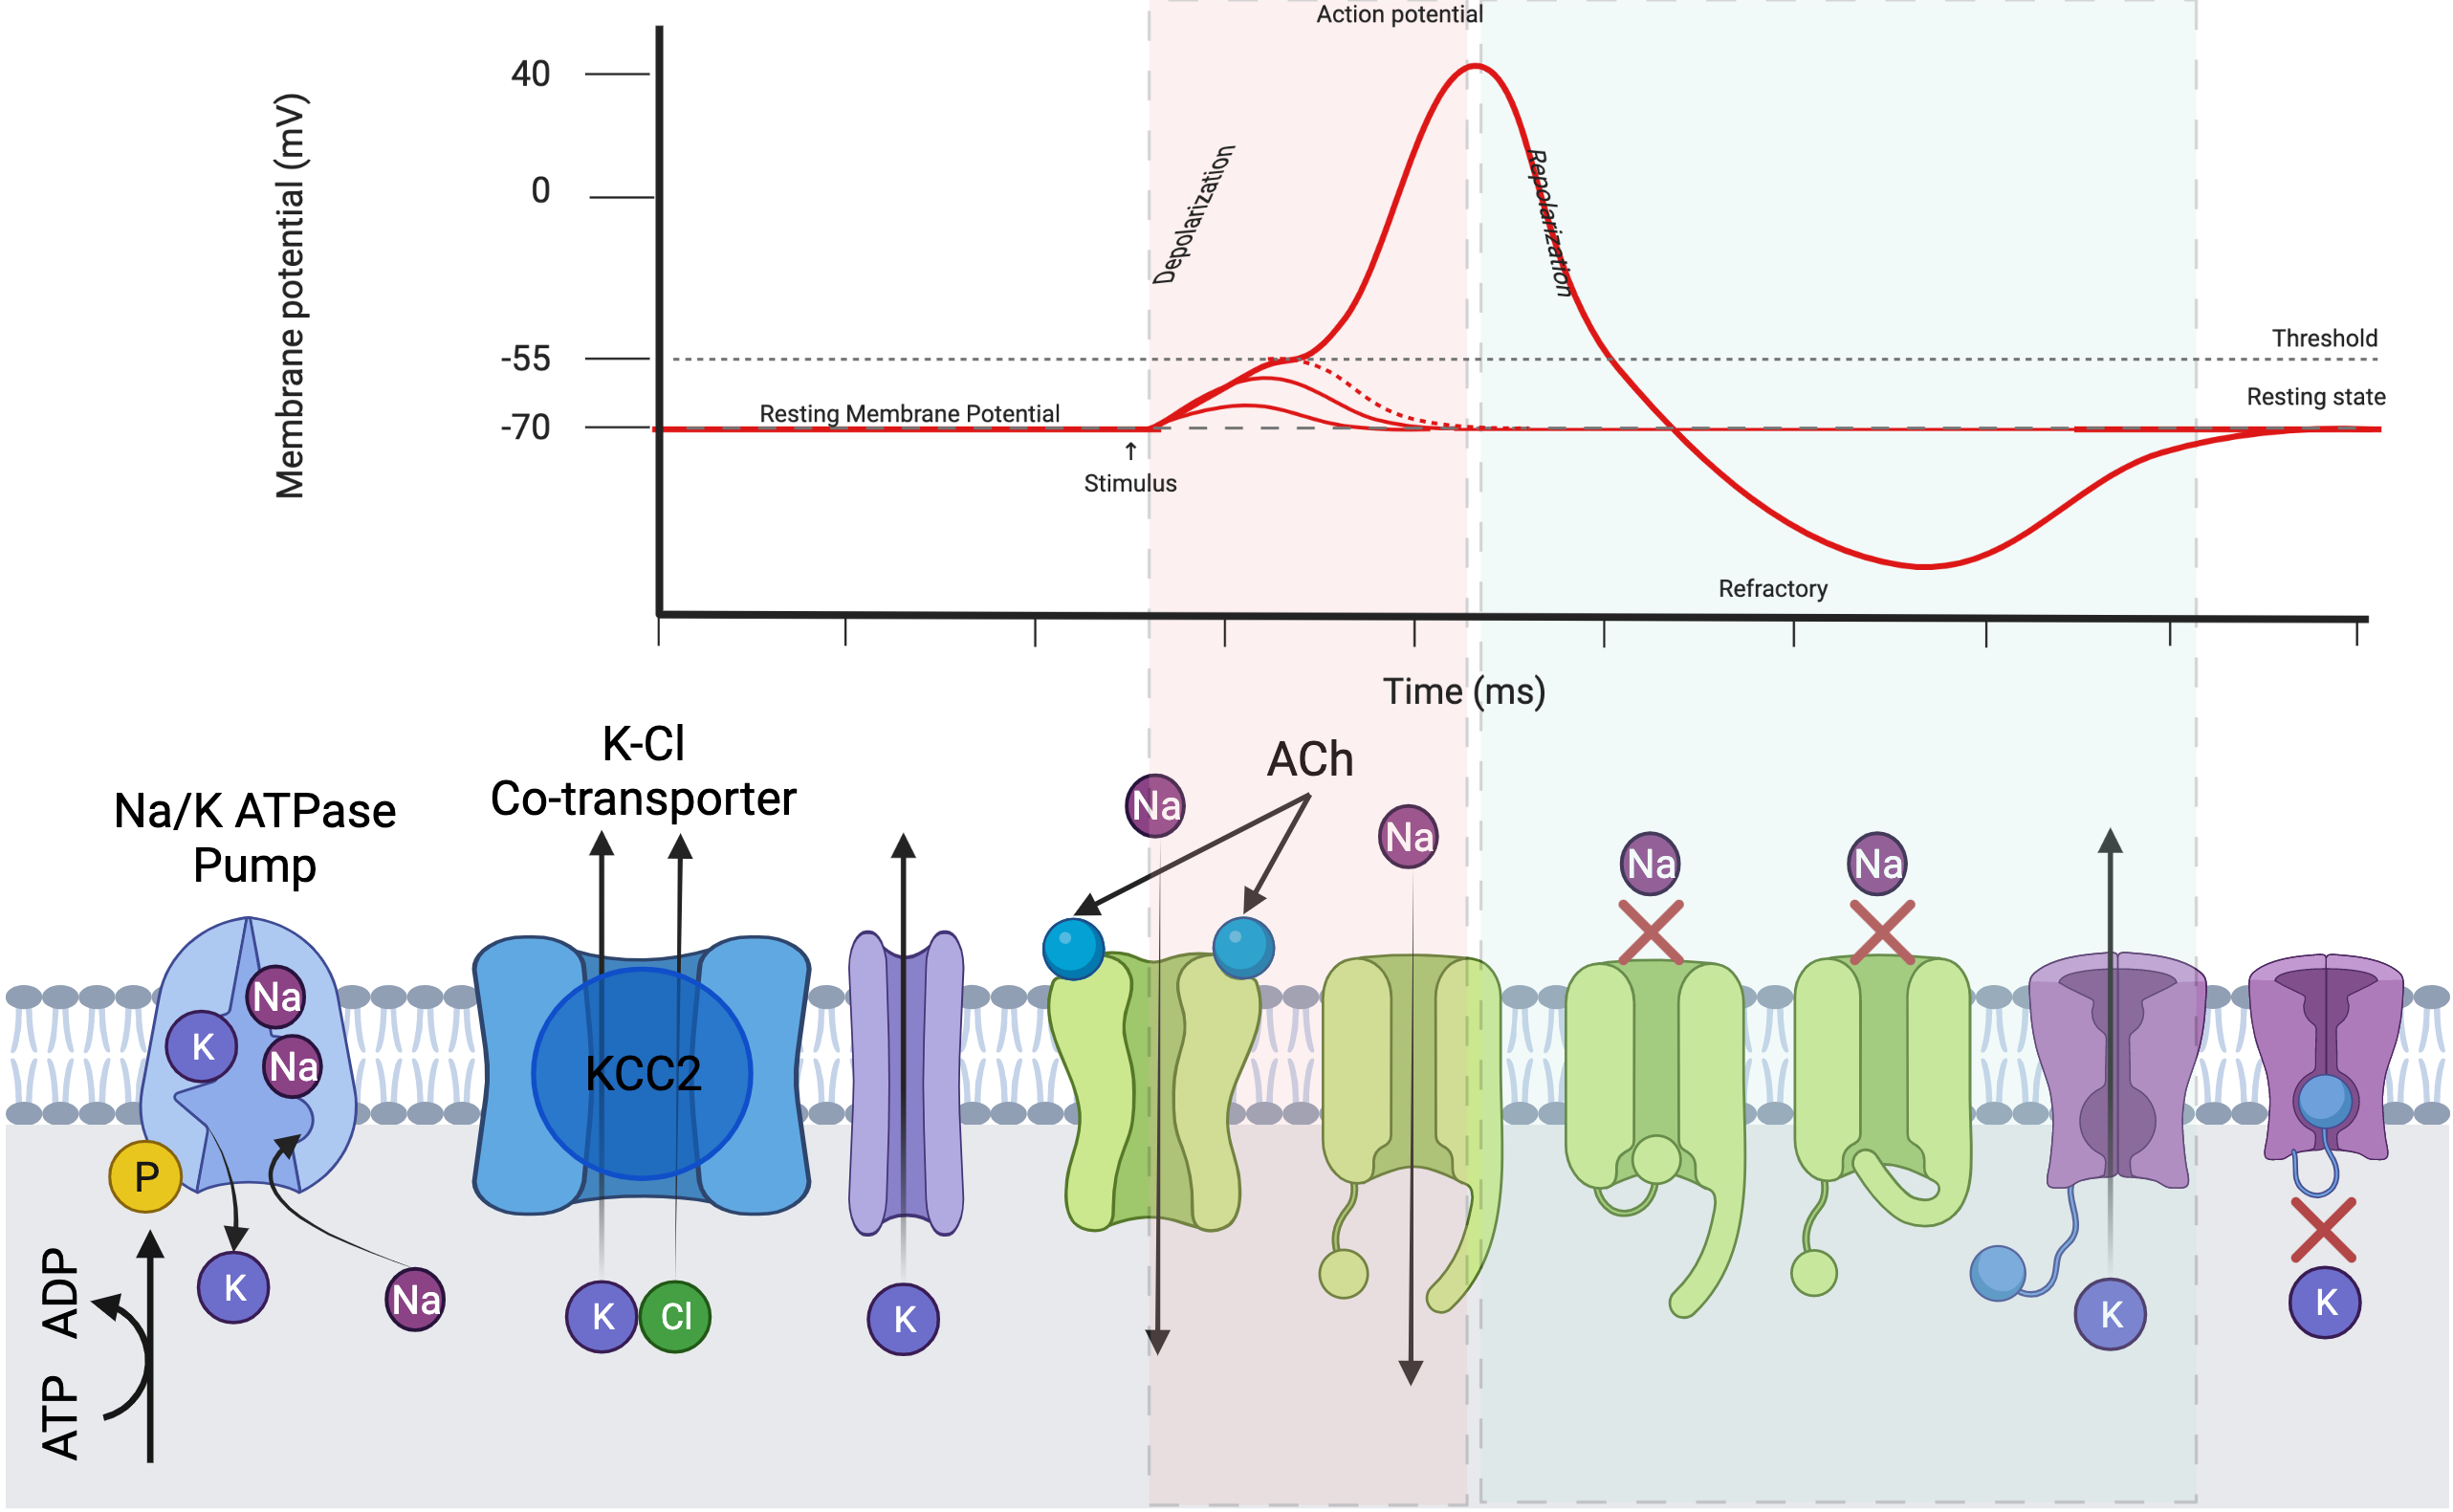
\includegraphics[width=1\linewidth]{./figure/cell_membrane.png}
    \caption{Cell Membrane Components and their general contribution to RMP and an AP \footnotesize{Created with BioRender.com}}
    \label{fig:cell_membrane}
\end{figure}


\paragraph{Pumps \& Transporters}
$Na^+/K^+$ ATPase pumps are embedded throughout excitable membranes. These protein based molecular machines convert the energy of ATP to the movement of three $Na^+$ outside the cell and two $K^+$ inside the cell with each cycle of the pump (each use of ATP). Given the natural tendency of molecules to move based on a concentration gradient (high concentration to low concentration) the resultant higher concentration of  $Na^+$ outside and higher concentration of $K^+$ inside the cell requires the work of these active transport pumps against the concentration gradient.
The $K^+$ - $Cl^-$ co-transporter (KCC2) utilizes the $K^+$ concentration gradient created by the $Na^+$/$K^+$ ATPase pumps to move $Cl^-$ out of the cell as an exchange with $K^+$.


%\begin{figure}
%    \centering
%   \includegraphics{.\figure/pumps.png}
%    \caption{$Na^+/K^+$ ATPase Pumps \footnotesize{Created with BioRender.com}}
%    \label{fig:pumps}
%\end{figure}


\paragraph{Channels \& Receptors}
Channels are proteins embedded in the cell membrane that allow passage of molecules between the intracellular and extra cellular space. Channels can be gated and therefore only allow passage under certain circumstances. 

Voltage gated channels only allow passage when the membrane potential is at certain values. They may open at a certain value and close a certain period of time later; or they may close at a certain value and open a period of time later. 
Ligand gated channels only allow passage when the channel is activated due to the binding of a ligand (a molecule that can bind). A ligand gated channel is also a receptor, or closely associated with a receptor. 

$Na^+$ channels allow the passage of $Na^+$ with its concentration gradient and can be either ligand gated or voltage gated. $K^+$ channels allow the passage of $K^+$ with its concentration gradient and in nerve and muscle excitable membranes are both non gated and voltage gated. Cl channels allow the passage of $Cl^-$ along its concentration gradient and in the sarcolemma are not gated ($Cl^-$ channels are not depicted in \ref{fig:cell_membrane}, but would resemble the $K^+$ channel to the far right of the figure.).

Receptors are proteins that allow ligand binding. Some receptors are ligand gated channels (a receptor where the activity that binding produces is opening a channel gate). Other receptors perform different activities within the cell. 

%\begin{figure}
%    \centering
%    \in$Cl^-$udegraphics{.\figure/receptors.png}
%    \caption{Receptors \footnotesize{Created with BioRender.com}}
%    \label{fig:receptors}
%\end{figure}

\subsection{Establishing the Resting Membrane Potential}

For our purposes the process of establishing the RMP in the sarcolemma focuses on roles played by the concentration gradients and electrical potential created by $Na^+$, $K^+$ and $Cl^-$. Each of these elemental molecules exist in the body as ions (they carry a charge based on whether the have too many electrons ($Cl^-$) or two few electrons ($Na^+$, $K^+$).\footnotemark\footnotetext{Ca is an ion that has 2 more protons than electrons (hence the 2+ superscript in its abbreviation).} 

\subsubsection{Electrical Potentials \& Equilibrium Potential}

% Consider adding Nernst, and Goldman's equations

Movement of molecules across the cell membrane is influenced by the concentration gradient of the ion across the membrane, the permeability of the membrane for that ion and the and the electrical equilibrium potential across the membrane. When we describe electrical potentials the convention is to speak from inside the cell (intra cellular). A negative potential means at the membrane inside the cell there is a negative charge. A positive potential means that at the membrane inside the cell there is a positive charge. We can, for the sake of understanding, simply invert this and say a negative potential means that at the membrane OUTSIDE the cell has a positive charge; and that a positive potential means that at the membrane OUTSIDE the cell has a negative charge.

When an ion moves across a membrane it carries a charge and creates an electrical potential. An important point is that the electrical potential created at the membrane is not created by the concentration gradient, but from the movement of ions which is based on the concentration gradients.  The $Na^+$/$K^+$ ATPase pumps work at a rate in response to the concentration gradients (speed up if there is a need to, slow down to resting levels when able). But even for long periods of high frequency excitations there is no risk of significant change to the ionic concentrations outside or inside the cell. Thinking that there an absolute change in ionic concentration is required for an action potential is a common misconception about action potentials\cite{silverthorn_uncovering_2002}. When $K^+$ moves across the membrane (out of the cell) it creates a negative potential. When $Na^+$ moves across the membrane (into the cell) it creates a positive potential. When $Cl^-$ moves across the membrane (into the cell) it creates a negative potential. 

To generalize these facts. When a positive ion moves into the cell it creates a positive potential; when it moves out of the cell it creates a negative potential. When a negative ion moves into a cell it creates a negative potential; when it moves out of a cell it creates a positive potential. These potentials are based on the movement of the ions, not on their concentration. 

The electrical potential created at the membrane by the movement of an ion then has an influence on the movement of ions. The negative electrical potential created at the membrane by the movement of $K^+$ out of the cell will eventually resist the continued movement of $K^+$ out of the cell. How negative that negative potential needs to be to stop the movement of $K^+$ out of the cell is dependent on the concentration gradient.\footnotemark\footnotetext{It is also dependent on the temperature (which is kept within tight boundaries in the body), Faraday's constant, and the universal gas constant. From these variables the potential generated by any ion can be determined with the Nernst Equation, which is not be covered here at this time.} The electrical potential that stops the movement of an ion is called the \textbf{equilibrium potential}. Figure \ref{fig:equilibrium_potential} shows the concentration gradient and resultant equilibrium potential for our primary ions of interest ($Na^+$, $K^+$, $Cl^-$). Each equilibrium potential in \ref{fig:equilibrium_potential} is based on the assumption that it is the only ion moving across the membrane. In reality they are all moving across the membrane with varying rates which are based on the permeability of the membrane to each ion at any moment in time.\footnotemark\footnotetext{The Goldman-Hodgkin-Katz (GHK) Equation (model) allows the estimation of the membrane potential based on $Na^+$, $K^+$, $Cl^-$ concentration gradients and membrane permeability (along with several other relevant variables. A calculator for the GHK Equation can be found at \url{https://www.physiologyweb.com/calculators/ghk_equation_calculator.html}.}

\begin{figure}[!ht]
    \centering
    %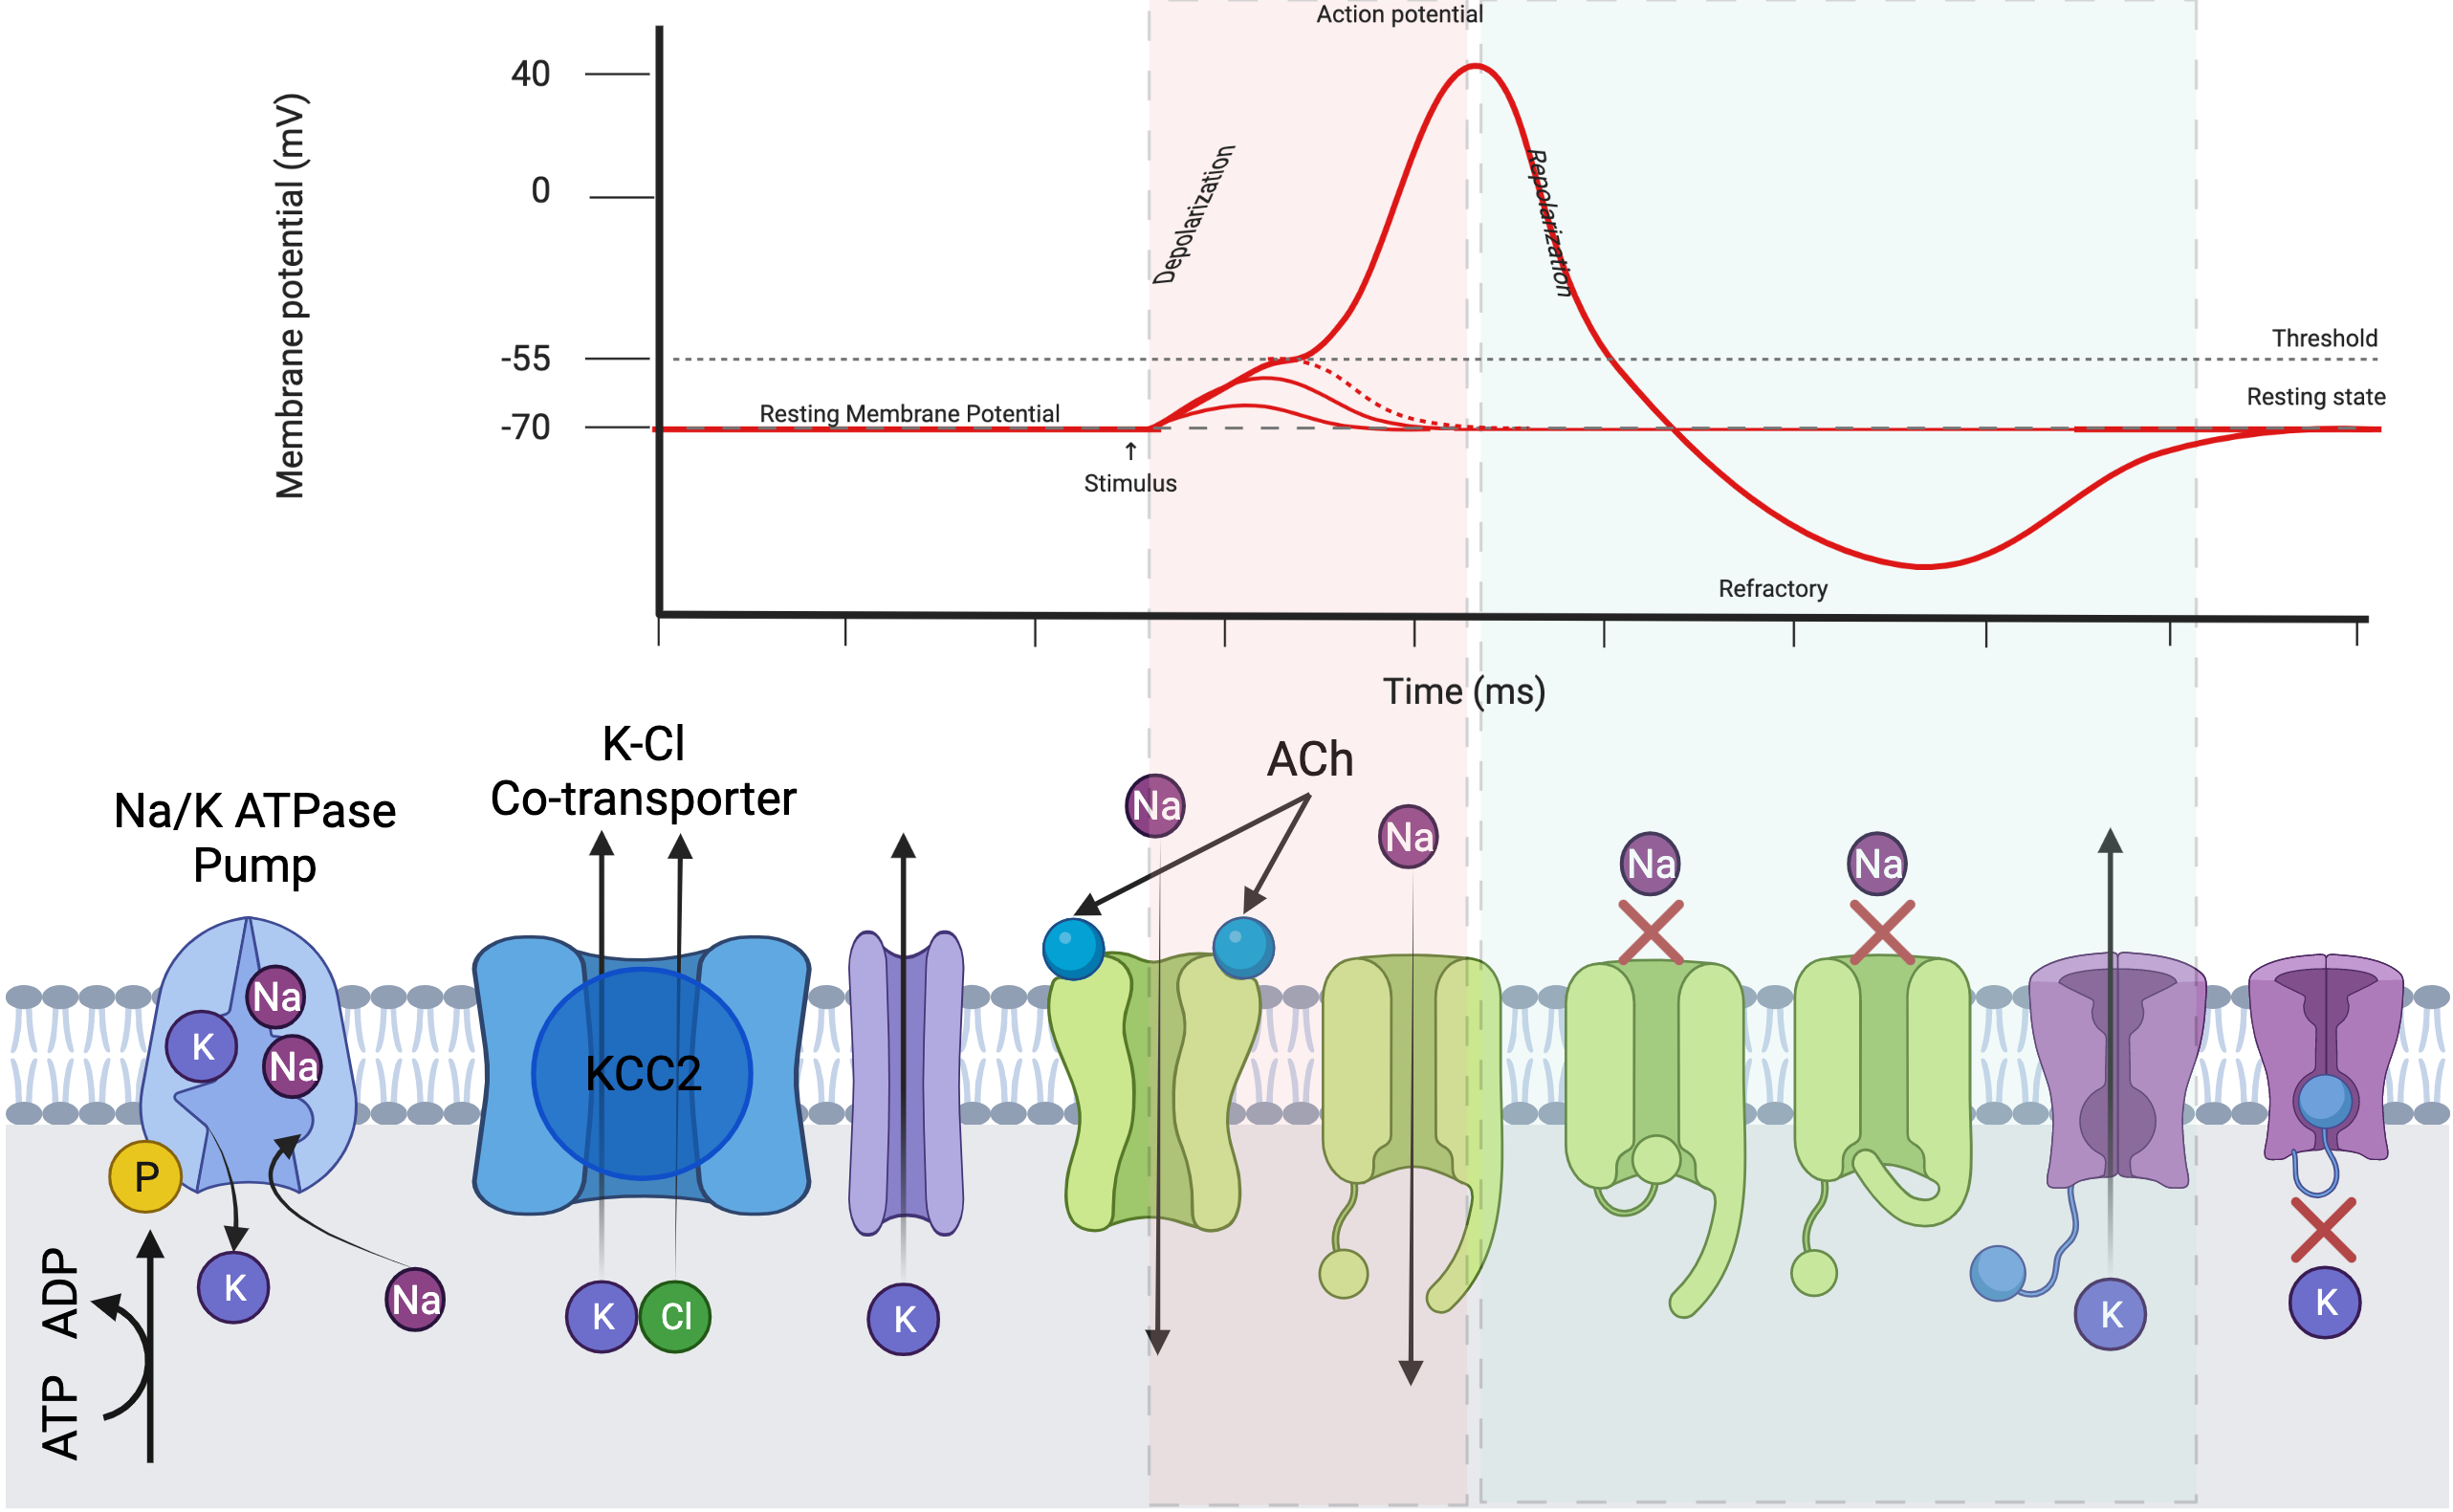
\includegraphics[width=1\linewidth]{./figure/cell_membrane.png}
    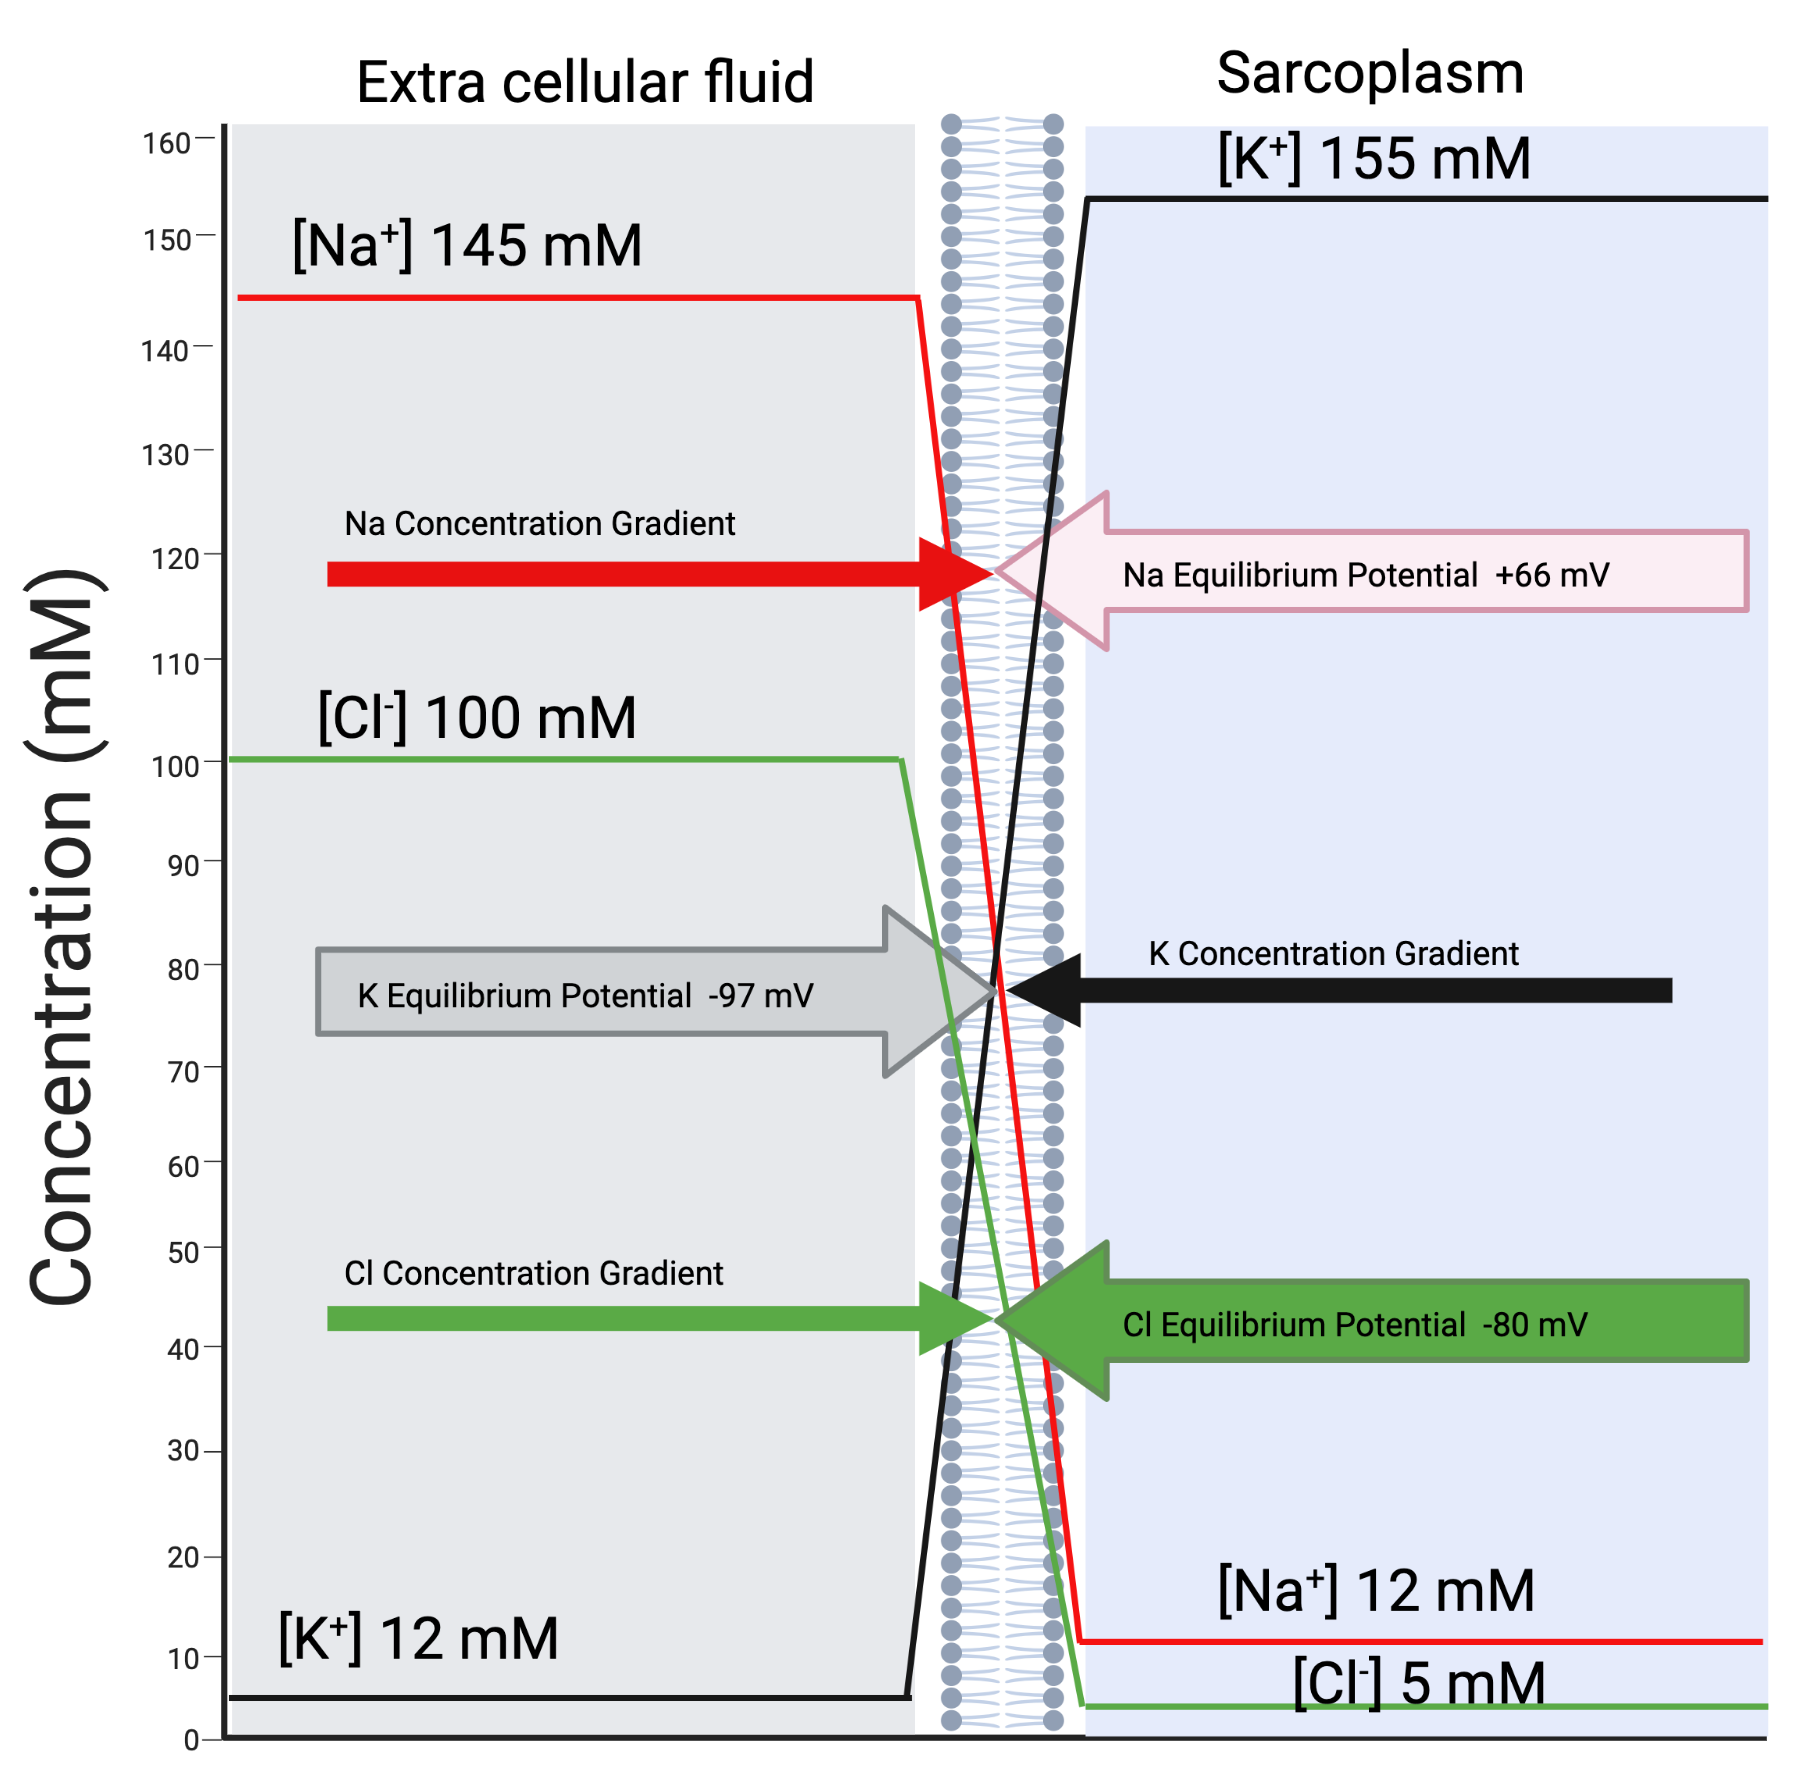
\includegraphics{./figure/equilibrium_potential.png}
    \caption{Generation of Equilibrium Potentials \footnotesize{Created with BioRender.com}}
    \label{fig:equilibrium_potential}
\end{figure}

\paragraph{}
The resting membrane potential is an equilibrium potential. It is the consequence of two physiological situations. First, the presence of large concentration gradients for $K^+$, $Na^+$  and $Cl^-$ across the membrane. Second, the relative permeability of the membrane to these ions. For example, based on Figure \ref{fig:equilibrium_potential}, if $K^+$ was the only ion that the membrane was permeable to at rest the RMP would be equal to the $K^+$ equilibrium potential (about -97 mV).

The concentration gradients for $K^+$ and $Na^+$ are established primarily by the $Na^+$-$K^+$-ATPase pumps. The concentration gradient maintains a large outwardly directed $K^+$ gradient, and a large inwardly directed $Na^+$ gradient. The concentration gradient for $Cl^-$ is maintained primarily through the actions of a $K^+$ - $Cl^-$ co-transporter known as KCC2. Relative to the other ions, there is a moderate inwardly directed $Cl^-$ gradient.

%Change the figure to reduce the size of the gradient vector for Cl-

Since these ions do not pass through the lipid bi-layer of the cell membrane the permeability of the membrane to each ion is tuned by the presence of ion specific channels. Therefore, the relative permeability of the plasma membrane to $Na^+$, $K^+$ and $Cl^-$ is dependent on the number and state (open or closed) of ion-selective membrane channels. Different membranes display different degrees of permeability to different ions, and due to gating mechanisms on many of the ion-selective channels the permeability can be changed (this is a hugely important point considering the entire purpose of an RMP (polarization) is to have the opportunity to generate an AP (depolarization)).

In resting conditions the membrane of nerve and muscle cells are most permeable to $K^+$. In addition to KCC2 allowing movement of $K^+$ out of the cell, there are also non-gated $K^+$ specific ion channels. When combined with the relatively high permeability of $K^+$, the concentration gradient results in a $K^+$ flow out of the cell. As $K^+$ flows out it creates a negative electrical potential. However, the negative electrical potential resists further flow of $K^+$ outside of the cell (and eventually reaches an equilibrium potential). Since $K^+$ has the highest permeability at rest, the resting membrane potential is primarily influenced by the equilibrium potential of $K^+$. It is important to note that while there is no net flow of $K^+$ at the $K^+$ equilibrium potential, $K^+$ is still flowing out of the cell and continues to generate the negative membrane (equilibrium) potential, and $K^+$ continues to be pumped into the cell by the $Na^+$/$K^+$ ATPase pumps. The term "equilibrium" for equilibrium potential means equilibrium in flows (no net flow, no net gain in or outside the cell).

Note from Figure \ref{fig:equilibrium_potential} that the equilibrium potential of $Cl^-$ is close to $K^+$. The implication is that $Cl^-$, despite its concentration gradient encouraging inward flow, does not at RMP, have net inward flow. $Cl^-$ has a higher permeability than $Na^+$ at rest, but a much lower permeability than $K^+$. An important attribute about $Cl^-$ for the sarcolemma and axon membranes is that the permeability of the membrane does not change much, even during an AP. This contributes to the stability of the RMP and helps prevent recurrent self excitation in these membranes.

The equilibrium potential of $Na^+$ is positive (opposite of $K^+$ and $Cl^-$). At RMP the permeability for $Na^+$ is very low, and therefore $Na^+$ has very little impact on the RMP. The importance of $Na^+$ starts when gated $Na^+$ channels start to open - that's when the action begins.

% Old text - don't delete yet
% Under normal, healthy, conditions different cell membranes have slightly different resting membrane (equilibrium) potentials. These differences are due to differences in the permeability of the membranes to $K^+$ (or to other ions, such as $Na^+$, $Cl^-$, $Ca^{2+}$). The extra cellular concentration of these ions is held constant throughout the body and therefore under normal circumstances differences in the concentration gradients are not a major source of differences in resting membrane potentials. 

\subsection{Trigger \& Spread of Sarcolemma Excitation (AP)}

As can be noted in Figure \ref{fig:equilibrium_potential} the equilibrium potential for $Na^+$ is positive. When the membrane relative permeability for $Na^+$ increases (becomes greater than $K^+$ and $Cl^-$) the membrane potential starts to depolarize and even to switch to a positive polarity. This is an action potential. At the molecular level, an action potential is the sudden increase in relatively permeability of the membrane to $Na^+$.  

\paragraph{Triggering the Action Potential (Initial Excitation)}
The events leading to an action potential on the sarcolemma are initiated by the opening of ligand gated $Na^+$ channels by the binding of ACh to these receptors at the motor end plate. The micro potentials created by the opening of the ligand gated $Na^+$ channels by the binding of ACh then open voltage gated $Na^+$ channels due to a change in voltage in the membrane potential (becoming less negative). The number of voltage gated $Na^+$ channels that open is proportional to the change in the membrane potential. This cycle of opening in response to a voltage change is self perpetuating since once a $Na^+$ channel opens $Na^+$ flows into the cell due to the $Na^+$ concentration gradient. Due to the movement (not a change in the actual gradient) the membrane potential voltage changes (becomes less negative) as the potential moves toward the $Na^+$ equilibrium potential. The point that approximately half of the voltage gated $Na^+$ channels open is considered a threshold potential. At the threshold potential the voltage gated $Na^+$ channels continue to rapidly open until the equilibrium potential approaches that of $Na^+$ (as opposed to $K^+$) since at this point the membrane is more permeable to $Na^+$. The equilibrium potential for $Na^+$ is approximately 66 mV.  Once a membrane reaches the threshold potential an action potential is inevitable. It is at this point that the action potential is said to be “all or none.” Prior to the threshold potential membranes can undergo micro potential changes. These micro potentials can be depolarizing (excitatory potentials that move the membrane potential toward the threshold), or hyperpolarizing (inhibitory potentials that move the membrane potential further away from the threshold potential). The use of micro potentials to regulate muscle tension is an important part of Chapter \ref{chp:regulation} since it is a process that occurs at the $\alpha$-motor neuron dendrites in the spinal cord, not at the NMJ.\footnotemark\footnotetext{An $\alpha$-motor neuron, once excited, will release only one neurotransmitter, ACh at its axon terminal. ACh will only have one effect at the NMJ, creating excitatory micro-potentials on the motor end plate. However, in the Central Nervous System (such as the Spinal Cord) competing neurotransmitters can be released at synapses of the $\alpha$-motor neuron dendrites. The impact of these neurotransmitters can be excitatory or inhibitory. Since they occur after the synaspse they are called excitatory post synaptic potentiations (EPSPs) or inhibitory post synaptic potentiations (IPSPs). Whether, and how frequently, an $\alpha$-motor neuron sends an excitation to the muscle fibers it innervates is balanced by competition between the EPSPs and the IPSPs.}

\paragraph{Spread of the Action Potential (Wave of Excitation)}

The wave of excitation of the AP across the sarcolemma and T-tubules occurs due to the self-perpetuating opening of voltage gated $Na^+$ channels. When a region of the membrane depolarizes it opens the nearby voltage gated $Na^+$ channels which depolarize that region, which then opens the nearby voltage gated $Na^+$ channels which depolarize that region, "And so it goes."\footnotemark\footnotetext{A quote for other Kurt Vonnegut fans.)}

Of course, there cannot be an AP if there is no RMP. Therefore, the AP must end. The membrane must repolarize to be ready for another depolarization. Considering muscle tension is, partly, regulated by how frequently it experiences excitation (which can reach upwards of 180 Hz, that is 180 excitations per second, for those excitations to occur there need to be an equal number of repolarizations).

The process of repolarization occurs in two steps. Voltage gated $Na^+$ channels have two gates. One is an activation gate and it is closed under resting conditions and opens during excitation. The second is an inactivation gate and it is open under resting conditions but closes soon after the activation opens. The inactivation gate closure is timed, it is not triggered by events outside of the molecule itself. Closing the inactivation gate is the first step to stopping an action potential. The closure of the inactivation gates reduces the relative permeability of $Na^+$. While the activation gate is open and the inactivation gate is closed the membrane is in the absolute refractory period (cannot undergo depolarization regardless of how great an excitation stimulus may be). To be reset and completely ready for another action potential the activation gate must close and the inactivation gate must open (these are timed events).

The second step (really second part, do not think of these in an overly temporal manner since events overlap in time) to repolarization is opening of voltage gated $K^+$ channels. These are delayed (take longer to open than the voltage gated $Na^+$ channels). Once the voltage gated $K^+$ channels open the membrane permeability to $K^+$ increases higher than under resting conditions which further expedites the repolarization process and can also result in a hyper polarized state (slightly more negative membrane potential than the normal resting membrane potential). Closing the voltage gated $K^+$ channels is also a timed event. While they are open the membrane is in a relative refractory period. It is resistant to excitation, however, with an increased stimulus it can be excited.

The overall process of repolarization and return to the resting membrane potential takes approximately 3-4 milliseconds (ms). Assuming 3 ms is the fastest interval for another AP, the upper limit on excitations would be approximately 333 Hz (which exceeds the maximum capacity for muscle fiber twitches per second).

Spread of excitation occurs in one direction (meaning it does not result in cyclic repeating action potentials of the entire membrane) because of the refractory periods. If a membrane is visualized as a set of dominoes and the resting potential is when the dominoes are upright, and an action potential is when a domino falls, then the refractory period is the period when the domino is still fallen. Because of the fallen domino on one side of the next falling domino, the dominoes fall in one direction away from the starting stimulus. A further safeguard against cyclic repeating actions potentials in the sarcolemma is the constant permeability for $Cl^-$ in the sarcolemma. Recall that at RMP $Cl^-$ has no net flow because its equilibrium potential is near the $K^+$ potential. When the membrane potential fluctuates away from the the $K^+$ (and $Cl^-$) equilibrium potential there is net movement of $Cl^-$. This $Cl^-$ net movement (into the cell) contributes to repolarization but also to stability of the RMP in the moments following an AP. In situations such as myotonia congenita altered membrane $Cl^-$ permeability leads to a higher occurrence of myotonia (sustained muscle tetany) due to recurrent muscle excitation from cyclic repeating action potentials \cite{adrian_action_1976}.

\subsection{Excitation to Regulation}

This section has taken a deeper dive into the molecular events of excitation than the previous section. It should be clear that many events must occur for one excitation, particularly since one excitation creates a twitch, and a twitch is not enough to produce meaningful movement. A more efficient system of excitation-activation coupling exists in the cardiac muscle. However, in the skeletal muscle the efficiency of creating tetany from one excitation is sacrificed for the sake of regulation of muscle tension. Since creating tetany requires many action potentials, then the amount of tetany, and therefore the amount of tension, can be regulated by the number of action potentials. The regulation of muscle fibers is the topic for Chapter \ref{chp:regulation}.


\section{\textit{Clinical Physiology Connections}}

The concepts of excitable membranes, receptors, ligand channels and signal transduction are pervasive throughout clinical physiology. This final section of the chapter introduces some clinical physiology connections that are now possible given your understanding of excitable membranes, including the neuroendocrine system, sensory receptors and pharmacodynamics. These topics return throughout the book in particular contexts.

\subsection{Neuroendocrine}

The neuroendocrine system regulates several critical physiological systems and coordinates cellular functions throughout the body. Examples include mobilizing the body for fight or flight reactions by getting all cells in the body ready to meet demands that require energy mobilization at the expense of other maintenance activities. For example, release of hormones for fight or flight signals liver cells to hold off on using energy to maintain the cell membrane and instead use energy to convert glycogen (a stored fuel) into glucose (a usable fuel). The neuroendocrine system can alert cells all over the body to do activities that each of those cells can do for the fight or flight situation, even though those activities are varied between the cells. While the liver cells are releasing glucose, the heart cells are prepared to use more glucose and are working more frequently (higher rate) and harder (more pressure). The differentiation and variety of tasks completed by these cells is due to the specialization of the cells, and due to the receptors around the body that are responding to the same ligand. Most cells in the body have a ligand receptor for epinephrine (a major catecholamine of the fight or flight response). Epinephrine is also called adrenaline. Receptors for epinephrine are therefore called adrenergic receptors. The adrenergic receptors on all cells have a similar binding location for epinephrine, but the receptor itself transducts different signals into the cell depending on the receptor and depending on the cell. For example, the adrenergic receptors on smooth muscle in arterioles in the systemic circulation signal contraction which results in vaso-constriction. However, the adrenergic receptors on smooth muscle in bronchioles in the lung signal relaxation, which results in broncho-constriction.

The fight or flight (alert) response from the neuroendocrine is a coordinated response of the component of the central nervous system called the autonomic nervous system, and in particular the sympathetic nervous system (SNS). The SNS is a truly neuroendocrine system because it has both nervous system and endocrine components. Ligands for the SNS, epinephrine and norepinephrine, are also both neurotransmitters and hormones.

For homeostasis (balance), if there is a fight or flight (alert) system then there should also be a rest, digest and reproduce (chill) system. The chill system is the parasympathetic system (PNS). The PNS is a nervous (but not neuroendocrine) system. The connections through the body of the PNS are all mediated with nerve function and neurotransmitters (not endocrine, or hormone signals). This is not to say that the during a chill situation hormones are not involved. Just that if there are pathways through which the PNS mediates those chill (rest, digest, reproduction) hormones they have not been discovered yet (at least as far as the author knows as of \today). The primary neurotransmitter for the PSN is acetylcholine (ACh). The PNS receptors that bind ACh are called cholinergic receptors. 

\subsection{Sensory Receptors}

Sensory receptors are specialized receptors at the terminal end of the axon of a sensory neuron. They differ from ligand and voltage gated receptors in the signals that provokes their excitation. When a sensory receptor is excited it sends an afferent signal (to the central nervous system, as opposed to efferent signal, away from (or exiting) the central nervous system). In general, the signal the provokes excitation in a sensory neuron is whatever phenomenon or sensation that sensory neuron is associated. If the sensory neuron is excited by changes in temperature then it is a temperature sensory neuron; if by changes in tension, it is a tension sensory receptor; if by vibrations, it is a vibration (as in the ear) sensory receptor; if by photons, it is a light sensory receptor (as in the retina); if by certain chemicals or ions (such as $H^+$ for pH, or carbon dioxide, or oxygen) they are chemoreceptors; if by changes in pressure they are baroreceptors. Some sensory receptors terminate in areas of the brain that allow perceptions of the signal in a way that gives them additional meaning. For example, some chemoreceptors proceed to the brain and produce pain signals, once in the brain a complicated cascade of connections are made that can, over time, change from being protective to themselves harmful to movement. Other chemoreceptors that detect an increase in carbon dioxide proceed to areas in the nervous system to produce unconscious reflex responses (changing respiratory rate) and also to the brain (a general state of anxiety and air hunger). Some receptors don’t go to the brain at all, but interact at areas in the nervous system where responses are automatic (baroreceptors as part of the autonomic nervous system to regulate blood pressure). Since baroreceptors don’t go beyond the brain stem we do not perceive what our blood pressure is directly - making elevated blood pressure a “silent killer.” To be a homeostatic regulatory system there needs to be a sensory receptor of some type that contributes to the monitoring of the homeostatic variable. So a homeostatic regulatory system includes a homeostatic variable that is sensed by a sensory receptor that sends an afferent signal to be processed (often not perceived), which then sends an efferent signal to exert an action which aims to adjust the homeostatic variable. The neuroendocrine system is commonly involved in such systems, receiving afferent signals, and sending efferent signals. Most physiological homeostatic systems are negative feedback systems, which means sensation of an increase in a variable triggers response to decreases that same variable (and vice versa).

\subsubsection{Sensory Receptor Dynamics}
Sensory receptors are proteins embedded in cell membranes. Therefore, the cell has control over some dynamic and important behavior of these receptors (indeed, all receptors).  Up-regulation is a term for sensory receptor dynamics that includes an increase in the number of receptors. Down-regulation is a term for sensory receptor dynamics that includes a decrease in the number of receptors. With up-regulation or down regulation there are changes to the strength of a excitation and therefore signal sent to the respective neurons. For example, with up-regulation of chemoreceptors for carbon dioxide an individual will have a higher respiratory rate and maintain a lower carbon dioxide level since their response to carbon dioxide is increased. The up-regulation then continues to propagate itself. Since it results in lower carbon dioxide levels, the receptors remain up-regulated in an attempt to be able to respond to the lower carbon dioxide levels. A balance point is eventually achieved. But this new balance point may be enough to result in what is converted altered homeostasis. In individuals taking a beta-blocker (beta-adrenergic blocker medication) the lack of cardiac response to neuroendocrine stimulus results in higher adrenaline levels. The adrenergic receptors of the heart down-regulate in response to higher circulating adrenaline which further blunts cardiac responsiveness to adrenergic stimulation. A balance point is eventually achieved as with the previous example, however, the individual has an alteration to homeostasis. 

\subsubsection{Neuromuscular Sensory Receptors} 
There are several important neuromuscular sensory receptors that sense signals from the muscle, musculotendonous junction and/or the tendon. Signals for tension (such as golgi tendon organs), signals for changes in length (such as the muscle spindle), and signals for the chemical constituents of the extra cellular fluid surrounding muscle fibers (chemoreceptors). These receptors and their role in muscle function is covered in upcoming chapters on regulation, energetics and micro-circulation.

\subsection{Pharmacodynamics}

Pharmacology is divided into pharmacotherapeutics and toxicology. Toxicology focuses on the harmful effects that chemicals, such as medications, may have on the body. Pharmacotherapeutics is the development and study of medications. Pharmacotherapeutics is divided into pharmacokinetics and pharmacodynamics. Pharmacokinetics focuses on the absorption, distribution and metabolism of medications. Pharmacodynamics focuses on the intended systemic and cellular effects of medications. Pharmacodynamics is therefore a study of the actions of medications in the body. The cellular and systematic effects of a medication is often related to what receptors it binds, what neurotransmitter or hormone it effects of mimics, or what signal transduction mechanism it influences. Pharmacodynamics often includes changes to the process of excitation discussed in this chapter.

\subsubsection{Curare}
Curare is paralyzing agent. It stops the excitation of the motor end plate. It does so by competitively and reversibly binding to ACh receptors on the motor end plate which blocks those receptors from binding with ACh. When curare binds to an ACh receptor it does not open the ligand gated $Na^+$ channel and therefore prevents the initiation of depolarization. As a competitive binding, curare blocks the ACh receptor and thus inhibits the ACh binding and response. Another term for competitive binding is that curare is an antagonist (blocks without producing an effect). Some medications are agonists, they bind and create an effect and are thus utilized to facilitate additional cellular activity beyond that of the normal ligand. As a reversible binding medication, curare can be removed from the ACh receptor. Medications can also create irreversible binding. Curare is also selective, it only binds to skeletal muscle motor end plate ACh receptors. Which means it selectively inhibits these receptors and not other ACh receptors throughout the body. This means the systemic response is limited to skeletal muscle paralysis. If used during surgery without other anaesthetics it would produce paralysis but no change in pain sensation, a very unpleasant surgery that would be stopped when the pain and anxiety of the procedure produced a rapid heart rate and rising blood pressure due to the fight or flight response of the neuroendocrine system (which would not be stopped by curare). In addition to surgical or intensive care situations, curare can be used as a poison, causing death by asphyxiation since the muscles of ventilation (breathing) are skeletal muscles. 

\subsubsection{Medication Induced Receptor Dynamics}
A consequence of medications is that they can produce changes in receptors. Up-regulation and down-regulation of receptors due to their pharmacodynamics are a common reason for the need to carefully, and only under supervision, withdraw a dose of medications. If the medication led to up or down regulation and depending on whether it is a receptor antagonist or agonist, could have big implications with sudden cessation. For example, if a medication leads to down regulation of receptors, cessation of that medication could result in a large drop in cellular activity (whatever that activity may be). For example, serotonin re-uptake inhibitors are antagonists that block the re-uptake of serotonin in synapses of the central nervous system. This increases the amount of serotonin which can lead to down-regulation of the serotonin receptors. If the medication is suddenly stopped there will be less serotonin and less receptors (due to down-regulation) which magnifies the effect of having less serotonin, potentially worsening of the original reasons for taking the medication. 

\subsubsection{Autonomic Nervous System Medications}

There are several medications that influence the autonomic nervous system function for a variety of health conditions. Applying what we know about receptors and pharmacodynamics it should be clear that an adrenergic agonist will increase SNS activity in the cell that the medication binds to, whereas an adrenergic antagonist (blocker) will reduce the SNS activity in the cell that the medication binds. A cholinergic agonist will increase the PNS activity in the cell, whereas a cholinergic antagonist will decrease the PNS activity in the cell. Very simple. Two types of receptors that can effect the receptors in two ways and therefore can create four different cellular responses. 

Thankfully there is enough cholinergic receptor specificity that a cholinergic agonist with the therapuetic goal of changing gut motility is specific to the cholinergic receptors in the gut. If all cholinergic receptors were the same, then such a cholinergic agonist could cause wide spread muscle spasms.

\section{Summary \& Next Steps}

Muscle fiber excitation starts with an excited motor axon ($\alpha$-motor neuron) and ends with the binding of calcium to troponin, which generates a twitch (the fundamental unit of active tension). Binding calcium to troponin allows a crossbridge to go from an inactivated to an activated state. The final step in muscle excitation is the coupling between excitation and activation (Excitation - Activation Coupling). The underlying molecular mechanisms involve the characteristics and actions of excitable membranes. Excitable membranes require ion channels, pumps and receptors. Actions include using transport to establish a resting membrane potential and the ability to have an action potential (excitation). Understanding excitable membranes creates Clinical Physiology Connections opportunities in three areas: 1. system wide regulatory function of the neuroendocrine system; 2. function of sensory receptors; and 3. pharmacodynamics.

A twitch is the fundamental unit of muscle fiber active tension. A twitch is activated by excitation of the muscle fiber by the $\alpha$-motor neuron. Excitation of the muscle fiber is the fundamental unit of regulating active tension in the muscle fiber. The next chapter considers regulation as the process of varying muscle fiber excitation - both the frequency of excitation as and the number of muscle fibers excited.


\printbibliography[heading=subbibintoc]




% !TEX root = ../notes_template.tex
\chapter{Muscle Regulation}\label{chp:regulation}
Updated on \today
\minitoc

This chapter introduces the mechanisms utilized by the central nervous system (CNS) to regulate active tension. To regulate active tension means to vary its force from its lowest value (resting tone) to its maximal value (maximal voluntary contraction (MVC)). Active tension is developed at the level of the sarcomere, excitation at the level of the muscle fiber, regulation occurs at the level of motor units. A motor unit includes an $\alpha$-motor neuron and all of the muscle fibers it innervates. The CNS has two strategies to regulate active tension. One strategy is to manipulate the number of twitches per second (frequency summation or rate coding); and the second strategy is to manipulate the number of motor units twitching (motor unit summation or motor unit recruitment). Between these two approaches there is a nearly continuous variation in active tension possible, with some muscles (fine motor) having a greater capacity for continuous variation than others (gross motor).

\vspace{5mm}

\textbf{Objectives include:}
\begin{enumerate}
    \item Explain motor unit structure–function relationships.
    \item Explain muscle fiber differentiation (types) structure-function relationships.
    \item Explain motor unit excitation, twitch and tetany.
    \item Compare and contrast frequency summation (rate coding) and motor unit summation (recruitment).
    \item Explain the order of recruitment.
    \item Explain how the muscle spindles and the golgi tendon organs influence motor unit excitation.
    \item Explain the physiological basis of the electromyogram (EMG) and limitations of EMG interpretation.
    \item Explain the effect of amyotrophic lateral sclerosis and aging on motor units.
    \item Explain the effect of peripheral nerve demyelination on muscle regulation.
\end{enumerate}\

\section{Motor Units}

A motor unit is an $\alpha$-motor neuron and all of muscle fibers that its terminal axon branches form a neuromuscular junction at a motor end plate. Each muscle fiber has one motor end plate, and therefore one neuromuscular junction. However, each $\alpha$-motor neuron has many terminal axon branches. The muscle fibers of a single motor unit are randomly dispersed throughout the muscle epimysium. Therefore, the muscle fibers of a motor unit contribute to the tension developed in several fascicles. This arrangement ensures that when only a few motor units are excited there are muscle fibers throughout the entire muscle generating tension at the tendon attachments to avoid asymmetrical pull from one fascicle or isolated location within the epimysium.

\begin{figure}[!ht]
    \centering
    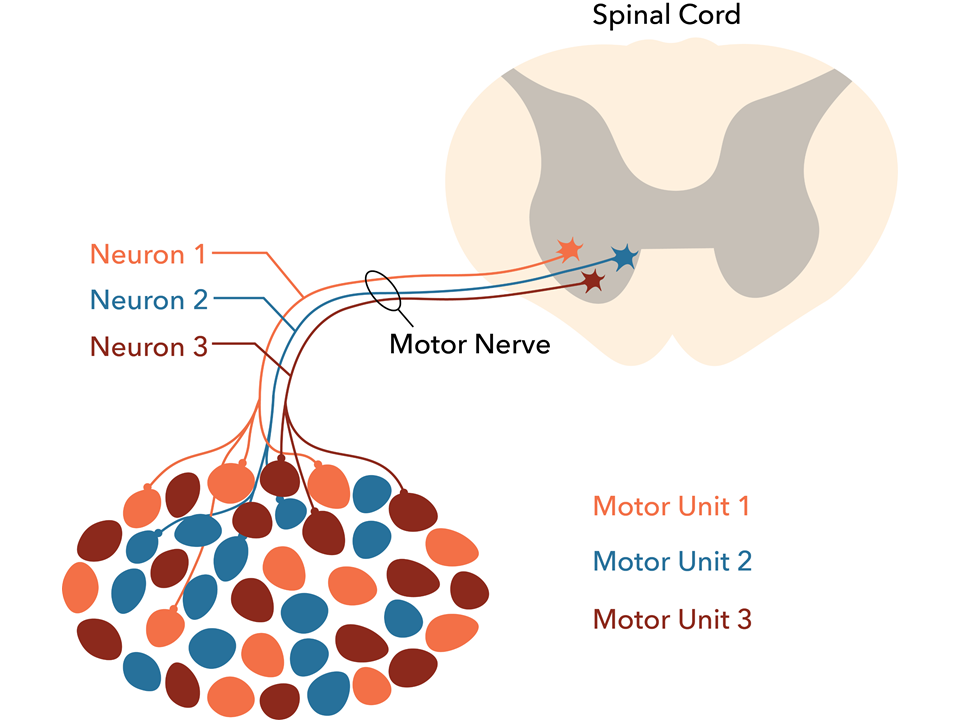
\includegraphics[width=1\linewidth]{./figure/motor_unit.png}
    \caption{Motor Unit Distribution in a Muscle \footnotesize{\href{https://commons.wikimedia.org/wiki/File:Motor_unit.png}{Wikimedia Commons, CC BY 4.0})}}
    \label{fig:motor_unit}
\end{figure}

\subsection{Innervation Ratio}
Motor unit innervation ratio (IR) refers to the number of muscle fibers per motor unit and is usually given as the average number of muscle fibers per motor unit.

\begin{equation}
    IR = \frac{N_{mf}}{N_{mu}}
\end{equation}

The IR varies between muscles and differentiates muscles equipped for fine or gross motor control (See Table \ref{table:Innervation_Ratios}). IRs vary from 5 in muscles in the eye (i.e. lateral rectus) to approximately 1700 in muscles in the calf for locomotion (i.e. gastrocnemius).

\begin{table}[h!]
\centering
\begin{tabular}{||c c c c||} 
 \hline
 Muscle & $\alpha$-motor neurons & Muscle Fibers ($\times 10^3$) & Innervation Ratio \\ [0.5ex] 
 \hline\hline
 Lateral Rectus (eye) & 30* &.15* & 5 \\
 Lumbricals (hand) &  98 & 10.3 & 105 \\ 
 Brachialis & 330 & 130 & 393 \\
 Biceps  & 774 & 580 & 749 \\ 
 Gastrocnemius & 580 & 1000 & 1724 \\[1ex] 
 \hline
\end{tabular}
\caption{Variability of Innervation Ratio in Human Muscles (\footnotesize{From \cite{buchthal_motor_1980}, (* Estimates that need confirmation)})}
\label{table:Innervation_Ratios}
\end{table}

IRs for whole muscles are explanatory for the concept of fine motor and gross motor control. Considering tension is developed by muscle fibers, the number of muscle fibers recruited with each new motor unit recruited influences the size of jumps in active tension. Muscles with lower IRs have greater regulation (control) over the amount of tension they produce because they better accommodate continuous increments in tension with each new motor unit recruited. Of five muscles in Table \ref{table:Innervation_Ratios}, the lateral rectus (eye) and lumbricals (muscle in the hand) have the greatest fine motor control. While the gastrocnemius is responsible for the greatest need for high tension (force) output (gross motor control).

\subsection{Motor Unit \& Muscle Fiber Types}

While IRs for whole muscles help explain variation between muscles with differences in motor control they ignore the systematic variation in the number of muscle fibers per motor unit within a muscle. There are different types of motor units. The types include differences in the $\alpha$-motor neurons, the muscle fibers and the IR. The differences are structural and functional. Types exist on a spectrum with transitions in many (but not all) of the characteristics between them. Despite the spectrum, and using different characteristics, experts have identified and agree on classification systems that converge on three types of human motor units and associated muscle fibers \cite{lieber_skeletal_2010}.

\begin{itemize}
    \item Fast Fatigable (FF) Motor Units with Fast Glycolytic (FG) (Type 2a) Muscle Fibers
    \item Fast Resistant (FR) Motor Units with Fast Oxidative (FOG) (Type 2x) Muscle Fibers
    \item Slow (S) Motor Units with Slow Oxidative (SO) (Type 1) Muscle Fibers
\end{itemize}

The above classification names are all utilized, however the Type 1, 2x and 2a are probably the most common. The other classifications are informative about the functional characteristics of the motor units and muscle fibers they innervate. Beyond their coherence, the motor unit classifications FF, FR and S share a feature with the muscle fiber classifications FG, FOG and SO. They both use the letters F and S to represent Fast and Slow, and they primarily refer to faster or slower excitation (and in the case of muscle fibers also activation). 

The second letter F in FF, and the letters R and S (dual use of the meaning slow for the Slow motor units), and the letters G and O for muscle fibers are related to functional characteristics of fatigue and energetics. For motor unit classifications the second F in FF stands for fatigable, meaning FF fibers are fatigable and cannot sustain tetany for very long. The R in FR motor units stands for resistant, as in fatigue resistant. They resist (for a time) the fatigue of FF motor units. And the S motor units are slow, both in excitation, and slow to fatigue (hence the "dual use" of slow). In Chapter \ref{chp:energetics} on Energetics, the concept of fatigue denoted in muscle fiber classification letters G and O refer to the biochemical pathways that produce ATP, glycolosis and oxidative (including both the citric acid (Kreb's) cycle and electron transport). The connection between FF and FG, FR and FOG, and S with SO, has to do with the rate and sustainability of ATP production by these pathways. Glycolosis has a relatively high rate and low sustainability, and oxidative pathways have a relatively low rate and high sustainability. These pathways, but not just these pathways, result in the fatigability, fatigue resistant or slow to fatigue characterizations of motor units and their fibers. While fatigability comes up in this chapter, the focus is on the excitation and activation characteristics of the fast and slow motor units and muscle fibers.

\subsubsection{Fast vs. Slow - An excitable concept}

The terms fast and slow refer to relative differences in functional characteristics between $\alpha$-motor neuron and the muscle fibers. The functional characteristics fast and slow are associated with a set of functionally coherent structural differences. The section below focuses on the most distinguishing structural characteristics that influence the functional characteristics of excitation and activation.

\paragraph{Fast \& Slow $\alpha$-Motor Neurons}
Fast and slow for the motor unit $\alpha$-motor neuron refers to how quickly excitations can be sent which influences how frequently they can be excited. The faster an excitation propagates down an axon the sooner it is ready for another excitation. In a sequence of excitations, if a second excitation catches up to the first excitation it will cease propagation once it reaches a section of the axon membrane that is its refractory period from the first excitation. A fast neuron has a higher nerve conduction velocity (NCV) and a higher maximum excitation frequency (Hz) than a slow neuron.

NCV is related to the size of the neuron (diameter) because diameter influences resistance to current. Current is the flow (flow is a rate) of electrical impulses and therefore directly related to velocity. Diameter is inversely proportional to resistance, and resistance is inversely proportional to current, therefore diameter is directly proportional to current and velocity (See Figure \ref{fig:Current_Resistance}). The large diameter of the $\alpha$-motor neurons, combined with the myelin sheaths (The role of myelin was introduced in Chapter \ref{chp:excitation}), contribute to its relatively high NCV. 

\begin{figure}[!ht]
    \centering
    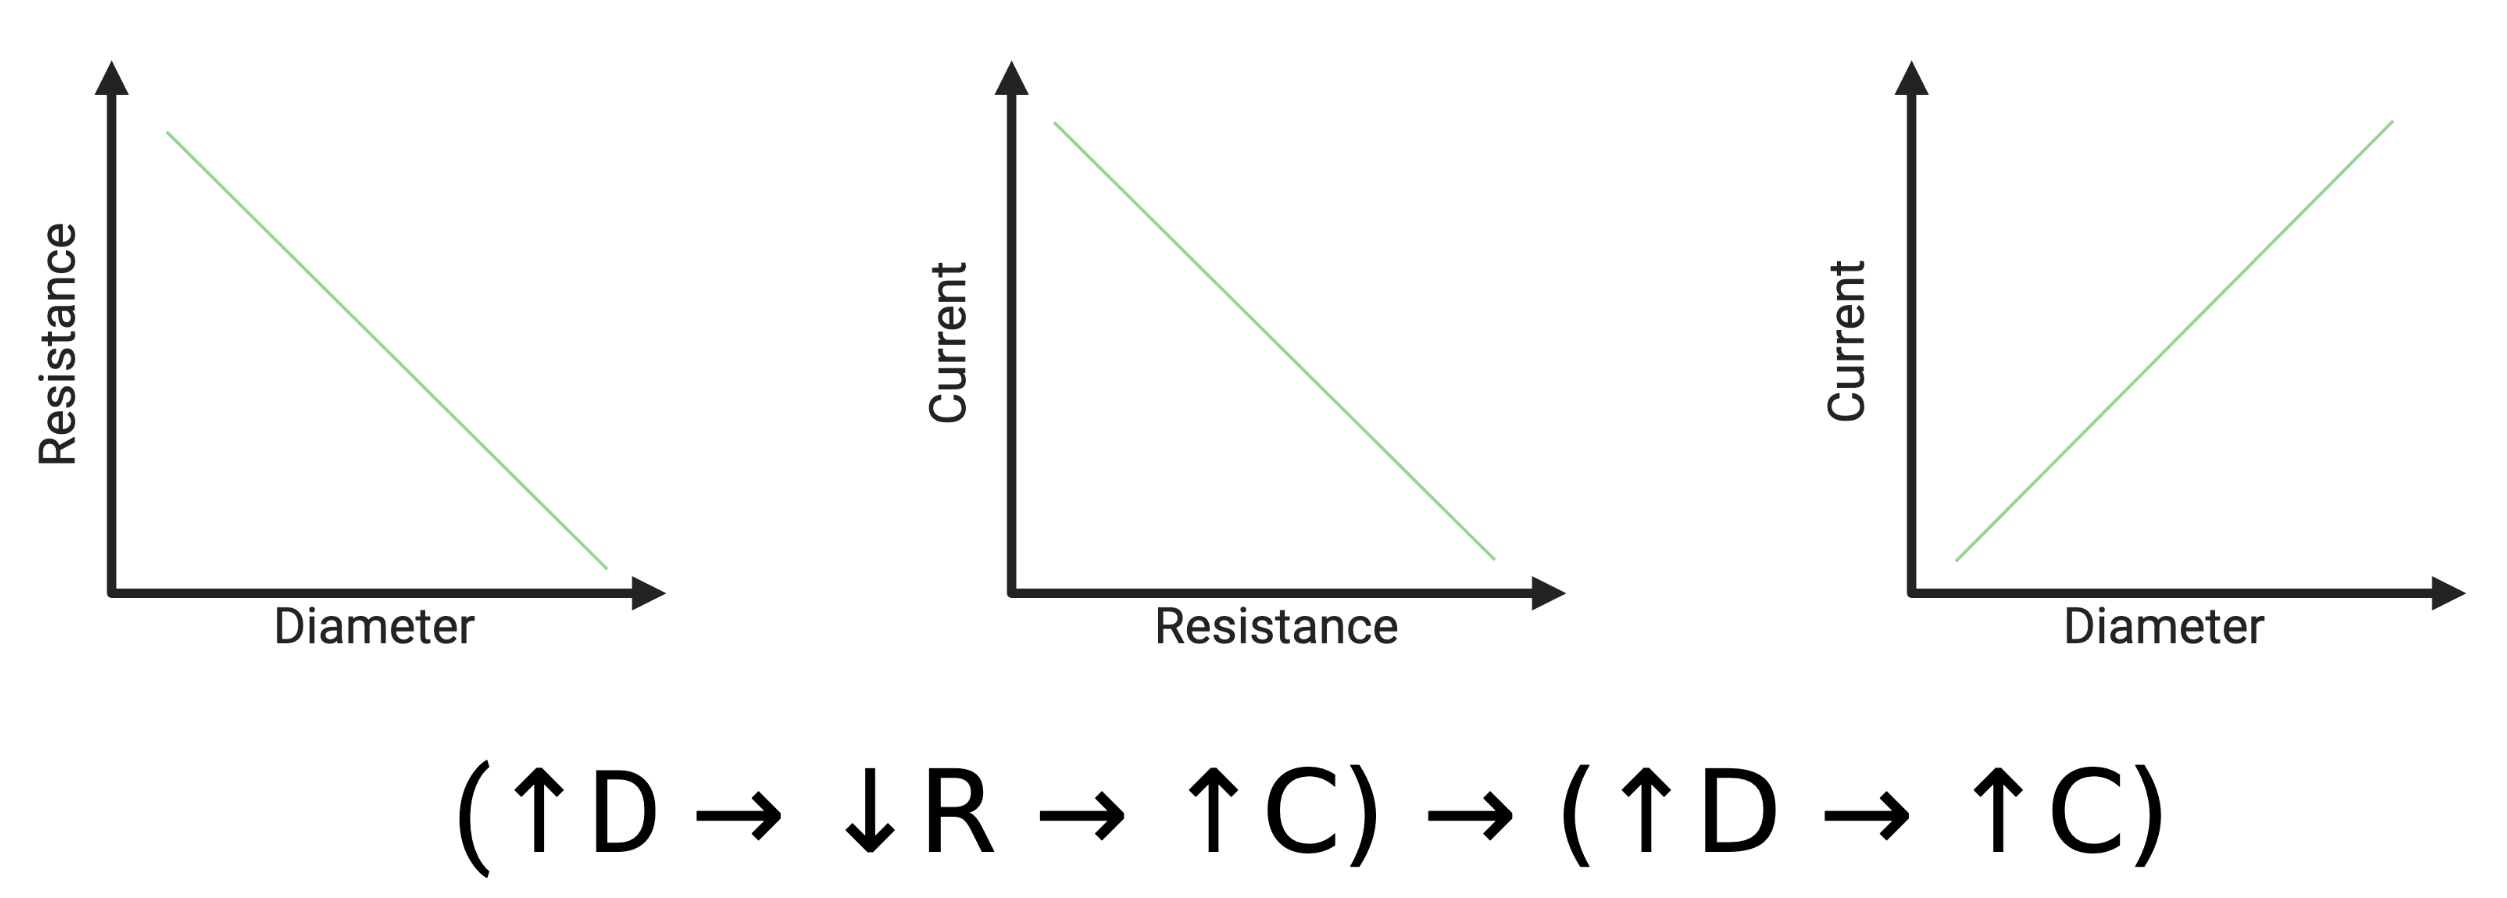
\includegraphics[width=1\linewidth]{./figure/Current_Resistance.png}
    \caption{Relationship between Diameter, Resistance and Current \footnotesize{(Created in BioRender.com)}}
    \label{fig:Current_Resistance}
\end{figure}

Estimated NCVs for three nerve fiber types are presented in Table \ref{table:NCV}. The $\alpha$-motor neuron has the highest NCV. The variation in diameter in the $\alpha$-motor neuron is explained by the motor unit types with the fast (FF) motor units innervating the FG fibers having the larger diameter ($\simeq 22 \mu m$) on the higher end for NCV ($\simeq 120 m \cdot s^{-1}$), and the S motor units with the small diameters ($\simeq 12 \mu m$)and the lower end of NCV ($\simeq 70 m \cdot s^{-1}$) (and FR motor units innervating FOG somewhere in the middle).  The terms fast and slow for the $\alpha$-motor neurons of motor units are relative to one another. It is clear in Table \ref{table:Innervation_Ratios} that both fast and slow $\alpha$-motor neurons are faster than the other neurons listed. They are faster due to both diameter (as compared to $\delta$-sensory neurons) and additionally myelination (as compared to C sensory neurons).

\begin{table}[h!]
\centering
\begin{tabular}{||c c c c ||} 
 \hline
Nerve Fiber & Diameter (\mu m) & NCV ($m \cdot s^{-1}$) & Function \\ 
 \hline\hline
 $\alpha$-motor & 12-22 & 70-120 & motor \\ 
 $\delta$-sensory & 1-5 & 12-30 & sharp pain \\
 C & 0.5-1.2 & 0.2-2 & dull pain \\ [1ex] 
 \hline
\end{tabular}
\caption{NCV for different nerve fiber types. Note: C fibers are unmyelinated, whereas $\alpha$-motor and $\delta$-sensory fibers are myelinated. Therefore, C fibers have a larger drop in NCV than would be estimated just from diameter. \footnotesize{Data from \cite{feher_quantitative_2017}}}
\label{table:NCV}
\end{table}

A fast $\alpha$-motor neuron has a larger diameter and myelin (structure) which both contribute to the NCV (function). Since the neurons of slow motor units are also myelinated the primary structural differentiation between fast and slow motor unit neurons are their size (larger diameters in fast motor unit neurons). Structurally, these larger neurons also innervate a higher number of muscle fibers. In mammalian muscles the IR for FF motor units is approximately twice (2x) that of S motor units, but this is an estimate that varies considerably between muscles (range from 1.1x to 3x greater than S motor units) \cite{bodine_maximal_1987}. 

A consequence of a larger neuron is that it requires more CNS excitation to become excited (excitation inertia). Excitation inertia has to do with how many ligand voltage gated channels must be opened before the threshold potential is reached. The larger (and thus faster) neuron has more excitation inertia. Fast $\alpha$-motor neurons are larger. While fast, they take more excitation to be excited. This is an important feature for motor unit recruitment and the size principle of recruitment order covered later in the chapter.

\paragraph{A note on motor unit and muscle fiber integrity}
Fast (larger) and slow (smaller) $\alpha$-motor neurons play a role for motor unit and muscle fiber integrity. The narrative of this chapter is that there is coherence between the neuron doing the excitation, and the muscle fibers being excited so that they can be activated. The neuron excitations play a critical, causal, role in determining the type of muscle fiber \cite{buchthal_motor_1980}. It is not a coincidence that faster and larger motor neurons innervate faster and larger muscle fibers. Studies using electrical stimulation and crossover (changing which neurons innervate which muscles), many muscle fiber characteristics change from slow to fast or from fast to slow. These experiments conclude that there is plasticity at the level of muscle fiber type with such experimental manipulations, and that this plasticity is related to the differences in electrical (not chemical) stimulus. The challenge to anyone wishing to alter their fiber type dominance is finding a way to  tap into the plasticity of the neurons.\footnotemark\footnotetext{Certain characteristics such as myosin and myosin ATPase isoforms rely on gene expression (one isoform is expressed or the other is expressed) and therefore may provide a limit to how much, or how many, muscle fibers have this plasticity.}

\paragraph{Summary of Fast \& Slow $\alpha$-Motor Neurons}
The functional characteristics that make the fast $\alpha$-motor neuron of the fast motor unit fast as compared to the slow classification are a higher NCV and a higher excitation frequency. The predominant structural difference that leads to these functional differences is the size of the neuron (larger, larger diameter). These structural and resultant functional differences fit on a spectrum that, in Table \ref{table:NCV}, result in a wide range of neuron diameters. These neuronal excitation characteristics innervate, and actually contribute to, coherence between the neuron and the muscle fibers of the motor unit.


\paragraph{Fast \& Slow Muscle Fibers}

The functional characteristics of muscle fibers that make them fast vs. slow include both structures related to excitation-activation coupling as well as structures related to activation (crossbridge kinetics). 

For muscle fibers in a fast motor unit to respond to the faster and higher excitation frequency of the neurons they require a well developed T-tubule and sarcoplasmic reticulum (SR) system. The SR and T-system of fast fibers can have up to three times the volume of slow fibers. This allows fast motor units to convert the higher frequency of nerve excitation into a higher frequency of muscle fiber activation.

With a higher frequency of muscle fiber activation there must be structural changes that also allow for faster crossbridge kinetics, otherwise the faster activation (faster release and update of $Ca^{2+}$ for example) would not result in faster twitches. The crossbridge kinetic structural changes tend to be discrete rather than on a spectrum.\footnotemark\footnotetext{By discrete we mean that there are no intermediate or transition steps between the structure. This is compared to changes such as the size of a SR or the diameter of a neuron or the number of ACh receptors at a NMJ where there can any number of transitional steps.} Fast fibers express an isoform of the protein myosin (particularly the heavy chain) and the enzyme (also a protein) myosin ATPase (responsible for hydrolyzing ATP on the myosin head). The combination of these two expressions allow for faster crossbridge kinetics (cycling through the sliding filament model) which leads to slightly more tension at the level of the sarcomere and a higher velocity for shortening \cite{larsson_maximum_1993, schiaffino_molecular_1996}. Therefore, when isolated or when either of these types of fibers dominate in a particular muscle, the force-velocity curve is shifted upward in fast as compared to slow motor units, with fast (FF) motor units having a higher velocity for any given force, and a higher force for any given velocity. 

These differences result in higher specific tension ($T_s$) in fast muscle fibers. $T_s$ refers to the tension developed per sarcomere or, more commonly considered, tension developed per unit of cross-sectional area. Since there are more muscle fibers in fast motor units means there are more sarcomeres and a greater cross sectional area, the $T_s$ makes the tension of a motor unit relative to its cross sectional area to allow comparison that avoids the confounding effect of greater cross sectional area.

The molecular (signal transduction) events that lead to the expression of myosin and myosin ATPase isoforms have not yet been completely uncovered.\footnotemark\footnotetext{Though, the author (SC) is still reading about the possibilities.} It is assumed that, due to the plasticity of muscle fiber types reported in experimental conditions, at least some muscle fibers retain the ability to express either isoform and that there exists a molecular mechanism that can theoretically be switched \cite{schiaffino_molecular_1996}.

\paragraph{Summary of Fast \& Slow Muscle Fibers}
The functional characteristics of muscle fibers for fast motor units allow for faster excitation-activation coupling and faster crossbridge kinetics. The structural characteristics that enable these include a higher volume of T-tubules and SR (for activation) and an isoform of myosin and myosin ATPase (for crossbridge kinetics). These changes result in an upward shifted force-velocity curve for fast motor units as compared to slow motor units (Figure \ref{fig:fiber_type_FV}). 

\begin{figure}[h]
    \centering
    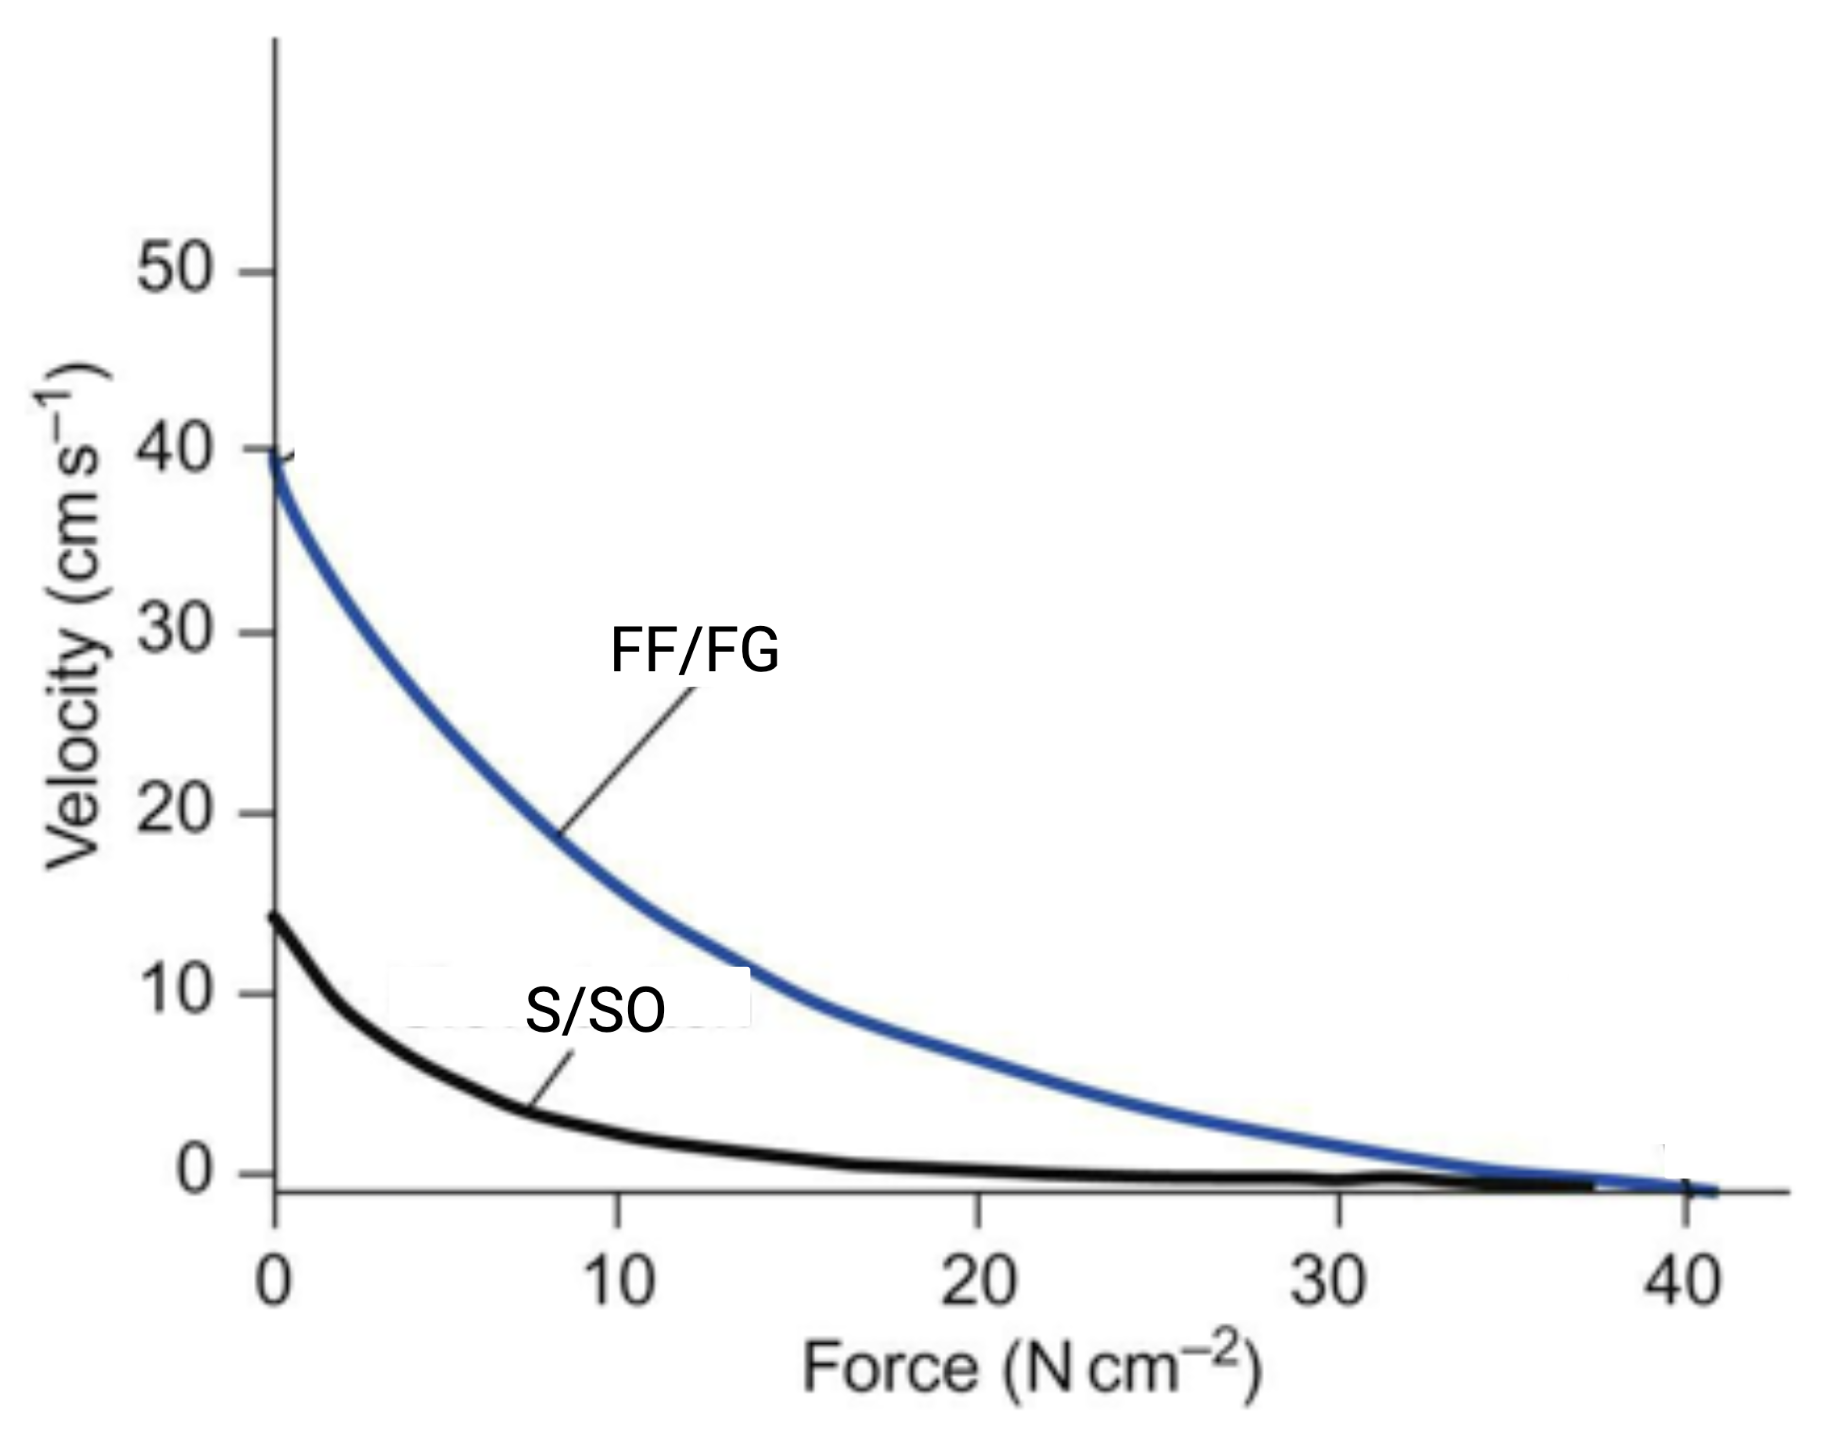
\includegraphics[width=1\linewidth]{./figure/fiber_type_FV.png}
    \caption{Force and Shortening Velocity of FF/FG and S/SO Motor Units \footnotesize{(Created in BioRender.com, Modified from \cite{feher_quantitative_2017})}}
    \label{fig:fiber_type_FV}
\end{figure}


\section{Motor Unit Twitch \& Tetany}

A single excitation of a muscle fiber produces enough activation to create a twitch, making a twitch the fundamental unit of active tension in the muscle fiber. The concept of a muscle fiber twitch is scaled up to a motor unit twitch. A muscle fiber twitch is the fundamental unit of active tension, a motor unit twitch is the fundamental unit of movement.\footnotemark\footnotetext{Just a note that by "unit" we don't mean unit as in a unit of measurement. Other words for how we are using the word unit may be "element" or "atom" or "particle".} Movements are created by muscle \textit{in situ}, and this means muscle fiber excitations and twitches occur in response to motor unit excitations, and the active tension developed by muscles that results in movement are based on motor unit twitches. Motor units have fidelity. When the neuron of a motor unit is excited all of the muscle fibers of the motor unit are excited. Recall from the data in Table \ref{table:Innervation_Ratios} that for the gastrocnemius this means a motor unit twitch includes approximately 1720 muscle fiber twitches. The fibers that are parallel increase the cross sectional area (A) and the tension.

\subsection{Motor Unit Type - Twitch \& Tetany Characteristics}

The three motor unit types display different twitch tension, twitch time and fatigue index (See Table \ref{table:Motor_Unit_Types}). These measurable functional characteristics are the result of the structural differences of both the motor unit neuron and the associated muscle fibers discussed in the previous section.

\begin{table}[h!]
\centering
\begin{tabular}{||c c c c||} 
 \hline
 Motor Unit Type & Twitch Tension & Twitch Time & Fatigue Index \\ [0.5ex] 
 \hline\hline
 Fast-Fatigable (FF)  & High & Fast & Low \\ 
 Fast-Resistant (FR)  & Moderate & Fast & Moderate \\
 Slow (S) &  Low & Slow & High \\ [1ex] 
 \hline
\end{tabular}
\caption{Motor Unit Types}
\label{table:Motor_Unit_Types}
\end{table}

\paragraph{Twitch Time}
Twitch time refers to the total time of the twitch with includes its upslope, time at peak or plateau, and time for downslope. A FF motor unit has a fast rise, short lived peak, and fast downslope. An S motor unit has a slower rise, longer plateau, and slower downslope. These characteristic curves (See Figure \ref{fig:mu_twitch}) contribute to the excitation frequency required for achieving tetany in the different motor unit types. An S motor unit can achieve tetany with an excitation frequency of 20-30 Hz since the twitches last longer and fuse (summate) more easily. A FF motor unit requires a higher frequency (80-100 Hz) to achieve tetany. 

\begin{figure}[!ht]
    \centering
    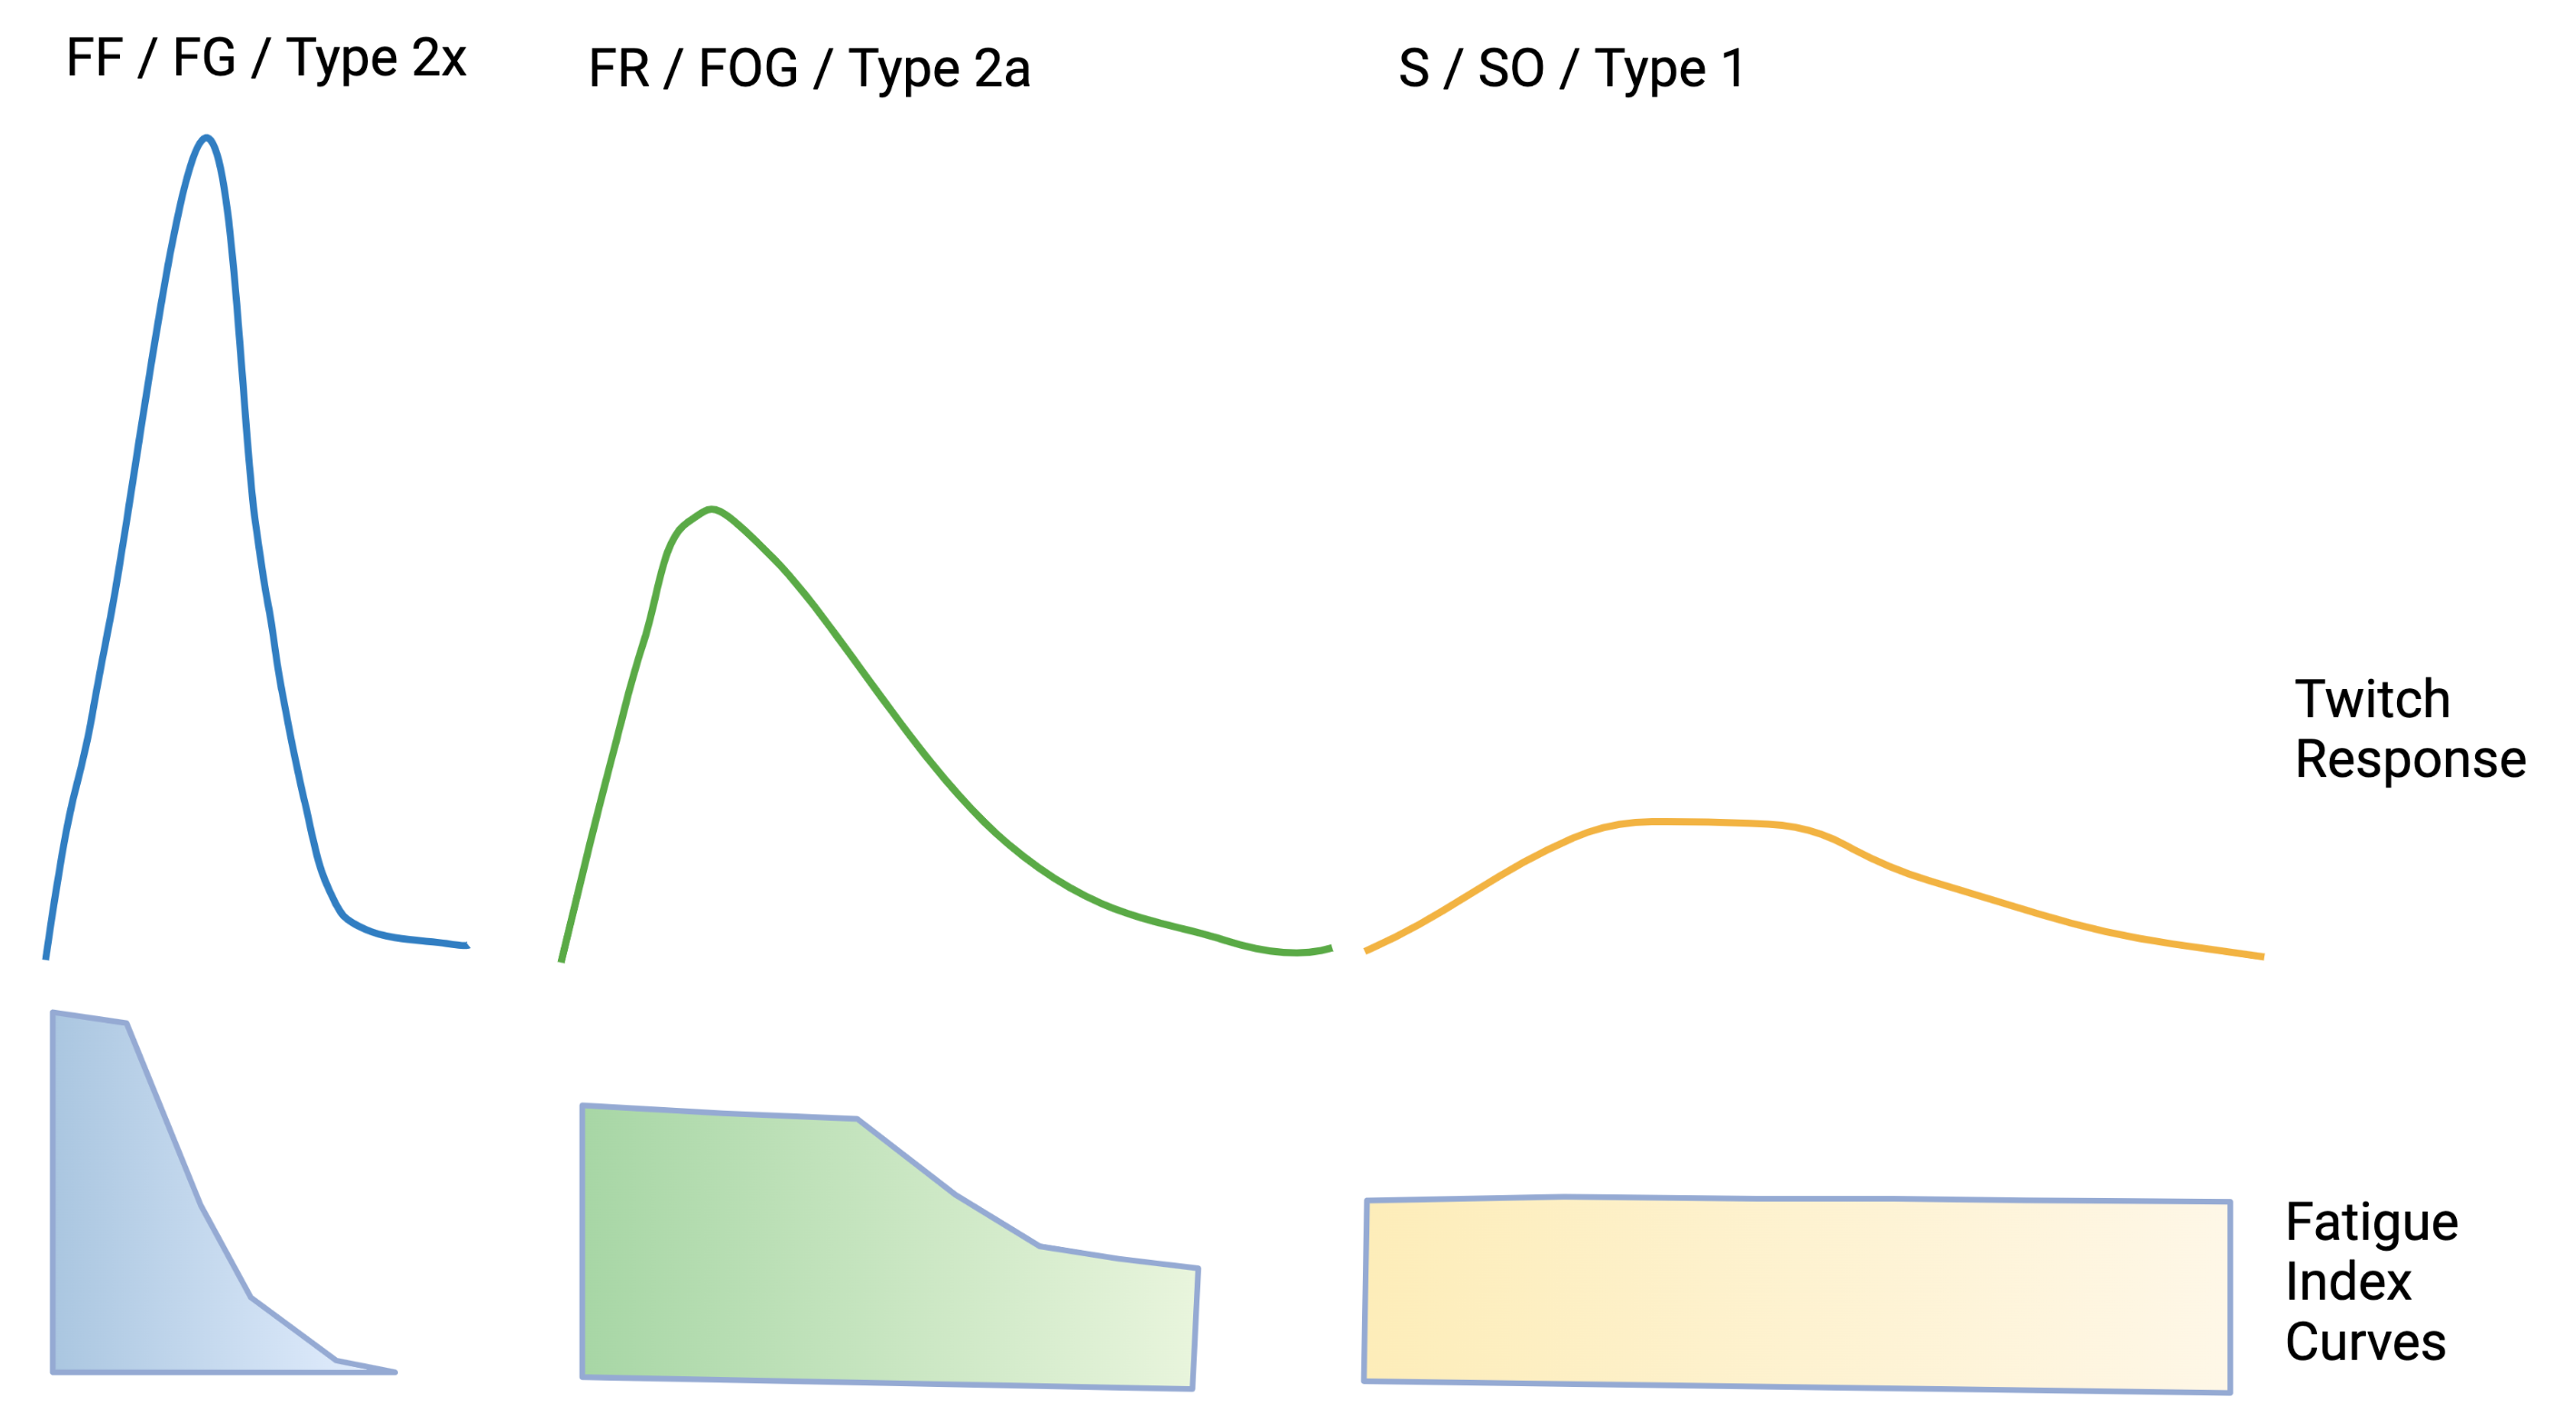
\includegraphics[width=1\linewidth]{./figure/mu_twitch.png}
    \caption{Motor Unit Twitch Characteristics \footnotesize{(Created in BioRender.com, Modified from \cite{jones_skeletal_2006}})}
    \label{fig:mu_twitch}
\end{figure}

\paragraph{Twitch Tension}
Twitch tension refers to the measurable force of a the tension developed during a twitch. Since tetany includes a summation of the twitches, a higher twitch tension results in a higher tetanic tension as well. Twitch tension is highest in the FF motor units for three reasons. First, these motor units have the highest number of muscle fibers (N, which is directly related to innervation ratio (IR)). Second, these motor units have, overall, a higher cross sectional area. Part of the larger cross area, but not all of it, is due to the higher number of fibers. The IR of a FF motor unit is approximately 2x higher than an S motor unit. However, the cross sectional area (A) is approximately 2.3x higher than an S motor unit \cite{bodine_maximal_1987, buchthal_motor_1980}. Third, these motor units have a slightly higher specific tension ($T_s$). Estimates are that the $T_s$ of FF motor units when tetanized is approximately $22 \ N \cdot cm^{-2}$ compared to S motor units approximately $17 \ N \cdot cm^{-2}$. Based on these estimates the $T_s$ of a FF motor unit is approximately 1.3x that of a S fiber. 

\paragraph{}

The tension of a motor unit twitch $T_{mu}$ is the sum of the motor units muscle fiber twitches $T_{mf}$. The equation:

\begin{equation}
    T_{mu} = N \cdot T_{mf} = N \cdot A \cdot T_s
\end{equation}

\begin{itemize}
    \item $N$ refers to the number of muscle fibers. This either is (for one motor unit) or can be estimated by (for an entire muscle) the innervation ratio.\footnotemark\footnotetext{$IR = \frac{N_{mf}}{N_{mu}}$ (Note, when there is one motor unit, $N = IR = N_{mf}$)}
    \item $A$ refers to the cross sectional area - an indication of how many sarcomeres are in parallel in the fiber.
    \item $T_s$ refers to the tension created for each unit of cross sectional area.
\end{itemize}

Using the above equation and estimates of FF motor units compared to S motor units we can derive an estimate of the FF motor unit $T_{mu}$ relative to the S motor unit. 

\paragraph{}
Assumptions:
\begin{itemize}
    \item FF motor unit IR, and therefore $N$ is 2x that of S motor units (more fibers)
    \item FF motor unit $A$ is 2.3x that of S motor units (greater cross sectional area)
    \item FF motor unit $T_s$ is 1.3x that of S motor units (higher tension per sarcomere)
\end{itemize}

An equation for the $T_{mu}$ for a FF compared to a S motor unit simply adjusts the variables based on a FF motor unit:

\begin{equation}
    T_{FF} = (N \cdot 2) \cdot (A \cdot 2.3) \cdot (T_s \cdot 1.3)
\end{equation}

This equation estimates that a FF motor unit can develop 6x more tension than an S motor unit. If based just on the number of fibers and the cross section area the estimate would be 4.6x. Therefore the number of fibers and the cross sectional area account for 76\% of the difference in tension between the FF and the S motor units. And the specific tension accounts for the remaining 24\%. Based on these estimates it is not surprising that differences in the specific tension between FF and S motor units is an area of controversy. When considering the likely variability between muscles, between samples, between mammalian species, differences as small as 1.3x are difficult to demonstrate \cite{lieber_skeletal_2010}. Some sources equate the $T_s$ between the two fiber types, $T_s \simeq 20 N \cdot cm^{-2}$ \cite{feher_quantitative_2017}, whereas others report them separately with albeit different estimates, FG $T_s \simeq 22 N \cdot cm^{-2}$, and SO $T_s \simeq 15 N \cdot cm^{-2}$ \cite{lieber_skeletal_2010}.

\paragraph{Fatigue Index}
Fatigue Index (FI) refers to how long tetany can be sustained for the FF, FR and S motor units. As Table \ref{table:Motor_Unit_Types} indicates, and Figure \ref{fig:mu_twitch} depicts the FF (fatigable) motor units have a low FI, whereas the S motor units have a high FI.

\subsection{Summary of Motor Unit Twitch \& Tetany}
The structural and functional differences between motor unit types result in expected differences in motor unit twitch and tetany characteristics. These differences lend themselves to the functional movement benefits of each type of motor units. FF motor units are optimized for fast, high force, high power - ballistic and temporary or intermittent movements. S motor units are optimized for slower, lower force and lower power - sustained, postural, stabilizing postures and movements. Further support of this story comes from how the motor units are recruited, that is, how tension is regulated.

\section{Active Tension Regulation}

Active tension is regulated through motor unit excitation. The two approaches include frequency summation (rate coding) of each motor unit and motor unit summation (recruitment) of more motor units. Both of these approaches start in the spinal cord with motor unit excitation.

\subsection{Motor Unit Excitation}

An $\alpha$-motor neuron, once excited, will release one neurotransmitter, ACh, at its axon terminal. ACh has one effect at the NMJ, creating excitatory micro-potentials on the motor end plate. In the CNS, more specifically for motor neurons in the spinal cord, competing neurotransmitters are released at synapses of the $\alpha$-motor neuron dendrites. The impact of these neurotransmitters can be excitatory or inhibitory. Since they occur after the synapse they are called excitatory post synaptic potentiations (EPSPs) or inhibitory post synaptic potentiations (IPSPs). Whether, and how frequently, an $\alpha$-motor neuron sends an excitation to the muscle fibers it innervates involves competition between the EPSPs and the IPSPs. For example, the IPSPs of certain protective reflexes associated with receptors in the muscle (see Golgi Tendon Organs below) can reduce the tension developed in a motor unit muscle fibers due to IPSPs lowering both the frequency of stimulation of a motor unit and the number of motor units recruited.

\subsection{Motor Unit Tetany - Frequency Summation}

Motor unit tetany involves the frequency of excitations. For any given motor unit, across all types, there is a range of excitation frequencies (rate coding) that can be used to vary the tension developed. It is estimated that frequency summation accounts for small fine tuning differences in tension. Frequency summation is not capable of resulting in large variations in tension in large part because it involves a set of muscle fibers that have a narrow functional frequency bandwidth. S type motor units can tetanize as low as 20 Hz, but don't develop any more force beyond perhaps 60 Hz (with a plateau occurring as low as 40 Hz). Similarly, FF motor units don't tetanize until they achieve upwards of 100 Hz and plateau at approximately 140-160 Hz. These differences, assuming linear increases in tension occur as frequency increases, represent a roughly 50\% increase in tension. If someone' grip strength is 100 pounds of force, then getting from 1 to 10 pounds of force requires a 10 times increase, getting from 1 to 100 pounds requires a 100 times increase. These increases in force cannot be accounted for by frequency summation. This has implications in situations discussed later which include a loss of motor units.

\paragraph{}

Frequency summation fine tunes and adjusts the tension in motor units but it is not capable of large fold changes in tension (or force). But, due to the role that excitation plays in motor unit tetany and the importance of tetany of motor unit muscle fibers for functional movements, the differences in the frequency of excitation to achieve tetany between the motor unit types is an important concept as we consider motor unit recruitment.

\subsection{Motor Unit Summation - Recruitment}

The primary way that muscle tension is regulated is through motor unit summation (recruitment). The recruitment of more motor units has the capability of greatly increasing the tension. From the example above, to go from 1 pound to a 100 pound hand grip requires the recruitment of few to perhaps all of the motor units involved in grip strength. Figure \ref{fig:Motor_unit_recruitment} depicts what happens when the three different motor units are recruited, first the SO fibers (S motor units), then the FOG fibers (FR motor units), and finally the FG fibers (FF motor units).\footnotemark\footnotetext{A future version of this figure will change upslope of these curves to represent the Twitch Time characteristics of the motor unit types).}


\begin{figure}[!h]
    \centering
    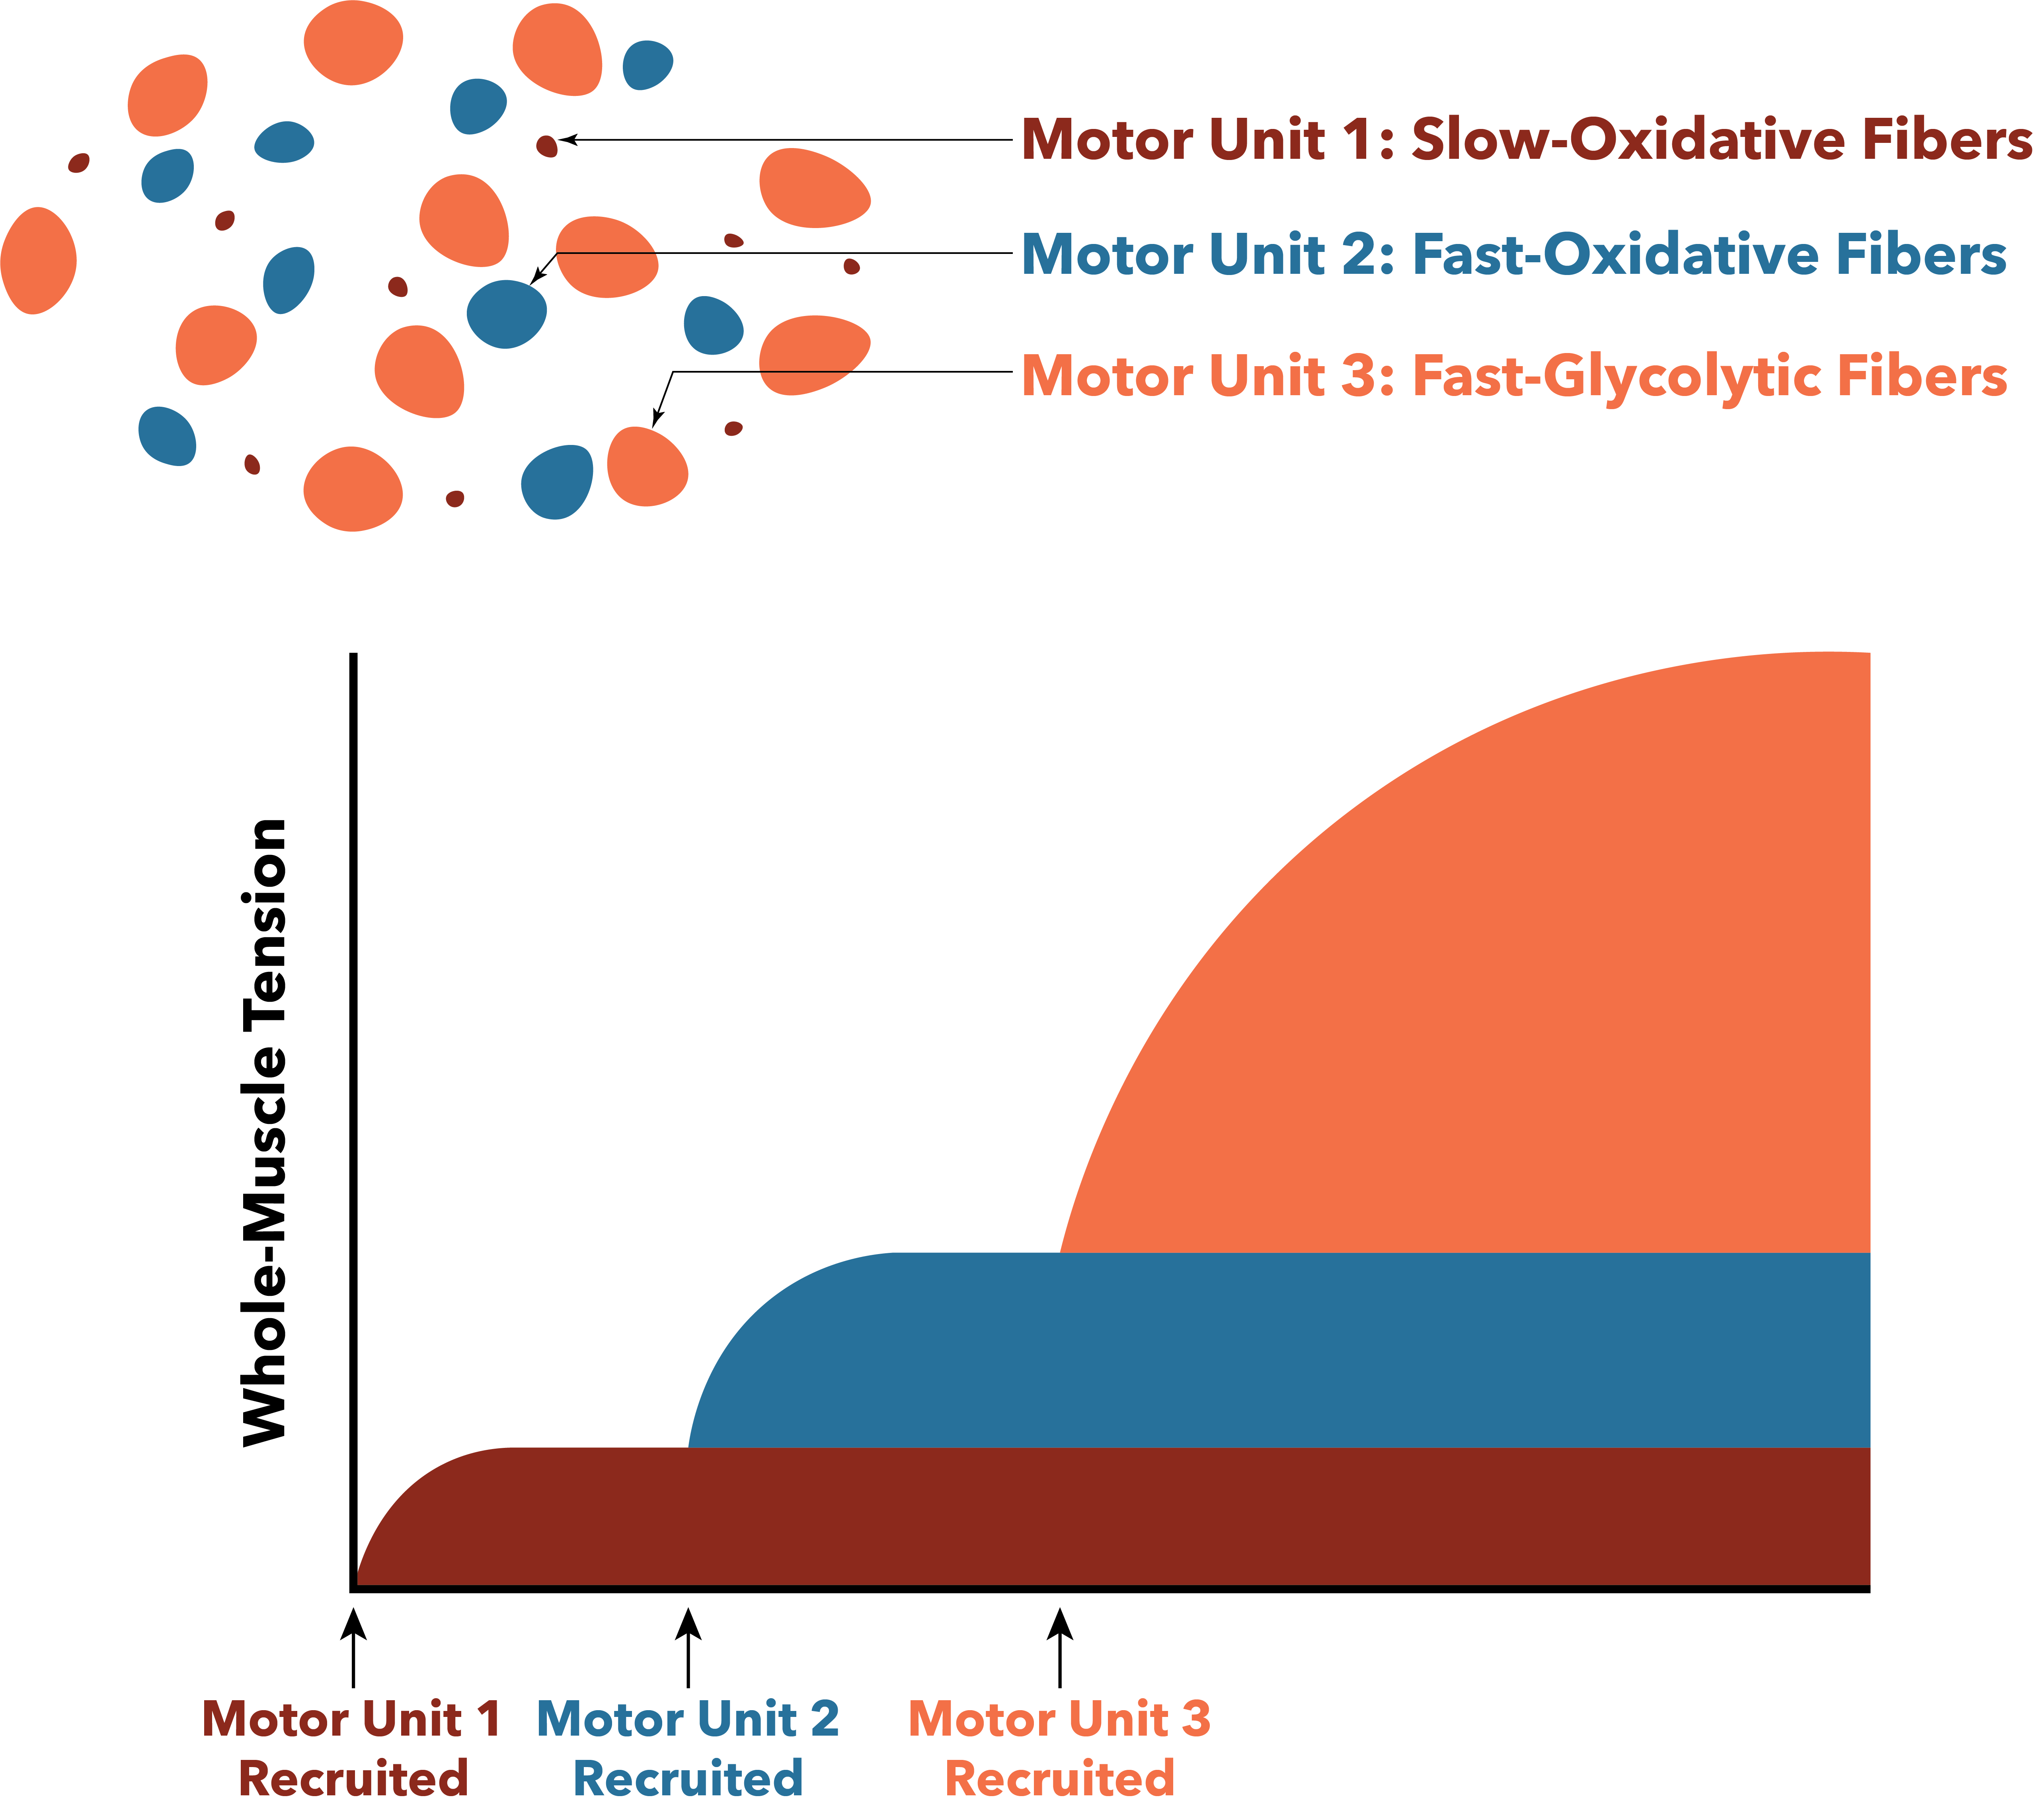
\includegraphics[width=1\linewidth]{./figure/Motor_unit_recruitment.png}
    \caption{Motor Unit Order of Recruitment \footnotesize{\href{https://commons.wikimedia.org/wiki/File:Motor_unit_recruitment.png}{Wikimedia Commons, CC BY 4.0})}}
    \label{fig:Motor_unit_recruitment}
\end{figure}

\paragraph{Size Principle of Motor Unit Recruitment}

The size principle of motor unit recruitment is based on the experimental observation that low tension requirements are met by first recruiting smaller motor units (S) with their associated SO fibers. As tension requirements increase the motor units recruited increase in size \cite{henneman_rank_1974}. This is due to two interrelated characteristics of the motor units themselves. First, smaller motor units require less excitation potentials to reach a membrane threshold potential. Lower CNS output into the region of the spinal cord (dorsal horn) with the dendrite pool of $\alpha$ motor neurons for a particular muscle first excites small dendrite membranes (they have less excitation inertia). As the CNS output increases in intensity, signaled as an increase in frequency of excitatory neurotransmitter impulses, there is an increase in excitation of the larger motor neurons. The second characteristic is that the larger motor neurons (FR and FF) require higher frequency excitations in order to achieve tetany.

\paragraph{Tension Developed during Motor Unit Summation - Recruitment}

Figure \ref{fig:n_motor_unit_recruitment} is a simulation based on the previously derived estimate that a FF motor unit generates 6x more tension than a S motor unit. This estimate accounts for the higher number of fibers, the greater cross sectional area of the fibers, and the greater specific tension of the fibers in an FF motor unit. Additional assumptions for this simulation include that the muscle has 100 motor units generating up to 100\% of of its maximal active tension; and that there are 20 S motor units, 20 S to FR transition motor units; 20 FR motor units; 20 FR to FF transition motor units; and 20 FF motor units. The S motor units each contribute 1 arbitrary unit (au) of tension, the FR motor units each contribute 3 au of tension, and the FF motor units each contribute 6 au of tension. The transition motor units are scaled linearly from 1 to 3, and from 3 to 6 in their respective transition zones. What is clear is that based on the order of recruitment (S to FF) there is an upward slope of tension with each new motor unit recruited. Jumps in tension as more motor units are recruited get larger as more motor units are recruited. Frequency summation tuning offers can further adjust these jumps. This tuning is more effective at lower tension with the small motor units since there are smaller jumps to accommodate.

\begin{figure}[!ht]
    \centering
    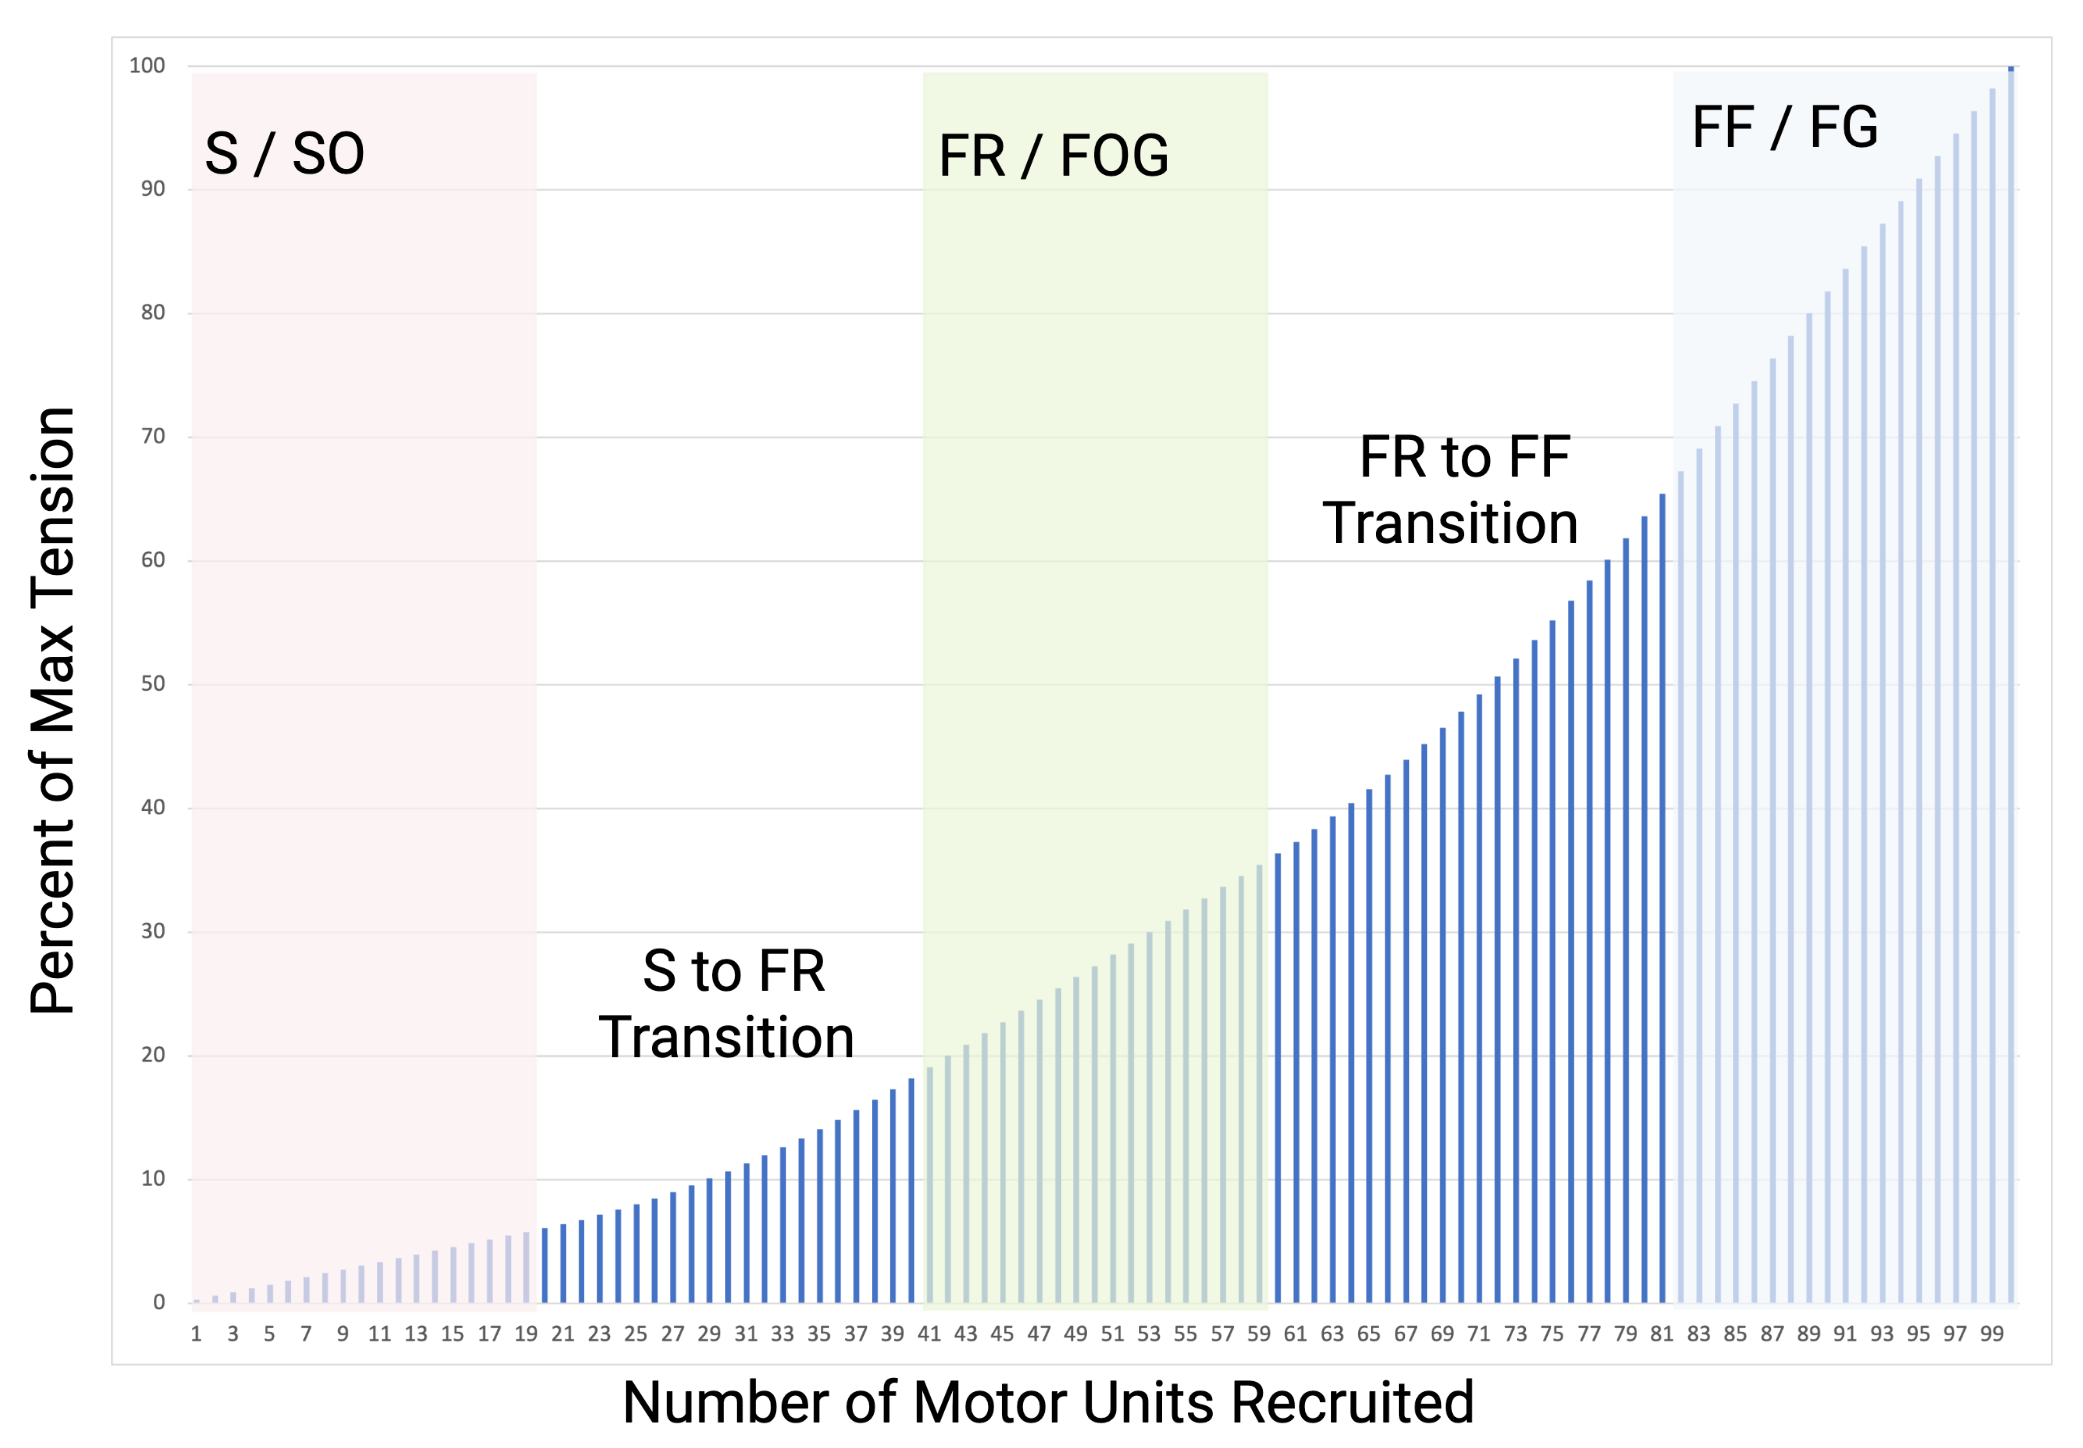
\includegraphics[width=1\linewidth]{./figure/n_motor_unit_recruitment.png}
    \caption{Simulation of Tension Developed during Motor Unit Summation - Recruitment (See text for simulation assumptions) \footnotesize{Created with Excel and BioRender.com})}
    \label{fig:n_motor_unit_recruitment}
\end{figure}

\paragraph{}

A commonly experienced consequence of the order of recruitment, that is clear in Figure \ref{fig:n_motor_unit_recruitment}, is that regardless of the muscle innervation ratio, there is less precision in tension regulation, and therefore less coordination and fine motor control when a muscle is being near maximal or maximally recruited. Muscles with lower IRs (such as the eye muscle described earlier with an IR of 5), will retain precision to a much higher level of tension, but it will still be reduced at higher tensions. If you have ever tried to fix your apple laptop and remove the small screws that require precision but a lot of force to remove, you understand the challenge of high tension precision.

\section{Regulatory Feedback}

It is estimated that between 40\% to 70\% of the nerves in a nerve bundle to a skeletal muscle fiber are $\alpha$-motor neurons (\underline{e}fferent nerves, \underline{e}xiting the spinal cord). The remaining axons are from sensor nerves (\underline{a}fferent nerves, \underline{a}ccessing the spinal cord). Regulation of tension is critically dependent on knowing whether the intention of tension is being met (whatever that intention may be) so that tension can be adjusted as necessary. Since neither motor control or neuroscience is a focus of this book (or course) this section is brief and focused on the muscle spindles and golgi tendon organs (GTOs) and how they influence tension regulation in the the spinal cord. 

\subsection{Muscle Spindles}

Muscle spindles are receptors that are excited when stretched and provide the central nervous system with information about muscle length and rate of stretching. With this information the muscle spindles are important contributors to proprioception (sensation and perception of position and movement). They are located within fascicles along side (parallel to) muscle fibers. It is conventional, once speaking of the muscle spindle, to refer to muscle fibers as extrafusal fibers (not part of the muscle spindle). The muscle spindles have both afferent and efferent innervation and their own small set of intrafusal contractile fibers. The intrafusal fibers are innervated by $\gamma$-motor neurons and allow the muscle spindle to adjust to the length of the muscle to remain sensitive to changes in length (See Figure \ref{fig:MuscleSpindle}). 

\begin{figure}[!ht]
    \centering
    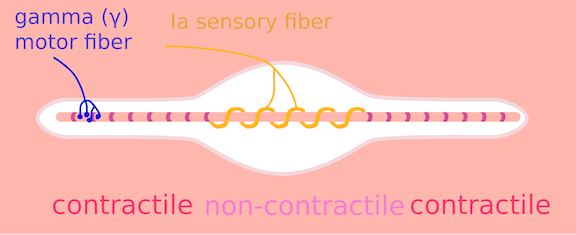
\includegraphics[width=1\linewidth]{./figure/MuscleSpindle.png}
    \caption{Muscle Spindle \footnotesize{\href{https://commons.wikimedia.org/wiki/File:MuscleSpindle.svg}{Wikimedia Commons, CC BY 4.0})}}
    \label{fig:MuscleSpindle}
\end{figure}

Afferent signals from the muscle spindles terminate at the spinal cord as well as higher up in the central nervous system for long loop reflexes and coordination (cerebellum) and the cerebral cortex (proprioception). The response of muscle spindles to a rapid increase in length (quick stretch) signals the dendrites of the $\alpha$-motor neurons of the agonist (same muscle that is being stretched) with excitatory post synaptic potentiations (EPSPs); and the dendrites of the $\alpha$-motor neurons of the antagonist (opposite muscles of those that are being stretched) with inhibitory post synaptic potentiations (IPSPs). Collectively these actions are referred to as the stretch reflex. If the stretch is quick enough and excites enough muscle spindles the EPSPs are sufficient to excite $\alpha$-motor neurons which provoke muscle excitation and activation. Testing stretch reflexes is an important component of a physical exam when the integrity of the $\alpha$-motor neuron, or any part of the sensory - motor reflex loop, is in question.

\subsection{Golgi Tendon Organs}

Golgi tendon organs (GTOs) are on the mostly tendon side of the transition space known as the musculotendinous junction. They are so close to muscle fibers that each GTO is connected in series with 5-20 muscle fibers. In this position the GTOs detect tension in muscle and tendinous fibers \cite{macefield_physiological_2005}. The GTO is excited by tension within the muscle fibers or tendon. Afferent impulses from the GTOs terminate in the spinal cord and cerebellum. GTO afferents in the spinal cord result in IPSPs of the agonist muscle. Inhibiting the agonist limits active tension as a protective mechanism.

\section{\textit{Clinical Physiology Connections}}

\subsection{Electromyogram (EMG)}

Each time a muscle fiber is activated it is caused by an excitation (action potential) from the nerve to the motor end plate, and along the sarcolemma of all the fibers that are innervated by that $\alpha$-motor neuron. Therefore, each muscle fiber activation is associated with an electrical signal. An EMG electrode near the fiber can record this electrical activity. The electrode can either be a small needle that acts as an antenna to record local electrical activity or a surface electrode (sEMG). If using a needle, the raw EMG signal can be used to accurately determine when a particular muscle is active (regardless of depth or size of the muscle). sEMG can be used to determine when a particular muscle is active when the muscle of interest is superficial and large enough to avoid cross talk at the sEMG electrode, but cannot be accurately used to determine specific activation of deep or small muscles. For example, sEMG just lateral to the spine cannot be expected to accurately identify activation of deep muscles such as the multifidi.

\paragraph{EMG quantification} It is difficult to quantify the activity of a muscle from a raw EMG signal. The EMG contains electrical signals from every muscle fiber in the vicinity of the EMG electrode which creates a very noisy signal (See Figure \ref{fig:EMG_ARV}). From the raw signal the Average Rectified Voltage (ARV) EMG can be computed. ARV is a time-windowed mean of the absolute value of the signal (turns all voltages into positive values). ARV is useful for further analysis such as recording the excitation patterns of a muscles that may include changes in excitation or as the first step towards more advanced analyses \cite{merletti_surface_2016}. The relationship between EMG activity and muscle tension is most valuable during isometric activation because the association between activation and tension changes with changes in length (length-tension relationship), and with different velocities (force-velocity relationship).

\begin{figure}[!ht]
    \centering
    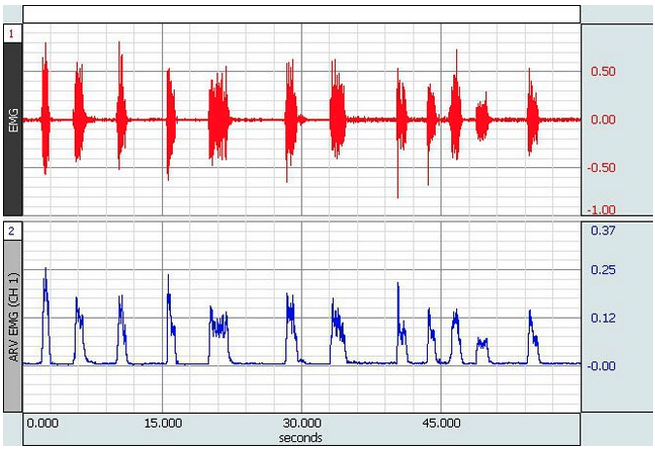
\includegraphics[width=1\linewidth]{./figure/EMG_ARV.png}
    \caption{Raw (upper) and ARV (lower) EMG Signals \footnotesize{Data collected using Biopaq acquisition hardware and Acknowledge software in the author's lab (SC)}}
    \label{fig:EMG_ARV}
\end{figure}

\paragraph{Biofeedback}

sEMG is a valuable form of biofeedback to indicate that a certain muscle has been activated. Commercially available devices provide visual or auditory signals so a patient can learn to activate a muscle. Common applications of the EMG for biofeedback is activation in the vastus medialis after anterior cruciate ligament surgery, or the lower trapezius during shoulder flexion or abduction.

\paragraph{Motor Unit Number and Size Indices (MUNIX \& MUSIX)}

The motor unit number index (MUNIX) and the motor unit size index (MUSIX) are based on sEMG data interpreted through a mathematical model to estimate an index of the number and size of functional $\alpha$-motor neurons for a muscle \cite{nandedkar_motor_2004}. MUNIX is not an absolute count of motor units, and MUSIX is not an absolute size of the motor units. But they do provide an estimate that correlates with other measures and they have reasonable reliability. Considering the test only takes 3-5 minutes per muscle, is non-invasive and relatively comfortable (as compared to other approaches), they have gained popularity in clinical neurology and neurophysiology. MUNIX is considered an effective bio-marker for assessing disease progression and an alternative clinical trial outcome for conditions associated with a decrease in motor units such as amyotrophic lateral sclerosis (ALS). It has also been proposed for use in the evaluation of peripheral neuropathies, particularly in demyelinating neuropathies with conduction block. While there have been less studies, MUNIX is starting to be evaluated in a variety of central nervous system disorders (such as spinal cord injury, stroke, and cerebral palsy \cite{fatehi_utility_2018}. 

A study of healthy individuals between 20 and 80 years of age demonstrated a reduction in MUNIX and MUSIX values with aging, particularly over the age of 60, indicating that they may be valuable biomarkers for research on the prevention and treatment of sarcopenia \cite{cao_reference_2020}. Sarcopenia is an age-related progressive loss of muscle mass and strength \cite{dao_sarcopenia_2020}. It is a type of muscle atrophy primarily caused by the aging process and certainly confounded by physical inactivity and malnutrition. Sarcopenia tends to result in a larger loss of FF motor units and FG (Type 2a) muscle fibers. If a loss of motor units is inevitable with aging, then healthy aging would strive for lifestyles that promote increasing MUSIX despite an inevitable decline in MUNIX. A consequence of this shift (reduced MUNIX and increased MUSIX) would be a reduction in muscle tension regulation. Therefore, the choice of lifestyle would need to consider the motor control (balance, coordination) capabilities in such individuals.

\subsection{Nerve Conduction Velocity (NCV)}

Nerve conduction velocity (NCV) refers to the time it takes for an excitation to travel a certain distance. It can be measured clinical with electrodiagnostic testing that includes EMG. A stimulus is presented proximally at a peripheral nerve and the distal muscle excitation (via EMG) or axonal excitation is measured.

The tight regulation of active tension for coordinated movement requires fidelity in the signals coming from the central nervous system.\footnotemark\footnotetext{Fidelity in this context means that intended signals are accurately sent where and when they are requested.} If the myelin sheath of an $\alpha$-motor neuron is damaged the NCV is reduced. If the NCV is reduced then the ability to activate muscles with high fidelity signals is impaired resulting in delays in the generation of active tension, limiting the ability to increase active tension when needed. These changes occur for two reasons, first, limitations in frequency summation, and second, limitations in motor unit summation. This is precisely what happens in peripheral demyelinating diseases such as Guillain-Barre syndrome, Chronic Inflammatory Demyelinating Polyradiculoneuropathy, and Anti-Myelin Associated Glycoprotein Neuropathy. The demyelinating disease known as Multiple Sclerosis (MS) also impairs signal fidelity, however, it is a central nervous system condition. Therefore, in MS the loss of signal fidelity does not directly alter the peripheral NCV, it impairs central NCV which interrupts signals that excite the motor unit dendrites in the spinal cord which contributes to a more complicated, nuanced and variable clinical presentation in terms of the impact it can have on motor function such as coordination.


\section{Summary \& Next Step}

Motor units connect the central nervous system to muscle fibers. Varying the frequency of excitation and the number of motor units excited allows the CNS to vary the active tension provided by a muscle. Tight regulation of this active tension is required for motor control. There are three accepted classifications of motor units and they correspond to three accepted accepted classifications of muscle fibers. The structural characteristics of these motor units and muscle fibers are related to distinct functional characteristics in twitch and tetany. Recruitment of motor units is the primary mechanism for varying tension with variations in the frequency of excitation providing a small range of tension variation that allows for fine tuning the nearly continuous range of possible tensions. Muscle spindles and golgi tendon organs provide the CNS with feedback about muscle tension, stretch and length. EMG can capture valuable information about motor unit and muscle excitation as well as the determination of NCV. The next chapter expands on the metabolic characteristics of muscle fibers and the impact muscle energetics has on function as well as the demands that muscle energetics places on other body systems.

\printbibliography[heading=subbibintoc]
% !TEX root = ../notes_template.tex
\chapter{Muscle Energetics}\label{chp:energetics}
Updated on \today
\minitoc

Muscles transform chemical energy into mechanical energy. The chemical energy utilized in this transformation is ATP. However ATP is not ingested and then circulated through the body to the cells. It is present in the cells in small quantities and regenerated in the cells at a rate that approximates its rate of utilization. The primary utilization of ATP in the muscle cell for active tension occurs when it is hydrolyzed by myosin ATPase during crossbridge cycling. The change in shape of the myosin head is potential mechanical energy that becomes kinetic mechanical energy during crossbridge activation. Muscle excitation and activation requires ATP in two other key steps. The $Na^+ / K^+$-ATPase pumps to establish the resting membrane potential, and the $Ca^{2+}$-ATPase pumps to return $Ca^{2+}$ into the sarcoplasmic reticulum. In addition to these clear ATP needs for excitation, activation and tension the muscle fibers require ATP for for membrane transport and synthesis of chemical compounds. These maintenance energy needs are critical for cellular integrity. 
The chemical energy to regenerate ATP comes from food we ingest, digest, absorb and metabolize into substrates. The absorption of glucose can be directly utilized as a source of energy. All other substrates require metabolism, fatty acids, proteins, glycogen (stored form of glucose).
This chapter considers the rate and capacity of pathways to regenerate ATP in muscle cells. These pathways vary across a spectrum with rate of regeneration inversely related to capacity. They are all always being utilized to some extent during muscle cell energetic transformations. Structural variations that exist on a spectrum between muscle fibers result in functional variation in their ability to carry out these five pathways with a high degree of adaptability. Clinical physiology connections emerge based on an understanding of energetics, this chapter focuses on the implications of sarcopenia, the concept of fatigue, and the pathophysiological concepts of hypoxia, hypoxemia and ischemia.

\vspace{5mm}

\textbf{Objectives include:}
\begin{enumerate}
    \item Explain the factors underlying the storage, use and regeneration of ATP.
     \item Compare and contrast the energetic system pathways that transform macro nutrient substrates to ATP.
    \item Compare and contrast muscle fiber differentiation (types) based on energetic structures and resultant functional capacities.
    \item Provide examples of possible differences in muscle tension energetic characteristics and performance based on hypothetical changes to muscle fiber types or aspects of the energetic pathways.
    \item  Apply the concepts of mass balance, flow gradients, and energy to the analysis of patient/client problems related to the muscular system.
     \item Evaluate the reasons different energetic pathways are primary sources of ATP in different activities, and analyze the response to different activities based on the primary energetic pathway being used.
     \item Explain the implications of sarcopenia on muscle strength and endurance.
     \item Explain the concept of, and the energetic basis of, fatigue.
     \item Explain the energetic basis of hypoxia, hypoxemia and ischemia.
\end{enumerate}

\section{Energetic Transformation Overview}

Energetic Transformation is a slightly more explanatory way of describing what is commonly referred to as metabolism. Of course, there are many different types of energetic transformations occurring when considering all metabolism throughout the body. And not all metabolic reactions are specifically about the regeneration of ATP. Our focus is on energetic processes and pathways that transform substrate energy to regenerate ATP in muscle. Most of these processes and pathways occur in cells throughout the body.

Muscle fibers continuously utilize ATP. Resting utilization of ATP results in a steady demand for ATP which is met by an equal rate of ATP regeneration. The balance of demand and regeneration (supply) is regulated by the cell. The muscle fiber stores ATP at relatively low concentrations (5 $mmol \cdot L^{-1}$) \cite{feher_quantitative_2017, jones_skeletal_2006}. At rest there are low energetic needs (low ATP demand) so the tendency to store a small amount of ATP is not a problem. But muscle fibers can increase their energetic needs (rate of ATP utilization, demand) 60-100 fold during transitions from rest to high levels of tension. When ATP demand increases, supply (rate of ATP regeneration) must increase in response. Resting muscle has approximately 1 $mmol \cdot L^{-1}$ of ADP and 10 $mmol \cdot L^{-1}$ of $P_i$. Regulating the rate of ATP regeneration is based on maintaining this 5:1 ratio of ATP:ADP. When the muscle fiber starts to use more ATP the ratio drops and the rate of regeneration increases throughout all pathways until the ratio is reestablished. If it cannot be reestablished by increasing the rate of regeneration and the amount of ATP falls below the ATP demand, then whatever functions need ATP start to fatigue (fail to perform their act). 

There are two proposed reasons that ATP is not stored in large quantities. First, it is a heavy molecule. It is estimated that an individual regenerates their body weight worth of ATP \cite{tornroth-horsefield_opening_2008}. ATP is 507.18 g/mole. Whereas glucose is 180 g/mole and even fatty acids with up to 29 carbon chains and double bonds (high energy) have molar masses lower than ATP (less than 500 g / mole). Since mass (and weight) influence the energetic costs of movement then storing ATP is a less efficient approach to energy storage than storing glucose (as glycogen) and fatty acids (as adipose tissue). Second, ATP is a highly reactive molecule that triggers several cellular events by binding and hydrolyzing. Too much ATP being stored could cause "chaos" in cellular functions \cite{jones_skeletal_2006}. The implications of not storing ATP includes the continuous need to regenerate ATP at the rate it is being utilized while maintaining a reserve (surge) capacity.



\section{ATP Regeneration Pathways}

There are six ATP regeneration pathways in the muscle fiber. The myokinase pathway is briefly described as part of the immediate ATP/Phosphocreatine (PCr) pathway. The pathways are summarized in Figure \ref{fig:Energetics_Overview}. The rates and capacities of the pathways are later directly compared in Table \ref{table:ATP_Rates}. 


\begin{figure}[!h]
    \centering
    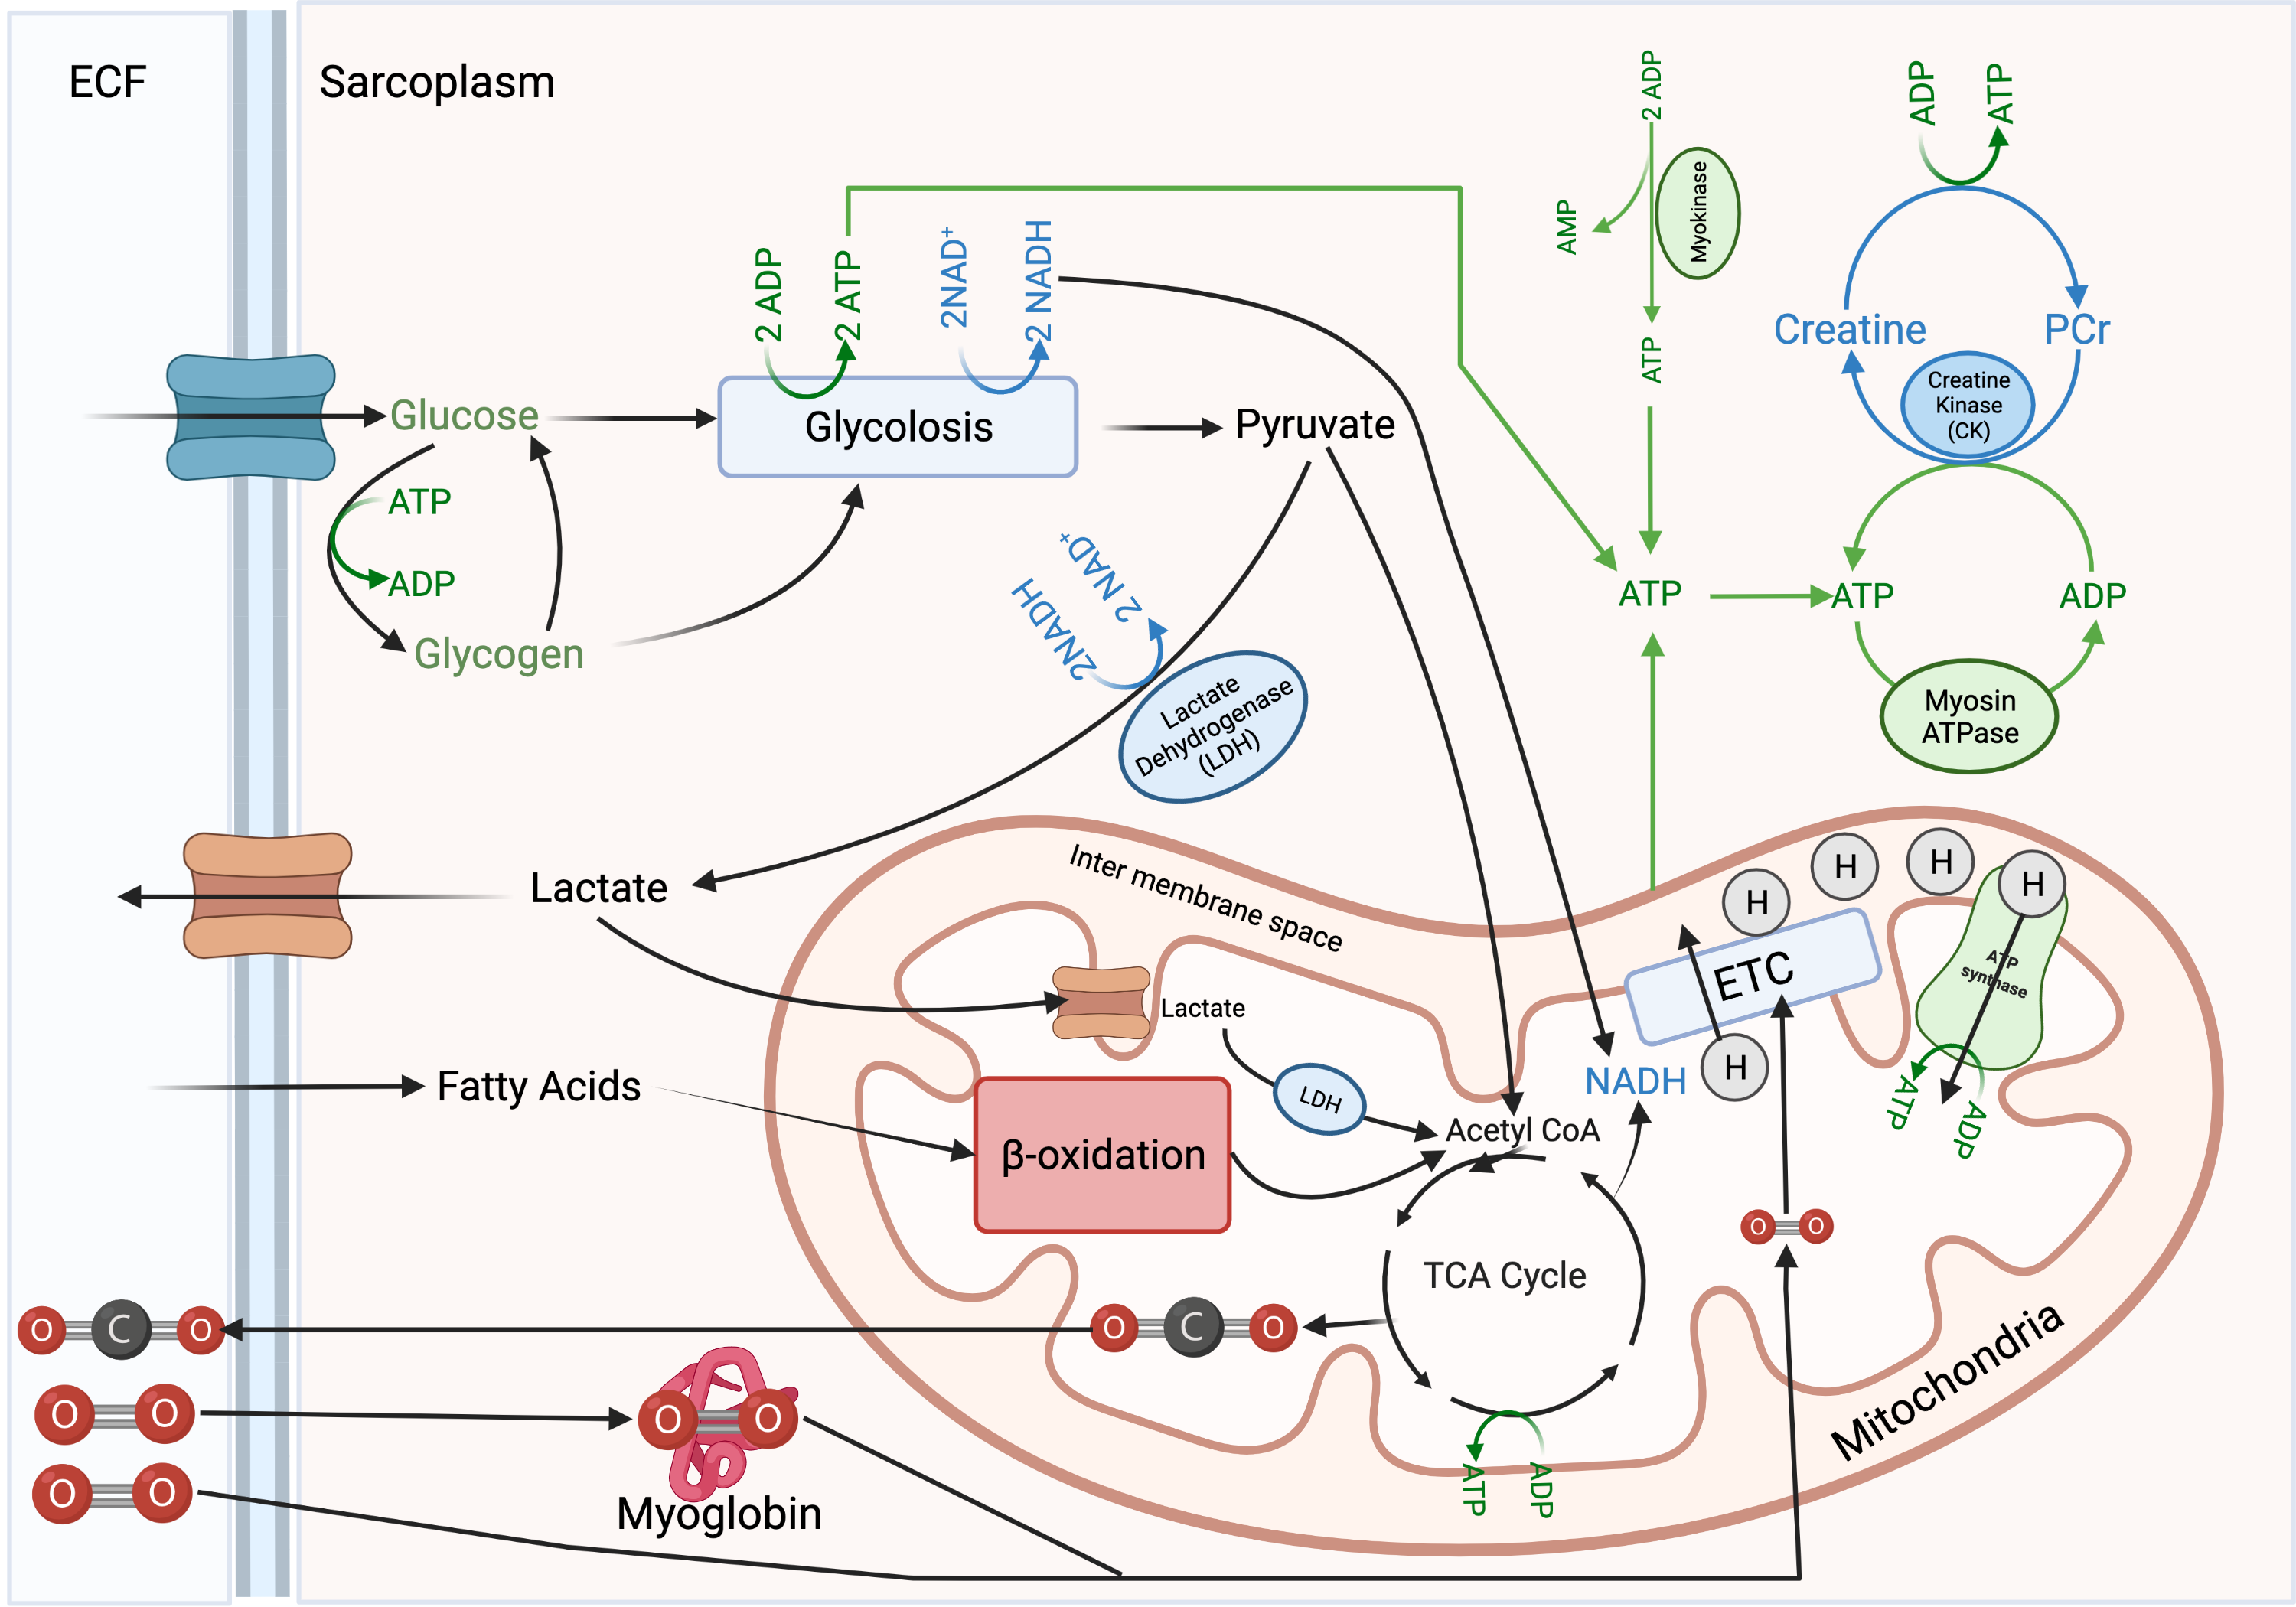
\includegraphics[width=1\linewidth]{./figure/Energetics_Overview.png}
    \caption{Overview of Energetic Transformation Pathways in a Muscle Fiber. The only pathway not explicitly included in this graphic is the pathway that starts with the breakdown of glycogen to release glucose into the blood which ultimately enters cells through the glut4 channel. This and other important metabolic processes and pathways in the liver are covered in Chapter \ref{chp:blood_nutrients}. (\footnotesize{Created with BioRender.com})}
    \label{fig:Energetics_Overview}
\end{figure}

Some of the pathways occur in the sarcoplasm (outside of the mitochondria, including PCr, Myokinase, Muscle Glycogen $\rightarrow$ Lactate Pathway). These pathways are not rate limited by the structural requirements of mitochondria.  Pathways occurring outside of the mitochondria do not involve cellular respiration and are referred to as anaerobic (not requiring $O_2$). The anaerobic pathways follow standard chemical substrate phosphorylation. The chemical reactions of these pathways are catalyzed by enzymes and regenerate ATP at high rates but low overall yield. The low yield is due to the fact that they tend to be self limiting. They either recycle existing energy and quickly exhaust their capacity (myokinase and PCr) or they create byproducts that inherently limit their process (the glycolytic process within the Muscle Glycogen $\rightarrow$ Lactate pathway). With either self limitation they can temporarily regenerate ATP at a higher rate than their support systems allow. They meet a particular need, provide a high rate of ATP regeneration, but fatigue quickly and must recover. Such work:recovery cycles are a recurring theme for the concept of fatigue.

Pathways occurring in the mitochondria involve cellular respiration and are referred to as aerobic (Muscle Glycogen $\rightarrow$ $CO_2$; Liver Glycogen $\rightarrow$ $CO_2$; Fatty Acid $\rightarrow$ $CO_2$ pathways). All pathways that produces Acetyl Co-A enter into the citric acid cycle (TCA, Kreb's Cycle). TCA contributes some ATP, but primarily contributes more $NADH$ and creates some $CO_2$ in the process. $NADH$ is utilized to generate large quantities of ATP by sending it through the Electron Transport Chain (ETC). The ETC utilizes $NADH$ to build a concentration and electrochemical gradient of H+ in the mitochondrial inter membranous space. ETC rate dependent on the availability of $O_2$ to accept the transported electrons in the final step. The energy of this gradient is pushed through ATP-synthase like water through a turbine at a dam. The reason there are fluctuating estimates on the number of ATP produced through aerobic pathways (oxidative phosphorylation) is that the ATP is produced by the function of a molecular machine, not with standard chemical substrate phosphorylation. 


\paragraph{There is no switch!}
There is no switch that turns on anaerobic energy transformation and turns off aerobic; or that turns on aerobic or off anaerobic. There are no exercises that are exclusively anaerobic or exclusively aerobic. A slow walk still utilizes anaerobic pathways. A heavy lifting session regenerates ATP and PCr utilizing the underlying continuous activity aerobic pathways. Dispel any notions that these socially constructed concepts entail an exclusive monopoly of energetic pathways to regenerate ATP. All energetics are on a spectrum. The primary demand for ATP during the slow walk are met by aerobic pathways, and the primary demands of the heavy lifting session are met by anaerobic pathways. But all ATP is ultimately regenerated by aerobic metabolism. It is this concept of meeting primary demands that has been utilized for the social construction of aerobic and anaerobic exercise and the misinterpretation that these are mutually exclusive pathways.

\paragraph{There is no ATP Debt}

There is no such thing as ATP debt. ATP utilization during crossbridge activation by myosin-ATPase is absolute. If there is not enough ATP there will be less crossbridges involved in generating active tension. The active tension cannot be generated with the energy for the tension paid back later. Either the pathways provide a way to regenerate the ATP at a rate needed for the demand, or the active tension is not generated as intended. The primary determinant - in a muscle fiber - of the rate of ATP utilization, and therefore need for regeneration, is the frequency of excitation - activation. The primary determinant - in an entire muscle - of the rate of ATP utilization, and therefore the need for regeneration, is the frequency excitation across all the motor units recruited. If the ATP is not regenerated at the rate it is being utilized, cellular functions do not occur. 

\paragraph{Energetic Pathways - Directed Graph}

Figure \ref{fig:energetic_paths} is a directed graph (DG) of the energetic pathways. Details are excluded. All models are wrong, some models are useful. This directed graph is useful for tracking the different energetic paths. This DG does not have clear boundaries for intracellular and extra cellular, or sarcoplasm and mitochondria spaces. A general pattern of the DG is that things entering the fiber come from the top or left of the graph, and things exit the fiber to the right. It is recommended that the reader compare and contrast Figure \ref{fig:Energetics_Overview} and \ref{fig:energetic_paths}. 

\begin{figure}[!h]
    \centering
    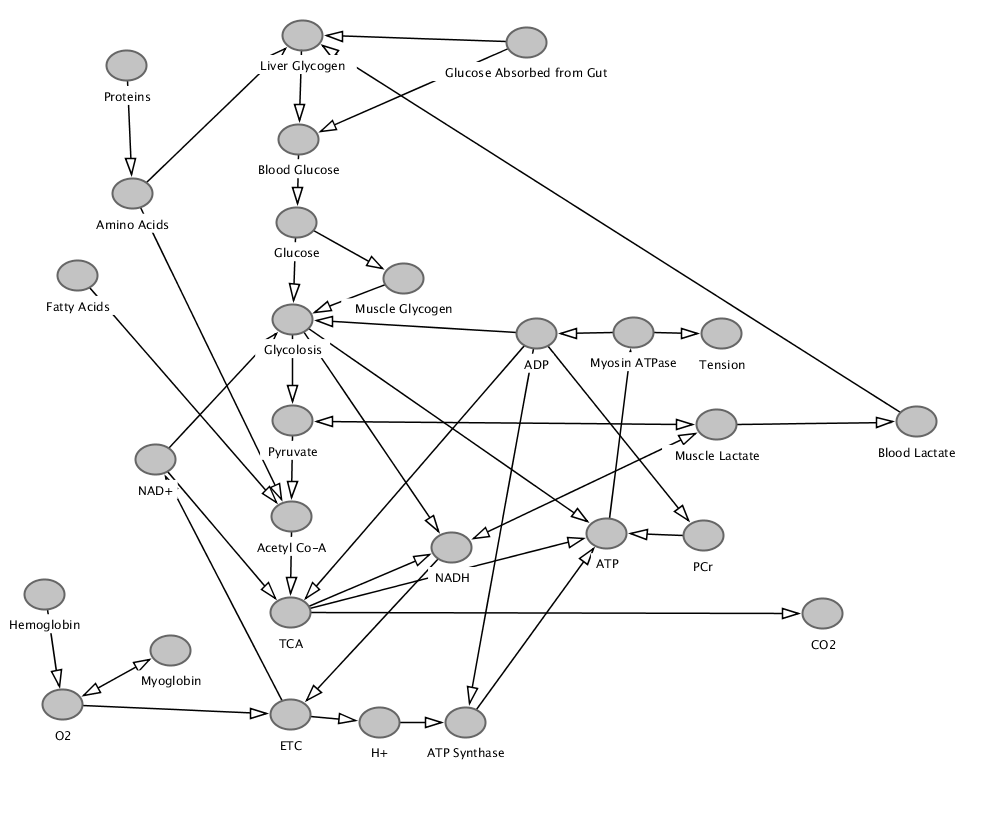
\includegraphics[width=1\linewidth]{./figure/energetic_paths.png}
    \caption{A directed graph (DG) of the energetic pathways (\footnotesize{Created with DAGitty.com and available for modifying at \url{http://dagitty.net/mZ_hp70}})}
    \label{fig:energetic_paths}
\end{figure}

% You are now registered as the owner of the saved graphical model available at: dagitty.net/mZ_hp70
% Please use the following password when modifying or deleting the model:
% yvrzZ9.U6d



\subsection{ATP / Phosphocreatine (PCr) (immediate) Pathway}

Creatine is synthesized in the liver, or ingested, digested and then absorbed from meat or ingested and absorbed from supplementation.\footnotemark\footnotetext{Creatine is a molecule that can be absorbed directly through the gut into the blood. Creatine supplementation will be a clinical connection in Chapter \ref{chp:blood_nutrients} on Visceral Support.} A high energy bond can form between creatine and phosphorous ($P_i$), forming PCr.

The reaction: $PCr \rightleftharpoons ATP$ is a reversible high rate reaction catalyzed by the enzyme creatine kinase (CK). The rightward reaction (PCr to ATP) regenerates ATP for cellular functions. At rest about 80\% of creatine is in the energized (PCr) state and there is approximately five times as much PCr than ATP (PCr:ATP ratio of 5:1) in a muscle fiber. Based on the weight and reactive volatility of ATP, PCr is provides a very important reserve of high energy phosphate bonds for ensuring the muscles ability to meet high energy demands, and even to smooth out transitions between lower and higher ATP utilization rates.\footnotemark\footnotetext{In a muscle fiber the primary determinant of ATP utilization is the frequency of activation which is directly proportional to frequency summation.} It is a stable and relatively light form of energy to store in the muscles.

PCr is considered an immediate source of ATP and the flux rate of PCr to ATP is determined by the ATP:ADP ratio. As ADP levels increase the rate of PCr to ATP reactions increase and will continue until PCr is expended or ADP drops to a normal level.

The maximum rate of $PCr \rightleftharpoons ATP$ is much higher than other pathways, upwards of 4.4 moles/minute of ATP. However, it is only capable of regenerating approximately 0.7 moles of ATP overall. Therefore, when working at maximum capability (rate of 4.4 moles/minute) it is sustained for 9.5 seconds (See the Summary of Max Rates of ATP Regeneration by Pathway in Table \ref{table:ATP_Rates}). This time estimate is dependent on the assumption of the max rate (4.4 moles/minute). Once the capacity of PCr to regenerate ATP is exhausted (fatigued) the muscle cannot continue to generate a tension that requires that rate of ATP utilization.

If a lower rate of ATP was being utilized, say 0.5 moles/minute, then PCr would be able to sustain ATP regeneration much longer. And since that rate of ATP utilization is lower than other pathways then PCr would continue to be regenerated by ATP coming out of the mitochondria. In this situation the need for ATP from PCr would not approach maximum because the aerobic pathways are contributing to the ATP regeneration.

Even though PCr is most often thought of as the source of ATP for high muscle tension activities, it also is the initial source of ATP for any changes in the rate of utilization of ATP because other pathways have a delay (when compared to PCr) in how quickly they can start regenerating more ATP. Therefore, PCr is the source of ATP for a sudden burst of tension such as that needed to increase pace during a run, or increase velocity of a movement. PCr ensures that ATP is regenerated at the rate needed during any transitions in the rate of ATP utilization. In this sense, it buffers differences between ATP demand and supply and thus allows smooth active tension transitions.

\paragraph{ATP-PCr Sarcoplasm Shuttle}
The PCr pathway is also utilized as a ATP transport mechanism throughout the sarcoplasm (ATP-PCr shuttle). There are substantial diffusion barriers in a muscle fiber due to the number of highly structured protein complexes. The mitochrondria are near the sarcolemma (along with the nuclei largely because the rest of the fiber is packed tightly with myofilaments). The diffusion of ATP from the mitochrondria to myosin-ATPase is challenging. PCr is diffused through the entire sarcoplasm and due to its rapid regeneration rate can easily shuttle (or pass) the energy of ATP through the sarcoplasm from just outside a mitochondria to near the myosin ATPase. During muscle activation when the rate of ATP use by the myosin ATPase increases the nearby PCr regenerate ATP and then that regeneration can propagate from all around the sarcoplasm, and from near the mitochondria, to shuttle ATP toward the myosin ATPase (See Figure \ref{fig:PCr}). This movement - either the diffusion of ATP directly or the use of an ATP-PCr shuttle - is based on an ATP flow gradient from the mitochondria (source) toward any steps utilizing ATP (sinks). The more ATP being utilized by the myosin ATPase, the $Na^+/K^+$-ATPase or the $Ca^{2+}$ ATPase the lower the concentration of ATP near those proteins (sinks) and the greater the diffusion, and shuttling, of ATP towards those locations.

\begin{figure}[h!]
    \centering
    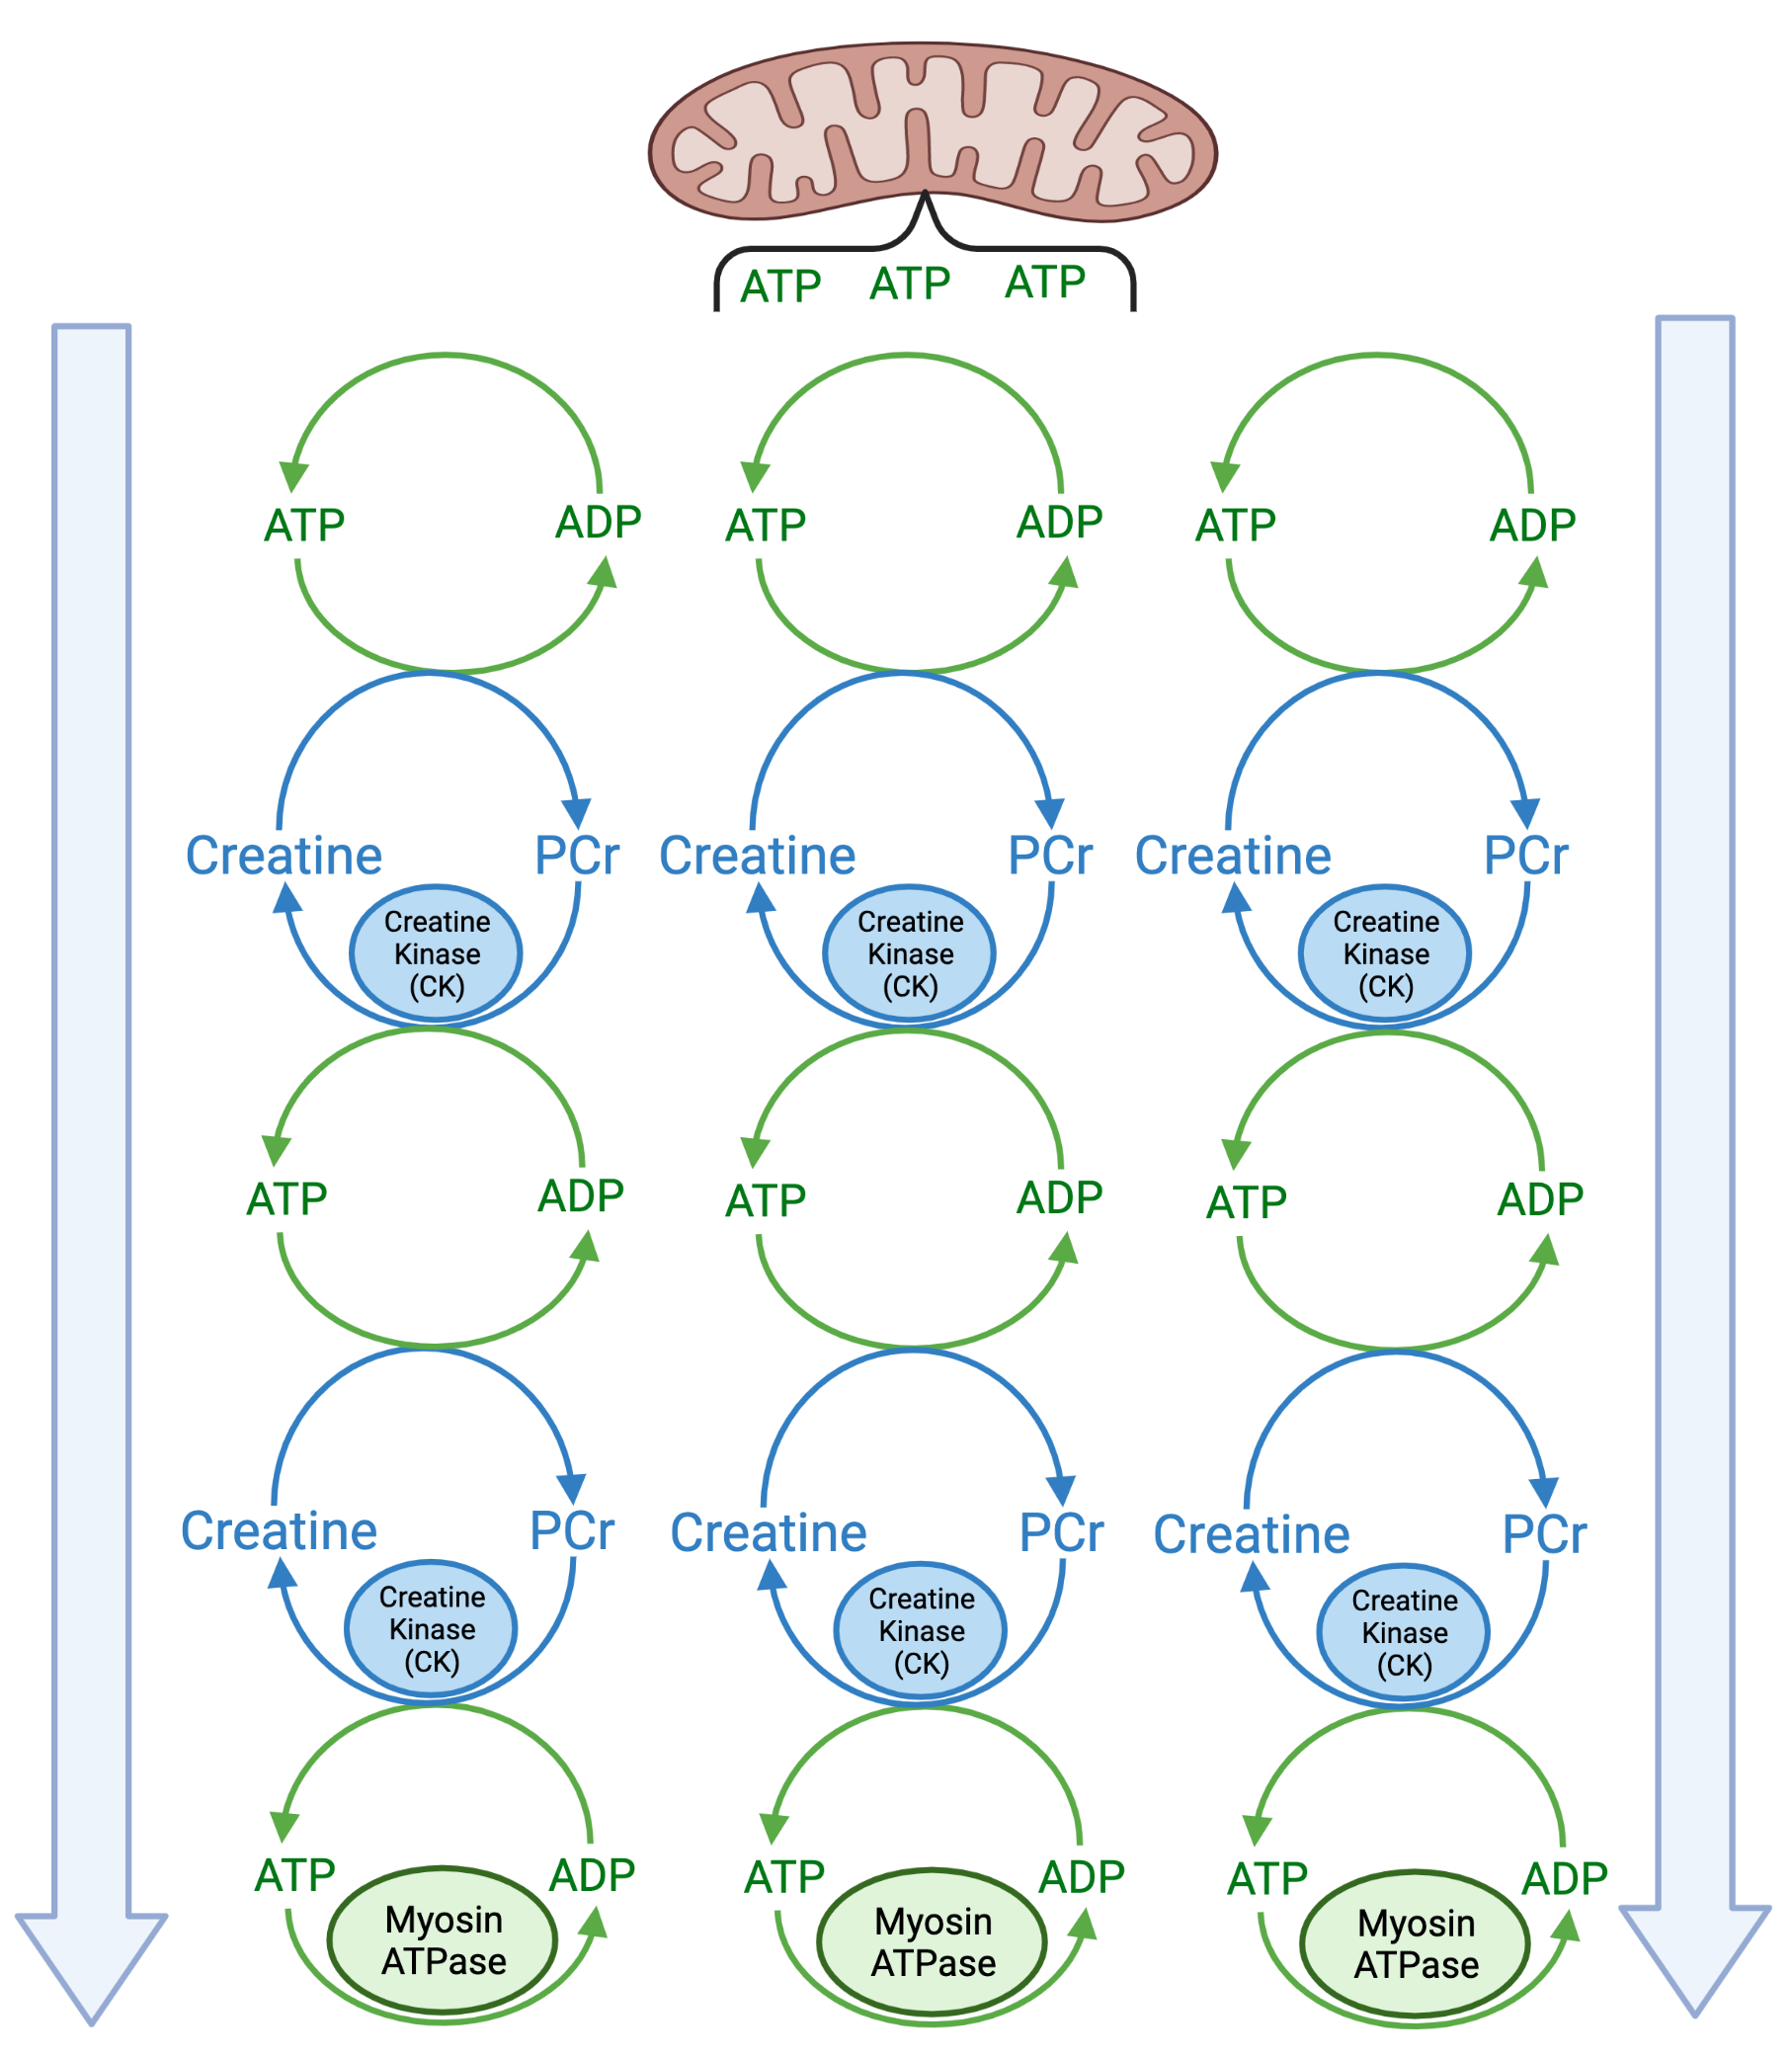
\includegraphics[width=0.75\linewidth]{./figure/PCr.png}
    \caption{Movement of ATP through the sarcoplasm using an ATP-PCr shuttle}
    \label{fig:PCr}
\end{figure}

\paragraph{Myokinase (Adenylate Cyclase)}

Another immediate high rate reaction to regenerate ATP is the myokinase enzyme (also referred to as adenylate cyclase) that catalyzes the reaction: $2ADP \rightleftharpoons AMP + ATP$. During this reaction a $P_i$ is hydrolyzed from ADP and the energy regenerates ATP. This reaction can happen at a high rate, but it is limited and probably only utilized in extreme ATP demand situations because in most situations ADP is being utilized by other pathways and not available for the myokinase reaction. But if there is a high enough accumulation of ADP myokinase allows continued cell functions for a short period of time. Estimates are that under conditions of maximum ATP utilization (upwards of 4.4 moles/minute), this system could be sustained for milliseconds (less than a second). It is self limiting because it is recycling a dwindling source of energy. For our purposes it is therefore added to the ATP/PCr row of Table \ref{table:ATP_Rates} given its relatively insignificant contribution to capacity. Though it may play a role in smoothing (buffering) responses to variable ATP demands.

\subsection{Muscle Glycogen $\rightarrow$ Lactate Pathway}

The muscle glycogen (or glucose) $\rightarrow$ lactate pathway provides ATP regeneration at a moderate rate. It is only capable of maximum rates for a relatively small amount of ATP and therefore for a short period of time. The key biochemical process for this pathway is glycolosis. 
Glycolosis transforms glucose or glycogen into several important end products including ADP to ATP, $NAD^+$ to $NADH$ and pyruvate. When regenerating ATP at high rates glycolosis ends up creating more $NADH$ and there is not enough $NAD^+$ to continue with glycolosis, and the accumulation of $NADH$ results in a drop in intracelluar pH. As a remedy to this situation $NADH$ is converted back into $NAD^+$ which includes the conversion of pyruvate into lactate.

The glycogen (or glucose) $\rightarrow$ lactate pathway, while always involved a bit, is primarily involved when it is functioning at a rate of ATP regeneration that exceeds the ability of the muscle glycogen $\rightarrow$ $CO^2$ pathway. A simplifying approach, based on the estimates in Table \ref{table:ATP_Rates}, is that if the glycogen (or glucose) $\rightarrow$ lactate pathway is generating over 1 mole / minute of ATP it is exceeding the rate that the muscle glycogen $\rightarrow$ $CO^2$ pathway. In this situation it is beneficial to the muscle fiber for lactate to form and be shuttled out of the cell to stabilize the pH and to make $NAD^+$ available to continue glycolosis. 

If the glycogen (or glucose) $\rightarrow$ lactate pathway towards lactate continues it eventually cannot shuttle lactate out of the cell fast enough and cellular pH drops (acidity), and there is not enough $NAD^+$, so the rate of glycolosis slows down (forcing a recovery period). A consequence for the muscle is that it cannot continue to generate tension at a rate that requires such a high rate of ATP regeneration.

\paragraph{Anaerobic Threshold - Lactate Threshold - Onset of Blood Lactate Accumulation}
Anaerobic threshold (AnT), lactate threshold (LT) and onset of blood lactate accumulation OBLA) are three related concepts. AnT is primarily theoretical and can be estimated by LT or OBLA which are both based on measurements of blood lactate. Ventilatory threshold (VT) is another approach to measuring AnT discussed in Chapter \ref{chp:fick_equation}. The concept of AnT is directly related to the previously discussed idea that when the glycogen (or glucose) $\rightarrow$ lactate is regenerating ATP at a rate higher than capable by the glycogen (or glucose) $\rightarrow$ $CO^2$ pathway, the pH of the cell drops and an increased amount of lactate is shuttled out of the cell into the blood. Active tension requiring ATP at a rate of regeneration that needs the glycogen (or glucose) $\rightarrow$ lactate pathway is not sustainable. The time that the active tension can be sustained is based on the different rates of the glycogen $\rightarrow$ lactate pathway and the glycogen$\rightarrow$ $CO_2$ pathway.

\subsection{Muscle Glycogen $\rightarrow$ $CO_2$ Pathway}

The muscle glycogen $\rightarrow$ $CO_2$ pathway provides ATP regeneration at less than half the rate as the muscle glycogen to lactate pathway. But it provides a sustainable source of ATP regeneration. It is not self limiting. There are factors and situations that emerge such as substrate (glycogen) availability that lead to fatigue and a need for recovery of this system. But as long as there is glycogen this pathway will continue to provide ATP regeneration to to its max rate. This pathway includes several biochemical processes. It begins with glycolosis which provides ATP, $NADH$ and pyruvate. The ATP is available for cellular energy. $NADH$ and pyruvate enter the mitochondria. Pyruvate is transformed into Acetyl-CoA which can enter the TCA cycle. The TCA cycle generates $CO_2$ for removal, ATP and more $NADH$. $NADH$ from glycolosis and TCA enter the ETC which transports electrons along the inner membrane of the mitochondria until they reach the final electron acceptor $O_2$. The transport of electrons pumps protons ($H^+$) between the mitochondrial membranes and develops a concentration and electrical gradient that pushes protons through ATP synthase (like water rushing through a dam). The ATP synthase rotates like a turbine and energizes the bond between ADP and $P_i$ to regenerate ATP. 

$CO_2$ is created as part of the citric acid cycle (TCA), $O_2$ is consumed as part of the electron transport chain (ETC). Note that $CO_2$ is produced and $O_2$ is consumed at different steps in the pathways that produce $CO_2$ as a byproduct and consume $O_2$. Together TCA and ETC are referred to as oxidative or aerobic metabolism. ETC is also oxidative phosphorylation. The availability of $O_2$ is critically important to the rate of ATP generated in all pathways using ETC. The use of $O_2$ in this pathway is the only use of $O_2$ in the human body. All $O_2$ consumed through respiration and measured through ventilatory tests such as indirect calorimetry are based on the use of $O_2$ in the mitochondria for the ETC. All estimates of metabolic rate that are based on $O_2$ consumption, including those using heart rate and steps taken, are founded in the fact that the ultimate source of most ATP (energy) passes through ETC and consumes $O_2$.

The muscle glycogen $\rightarrow$ $CO_2$ pathway produces the same volume of $CO_2$ as it consumes $O_2$. The ratio of $\frac{CO_2}{O_2}$ is referred to as the respiratory exchange ratio (RER). The RER for the muscle glycogen $\rightarrow$ $CO_2$ pathway is 1.0. However, it is not the only pathway that results in an RER = 1.0. 


\subsection{Liver Glycogen $\rightarrow$ $CO_2$ Pathway}

The liver glycogen $\rightarrow$ $CO_2$ pathway is similar to the muscle glycogen $\rightarrow$ $CO_2$ pathway. One difference is that the rate of ATP production is lower due to the need to breakdown glycogen in the liver and circulate it through the blood to the extracellular fluid of the muscle for transport into the muscle. There is also a lower overall capacity because more glycogen is stored in muscles (in total) than in the liver. Breakdown of liver glycogen into blood glucose can be used by muscles to either immediately enter glycolosis. If not needed for glycolosis this glucose can be stored as glycogen. Once glucose enters glycolosis it basically follows the same path as the muscle glycogen $\rightarrow$ $CO_2$ pathway. Whether starting with liver glycogen or with muscle glycogen these two pathways produce the same volume of $CO_2$ as they consume $O_2$, at they both of an RER = 1.0. These are the only two pathways with an RER = 1.0. Therefore, at rest an RER of 1.0 would indicate that a glucose or glycogen pathway to $CO_2$ was the dominant energetic pathway. Variations to this during activity are discussed in Chapter \ref{chp:fick_equation} on the Fick Equation.

\subsection{Fatty Acids $\rightarrow$ $CO_2$ Pathway}

The fatty acid $\rightarrow$ $CO_2$ pathway has the lowest overall rate of ATP regeneration.\footnotemark\footnotetext{Note that this finding is based on years of experiments in individuals consuming typical carbohydrate dominant diets. Research in subjects that are fat adapted challenge this paradigm, suggesting that it is possible, with fat (keto)adaptation that the fatty acid $\rightarrow$ $CO_2$ pathway may not have as significant a drop in the rate of ATP utilization as previously believed \cite{mcswiney_keto-adaptation_2018}.} The substrate for this pathway are fatty acids carried in the blood as ketones. The process of generating ketones is covered in Chapter \ref{chp:blood_nutrients}. Despite the lower rate there is a huge capacity for continued ATP regeneration with fatty acids due to the generally larger storage of fat in adipose tissue in even lean individuals, and the higher energy density of fat (approximately twice the energy yield per gram than glucose or glycogen). Fatty acids enter the muscle fiber and the mitochondria and are converted to several acetyl-CoA molecules (exact number depends on the number of carbons in the fatty acid). Acetyl-CoA is the first step to TCA which produces $CO_2$ for removal and $NADH$ for ETC. Once a fatty acid is converted to acetyl-CoA the pathway is identical to the pathways starting with liver or muscle glycogen. The higher energy (ATP) yield when using fatty acids is related to the number of acetyl-CoA molecules formed when using the same number of grams of fat as compared to glucose or glycogen. 

The RER when fatty acids are utilized tend to be less than 0.75 (the exact RER varies depending on the fatty acid utilized). A mixed diet at rest typically results in an RER $\approx$ 0.85. A predominantly glucose (carbohydrate) diet will increase the RER toward 1.0. A fat based (keto) diet lowers the RER \cite{alessandro_effects_2015}.

\subsubsection{Pathways for Protein Energetics}

There are a variety of pathways for protein energetics, but they are not an optimal source of energy and not the best use of protein. The pathways are reserved for extreme situations. These pathways involve protein breakdown into amino acids and the use of amino acids at various steps of other pathways (requires removal of nitrogen). The two primary paths for protein involve the use of amino acids to produce acyetyl-CoA, and in the liver for gluconeogenesis. Gluconeogenesis is the generation of glucose from non carbohydrate carbon sources including amino acids (as well as other molecules such as lactate, pyruvate, acetyl-CoA and fatty acids).

\subsection{Rates and Capacities}

Rates and capacities of ATP regeneration for each of the pathways are included in Table \ref{table:ATP_Rates}.

\begin{table}[h!]
\centering
\begin{tabular}{||c c c c||} 
 \hline
Source & Max Rate of ATP (mol/min) & Amount of ATP (mol) & Time at Max (s or min)\\ [0.5ex] 
 \hline\hline
 ATP/PCr/Myokinase & 4.4  & 0.7 & 10 s \\
 Muscle Glycogen $\rightarrow$ Lactate &  2.4 & 1.6 & 40 s \\ 
 Muscle Glycogen $\rightarrow$ $CO_2$ & 1.0 & 84 & 84 min\\
 Liver Glycogen $\rightarrow$ $CO_2$  & 0.5 & 30 & 60 min \\ 
 Fatty Acids $\rightarrow$ $CO_2$ & 0.4 & 4000 & 10,000 min \\[1ex] 
 \hline
\end{tabular}
\caption{Summary of Max Rates of ATP Regeneration by Pathway (\footnotesize{Data from \cite{feher_quantitative_2017}})}
\label{table:ATP_Rates}
\end{table}

When considering the time estimates based on the quantity of ATP can be be regenerated by various energetic pathways it is important to consider that two factors influence the sustainability of the pathway. First whether the pathway, at or near its max rate, is rate limiting. Second, the availability of the substrate (macro-nutrients) in storage. The time estimates in Table \ref{table:ATP_Rates} are calculated based on the assumption of the max rate. For example, the 10 second estimate for ATP/PCr is based on the max rate of ATP regeneration from ATP/PCr. If the demand for ATP by the muscle is 2.2 mol/min then the time that ATP/PCr could contribute would be approximately 19 seconds. If the demand for ATP by the muscle is 1.1 mol/min then the time that ATP/PCr could contribute would be approximately 38 seconds. By this time the muscle glycogen $\rightarrow$ lactate pathway could be contributing and meeting most of the ATP demand of the muscle. 


Table \ref{table:Event_ATP_Rates} provides estimated rates of ATP consumption and the amount of ATP utilized for a variety of timed running events. Comparing this data to Table \ref{table:ATP_Rates} allows the reader to consider which energetic pathways are capable of regenerating ATP at rates high enough for the various events.


\begin{table}[h!]
\centering
\begin{tabular}{||c c c c||} 
 \hline
Events & Rate of ATP Consumption (mol/min) & Amount of ATP (mol) & Estimated Time (s or min)\\ [0.5ex] 
 \hline\hline
 Rest & 0.12  & 173 & One Day \\
 100 Meter Sprint & 2.8 & 0.5 & 10 seconds \\ 
 800 Meter Run & 2.0 & 3.4 & 192 seconds\\
 1500 Meter Run & 1.7 & 6 & 210 seconds \\ 
 42,0000 Meter Run & 1.0 & 150 & 150 minutes \\[1ex] 
 \hline
\end{tabular}
\caption{Estimated Rate of ATP Consumption during Various Timed Running Events (\footnotesize{Data from \cite{feher_quantitative_2017}. Resting data is estimated based on basal energy expenditure of 1200 calories, and a conversion rate of about 6.93 calories per mole of ATP.})}
\label{table:Event_ATP_Rates}
\end{table}
 
A 100 meter sprint requires a mix of ATP/PCr and muscle glycogen $\rightarrow$ lactate pathway. The 800 meter and 1500 meter runs require a mix of ATP/PCr, muscle glycogen $\rightarrow$ lactate and muscle glycogen $\rightarrow$ $CO_2$ pathways. The 42,000 meter run will rely on the slower rate but higher capacity pathways of muscle glycogen $\rightarrow$ $CO_2$, liver glycogen $\rightarrow$ $CO_2$ and may require some fatty acid to $CO_2$ depending on the exact quantity of ATP capable of being generated by muscle and liver glycogen. There is debate about the ability of fat adaptation to improve the performance of endurance athletes. No one questions whether there is a higher overall capacity (storage) when using fat as the substrate of choice, such as with fat adaptation and a low carbohydrate diet. The question is whether the fatty acid $\rightarrow$ $CO_2$ pathway is capable of providing the same, or at least close enough, rate of ATP regeneration as the muscle and liver glycogen pathways \cite{mcswiney_keto-adaptation_2018}.

\section{Motor Unit \& Muscle Fiber Types}

Chapter \ref{chp:regulation} discussed the fast and slow twitch characteristics of motor units and muscle fibers based on the concepts of excitation and activation. There are also energetic differences between motor unit muscle fiber types. These characteristics can be inferred by the labels "O" for oxidative and "G" for glycolytic. The energetic differences between the three classifications of muscle fibers are provided in Table \ref{table:Muscle_Fiber_Energetics}. Four energetic characteristics are compared based on high (+++), medium (++) or low (+) relative capacities of the fiber types. 

\begin{table}[h!]
\centering
\begin{tabular}{||c c c c c||} 
 \hline
 Muscle Fiber Type & Mitochondria & Myoglobin & Glycolytic Enzymes & PCr \\ [0.5ex] 
 \hline\hline
 Fast Glycolytic (FG)  & + & + & +++ & +++ \\ 
 Fast Oxidative Glycolytic (FOG) & ++ & ++ & ++ & ++ \\
 Slow Oxidative (SO) &  +++ & +++ & + & + \\ [1ex] 
 \hline
\end{tabular}
\caption{Energetic Characteristics of Muscle Fiber Types}
\label{table:Muscle_Fiber_Energetics}
\end{table}

\paragraph{Slow Oxidative (S/SO/Type 1}

SO fibers have a greater number of mitochondria and more myoglobin than FG and FOG fibers. These fibers are better equipped to sustain ATP production. It would be expected that muscles with more SO fibers would have higher rates of ATP production utilizing the energetic pathways that rely on TCA and ETC. This supports the ability to provide tension for a longer period of time.

\paragraph{Fast Glycolytic (FF/FG/Type 2a}

FG fibers have a greater number of glycolytic enzymes and more PCr available which maximizes the anaerobic (high rate of ATP production outside of the mitochondria) pathways. They are higher rates of ATP production for the PCr and muscle glycogen to lactate pathways, which result in higher rates of ATP production overall. However, these high rates of ATP regeneration are not sustainable. This supports the higher tension capability of these fibers. Based on the ATP-PCr shuttle (Figure \ref{fig:PCr}) the elevated PCr throughout FG muscle fibers can quickly propagate ATP regeneration through the muscle fiber to the areas most needed, and the regeneration of PCr from ATP released from the mitochondria during recovery.

\paragraph{Fast Oxidative Glycolytic (FR/FOG/Type 2x}

FOG fibers have a moderate number of all energetic characteristics. They can attain more tension than the SO fibers but cannot sustain it as long as SO fibers. They can sustain tension longer than FG fibers, but cannot attain as high a tension as FG fibers. 

\section{\textit{Clinical Physiology Connections}}

\subsection{Sarcopenia}

Sarcopenia is an age related loss of muscle fibers with a bias toward FG fibers (FF motor units). A consequence of sarcopenia is a loss of the ability to attain the upper ranges of muscle tension. Expected consequences are a reduction in peak tension, high forces and high velocities of movement. An unexpected, paradoxical, consequence is a reduction in the ability to sustain lower ranges of muscle tension such as those required during activities of living such as walking. This paradoxical consequence is based on the need to recruit the remaining motor units with increased frequency to meet the tension requirements of movement. Recruiting a slow motor unit and its SO fibers more frequently (higher frequency summation) requires a higher rate of ATP than can be sustained. There is no question that S motor units and SO muscle fibers can achieve a higher rate of ATP regeneration than FF motor units and FG muscle fibers. But at a high level of tension (relative to the motor units capacity) the higher rate of crossbridge activation requires a higher rate of ATP regeneration. If that higher rate of ATP regeneration is greater than the rate capacity of the glycogen $\rightarrow$ $CO_2$ pathway, then the fiber will need to utilize the glycogen $\rightarrow$ lactate pathway, which is self limiting (cannot be sustained). 

Let's walk through this with a simple model example. Assume walking requires 50\% output (tension) of 1/4 of the motor units. At this output the fibers require 0.7 moles of ATP / minute. In this scenario the Glycolosis $\rightarrow$ $CO_2$ pathway is sufficient and the activity is sustainable. Now assume there has been a loss of motor units. Now there are 1/2 of the prior motor units, and they are predominantly lower tension generating (S/SO) because the loss (due to sarcopenia) results in a loss of FG/FOG muscle fibers. Now walking (at the same pace as before) requires 75\% output from 3/4 of the fibers (since a twitch generates less tension there needs to be more frequency and motor unit summation). At this output the fibers require 1.3 moles of ATP / minute. In this scenario the Glycolosis $\rightarrow$ $CO_2$ pathway is not sufficient and the Glycolosis $\rightarrow$ Lactate pathway must be utilized to supplement ATP regeneration, which is not sustainable. Continuing to walk at this pace will result in fatigue. That is the paradoxical consequence of the loss of FF motor units in sarcopenia. Everyone expects a loss in the ability to attain tension as measured by peak force. But there is also a loss in the ability to sustain tension as measured by the ability to continue developing tension for an activity.


\subsection{Fatigue}

% Robustness (surge capability) - sensing the reserve
% Fidelity - objective (outward) 
% Efficacy - subjective (inward - how am I doing this act, how is it being supported?)
% Integrity - you need the reserve, so don't completely exhaust it / use it
% Fatigue - roll up, signal, regarding sustaining (and then can't attain what you started with)

Biological systems include cycles. Ca+ is released and taken in, muscle fibers develop active tension and then they don't, movements happen then they don't, we are awake and then asleep. Across all scales in biological systems there are cycles. These cycles include using resources, capabilities, and reserves and then building them back up. The concept of fatigue is fundamentally about these cycles. At the most general level fatigue occurs when resources, capabilities and reserves have been utilized and it is time for the cycle to be completed and go to its recovery phase. If the cycle that leads to fatigue is not completed so that recovery can begin, then fatigue occurs.

Fatigue is a widely utilized concept because it can be applied to any aspect of a system with cycles occurring at any scale, which is any system doing an act, which is any system. Reading about fatigue is sure to result in several different interpretations. Muscle fatigue is the inability continue to sustain a tension with repeated excitation, and with fatigue the inability to attain a previously attainable tension. Running fatigue is the inability to sustain a pace with continued running, and the inability to attain that pace until recovery has occurred. Mental fatigue influences the ability to concentrate. Cognitive fatigue influences the ability to do complex tasks. Physical fatigue can reduce the maximal heart rate that can be achieved with exertion, or a higher heart rate at a given sub maximal workload. Chronic fatigue syndrome is characterized by a severe lack of energy following exertions. The descriptions of fatigue can be like the description of the elephant by blind monks in Figure \ref{fig:elephant}. One monk describes the elephant as like a rope (while feeling the tail), another like a snake (while feeling the trunk), another like a wall (while feeling the body), another like a tree trunk (while feeling a leg), another like a spear (while feeling the tusk), and another like a large sheet (while feeling the ear).    

\begin{figure}[!h]
    \centering
    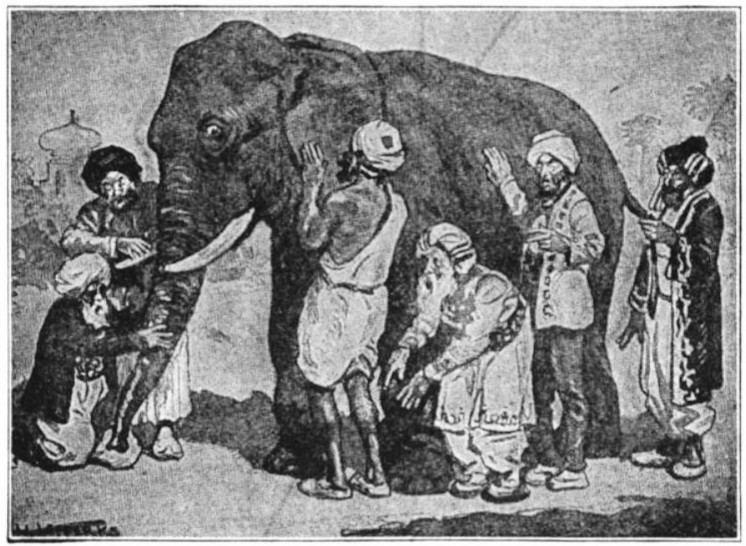
\includegraphics[width=1\linewidth]{./figure/elephant.jpg}
    \caption{Five Blind Monks Describing an Elephant (\footnotesize{Public Domain from \href{https://commons.wikimedia.org/wiki/File:Blind_men_and_elephant.png}{Sophie Woods, World Stories for Children, Ainsworth & Co. (Chicago), p. 14}})}
    \label{fig:elephant}
\end{figure}

A general definition of fatigue is an inability of a system (In our case a biological system) to accomplish its act. Fatigue is therefore a failure to achieve act objectives. Note that this meaning is objective. The fact that the act cannot achieve its objective is measurable in some way. This is an objective definition of fatigue that can be applied in many contexts.

There is also a subjective perspective of fatigue. The subjective perspective, at least in terms of human fatigue, is the feeling (perception) of fatigue. Sometimes people confuse the subject and the objective. Notice again that the objective perspective of fatigue includes the inability of the system to achieve its act based on some measurable objective. If the system is meeting the objective of its act then it is not fatigued. However, there may be a perception of fatigue, and the person can report that they are fatigued. Both need to be considered and both pieces of information are important. For example, if a person walking 4 mph on a treadmill starts to feel fatigued during this act but they can accomplish the act then they are not objectively fatigued (they are doing the act), but they are subjectively feeling fatigued (or perhaps tired; or out of breath which can be confused symptomatically with fatigue). The new symptom of (perception of) fatigue in this individual despite being able to meet the objective of the act means that the person is not fatigued for the act of walking at the point they are doing the walking. But that perception is probably arising because the reserve capacity for the act is being utilized to some level that is signaling its nearly time to enter a recovery phase. It could be some supporting system for that act of walking is fatigued and perhaps in an objective measurable (but not currently measured) act. That failure results in the need for other support systems to provide more support than usual to the walking act. Whether the fatigue in these support system can compensate or not, whether they are sustainable or not, influences whether, and if so how long, the walking act at 4 mph can continue. Once all possible support systems are fatigued then the walking act will no longer be able to continue at 4 mph, so the person slows down the treadmill to 3 mph and they are doing a new act that they can continue. At this new walking act, the energetic requirements may be low enough that all of the support systems recover to full capability and the person can go back to 4 mph for a time being. The change in the ability - previously being able to do 4 mph without fatigue to now not being able to do 4 mph without fatigue - can be due to a large number of factors. Relevant to this chapter it may be due to the amount of substrate available, or state of the muscle fibers (perhaps there has been a loss of mitochondria due to reduced use of the muscles), or perhaps deficiency in creatine that is slowing down transport of ATP through the sarcoplasm so that the muscle glycogen $\rightarrow$ $CO_2$ pathway ATP needs to be supplemented with the muscle glycogen $\rightarrow$ lactate pathway.

Based on the above example it is hopefully clear that the applications of the concept of fatigue vary based on time and space scales, and that these scales are superimposed. As we consider longer time scales all of the acts that can occur within that time scale are important. As we consider higher spatial scales, all of the acts at spatial scales below it are important. If the act is walking for 4 hours at a 4 mph pace then all of the acts within 4 hours, at all of the scales (walking requires tension in a particular set of muscles, each muscle must generate the right tension, each motor unit contributes the tension it must contribute, each muscle fiber contributes its share of the tension which requires the fiber to be utilizing and regenerating ATP). Walking today for 4 hours at 4 mph may be achieved (no fatigue for walking at 4 mph for 4 hours) with the perception of fatigue (subjective, so most likely some acts in supportive roles were fatigued). The next day the act of walking for 4 hours at 4 mph may not be achieved - there may be objective fatigue the next day. An act today with no fatigue, but performed everyday may result in fatigue in upcoming days. The point is that system must have time to recover from fatigue. 

Table \ref{table:fatigue_recovery} provides experimentally derived estimates of fatigue recovery times for a variety of physiological components important for considering low back injury. These times were used to build a model of low back fatigue and recovery as a dynamic predictor of low back injury at work based on the work recovery exposure cycles. The basic idea is that it is not just the work demands, but the time to recovery between demands, that influences injury risk.

\begin{table}[h!]
\centering
\begin{tabular}{||c c ||} 
 \hline
 Fatigued System & Recovery Time\\ [0.5ex] 
 \hline\hline
 Myoglobin stores & 10-15 seconds to 1 minute \\
 Conduction Velocity  & 5 minutes\\ 
 PCr & 10 minutes  \\
 ATP stores &  Minutes (2-5) \\ 
 Lumbar flexion creep & 30+ minutes \\
 Lactate removal & 25 minute half life \\
 Intramuscular pH & 20-30 minutes \\
 EMG Amplitudes & 30 minutes \\
 Body Height after lumbar disc compression & 4 hours \\
 Ligament laxity & 7 hours \\
 Muscle glycogen & 5-24 hours \\[1ex] 
 \hline
\end{tabular}
\caption{Experimentally Derived Estimates of Recovery from Fatigue in Various Systems. Readers should not attempt to memorize the actual times. This data is presented to emphasize the point about fatigue from different systems across scales and times for recovery. Data is from \cite{krajcarski_time_2008}.}
\label{table:fatigue_recovery}
\end{table}

\paragraph{}
The perspective of objective and subjective fatigue does not intend to diminish the importance of subjective fatigue experiences. Just to keep both perspectives in mind. These perspectives give rise to the perspectives of absolute and relative workload. Walking at 4 mph is an absolute workload. If that workload can be achieved without objective fatigue at the level of the required act for 4 hours then that absolute workload is 4 mph for 4 hours. The subjective fatigue is the relative workload, how hard did the person need to work (or push, or strain) to complete that absolute workload? Relative workload can be measured with a rating of perceived exertion (technically different but relatable to subjective fatigue), or by measures of other systems that support the absolute workload of walking such as heart rate, blood flow, ventilation rate, blood lactate, oxygen consumption, carbon dioxide production. 

\subsubsection{Energetic Fatigue}

Table \ref{table:ATP_Rates} provides estimates of ATP regeneration rates based on the energetic pathways. Each energetic pathway leads to muscle fatigue when its capacity (Amount of ATP) has been utilized. When its capacity has been utilized it must, as a pathway, recover. The time it takes for a pathway to utilize its capacity is dependent on the rate of ATP regeneration required by the muscle fibers need for ATP. When you are preserving battery life on your phone you shut down apps in the background to minimize the rate of energy depletion and extend batter life. Subjective fatigue (the perception of fatigue) is often felt prior to complete depletion. Most likely as a warning sign to consider "shutting down some apps" prior to the point when the act can no longer be performed due to objective fatigue. 

The recovery of each system is specific to the system. For the PCr pathway, ATP is needed to regenerate PCr and can take several minutes (Table \ref{table:fatigue_recovery}). For the muscle glycogen $\rightarrow$ lactate pathway recovery would include a fresh supply of $NAD^+$ from ETC and the reduction in lactate. For muscle and liver glycogen $\rightarrow$ $CO_2$ pathways recovery would be new stores of glycogen (hours to days). Fatty acid $\rightarrow$ $CO_2$ pathway is one of those systems that tends to function with little need for recovery for a really long time. Efforts to preserve fatty acids (a form of recovery through slower utilization) could include breaking down protein and generating glucose with gluconeogenesis in the liver. But even during sustain activity other systems, or other aspects of muscle function, are most likely going to fatigue before fatty acid energetics fatigue (such as the brain requiring sleep; or muscle tissue breakdown, or connective tissue breakdown both due to prolonged overuse, for example). Since walking is a pace that people can sustain with the fatty acid $\rightarrow$ $CO_2$ pathway it is unlikely that the fatigue during a 20 mile walk is due to energetics. However, that does not mean that a person untrained for such a walk would not have blisters, dehydration, chaffing and several other problems due to various systems being fatigued.

How an activity influences muscle fatigue is based on the overload. The overload training concept is the stimulus for training related muscle adaptations. Training adaptations often occur in response to training fatigue in an attempt to build system capacity to avoid future fatigue. The relationship between fatigue and training adaptations is provided in Chapter \ref{chp:myostasis} on Myostasis.

\subsection{Hypoxia, Hypoxemia \& Ischemia}

The oxidative energetic pathways provide most of the ATP for cellular functions and are critically involved in the restoration of the energetic resting state following short term rate increases in ATP production with PCr, myokinase or glycolosis. The oxidative (mitochondrial) pathways require oxygen and macro-nutrient substrate (seconds-minutes). Over longer time periods (hours-days) they require cellular synthesis of enzymes which require ATP and amino-acids (to build proteins). And over longer time periods (days-weeks) they require maintenance of the health of mitochondria and replacing damaged or dead mitochondria. Interruptions in the availability of $O_2$ interrupts the process of ATP production with these pathways and can lead to the accumulation of metabolic waste products that alter the pH of the cell and the extra-cellular fluid. These interruptions form the basis of a large number of relatively common and life-threatening chronic medical conditions such as heart disease, stroke, peripheral vascular disease, COVID-19, pulmonary disease, and hematologic (blood) conditions; as well as sudden onset (acute) conditions such as a heart attack and acute altitude sickness. 
Some of the conditions have a rapid onset and immediately threaten life; others exert their effect gradually. The variation is related to rate of onset of $O_2$ deprivation, the magnitude of $O_2$ deprivation (how much deficit, how many cells), and whether the impact is just in the availability of $O_2$ or whether there is also an impairment in waste product removal. But they can all be analyzed based on an understanding of cellular energetics and the role that ATP plays in cellular fidelity, efficacy and integrity.

\paragraph{Hypoxia}
Hypoxia refers to the situation in which there is not enough $O_2$ getting to cells for them to sustain the oxidative production of ATP. It is a form of fatigue since the resources of ETC are not available it cannot achieve act objectives (ETC cannot generate enough ATP because there isn't enough $O_2$). Hypoxia can be caused by a variety of situations. It is a local condition because it depends on local $O_2$ levels and local $O_2$ needs. Local $O_2$ needs are dependent on the local need for ATP (metabolism). Cells of the body that have relatively high and constant $O_2$ needs, and are therefore more susceptible to hypoxia, are the heart and brain. Metabolism is always related to cellular activity and the cells of these two organs generally have a higher resting metabolism than other cells. Muscle metabolism can far exceed that of both heart and brain, that is only during periods of high muscle activity which require high levels of ATP production. 
Common causes of hypoxia are hypoxemia and ischemia.

\paragraph{Hypoxemia}
Hypoxemia is a specific situation in which the blood isn't carrying adequate oxygen to body tissues. Common causes of hypoxemia include pulmonary and blood conditions (for example, obstructive pulmonary disease and anemia) or environmental conditions (altitude, carbon monoxide). 

Hypoxemia can cause hypoxia. The severity of hypoxia in a cell caused by hypoxemia is dependent on the severity of hypoxemia as well as the energetic activity of the cell (ATP regeneration rate which determines $O_2$ demand), which fluctuates based on several factors. In someone with mild hypoxemia there may be no hypoxia in cardiac or skeletal muscles. However, with exertion that increases cardiac and skeletal muscle activity and thus need for $O_2$ ($O_2$ demand) there may be hypoxia. In these situations cardiac and skeletal muscle function will be impaired by the lack of $O_2$. The cellular adjustment will be to provide ATP using a higher rate of anaerobic pathways which is not sustainable. The by-products of these activities decrease the cellular and extra-cellular pH which further impair ATP regeneration. The acidosis and reduced ATP relative to need can impact the ability of the cells to repolarize, reduce the frequency of excitations, reduce the pumping of Ca+ back into the sarcoplasmic reticulum, reduce the rate of myosin head release. The consequences of these changes include lower tension production, spasm and potentially damage to the cell membrane. But typically, if the problem originates with hypoxemia that is adequate for resting levels of $O_2$ demand then simply ceasing the activity will restore balance and not result in damage to the cell membrane.
 
\paragraph{Ischemia}
Ischemia is a specific situation in which  blood supply to cells is reduced. The extent of cellular involvement depends on the extent of the reduction. For example, if an entire artery is impacted than an entire limb, or muscle can be involved. If the reduction occurs in capillaries then the reduction in blood flow is to far fewer cells. Common causes of ischemia are atherosclerosis, arteriosclerosis,\footnotemark\footnotetext{Arteriosclerosis refers to thick and stiff arteries that can restrict blood flow. Atherosclerosis is a type of arteriosclerosis that includes buildup of fats, cholesterol and other substances in and on artery walls (plaque). The subsequent reduction in vessel diameter limits blood flow, and if a plaque becomes an embolus it can lodge and completely block blood flow (blood clot).} blood clots (arterial thrombosis or embolus, or in the case of pulmonary blood flow venous thrombosis or embolus), blood vessel spasm, and micro-circulatory inflammation (a clinical manifestation of hypoxia itself and seen in COVID-19). 

Ischemia can cause hypoxia. The severity of hypoxia in a cell caused by ischemia is dependent on the severity of ischemia as well as the metabolic activity of the cell ($O_2$ demand). A sudden and complete blockage of blood flow to cells, with no alternative pathways to provide blood flow to the cell, is a serious situation that results in cellular death due to the inability to produce ATP for cell membrane functions (sudden complete hypoxia) and to remove waste products. The combination of these two situations results first in reversible damage to the cell membrane and then to irreverisble damage to the cell membrane. Without the cell membrane the cell has lost its integrity. Less extreme reductions in blood flow can create a wide variety of hypoxic and waste removal situations that allow sustained but reduced function for a cell (resulting in long term problems in cell maintenance), and reduced function of the cells. For example, a limit on how much activity the cardiac or skeletal muscle can perform prior to having hypoxia. It is common to simply refer to such situations as ischemia (which means local blood flow is reduced and $O_2$ demands are high enough to cause hypoxia. 

Given the variable nature of blood flow supply and cellular $O_2$ demand there are two situations that can arise for cardiac muscle cells in particular. Stable ischemia refers to the situation that blood flow is sufficient for resting $O_2$ demand, but not sufficient during elevated $O_2$ demand (increased cardiac muscle activity). The situation is considered stable because simply reducing cardiac activity will reduce cardiac $O_2$ demand and restore balance to allow recovery. Unstable ischemia refers to the situation that blood flow is not sufficient for resting $O_2$ demand. Unstable ischemia is unstable because balance cannot be restored by reducing the cardiac muscle activity back to rest since it is the resting demand that cannot be met. In such situations blood flow must be restored, or cardiac muscle $O_2$ demand must be reduced below resting levels. Restoring blood flow is highly situational and can involve breaking up a blood clot (thrombus) with medications (thrombolytic therapy); or restoring the diameter of blood vessels with an angioplasty or by re routing the blood (by-pass graft. Reducing cardiac muscle $O_2$ demand can be accomplished by lowering blood pressure (blood pressure is the resistance that the cardiac muscle must work). Nitroglycerine is a very powerful and fast dilator of blood vessels that quickly lowers blood pressure and allows the cardiac $O_2$ demand to be lowered below resting values. The hope is this restores balance between $O_2$ supply and $O_2$ demand and the cells to recover before damage.

A consequence of ischemia that is not present in hypoxemia is the removal of waste products. Since blood flow to a region of the body does two things for the local extra cellular fluid - deliver $O_2$ and nutrients and remove waste - ischemia results in a loss of both. Therefore, the reduction in pH associated with prolonged anaerobic energetic pathways without sufficient aerobic pathway contribution is worse with ischemia than with hypoxemia. With hypoxemia the lactate in the surrounding extra-cellular fluid is removed. But with ischemia removal is impaired. 

\paragraph{Hypoxia Summary}
Hypoxia is the basis of the homeostatic imbalances caused by many conditions and diseases. It is based on the cellular requirements for ATP, which are based on the mitochondrial requirements for $O_2$. Cells can produce ATP without $O_2$, however they cannot sustain the production of ATP without $O_2$. Understanding these mechanisms and that of hypoxia offers a wellspring of conceptual insights for many diseases and pathophysiological conditions that go well beyond the above discussion. Hypoxia caused by hypoxemia or ischemia continues to be topic for several of the upcoming chapters on Muscle Support.

\section{Chapter Summary}

ATP is critical to muscle fibers and all cells. Muscle fibers have limited ATP reserves and can experience a 60 to 100 fold increase in the utilization and therefore need to regenerate ATP. There are several energetic pathways for the regeneration of ATP that are all always functioning.  Each pathway contributes different max rates of ATP production and different capacities. The max rate of ATP regeneration and the overall capacity of ATP regeneration of the energetic systems are inversely proportional. The pathways can be generally classified as anaerobic (occurring outside the mitochondria and not using $O_2$ or producing $CO_2$) and aerobic (occurring inside the mitochondria and using $O_2$ and producing $CO_2$). The anaerobic pathways have higher rates of ATP regeneration and lower capacities, whereas the aerobic pathways have lower rates of ATP regeneration and higher capacities. The three muscle fiber types are each uniquely adapted to three different combinations of energetic characteristics. These adaptations are well matched to the tension generating capabilities of these fibers as discussed in Chapter \ref{chp:regulation}. 

Sarcopenia results in the loss of predominantly FG muscle fibers. Combining the recruitment required to meet tension needs it becomes possible to explain the paradoxical reduction in endurance in people with sarcopenia. 

Fatigue is objectively the inability of a system to accomplish its act. Fatigue is therefore a failure to achieve act objectives. Fatigue occurs when a system resources, capabilities or reserves are used up and must be recovered. This pattern of using up and then restoring resources, capabilities or reserves is cyclic. The cycles of fatigue and recovery occur at all levels of biological systems, and across several time scales. Subjective fatigue refers to the perception of fatigue (feeling fatigue in some way). Subject fatigue is based on the sensations that arise when system resources, capabilities or reserves are being depleted whether or not there is objective fatigue. Energetic fatigue of muscles is based on the ability of the energetic pathways to continue to regenerate ATP.

Hypoxia occurs when there is not enough $O_2$ for ETC to function normally and therefore provide enough ATP. It is based on $O_2$ availability and how much ATP is needed by the cell. It is a form of fatigue since the resources of ETC are not available it cannot achieve act objectives (ETC cannot generate enough ATP because there isn't enough $O_2$). Hypoxemia is a reduction in $O_2$ in the blood and therefore can cause hypoxia. Ischemia is a reduction of blood flow to cells and therefore can cause hypoxia. Ischemia additionally disrupts the removal of cellular waste products and therefore the maintenance of the local extra-cellular fluid surrounding the ischemic cell. 

\section{Part I Summary \& Next Steps}

\begin{figure}[!h]
    \centering
    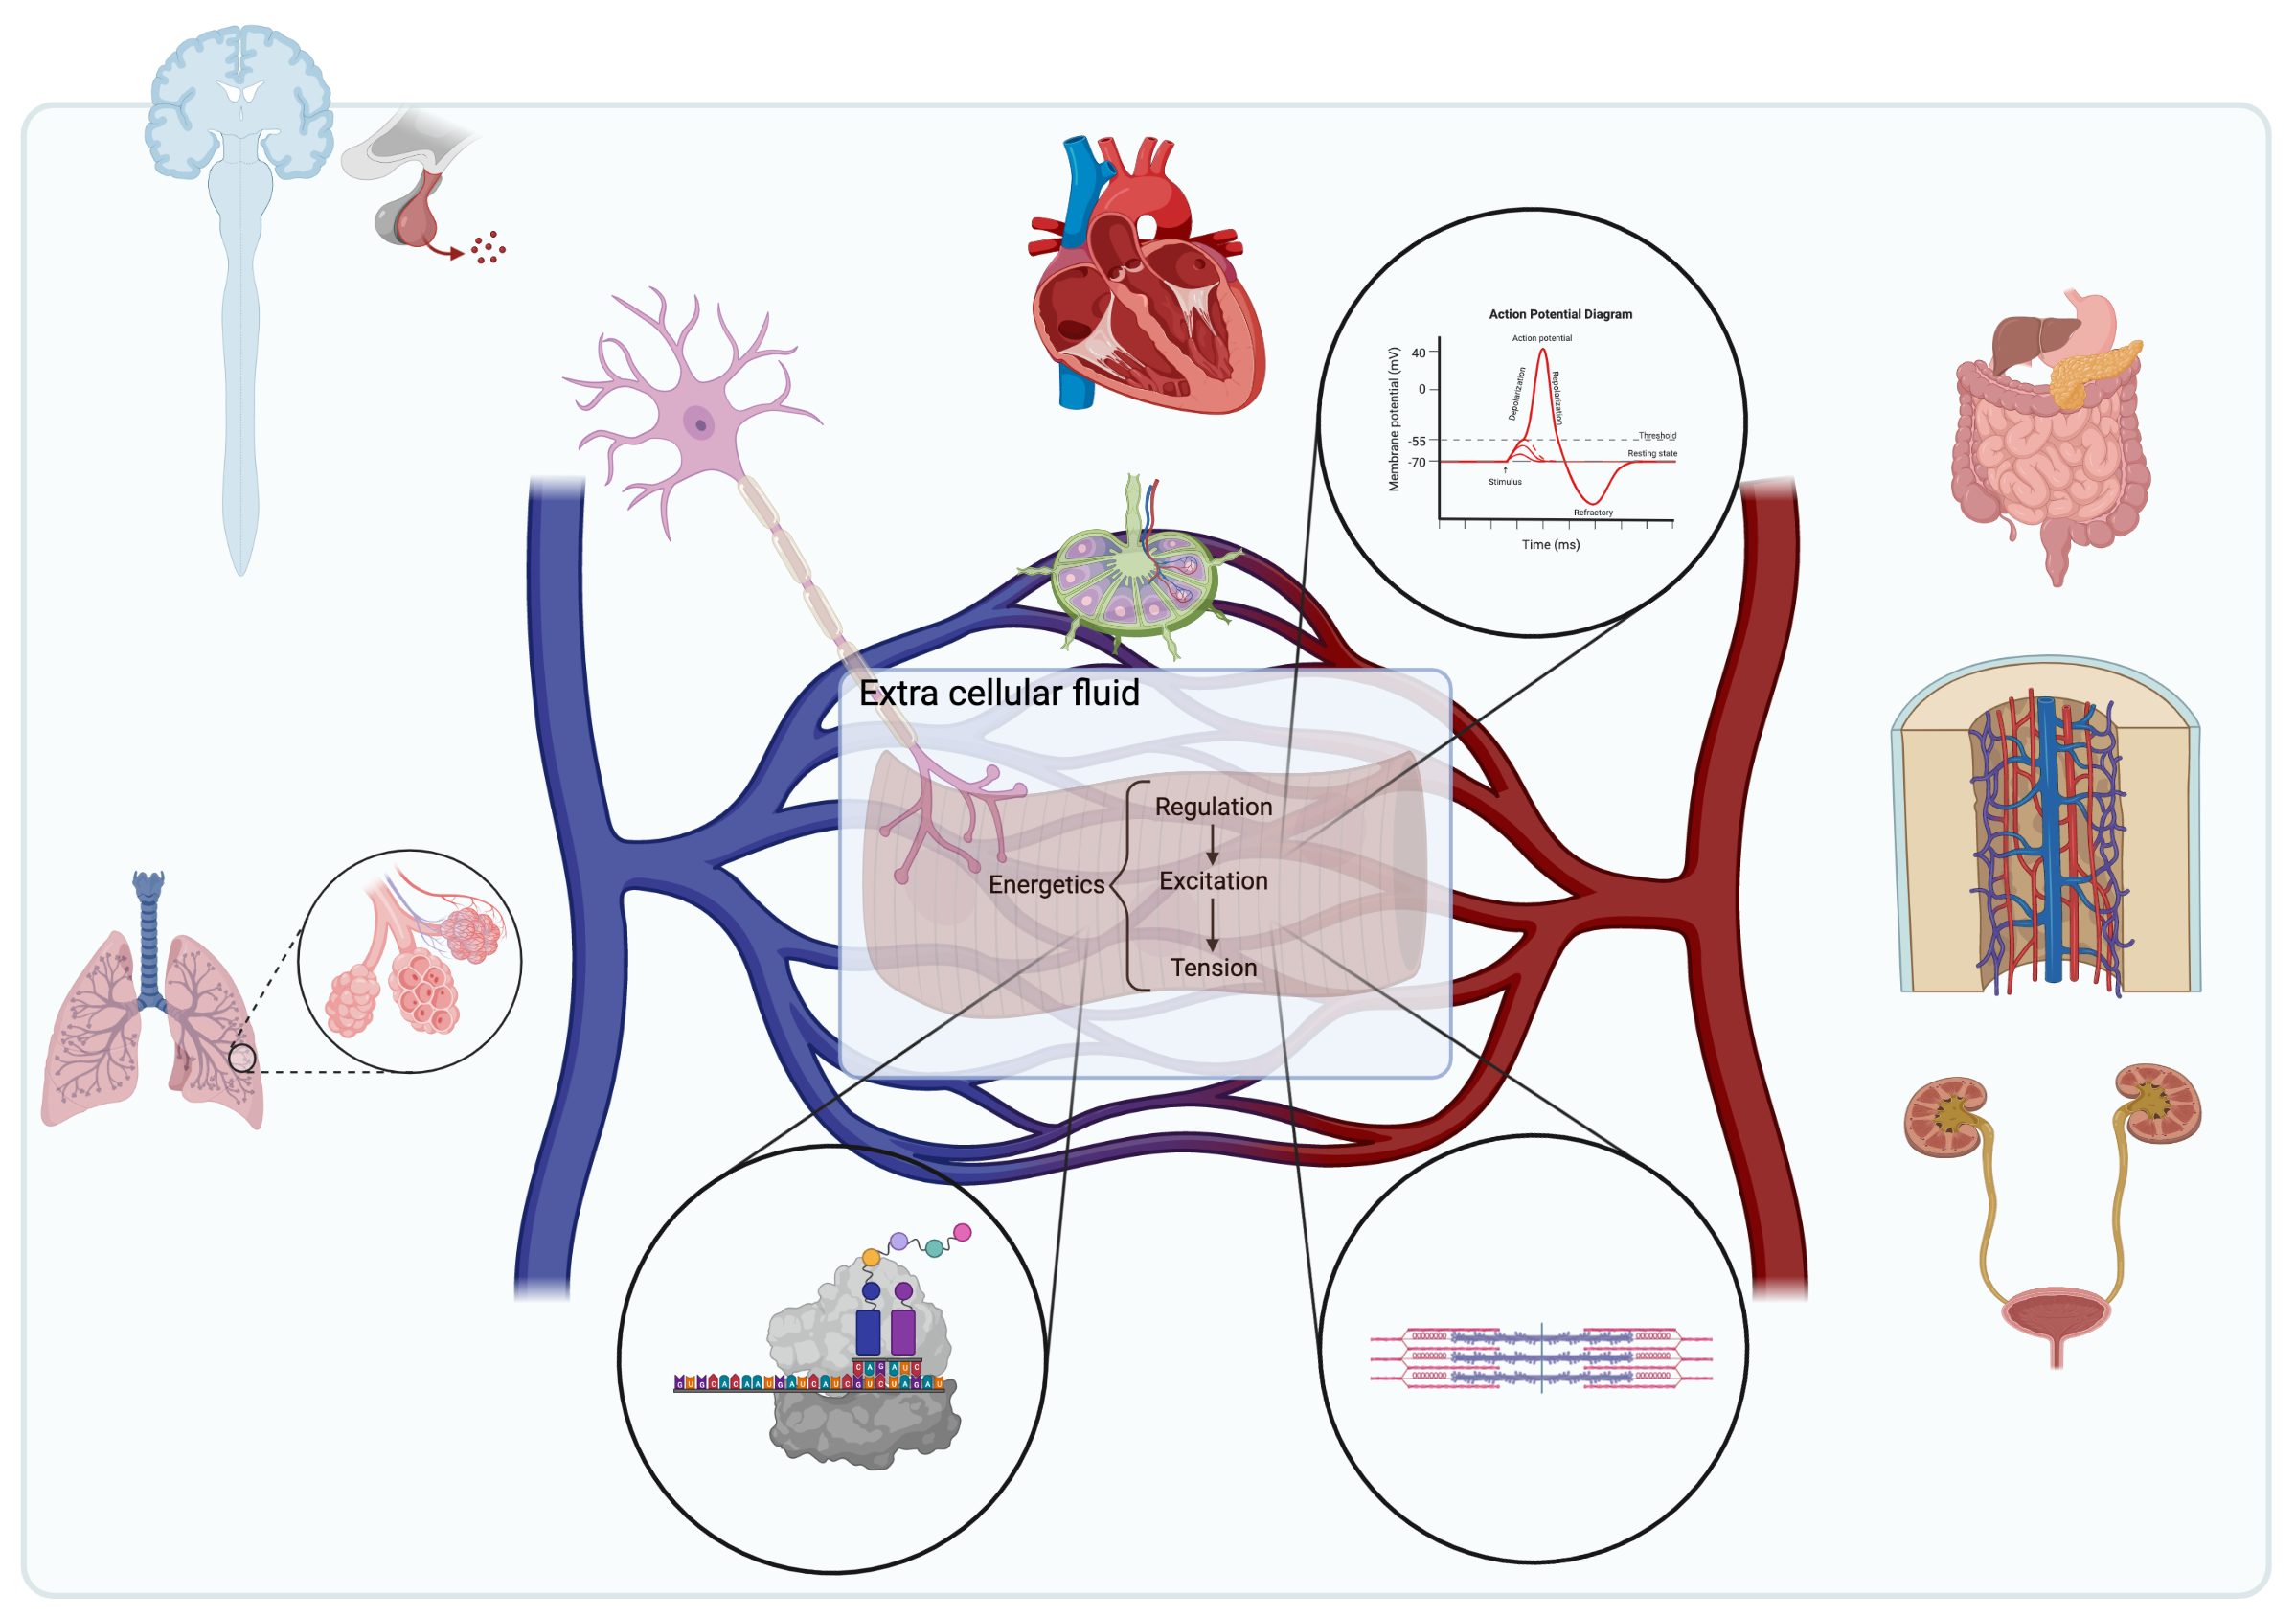
\includegraphics[width=1\linewidth]{./figure/Course_Graphic.png}
    \caption{Muscle Centered Approach \footnotesize{Created with BioRender.com}}
    \label{fig:course_graphic}
\end{figure}

Part I has highlighted the muscle for this muscle centered approach to clinical physiology. Muscle tension produces the forces necessary for movement. Muscle tension is produced with excitation and activation. Excitation, and therefore activation and tension, are regulated by motor units. Muscle tension, activation and excitation all require ATP and therefore the continuous regeneration of ATP. These processes are require an particular intra and extra cellular environment for the muscle fiber. Figure \ref{fig:course_graphic} places the muscle fiber at the center with the chapters of Part I represented as a directed graph. The extracellular electrolytes and availability of substrates such as glucose and fatty acids, the availability of $O_2$ and removal of $CO_2$ all require extra cellular maintenance. The concept of fatigue and the situations causing hypoxia often include what is happening in the muscle fiber, and also what is happening just outside of the muscle fiber. 



Part II is how physiological processes and systems support the muscle as a tension generating system and all that such an act requires. These systems support the muscle tension act by supporting the extra cellular fluid. The first chapter of Part II, Chapter \ref{chp:ecf_microcirculation}, is on Micro-circulation. 

\printbibliography[heading=subbibintoc]


\part{Muscle Support}
% !TEX root = ../notes_template.tex
\chapter{Micro-Circulation}\label{chp:ecf_microcirculation}
Updated on \today
\minitoc

The ECF supports muscle fibers by having the correct resources necessary for muscle function. ECF resources include the correct concentration of ions, the availability of nutrients and molecules such as oxygen. The ECF is also where things moved from the muscles end up until they can be metabolized or removed from the body. Exchange between the ECF and intra-cellular fluid (ICF) is selective for ions, molecules and nutrients but comparatively free for water. The function of muscle fibers depends on the homeostasis of ECF oxygen, carbon dioxide, sodium, potassium, calcium, water, pH, and temperature.
The micro-circulation supports the ECF. Micro-circulation ensures a continuous circulation of the ECF between its two compartments, vascular and interstitial. Water, ions, molecules and nutrients are constantly circulating between the vascular (capillaries and lymphatics) and interstitial compartments of the ECF. 

% 

\vspace{5mm}

\textbf{Objectives include:}
\begin{enumerate}
    \item Explain the basic dependency of muscle fibers on the extra-cellular fluid.
    \item Explain the basic dependency of extra-cellular fluid on the micro-circulation, circulation, renal filtration, respiration, ventilation, digestion, absorption, metabolism and elimination.
    \item Explain the difference between vascular, interstitial and intra cellular fluid.
    \item Explain the role osmosis, osmolarity and osmotic pressure play in micro circulation between ECF-ICF and various situations leading to intra-cellular edema.
    \item Explain the components, roles and implications of the parameters of the filtration equation to explain net filtration and filtration at each end of the capillary.
    \item Use the filtration equation to explain various causes of extra-cellular edema.
    \item Compare and contrast smooth muscle and skeletal muscle.
    \item Explain the underlying mechanism for the effectiveness of compression in edema management.
\end{enumerate}

\section{Muscle Support Overview}

The chapters of Part II are about the supportive environment of the ECF. Every chapter describes a set of functions that serve the purpose of delivering, removing or regulating the contents of the ECF. This chapter focuses on the process of micro circulation of water and filtration of ions, molecules, nutrients and heat between the  vascular compartment of the ECF and the interstitial compartment, the non vascular compartment of the ECF.  

% Type something

Figure \ref{fig:part2_overview} is a graphic representation of the chapters of Part II. Filtration relies on micro-circulation which relies on circulation. Circulation is the flow of blood through the entire circulatory system, covered in Chapter \ref{chp:blood_flow} on Blood Flow. Circulation of blood through the entire body ensures regular mixing of the ECF contents throughout the body. This mixing ensures consistency of ECF contents and a stable environment for all the cells of the body. For example, if blood $Na^+$ concentration is tested, it is properly assumed that concentration is the concentration of $Na^+$ throughout the entire ECF. Circulation also allows that each supporting system contribute - either to adding water, heat, ions, molecules or nutrients to the ECF, or removing by-products from the ECF. Supporting systems are also in communication with one another based on the circulating substances and messages (hormones). For example, if a muscle working at high tension is shuttling lactate into the ECF, it is picked up by the circulation and can then enter other cells (heart, liver, non working muscles) where lactate levels are low. In these cells the lactate can be used to produce an $NADH$ from $NAD^+$, and a pyruvate to proceed into the mitochondria. The circulation is the nationwide transportation and distribution system that gets a package from the local post office to a post office across the country. The micro circulation is the delivery from the local post office to and from a mailbox at an address.

The contents of blood is regulated and supported by renal filtration (kidneys) and endocrine system, covered in Chapter \ref{chp:blood_content} on Blood Volume. The regular circulation of blood through the kidneys involves several mechanisms that selectively filter the blood and in doing so regulate the ECF, and therefore the ICF volume. The regulation of fluid volume includes the regulation of several important ions (electrolytes) and the removal of waste (i.e. urea). Working with the endocrine system the kidneys provide long term regulation of blood pressure, which is important for circulation; as well as red blood cells, which is important for oxygen carrying capacity.

Cellular respiration in the mitochondria is constantly using $O_2$ and producing $CO_2$. These molecules are called gases (blood, alveolar) because their natural state is in the gaseous form. The micro circulation ensures the regular delivery ($O_2)$ and removal ($CO_2$) of these gases from the interstitial fluid. The circulation to the lungs ensures the regular exchanges of these gases with the environment. Blood gases rely on blood flow through the lungs for respiration (gas exchange) between the blood and alveoli, covered in Chapter \ref{chp:blood_oxygen} on Blood Gas. Respiration depends on ventilation, the regular movement of these gases into and out of the lungs with the bulk transport of air. Ventilation is covered in \ref{chp:alveolar_oxygen} on Alveolar Gas. 

Maintaining blood nutrients relies on digestion, absorption, metabolism and elimination by the gastrointestinal organs and the liver. Based on the basic physiological concept of mass balance the regular elimination of water requires the regular intake of water. The regular transformation of the carbon bond energy from carbohydrates and fats requires the regular intake of carbohydrates and fat. The regular use, breakdown and elimination of proteins for cellular functions requires the regular intake of protein. All together these processes are covered in Chapter \ref{chp:blood_nutrients} on Visceral Support.

\begin{figure}[!h]
    \centering
    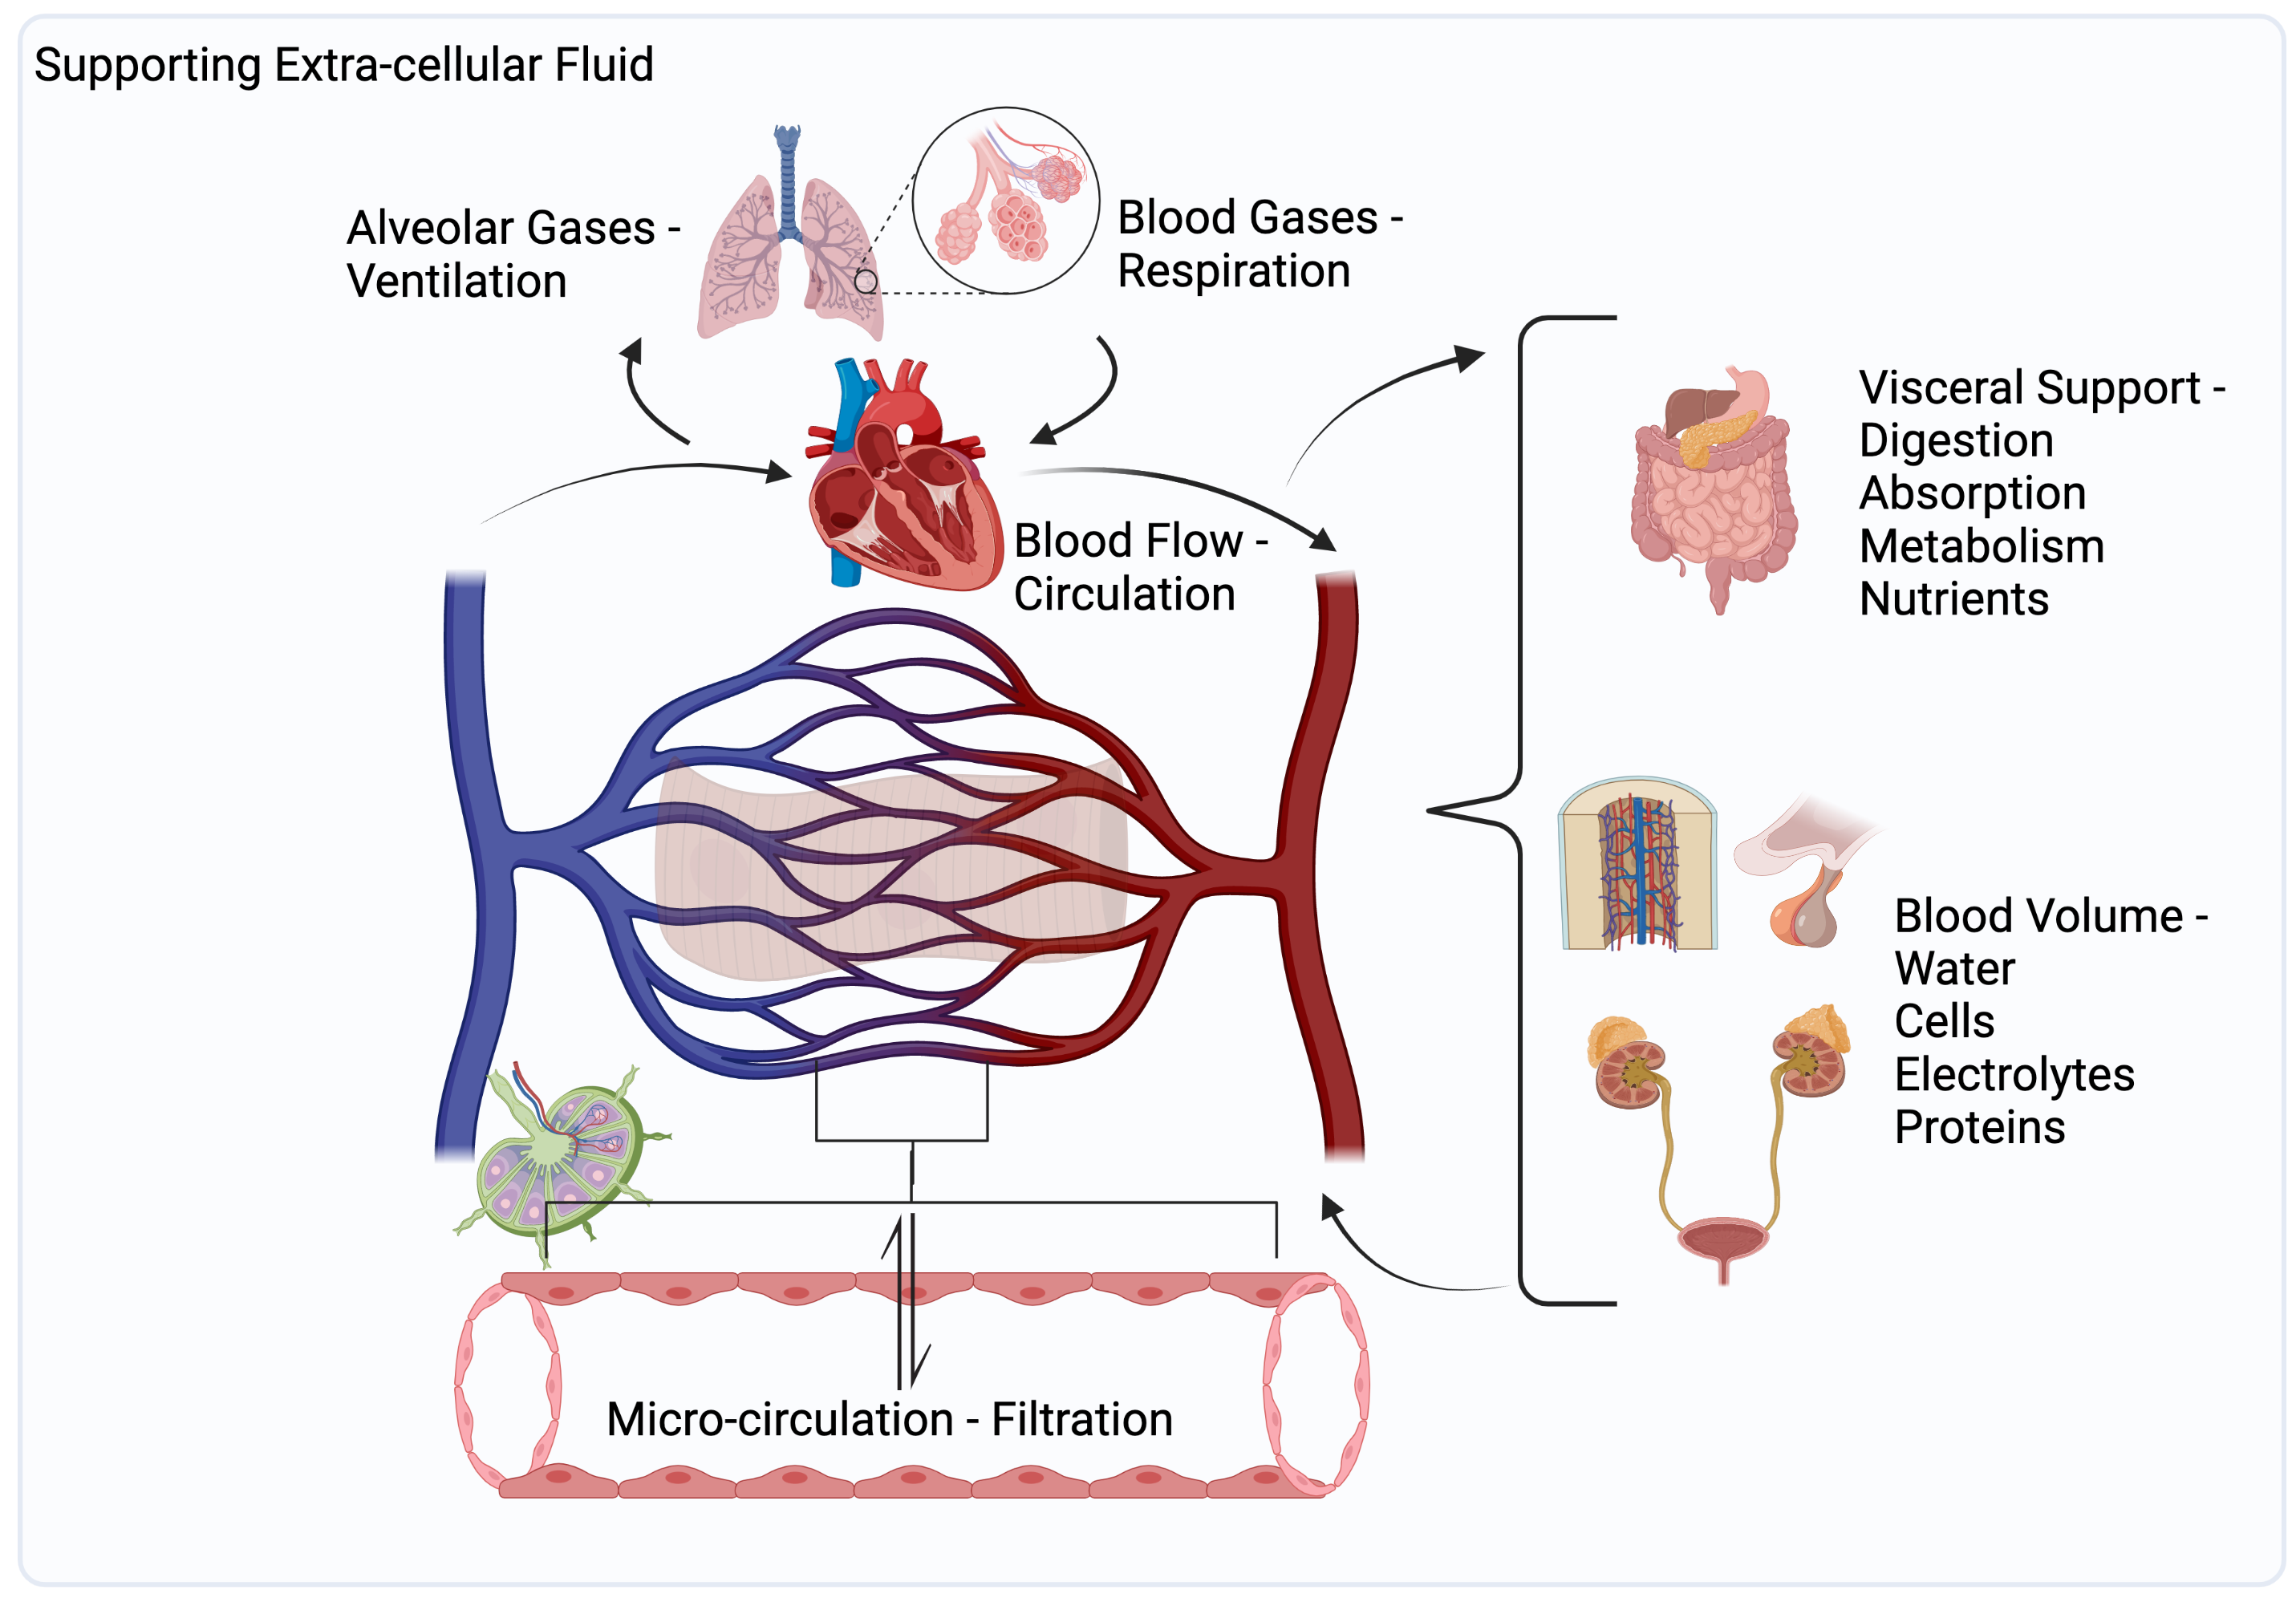
\includegraphics[width=1\linewidth]{./figure/part2_overview.png}
    \caption{Part II: Muscle Support Overview \footnotesize{Created with BioRender.com}}
    \label{fig:part2_overview}
\end{figure}

Together these systems support the ECF and therefore muscle fibers and muscle function. They maintain homeostasis of several important electrolytes (ions, including $H^+$ as measured by pH), nutrients, molecules, water and heat (temperature). The systems are are integrated with several interactions and redundancies to provide support across a wide range of muscle demands in a wide range of circumstances, both good and bad.

One difference between Part I and Part II of the book is that many topics throughout the chapters are in Part II are inherently \textit{Clinical Physiology Connections}. Since the concepts described in Part II are traditional concepts in a clinical physiology course, in many ways these chapters are, in their entirety, clinical physiology connections. As the occasion arises, in pace of \textit{Clinical Physiology Connections} there will be \textit{Muscle Connections} as in this chapter on Smooth Muscle.

\section{Micro Circulation}

Micro-circulation is the continuous movement of ions, nutrients and molecules between the blood plasma (vascular part of ECF) and interstitial fluid. Micro-circulation occurs through the semi permeable capillary membranes in a process called filtration. The capillary membranes allow relatively free passage of water, ions, molecules and  nutrients (other than proteins). The contents of plasma and interstitial fluid is similar other than cell and protein content (particularly red blood cells and albumin), due to an inability of these larger items to pass through the capillary membrane. There are also differences in $O_2$ and $CO_2$ due to the constant exchange with the cell.

Normal values of several important ions, molecules and nutrients are depicted in Figure \ref{fig:ecf}. Vascular and interstitial values are typically equal unless otherwise noted. $O_2$ and $CO_2$ pass easily through both the semipermeable capillary membrane and the semipermeable sarcolemma. There is a relatively large gradient for these molecules that varies due to the muscle fiber energetics. Normal function of circulation, respiration and ventilation at sea level are capable of equilibrating the vascular $O_2$ and $CO_2$ content even extreme high energetic situations.

\begin{figure}[!h]
    \centering
    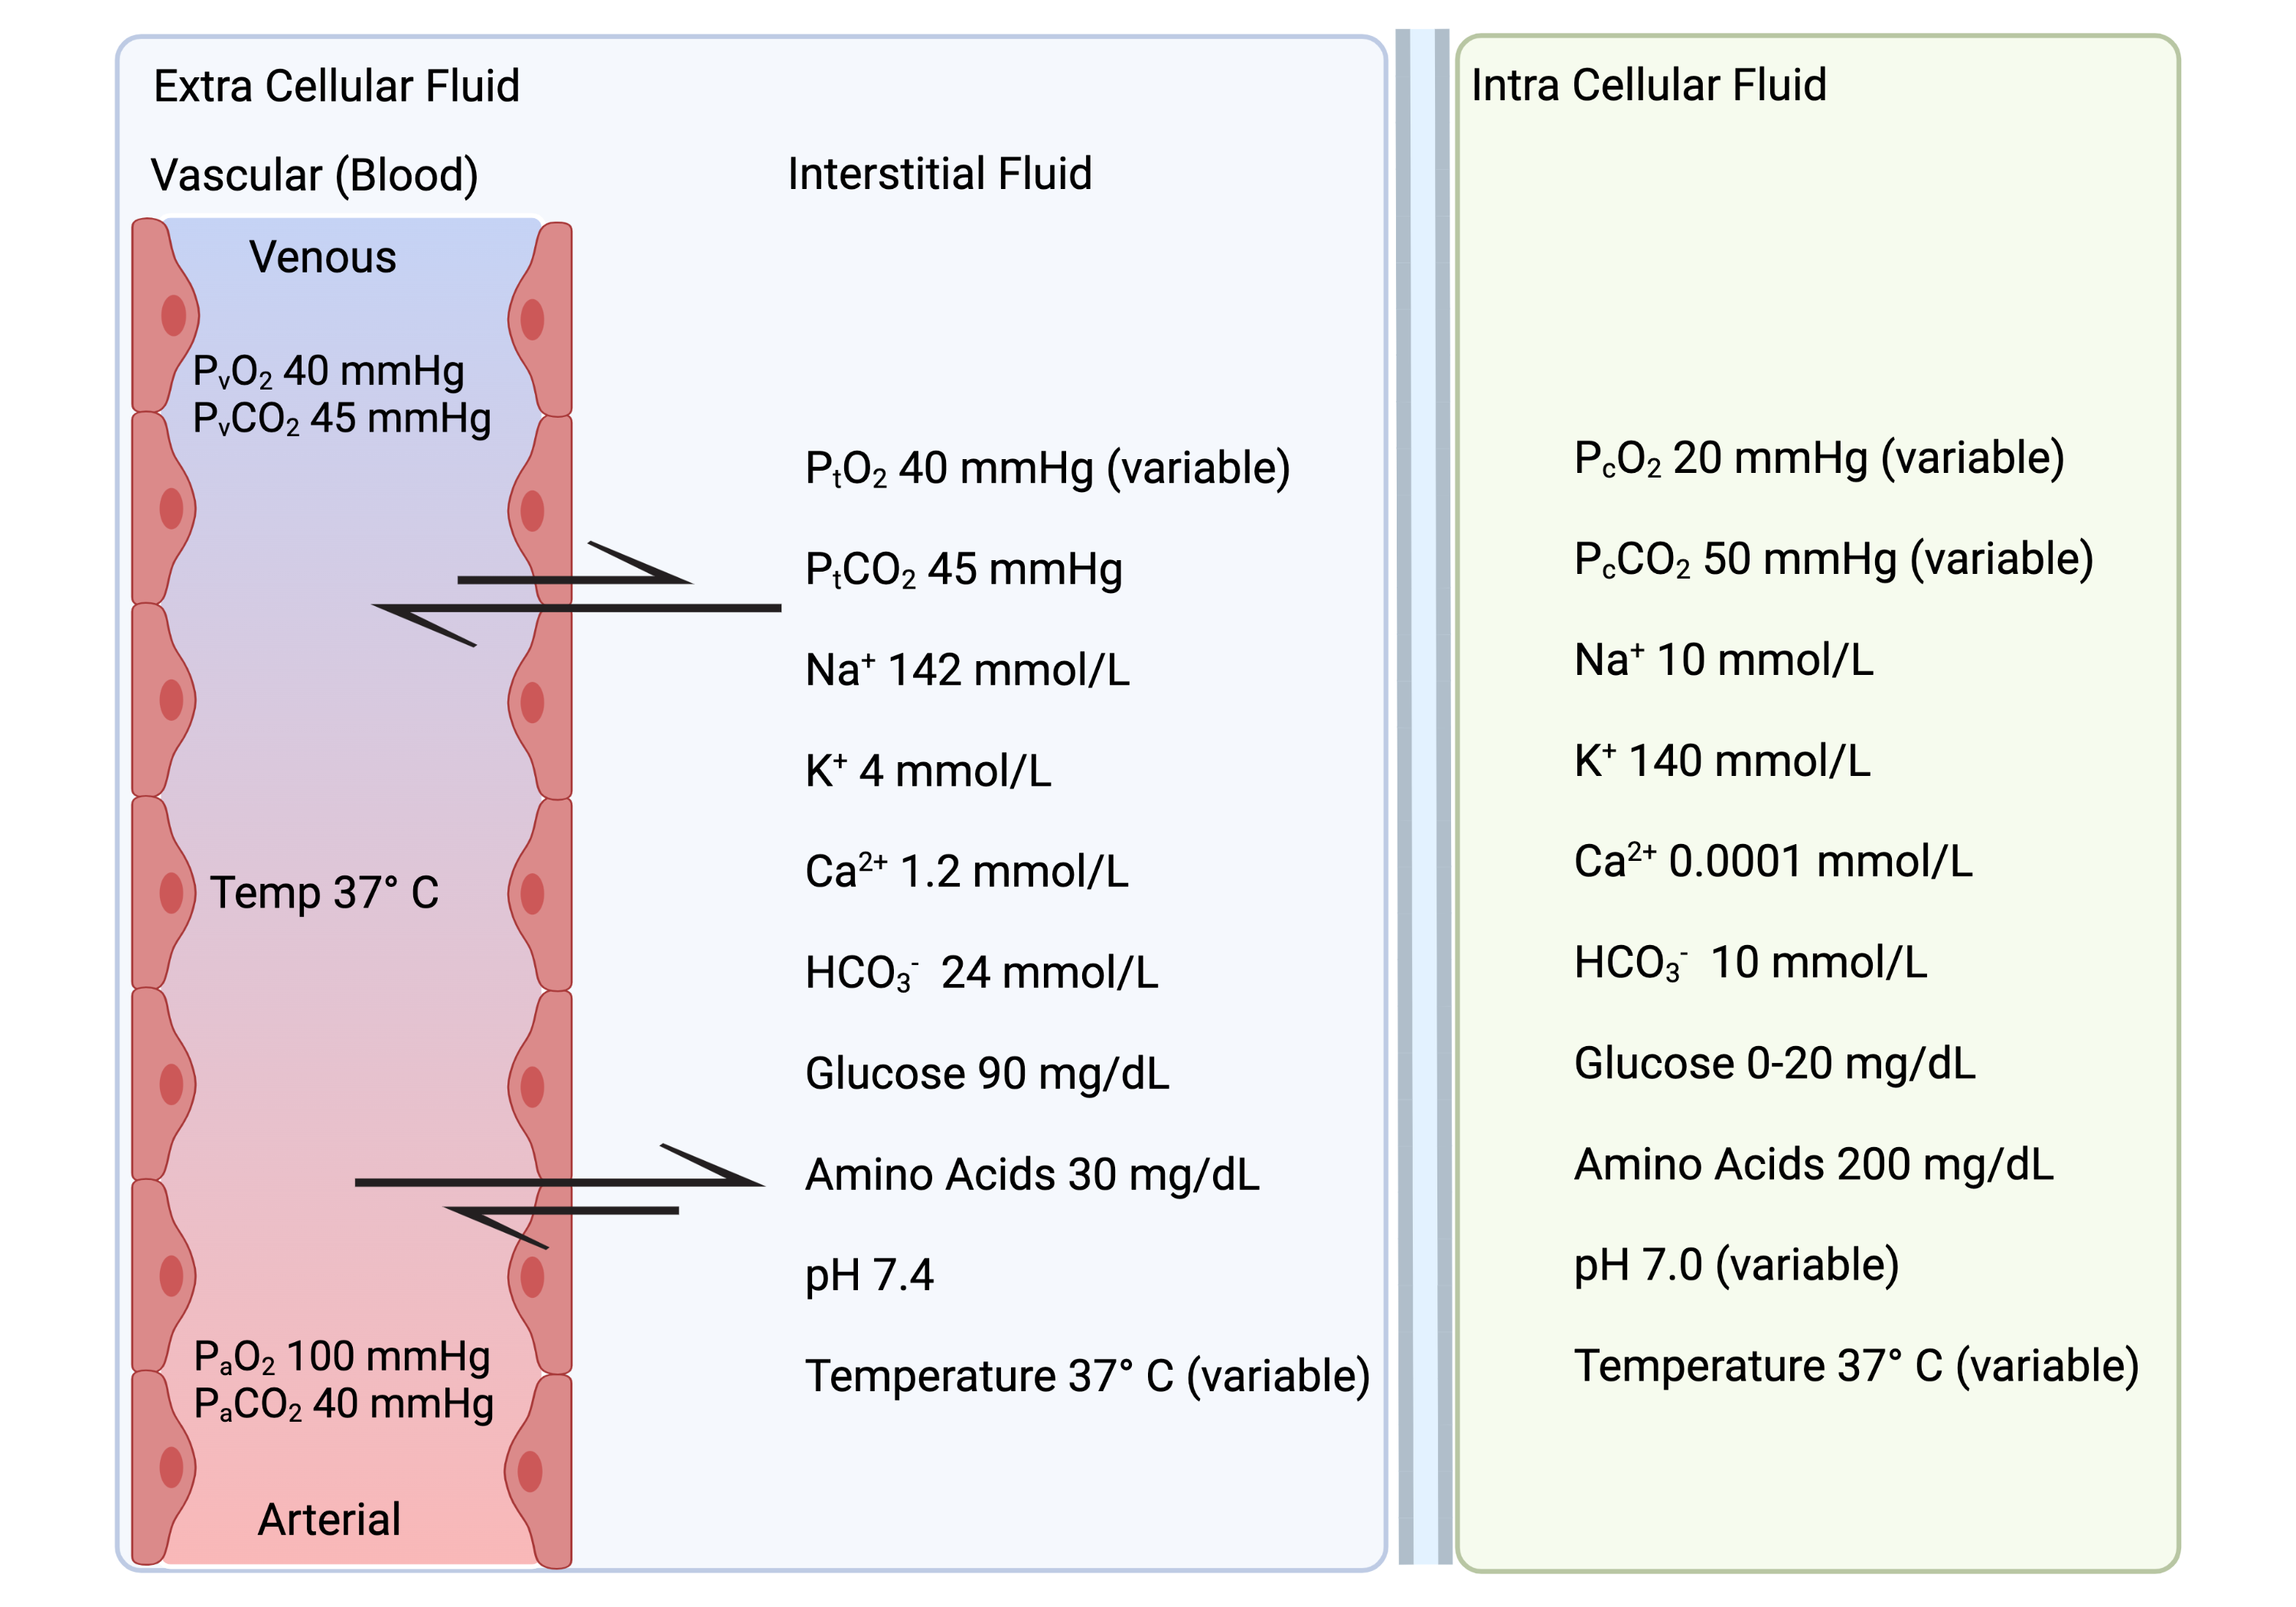
\includegraphics[width=1.0\linewidth]{./figure/ecf.png}
    \caption{Extra-cellular (Vascular \& Interstitial) and Intra-cellular Fluid \footnotesize{Created with BioRender.com}}
    \label{fig:ecf}
\end{figure}

\subsection{Extra Cellular - Intra Cellular Fluid Movement}

Exchange between the interstitial fluid and intracellular fluid occurs through the semi permeable cell membrane (sarcolemma). The sarcolemma restricts movements of ions and even with changes in the permeability for $Na^+$ and $K^+$ during excitation does not change the concentration difference between the interstitial and ICF fluid for these ions (at least under normal circumstances). The sarcolemma regulates the movement of nutrients.  Glucose uptake by a cell is influenced by the activation of the glut4 receptor channel for glucose by insulin. 

Between 50-70\% of an adult body is water. The variation in the percent of the adult body that is water is based on variations in lean (mostly muscle) tissue. In individuals with more muscle (compared to adipose tissue) there is a higher percent of water. Of the total body water approximately 2/3 is intracellular (ICF) and 1/3 is extra cellular (ECF). Since water moves freely between the interstitial and ICF due to a large quantity of aquaporins (water channels) in the cell membrane the balance of ICF and ECF water volume is based largely on solute concentrations and resultant balance of osmotic pressure.

\subsubsection{ECF - ICF Water Volume Balance}

The sarcolemma is permeable to water but not to the ions. The osmolarity between the ECF and ICF determines whether there is net water movement by osmosis and the water (fluid) volume shifts between ECF and ICF. Under steady state conditions the osmolarity between the ECF and ICF is equal. Changes in solute concentration (ions, molecules, nutrients) in the ECF and ICF changes the osmolarity and results in movement of water until osmolarity balance is achieved.

\paragraph{Review of Osmotic Pressure}

At this point most people benefit from a review of these terms and the associated process of osmosis and osmotic pressure. Osmosis is the net movement of water across a selectively permeable membrane caused by a concentration difference across the membrane. Osmotic pressure is the pressure required to prevent osmosis of water through a membrane that is permeable to water but not to the solute (similar concept to an equilibrium potential). The osmotic pressure is an indication of how quickly osmosis occurs (driving force); and osmosis does not occur if there is no osmotic pressure gradient. Osmotic pressure is exerted by particles and is determined by the number of particles per unit volume of fluid. 

The osmole (Osm) expresses solute concentration in terms of the number of particles. An Osm is the number of moles of solute that contribute to the osmotic pressure of a solution. Osmolarity refers to the number of osmoles in a volume (Liter (L)) of solvent. Osmolarlity = Osm / L. Osmolarity is proportional to the milli osmoles / L as well (mOsm/L).

Osmotic pressure ($\pi$) is directly proportional osmolarity (concentration in Osm in a volume (L) of solvent) ($C$); the ideal gas constant ($R$); and absolute temperature ($K = 310^{\circ}$ at body temperature) in the equation: $\pi = C \cdot R \cdot T$. Since $R$ is a constant, and $K$ in the body varies within a relatively narrow boundary, the osmotic pressure is determined by the osmolarity (Osm/L). At body temperature each 1 mOsm/L (milli osmole per liter) results in approximately 19.3 mmHg of osmotic pressure. In Figure \ref{fig:osmotic_pressure} the solution on the left has 1 mOsm/L more osmolarity. At body temperature this means 19.3 mmHg of pressure is required to stop the movement of water. Differences in osmolarity due to differences in solute concentration across the sarcolemma results in osmosis of water until there are no differences in osmolarity.

\begin{figure}[!h]
    \centering
    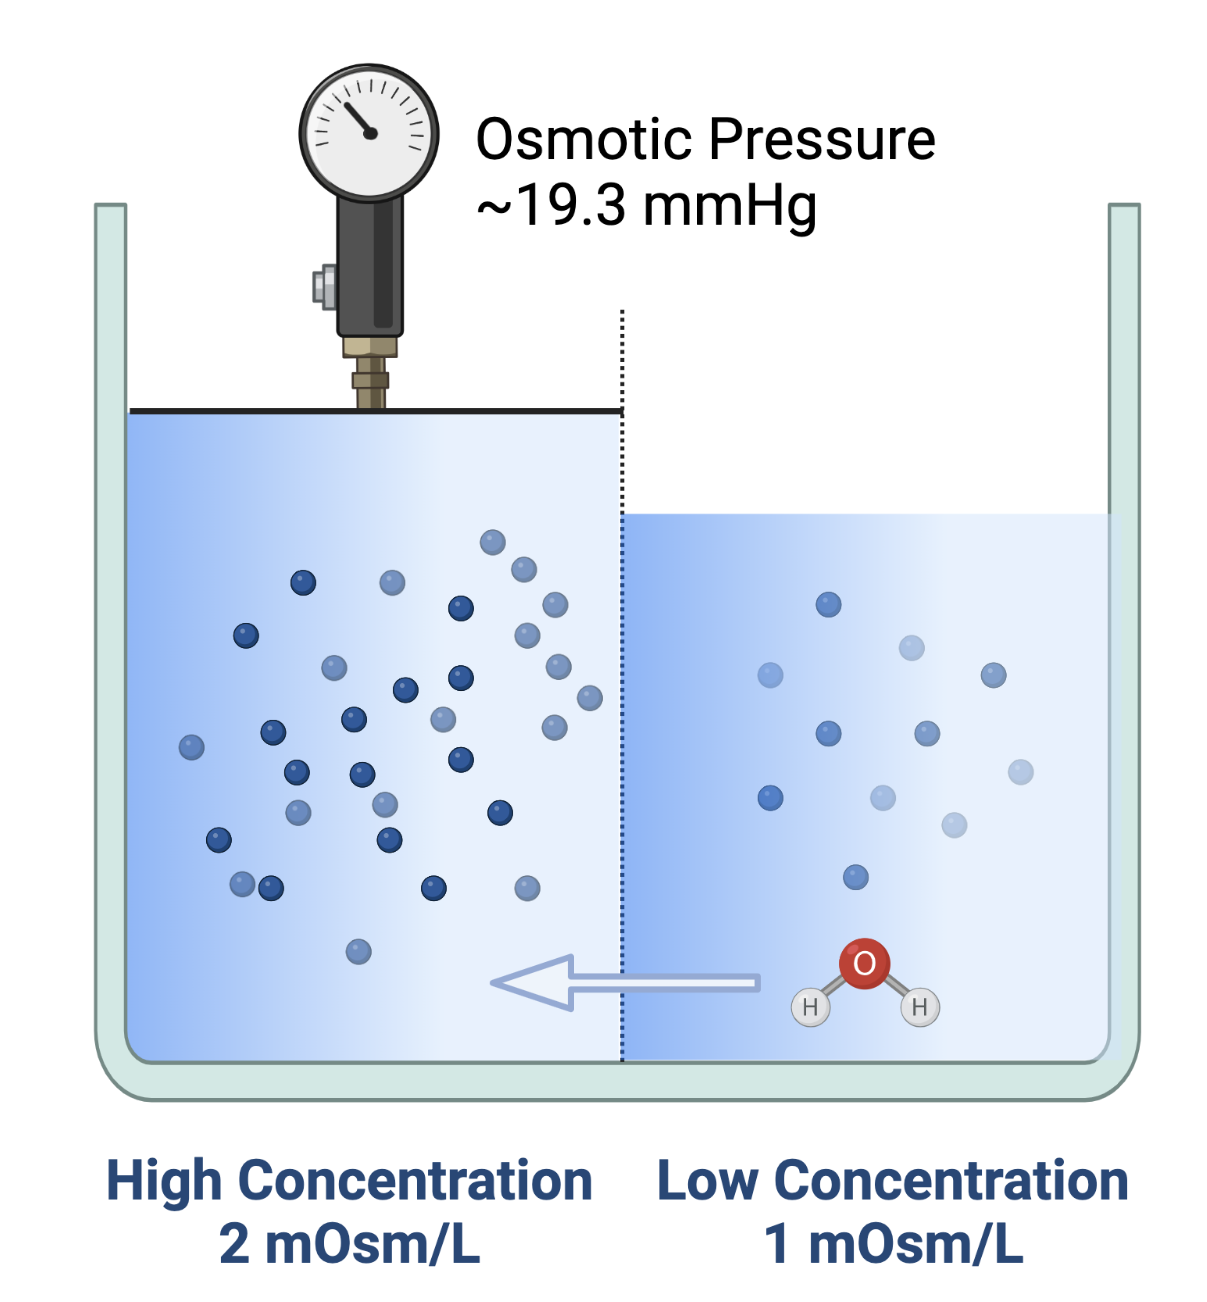
\includegraphics[width=0.5\linewidth]{./figure/osmotic_pressure.png}
    \caption{Osmotic Pressure \footnotesize{(Created with BioRender.com)}}
    \label{fig:osmotic_pressure}
\end{figure}

Since water moves freely across the sarcolemma osmosis occurs and balances the osmolarity of the ICF with that of the ECF. When the osmolarity of ECF and ICF are equal there is no osmosis or net movement of water across the membrane since the osmotic pressures cancel each other out.

The total intake of water and ions (electrolytes) are carefully matched by equal outputs from the body to prevent fluid volumes and ion concentrations from fluctuating beyond acceptable ranges (mass balance, and homeostasis). There are times when there are differences between intake and output of water and ions that eventually must be remedied. Small shifts in water between ECF and ICF ensure that both compartments have the water required and maintain appropriate ion concentrations.

These shifts typically start with changes to the ECF. It is usually the ECF that we are adding, or removing, water and ions to, or from, (ingestion, absorption, renal filtration). Water and ions are also removed from ECF in the kidneys, the colon (small amount under normal circumstances) and water is removed from ventilation.  These changes in water volume change the concentration and therefore osmolarity of ECF. 

% All things that enter the ICF do so from the ECF, the ICF does not typically have changes to osmolarity that are not provoked by the ECF first. There are some circumstances discussed below that ICF osmolarity may change in response to abnormalities in ICF $K^+$ concentration. 

The response to changes in osmolarity between the ECF and ICF is movement of water by osmosis until there is once again equalize the osmolarity. Large water intakes to the ECF such as large water intake or IV infusions; or decreases (dehydration) associated with sweating, GI fluid loss, or excessive urine formation by the kidneys (i.e. in diabetes mellitus) change the ECF water volume. If these changes alter the osmolarity of the ECF then water will pass between ECF and ICF until osmolarity is equalized.

Figure \ref{fig:iso_hypo_hypertonic} depicts the changes that would occur to the osmolarity with the addition of a volume of isotonic (same osmolarity), hypotonic (lower osmolarity), and hypertonic (higher osmolarity) solution to the ECF.

\begin{figure}[!h]
    \centering
    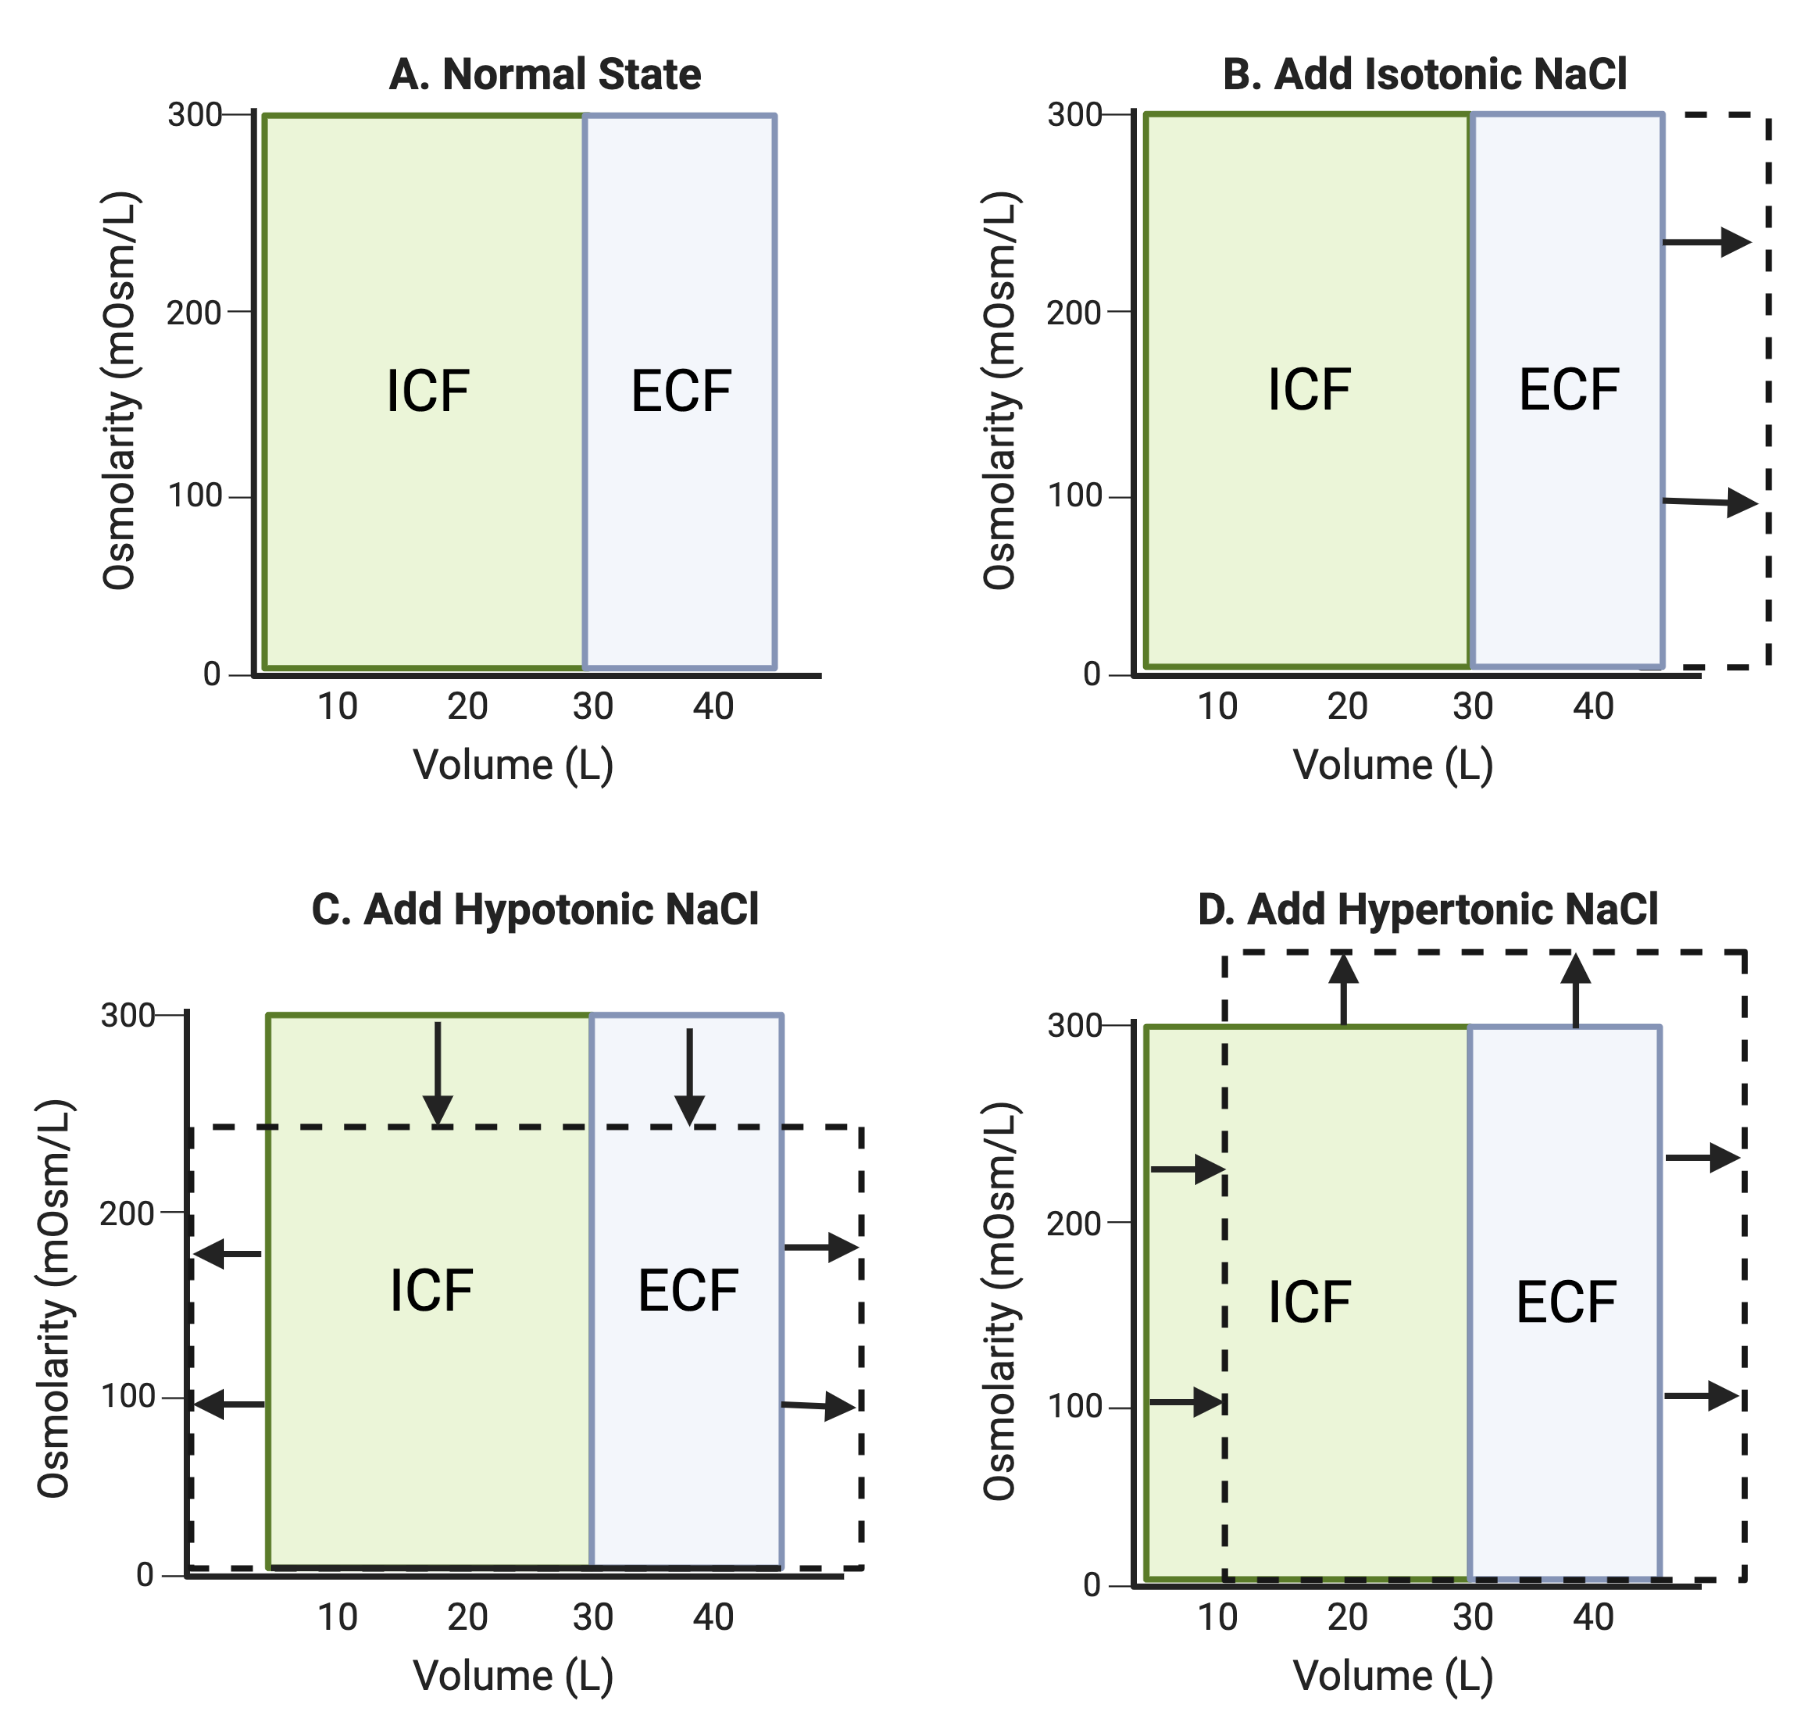
\includegraphics[width=0.7\linewidth]{./figure/iso_hypo_hypertonic.png}
    \caption{Impact of ECF Infusions of Iso, Hypo and Hypertonic Solutions (See text for details) \footnotesize{(Created with BioRender.com)}}
    \label{fig:iso_hypo_hypertonic}
\end{figure}


\begin{itemize}
    \item Adding an isotonic solution to ECF does not change osmolarity of the ECF so there is no osmosis (no change in net water movement). The end result is an increase in ECF volume but no change to ICF volume (See Figure \ref{fig:iso_hypo_hypertonic} B).
    \item Adding a hypotonic solution to ECF decreases the osmolarity of ECF and results in osmosis of water into the cells (ICF) and increases ICF volume. This continues until the osmolarity of ICF decreases and the concentration of ECF increases until the osmolarity of both compartments are equal which stops the net flow of water into the ICF. The overall effect is increased ICF and ECF volume, and decreased ICF and ECF osmolarity (See Figure \ref{fig:iso_hypo_hypertonic} C). 
    \item Adding a hypertonic solution to ECF increases the osmolarity of ECF and results in osmosis of water out of the cells (ICF) and decreases ICF volume. This continues until the osmolarity of ICF increases and osmolarity of both compartments are equal which stops the net flow of water out of the ICF. The overall effect is decreased ICF volume and increased ECF volume; and an increase of osmolarity of both ICF and ECF See Figure \ref{fig:iso_hypo_hypertonic} D).
\end{itemize}

\paragraph{Importance of Osmosis to Muscle Excitation}

Changes in the osmolarity of the ECF and ICF are based on the concentration of these solutions. The concentration changes with changes to the water volume or changes to the amount of solute. A hypertonic solution therefore increases the concentration of $Na^+$ in both the ECF and ICF, but retains the concentration gradient. A hypotonic solution decreases the concentration of $Na^+$ in the ECF and ICF, but does not change the concentration gradient. Since the concentration gradient of $Na^+$ (and all ions) across the sarcolemma is critical to excitation, it should be clear that these osmotic pressure directed fluctuations to water volume serve an important buffer capacity to maintain these ion concentration gradients. Dehydration, a reduction in water volume, ultimately results in a slightly higher concentration of ions, but this higher concentration is balanced between the ECF and the ICF, so gradients are kept constant.
Ion abnormalities exist (electrolyte imbalances), but they do not have as profound an impact as they would if water did not move freely between ECF and ICF to normalize concentration gradients. 

\paragraph{Intra Cellular Edema}

Intra cellular edema is when there is increased fluid in the intra cellular space. Edema of the ICF can occur locally or systemically. As described above, ICF edema can occur with the addition of a hypotonic solution to the ECF (See Figure \ref{fig:iso_hypo_hypertonic} C). In general, any situation that reduces the osmolarity of the ECF can result in ICF edema. Hyponatremia (low ECF $Na^+$) reduces the ECF osmolarity, which results in a fluid shift from ECF into the ICF until the osmolarity between these compartment equalizes. This is an example of systemic ICF edema (effects all cells). Since this fluid shift from ECF to ICF is systemic it tends to be self limiting - the osmolarity between the ECF and ICF will eventually reach a balance.

Local depression of energetic systems which can occur due to a lack of adequate nutrition or $O_2$ (i.e. hypoxia) can increase the osmolarity of the cells and pull more water (locally) in from the ECF. In this situation there are two contributing problems. First, is a local depression of the $Na^+/K^+$-ATPase pumps (for lack of ATP) which leads to an accumulation of $Na^+$ inside the cell. Second, the accumulation of lactate and $H^+$ in the cell cannot be balanced by the removal. Keep in mind, this situation entails depression of energetic systems due to a lack of oxygen. If that lack of oxygen cannot be remedied with a reduction in ATP demand then the imbalance will persist until the cell dies. Cell death occurs when the cell membrane is no longer intact. The above scenario includes an acid pH (damaging to the cell membrane) and cellular edema (damaging to the cell membrane). The increase in cellular osmolarity (since it is a local occurrence) does not (or cannot) lead to a balance of osmolarity between the ECF and ICF because it is not systemic. The local cells cannot pull in enough fluid to alter the osmolarity of the entire ECF.

Extracellular edema can also cause intracellular edema if the extra cellular edema lowers the ECF osmolarity. Similar to adding a hypotonic solution to the ECF or in the case above of hyponatremia, with reduced ECF osmolarity the ICF osmolarity would pull water into cells until the osmolarity is equalized. A hypotonic solution is water (isotonic is water with 0.9\% NaCl or 5\% glucose). Adding too much water to the ECF (over drinking water) before adequate renal filtration and secretion can occur can lead to extra cellular edema and reduced ECF osmolarity. Note, problems with renal filtration and secretion (i.e. kidney failure) does not create this problem because there is also a build up of urea and other solutes in the ECF. So kidney failure does not cause a reduction in osmolarity of the ECF, but might cause an increase in the osmolarity of the ECF. 

\subsection{Extra cellular Values \& Ranges}

Table \ref{table:ecf_value_ranges} provides normal values and ranges and non lethal limits for several important components of the ECF.  The wide normal ranges and non lethal limit ranges is a good example of the degree of overall robustness. Moving outside of a range without an easy temporary explanation (such as low $P_v O_2$ in response to exercise) is an indication that something is wrong. But even when something is wrong, the body adjusts and even large deviations in normal values are tolerated before the changes become lethal. Several of these components of the ECF have larger non lethal limits in one direction. For example, $P_v O_2$ can increase tremendously (if given a large amount of oxygen in hyperbaric (high pressure) systems) before it becomes lethal. The criteria for lethal for these values is death. Some of the secondary effects may lead to premature death. 

\begin{table}[h!]
\centering
\begin{tabular}{||c c c c||} 
 \hline
Value & Normal Value & Range & Non-Lethal Limit\\ [0.5ex] 
 \hline\hline
 $P_v O_2$ (mmHg) & 40  & 25-40 & 10-1000 \\
 $P_v CO_2$ (mmHg) & 45 & 41-51 & 5 - 80\\ 
 $Na^+$ (mmol/L) & 142 & 135 - 145 & 115 - 175\\
 $K^+$  (mmol/L) & 4.2 & 3.5 - 5.3 & 1.5 - 9.0\\ 
 $Ca^{2+}$ (mmol/L) & 1.2 & 1.0 - 1.4 & 0.5 - 2.0 \\
 $HCO_3 ^-$ (mmol/L)& 24 & 22 - 29 & 8 - 45 \\
 Glucose (mg/dL)& 90 & 70 - 115 & 20 - 1500 \\
 Acid-Base (pH) & 7.4 & 7.3 - 7.5 & 6.9 - 8.0 \\
 Temperature F (C) & 98.6 (37) & 98-98.8 (37) & 65-110 (18.3-43.3)\\[1ex] 
 \hline
\end{tabular}
\caption{Normal Range and Non Lethal Limits of Values in ECF (\footnotesize{Data from \cite{feher_quantitative_2017}})}
\label{table:ecf_value_ranges}
\end{table}

For example, while a $Na^+$ value of 165 mmol/L is within the non lethal limit. This concentration of $Na^+$ is buffered by the movement of water that would occur due to changes in the osmolarity of the ECF so its impact on the concentration is not as great as it may seem. But with such a high concentration it would be associated with, amongst other signs and symptoms of hypernatremia, a high blood volume and therefore high blood pressure despite attempts to maintain normal blood pressure. The elevated blood pressure can then lead to premature death.  Tolerance for temperature is greater with cold than with heat. With heat proteins denature and metabolic functions cannot be catalyzed. With decreased temperature reactions slow down from reduced kinetic energy, but at least the enzymes (proteins) are functioning. 


\subsection{Oxygen \& Carbon Dioxide}

The gradient for $O_2$ from the vascular fluid into the cell exists because the cell is constantly utilizing $O_2$. The gradient for $CO_2$ from the cell to the vascular fluid exists since the cell is constantly producing $CO_2$. The other gradient for $O_2$ and $CO_2$ depicted in Figure \ref{fig:ecf} is from the arterial end of the capillary to the venous end of the capillary. As shown, with healthy capillaries, normal capillary blood flow and normal blood the vascular $O_2$ and $CO_2$ partial pressure equilibrate by the time blood reaches the venous end of the capillary. The cellular and interstitial partial pressure for oxygen ($P_c O_2$ \& $P_t O_2$) are variable based on how much $O_2$ is being consumed in the muscle fiber, which is dependent on the rate of ATP regeneration occurring in electron transport (ETC). With a higher than resting ATP regeneration in ETC the $P_c O_2$ will drop, which drops the $P_t O_2$ below 40 mmHg, and then the partial pressure of oxygen at the venous end $P_v O_2$ of the capillary will also drop. $P_v O_2$ will equilibrate to $P_t O_2$. However, the $P_a O_2$ will remain at 100 mmHg as long as the circulation and pulmonary systems are providing the additional support that is required.

Similarly, for ETC to be regenerating ATP at a higher rate, the citric acid cycle (TCA) has to be functioning at a higher rate and thus producing more $CO_2$. This results in a higher $P_c CO_2$. However, because $P_t CO_2$ and $P_v CO_2$ equilibrate, as long as the circulation and pulmonary systems are providing the additional support that is required there will not be an increase in either $P_t CO_2$ or $P_v CO_2$. The difference between arterial $O_2$ and venous $O_2$ is an important indicator of how much $O_2$ is being consumed. How much $O_2$ is being consumed is an indicator of metabolism and energetic demands from rest to peak exercise. This relationship is captured in the Fick Equation discussed in Chapter \ref{chp:fick_equation}:

\begin{equation}
    \dot{V}O_2 = \dot{Q} \cdot (a-v)O_2
    \label{FicksEquation}
\end{equation}


\subsection{Temperature}

Temperature is heat unless there is a temperature of 0 degrees Kelvin. Heat is a byproduct of all energetic transformations, including regenerating ATP and hydrolyzing ATP. At rest, temperature in muscle fiber tends to equilibrate (or be slightly lower) with that of the body because the flow of heat from the fibers into the ECF is moved to the blood and out of the region. Some of the heat also dissipates through the ECF and tissues across the temperature gradient directly out of the body. When core body temperature falls, a reflex action is to shiver, which utilizes muscle activity to generate more heat for sharing with the rest of the body through the transport of ECF. When muscle temperature rises during activity, the circulation of blood carries much of that heat away from the muscle for dissipation throughout the body. As heat rises, more of the circulation is sent to the skin to facilitate this process.

Temperature of muscles varies more than core temperature. While core temperature is highly regulated at 37 degrees Celsius muscles in the extremities, and more so the distal extremities, can vary from as high as 40 degrees in a hot environment to as low as 20 degrees in the cold. Muscle function when muscle temperature is less than 37 degrees impacts the rate of tension development and the rate of tension recovery (relaxation). At the extreme of 22 degrees a the rate of tension development and recovery is approximately 25\% of that at 37 degrees \cite{jones_skeletal_2006}. This is thought to be due primarily to the dependency on these rates on kinetic energy of moving molecules throughout the chain of events from excitation to activation. The overall impact is that reductions in muscle temperature has a greater impact on high power activities which are dependent on the rate of tension development and recovery.

\subsection{Acid Base (pH)}

Intra cellular fluid has several buffering systems for regulating pH through a wide range of energetic rates and thus do not, in resting or even low to moderate energetic situations, send $H^+$ ions out of the sarcoplasm for acid base balance. In situations that force the utilization of the glycogen $\rightarrow$ lactate pathway such as a high ATP demand or low ETC capacity, lactate (lactic acid) removes excessive $H^+$ ions from the sarcoplasm to the ECF which can then be circulated to other cells for recycling. But this lactate shuttling is not perfect and intra cellular pH can drop if those situations are not balanced.
There are several processes involved with the regulation of ECF acid base balance (pH). Each is presented in the upcoming chapters such as buffers in the blood and through filtration in the kidneys (Chapter \ref{chp:blood_content}, and respiration Chapter \ref{chp:blood_oxygen}).


\section{Filtration}

Micro-circulation relies on filtration between the ECF vascular and interstitial compartments. Filtration occurs through capillary membranes. It includes the flow and exchange of water, ions, molecules and some nutrients (glucose, fatty acids, amino acids). Larger items such as proteins (albumin) and blood cells do not normally filtrate through the capillary membranes. However, in certain circumstances white blood cells, as part of an immune response, will leave the vascular compartment and enter the interstitial fluid.

There are two pressure gradients that drive filtration: osmotic and hydrostatic pressure. Osmolarity creates osmotic pressure that has the net effect movement of water and solutes between the vascular and interstitial compartments. The osmolarity between the vascular fluid and interstitial fluid is one driving force for filtration. The second pressure gradient is hydrostatic pressure (fluid pressure). 

\subsection{Hydrostatic pressure}
Hydrostatic pressure is the force that the fluids exert on the walls of the space they are in, and is related to the size of that space (volume) in and the compliance of the walls of that space.\footnotemark\footnotetext{Pressure is also related to temperature, but varies much more with volume and compliance in the human body than with temperature given the relative stability of temperature throughout the body.} Pressure, volume and compliance are related by the equations (C = compliance, V = volume, P = pressure, $\Delta$ = delta meaning "change in" ):

\begin{equation}
    C = \frac{\Delta V}{\Delta P}
    \label{Compliance}
\end{equation}
\begin{equation}
    \frac{1}{\Delta P} = \frac{C}{\Delta V}
    \label{InversePressure}
\end{equation}
\begin{equation}
    \Delta P = \frac{\Delta V}{C}
    \label{Pressure}
\end{equation}

Compliance is determined by the change in pressure to change in volume (Equation \ref{Compliance}). It is useful to consider how changes in characteristics of a structure change its compliance and then influence $\Delta$ pressure with the assumption of a stable volume, or the influence on volume with the assumption of a stable pressure. As can be seen in equations \ref{InversePressure} and \ref{Pressure}, compliance and $\Delta$ pressure are inversely proportional to one another. Compliance of a tissue (or compartment which in the body is created by tissue) is inversely proportional to stiffness. Fibrosis, which occurs when scar tissue replaces normal tissue in response to injury or inflammation, makes the tissue more stiff and less compliant.

The volume of all capillaries is related to the sum of their cross sectional area. The volume of one capillary is related to its cross sectional area. The cross sectional area is determined by the radius. The radius also influences resistance to flow. And flow influences the amount of fluid entering and exiting. These relationships are complicated, in part, because the radius of the capillaries influences pressure both changing cross sectional area and volume, and by changing resistance to flow. The effect of these relationships is that changing a capillary radius, or the total capillary cross sectional area, has a powerful, and complicated, effect on hydrostatic pressure in the capillaries.


\subsection{Capillary Blood Flow}

The capillaries have a thin endothelial membrane that does not include smooth muscle. Without smooth muscle the radius of a capillary is based on its structure which influences its compliance and the amount of blood flowing into and out of the capillary (volume). Blood flow into the capillaries is regulated by local and central (neuroendocrine) factors. Changing the radius of the arterioles (vessels that flow into capillaries) and pre-capillary sphincters changes the volume of blood entering the capillaries (Figure \ref{fig:capillaries}). Blood flow out of the capillaries is also regulated by local and neuroendocrine factors. However, the venuoles (vessels capillary blood flows into) have a less developed smooth muscle layer than arterioles and therefore influence less effect on the radius of the venuoles. Venuoles, and the entire venous system, have much higher compliance and are described as a low pressure system. This helps to ensure that flow proceeds through the capillaries from the lower compliance (higher pressure) arterial circulation to the higher compliance (lower pressure) venous circulation. Neuroendocrine control of the capillary blood flow is from the sympathetic branch of the autonomic system. Neural and endocrine influences are exerted through the catecholamines (epinephrine and norepinepherine). The effect of catecholamines is vasoconstriction. But this effect is overridden locally as needed. 

The volume of blood in the capillaries changes by changing the flow of blood into and out of the capillaries. A strong local determinant of blood flow, that overrides sympathetic vasoconstriction, are energetic byproducts that indicate the need for $O_2$ such as interstitial $O_2$ being low, $CO_2$ being high, a drop in pH and a rise in temperature. All of these changes, locally, promote dilation of arterioles, pre-capillary sphincters and venuoles. In this situation the increased blood flow generally does not increase the capillary hydrostatic pressure because flow into and out of the capillary is balanced and associated with vasodilation. If blood flow to capillaries increases the capillary blood volume beyond its normal range of compliance then hydrostatic pressure can increase which may lead to local edema.

Vasoconstriction of the vessels leading into and out of the capillaries reduces blood flow. But since it is a change in flow in and out of the capillaries the hydrostatic pressure also remains relatively stable. The overall effect of this neuroendocrine vasoconstriction and local vasodilation is delivery of blood flow to the capillaries in the body with the greatest need during fight or flight situations that lead to increased vasoconstriction overall. Though there is always a baseline amount of sympathetic vascular tone that helps maintain blood pressure (discussed further in Chapters \ref{chp:blood_flow} and \ref{chp:blood_content}).

These mechanisms have an impact on micro-circulation, however they are primarily used to regulate overall circulation to ensure appropriate distribution of cardiac output to the regions of the body with the greatest energetic (and therefore $O_2$) demands.

Overall blood flow to the capillaries is well balanced (in and out) and therefore under a wide range of conditions does not change the hydrostatic pressure within the capillaries. Situations that alter the hydrostatic pressure of capillaries that lead to edema tend to be those that influence venous return. Even though the veins have a high compliance and can therefore accommodate a high volume with a small change in pressure, there are situations where the volume that accumulates does increase venuole and then capillary hydrostatic pressure. If blood flow is slow through the venous system for any reason then the elevated venous pressure is transmitted to the capillaries. This can happen in a minor way with every day situations such as standing. Standing increases the venous pressure in the lower extremities due to gravity making it more difficult for venous blood to return to the heart. This results in increased capillary hydrostatic pressure. More severe situations, such as heart failure, result in increased venous pressure which increases capillary hydrostatic pressure and is discussed in the section on extra cellular edema.

\begin{figure}[!h]
    \centering
    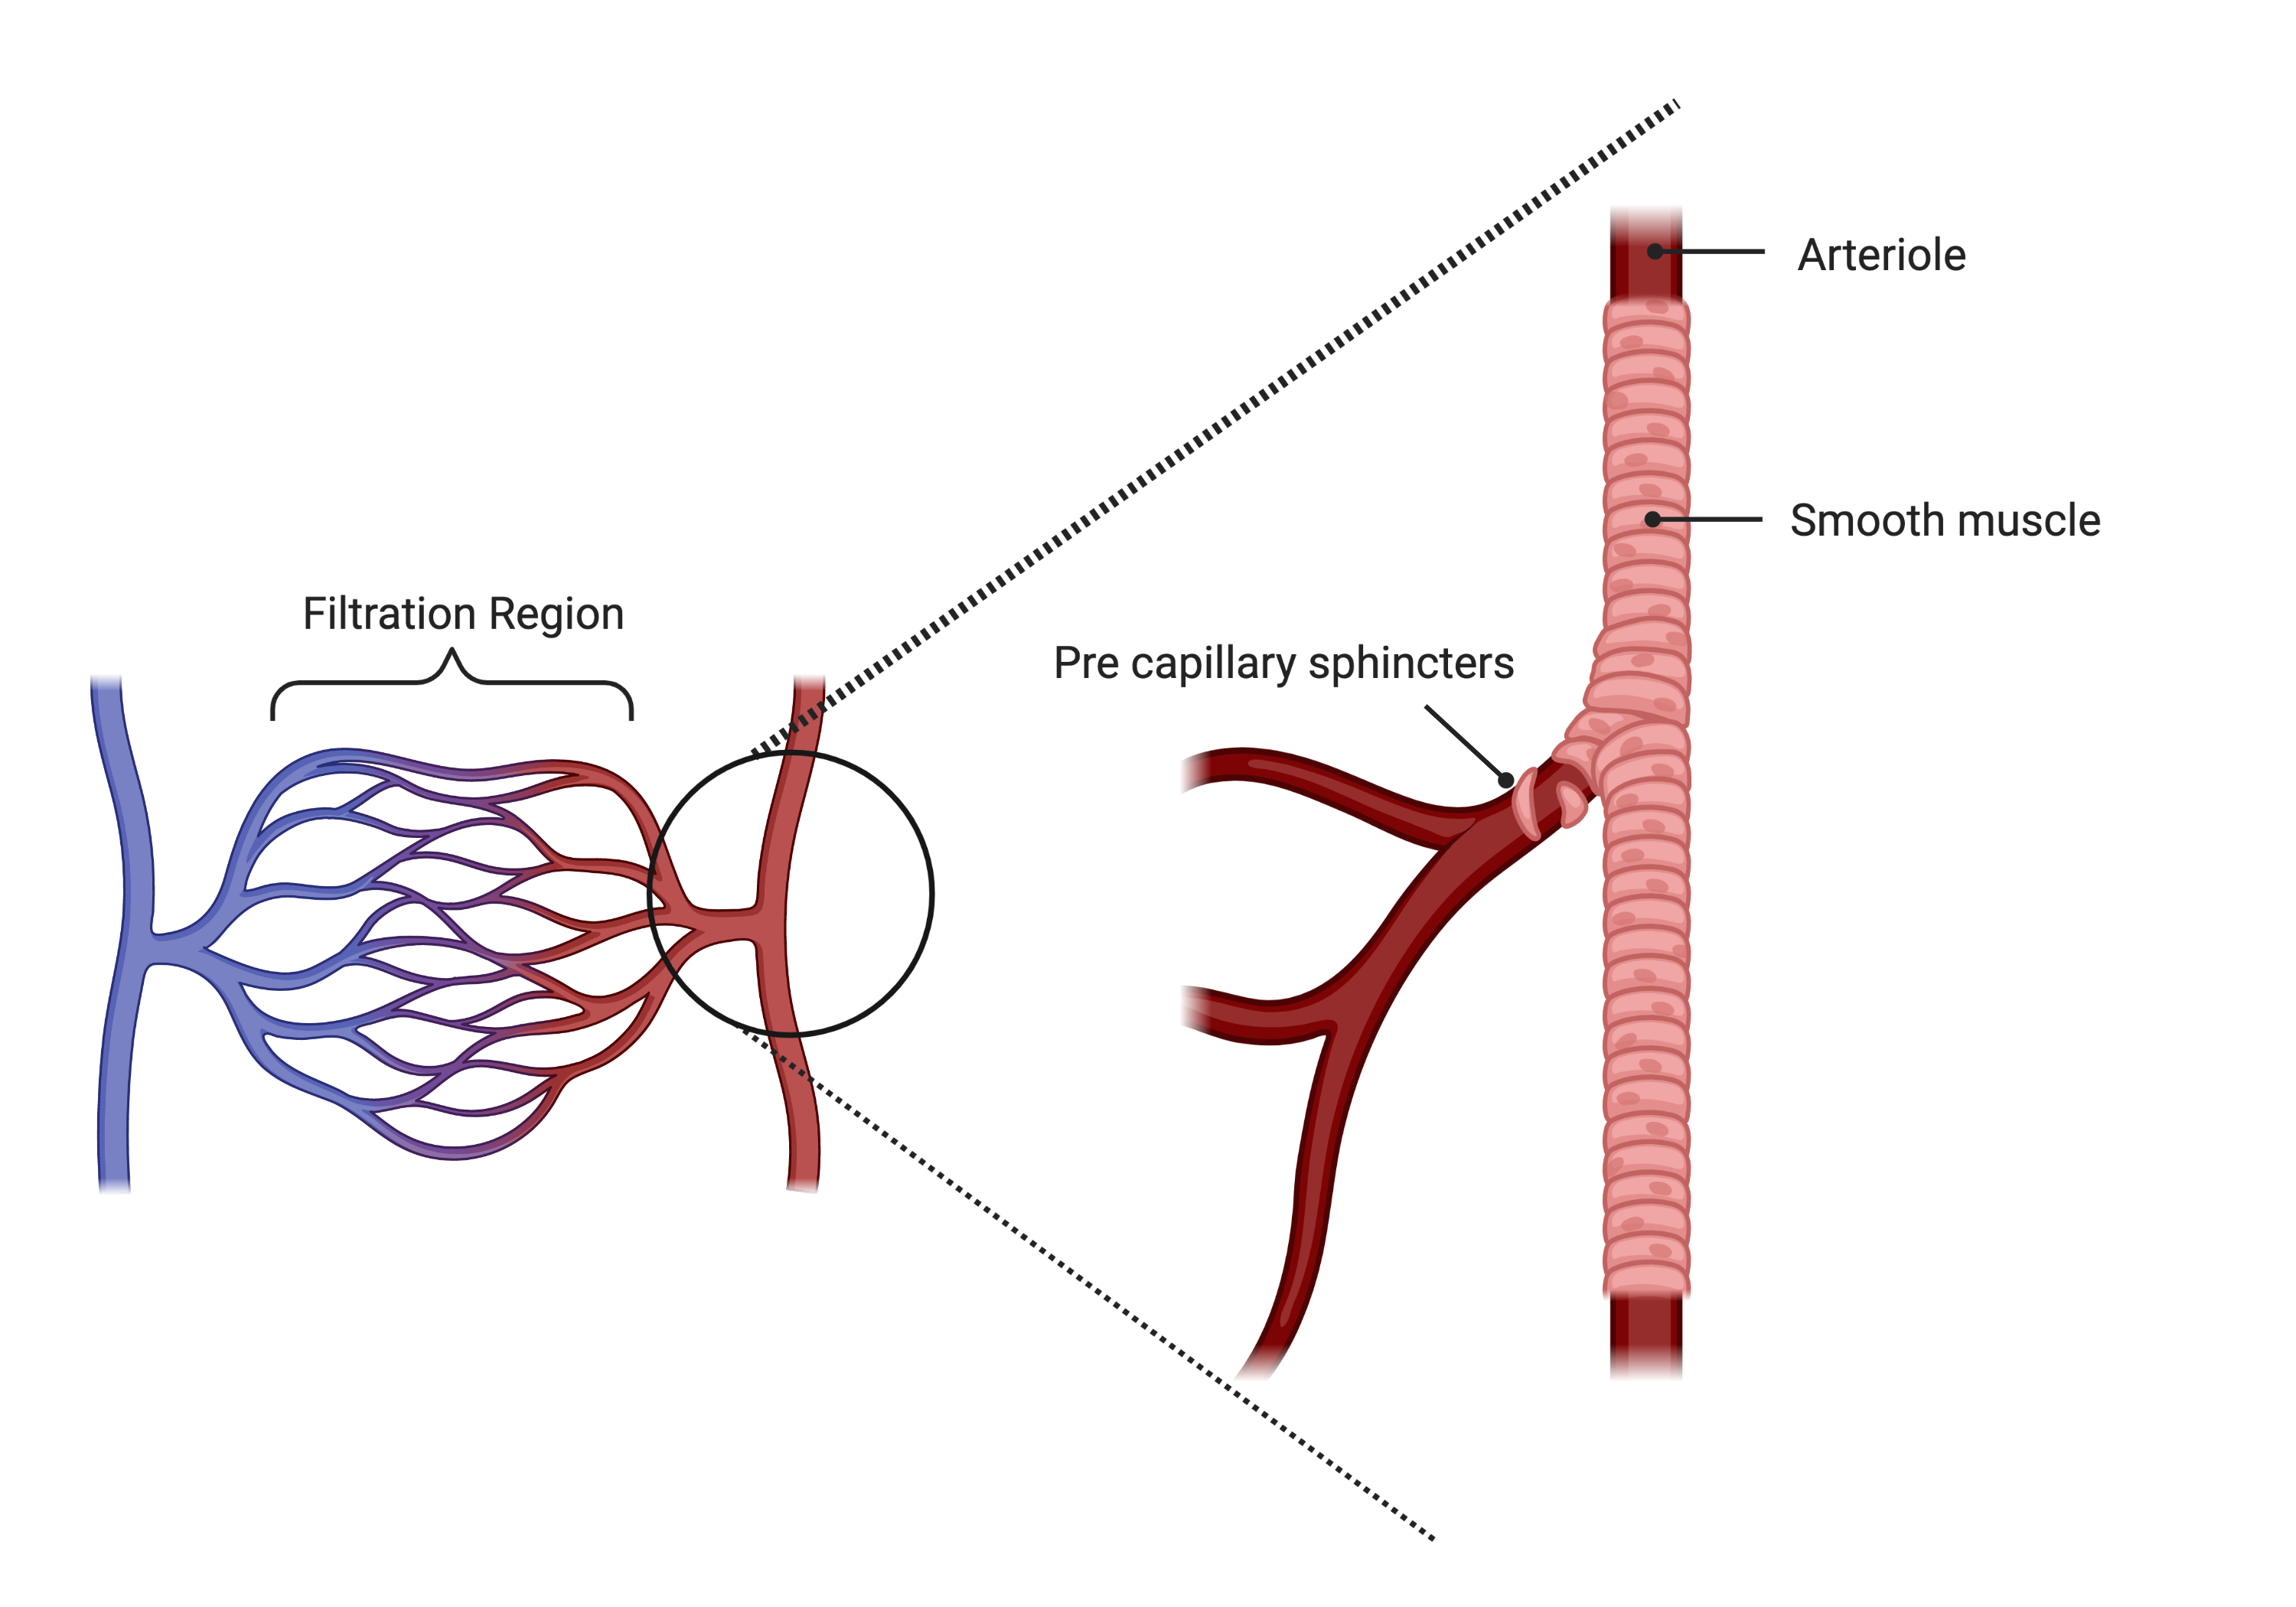
\includegraphics[width=0.7\linewidth]{./figure/capillaries.png}
    \caption{Capillary Anatomy \footnotesize{(Created with BioRender.com)}}
    \label{fig:capillaries}
\end{figure}

\paragraph{Capillary Dilation}
The capillary membrane can also undergo changes to the size of its openings which can allow cells that could not previously leave the vascular compartment to enter the interstitial fluid. When this occurs, such as with capillary dilation in response to cellular inflammatory mediators or other threats to the well being of cells, the white blood cells enter the interstitial space and change the osmolarity and osmotic pressure gradients. It is also possible that a high volume of blood in the capillaries, due to high pressure in the venuoles, will dilate capillaries. In this situation the high hydrostatic pressure tends to be more complicated by a low osmolarity as larger blood proteins of cells are able to leave the vascular compartment.

\subsection{Filtration Pressures}

Filtration is the normal process of exchanging vascular and interstitial fluid (and solute) for micro-circulation. When filtration does not work well there is either hypoxia due to ischemia (not enough $O_2$ being delivered due to no or limited capillary blood flow), extra cellular edema (excessive fluid in the interstitial space), or (rarely) increased blood volume from excessive fluid moving into the vascular space).

To promote normal filtration the overall filtration pressures (hydrostatic (P) and osmotic ($\pi$)) are slightly unbalanced. This unbalance tends toward pushing fluid and solute out of the vascular compartment and into the interstitial compartment, leaving some of the fluid and solute in the interstitial compartment. The volume of fluid and solute left in the interstitial compartment then enters the lymphatic system and reenters the vascular system after circulation and filtration through the lymph vessels and nodes. 

An equation that shows the relationship between the determinants for filtration is depicted in Figure \ref{fig:filtration_equation}. 

\begin{figure}[!h]
    \centering
    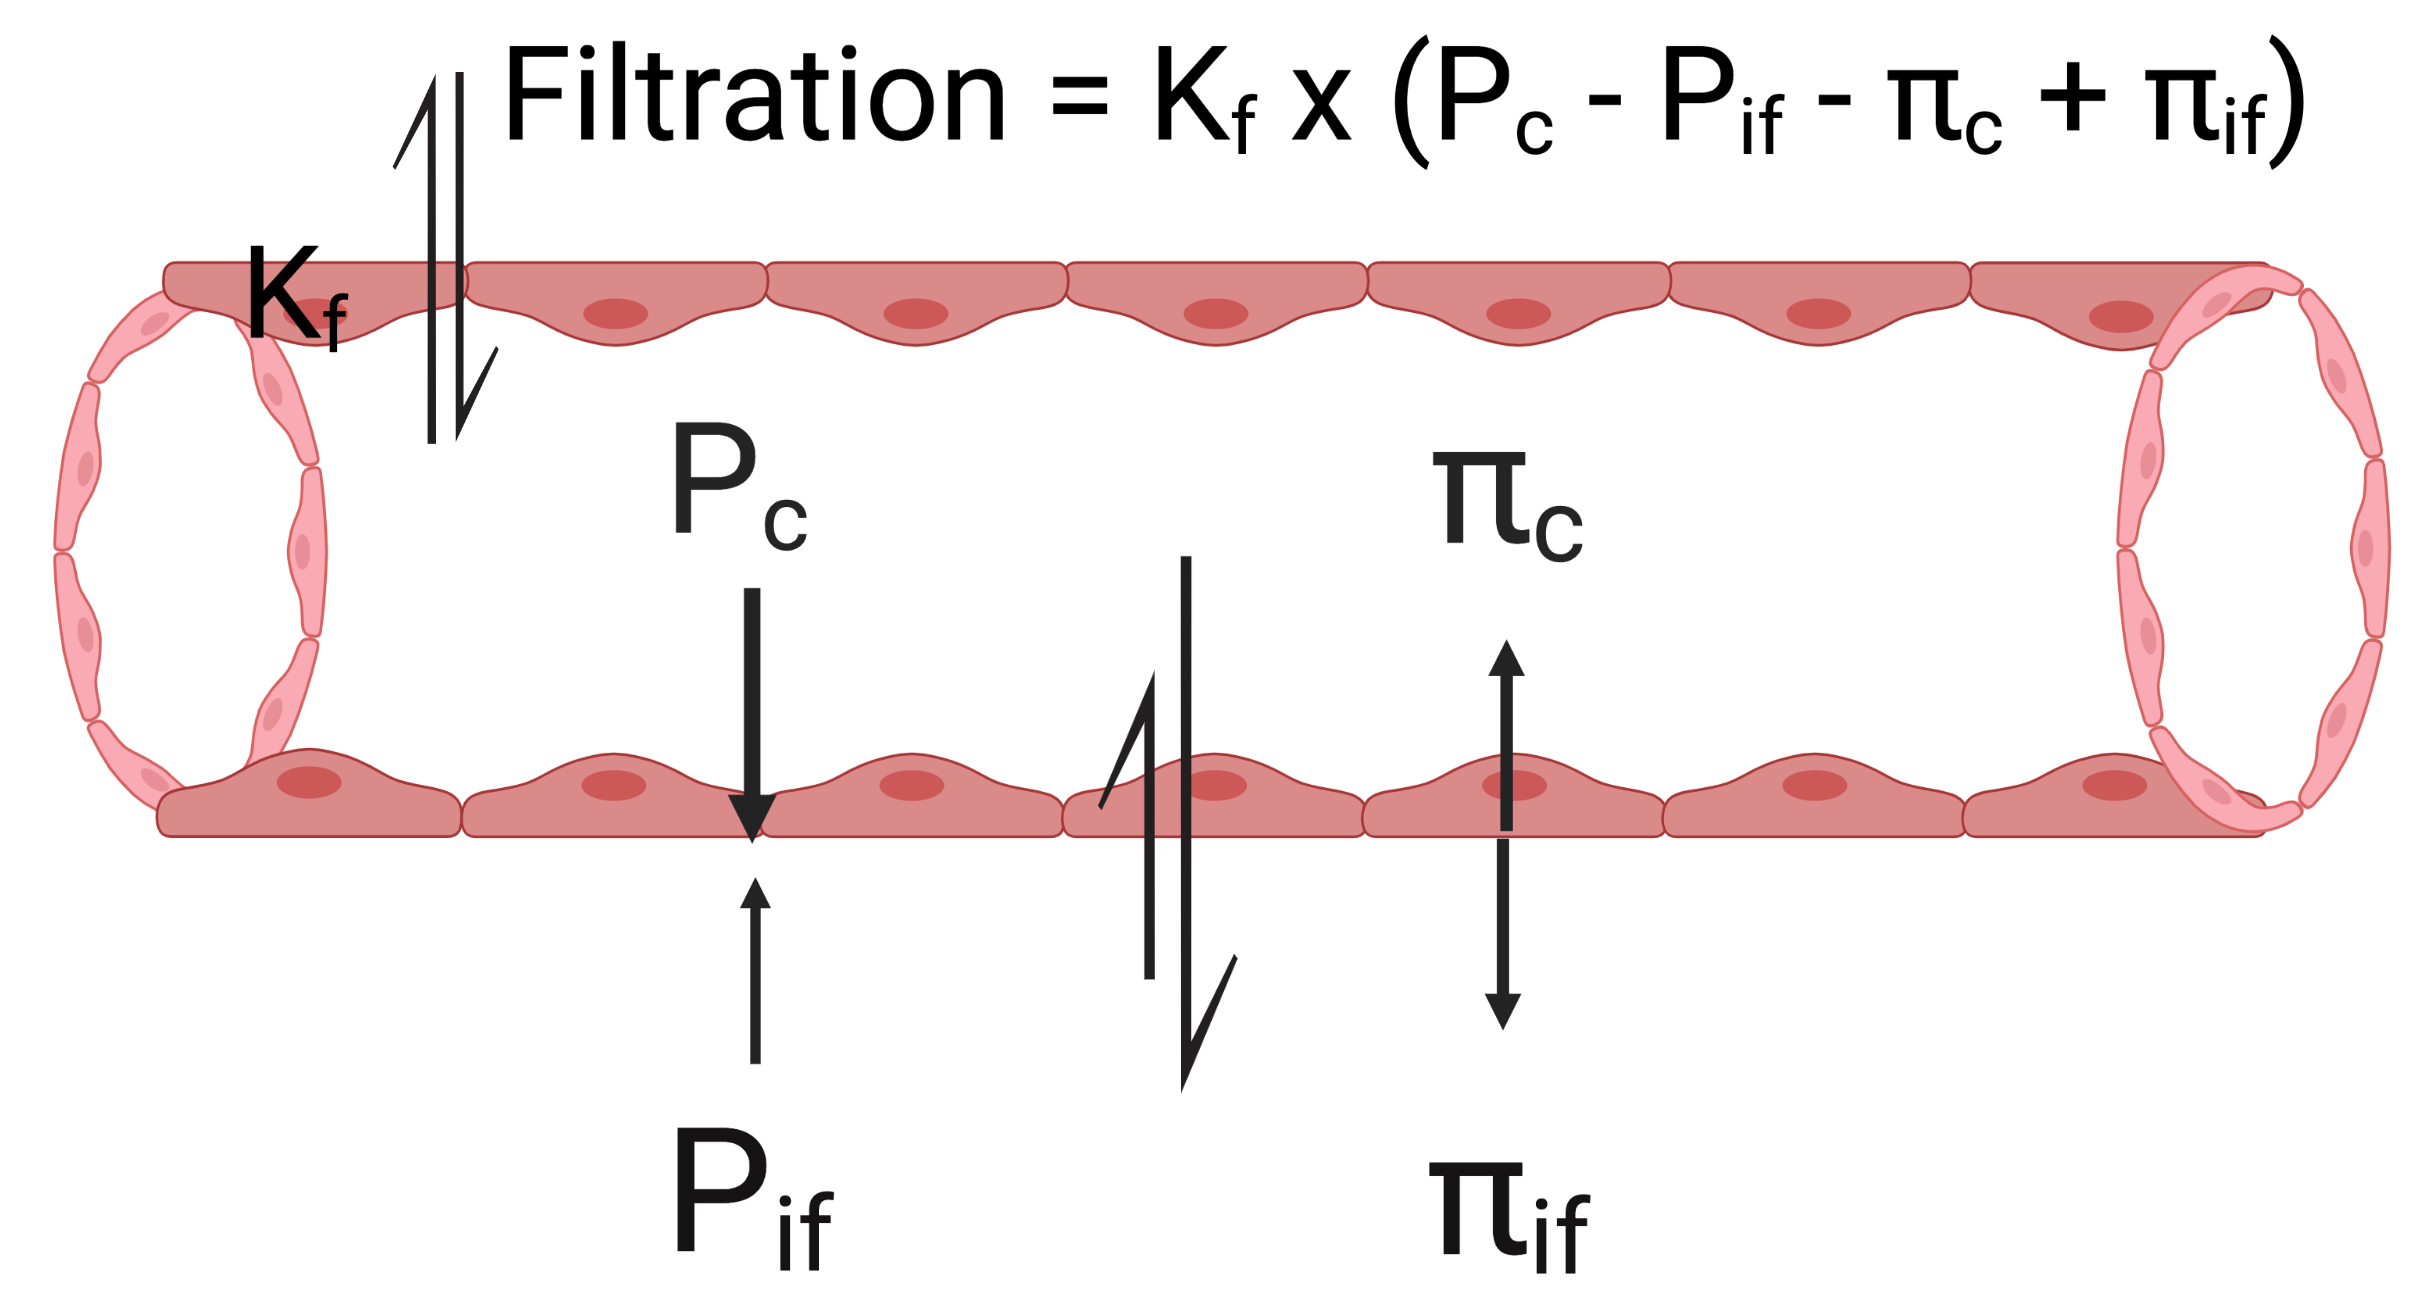
\includegraphics[width=0.7\linewidth]{./figure/filtration_equation.png}
    \caption{Filtration Equation \footnotesize{(Created with BioRender.com)}}
    \label{fig:filtration_equation}
\end{figure}

There are no constants in this equation, each parameter is a variable. The parameter $K_f$ is the filtration coefficient. 

$K_f$ is refers to the permeability of the capillary membrane. While not constant, it is relatively stable unless there are inflammatory mediators caused by injury or infection or very high capillary volumes that cause dilation. Dilation increases the $K_f$ by opening channels between endothelial cells of the capillary membrane. An increase in $K_f$ does not push or pull fluid into a particular compartment. It simply allows more fluid to be moved with any particular balance of filtration pressures.

$P_c$ refers to the hydrostatic pressure inside the capillary, and $P_{if}$ refers to the hydrostatic pressure inside the interstitial fluid (space). The hydrostatic pressures encourage flow from the compartment of higher pressure to lower pressure. $P_c$ pushes solute out of the capillary and into interstitial fluid when it is higher than $P_if$. $P_{if}$ pushes solute out of the interstitial fluid and into the capillary if it is higher than $P_c$.

$\pi_c$ is the osmolarity of the blood in the capillary. It exerts a pressure that pulls water into the capillary (from the interstitial fluid.  $\pi_{if}$ is the osmolarity of the interstitial fluid. It pulls water into the interstitial fluid (from the capillary). 

Since all four of these pressures work with or against one another the overall balance of these four pressures that determines filtration. 

If $(P_c - P_{if} - \pi_c + \pi_{if}) = 0$ there is no net change in vascular or interstitial volume and there would be no filtration. If $(P_c - P_{if} - \pi_c + \pi_{if}) > 0$ there is filtration with a net gain in the interstitial space. If $(P_c - P_{if} - \pi_c + \pi_{if}) < 0$ there is filtration and a net gain in the vascular space. Under normal circumstances, across the entire capillary, $(P_c - P_{if} - \pi_c + \pi_{if})$ is just slightly greater than 0 so that there is filtration and a net gain in the interstitial space that is picked up by the lymphatic system. 

\subsection{Micro-circulation Dynamics Through the Capillary}

The overall process of filtration is a bit more dynamic than depicted in Figure \ref{fig:filtration_equation}. The hydrostatic and osmotic pressures change as blood flows through the capillary, as depicted in Figure \ref{fig:Microcirculation_Regulation}. At the arterial end of the capillary (left side of the Figure) $P_c - \pi_c - P_{if} + \pi_{if} > 0$ which drives solute out of the capillary into the interstitial space. Since the larger items in the blood such as cells and proteins do not move into the interstitial space the $\pi_c$ of the capillary blood increases as the fluid that leaves has a lower osmolarity. Also, as the capillary blood loses volume the the $P_c$ drops. The movement of fluid from the blood into the interstitial space lowers the $\pi_{if}$ and raises the $P_{if}$.

\begin{figure}[!h]
    \centering
    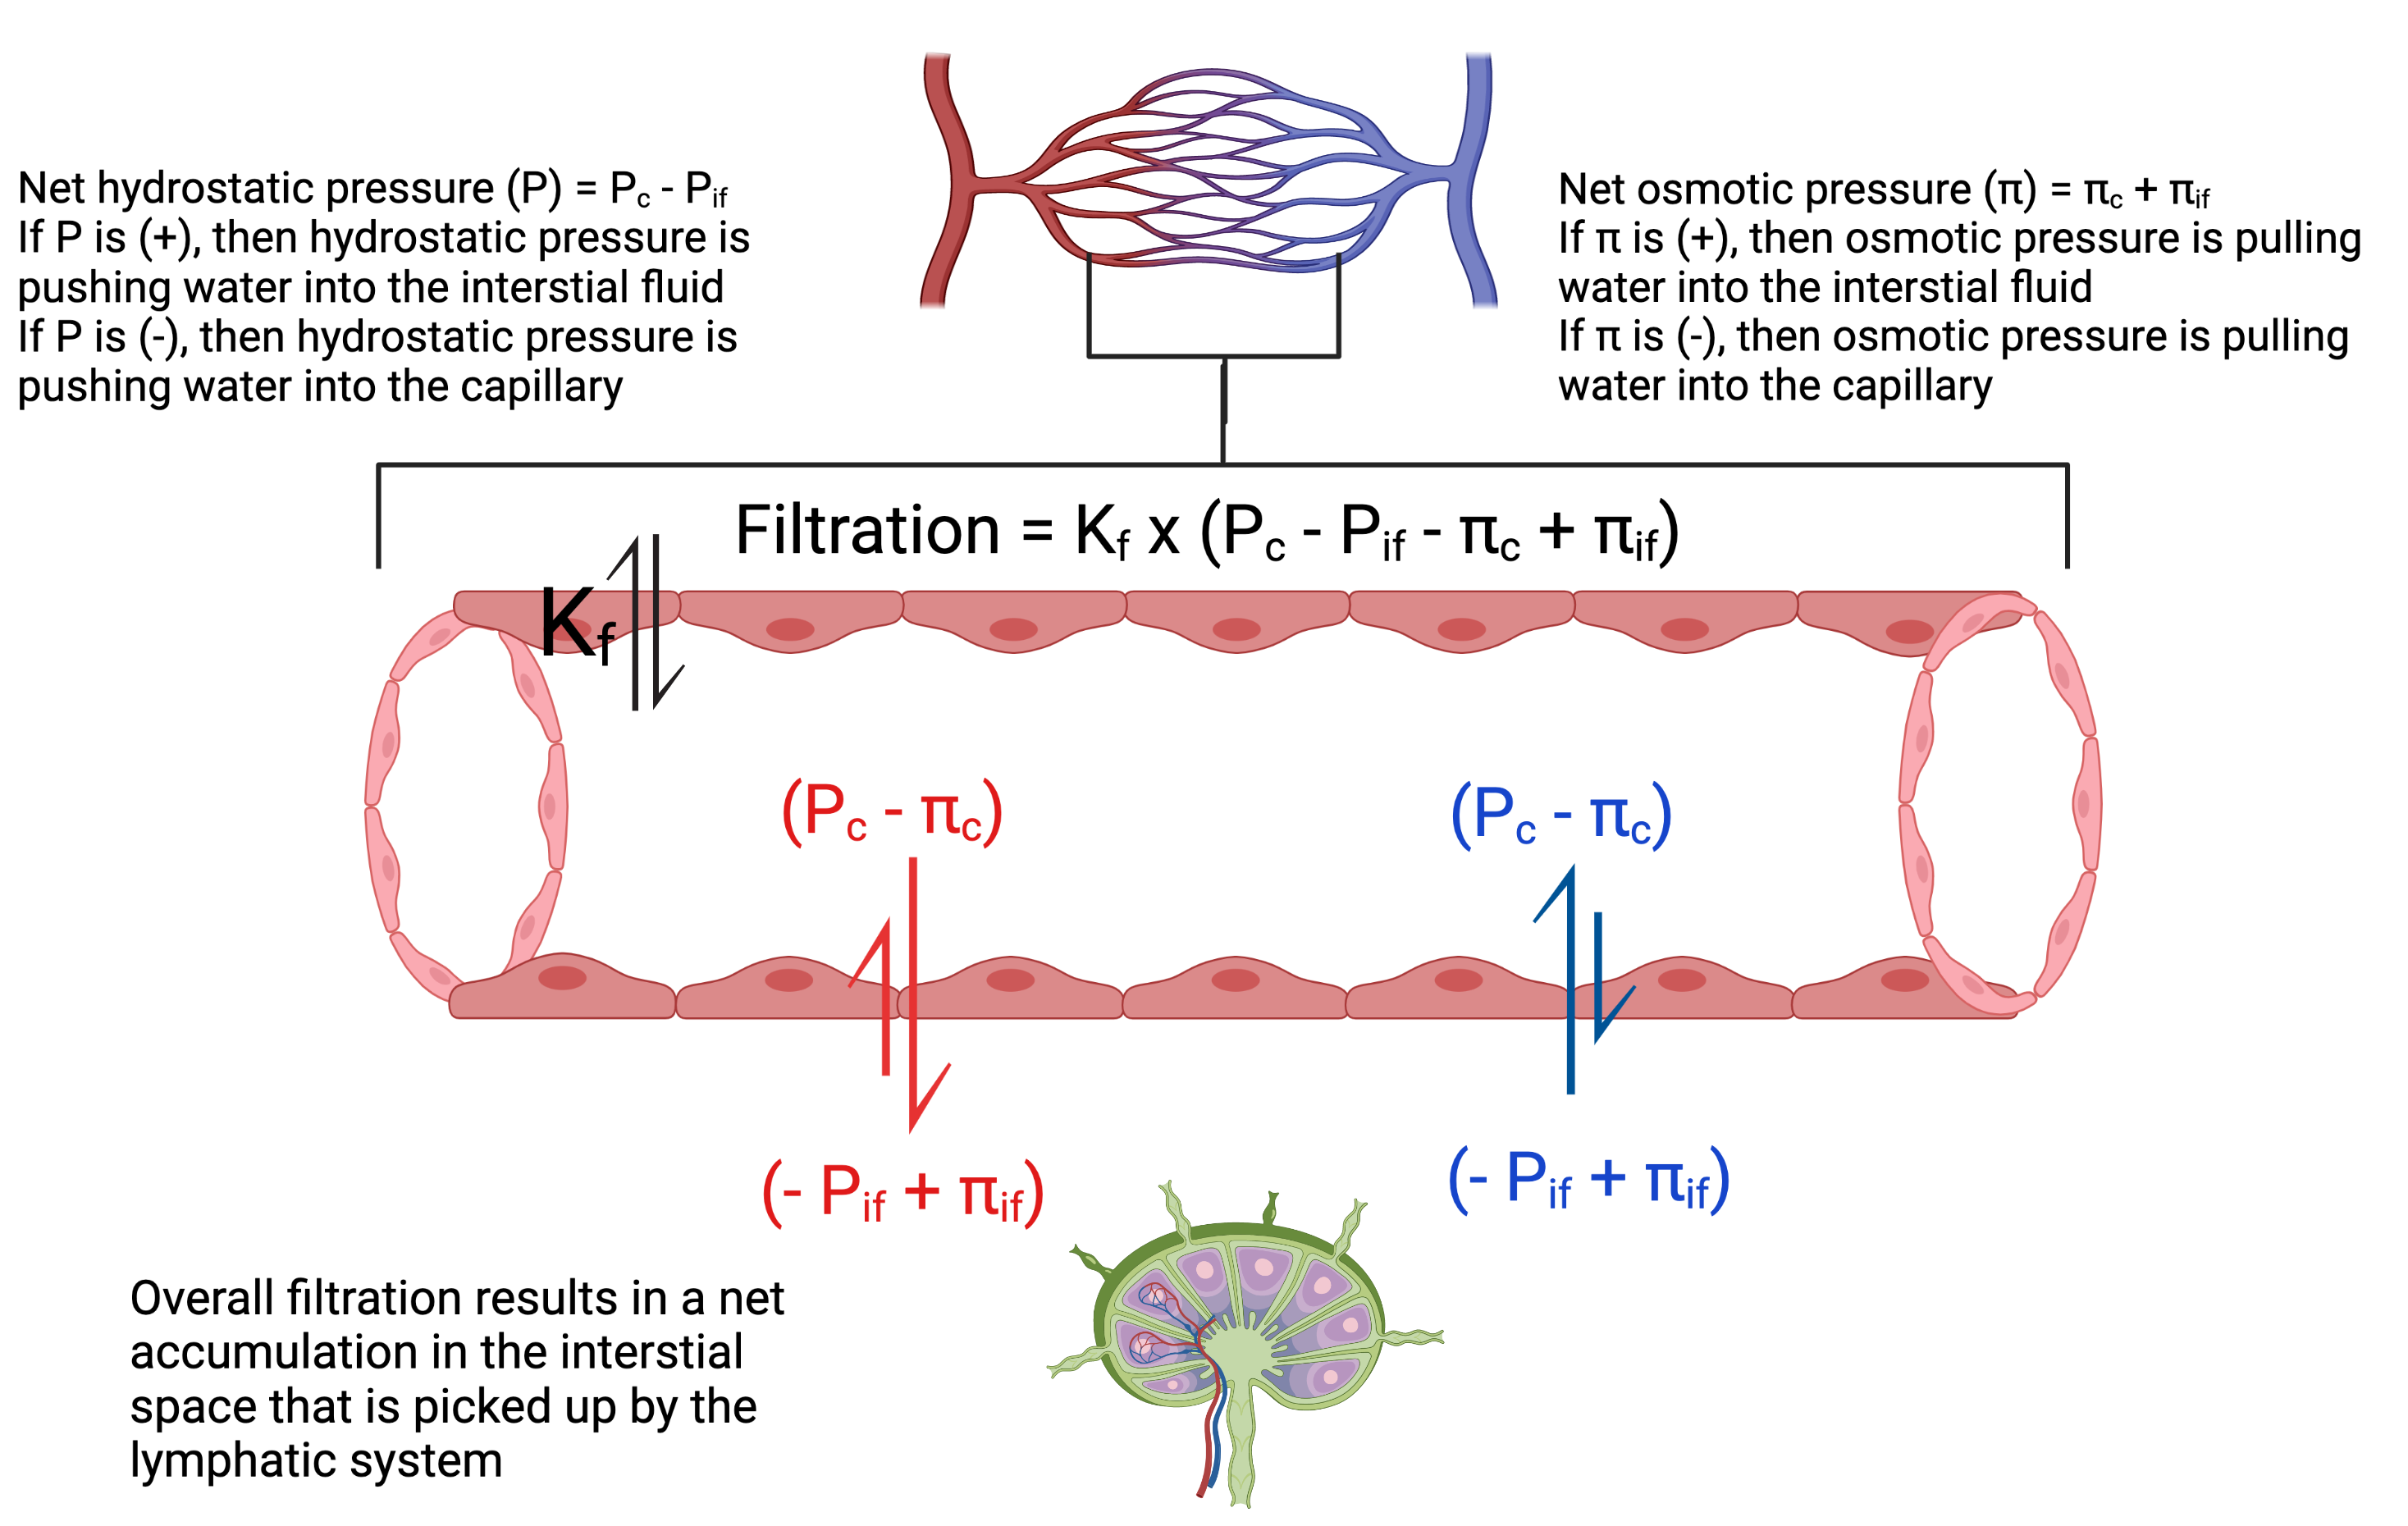
\includegraphics[width=1\linewidth]{./figure/Microcirculation_Regulation.png}
    \caption{Regulation of Micro-Circulation \footnotesize{Created with BioRender.com}}
    \label{fig:Microcirculation_Regulation}
\end{figure}

The overall effect of these changes means that on the venous end of the capillary $P_c - \pi_c - P_{if} + \pi_{if} < 0$ which pulls fluid back into the capillary.  The filtration on the arterial end (fluid pushed out of the capillary) is greater than the filtration on the venous end (fluid pulled into the capillary) so that there is a net positive filtration. This means some of the capillary fluid stays in the interstitial fluid and is picked up the lymphatic system. This more detailed picture of what is happening accounts for the dynamic filtration process going on in capillaries throughout the body. When the fluid on the arterial end of the capillary is pushed out it mixes with interstitial fluid. Then approximately 80\% of fluid is pulled back into the capillary on the venous end. The end result is substantial overall mixing of vascular and interstitial ECF ensuring continuity of ECF throughout the body for homeostasis of ions, delivering nutrients, and removing waste. Additionally, since the remaining 20\% enters the lymphatic system there is a screening process on the plasma passing through the lymphatics which has significant immunological benefits.

\subsection{Factors that Prevent Extra Cellular Edema}

There are a number of situations that result in changes to the overall filtration balance and result in interstitial edema. Some of these situations are minor and self limiting. Mild edema in the lower extremities after a day of being upright (mostly standing) is due to elevated venous pressures increasing $P_c$. There are two safety factors that prevent such situations from becoming severe edema (See Figure \ref{fig:Factors_Prevent_Edema}). First, low tissue compliance limits the hydrostatic pressure gradient as more fluid accumulates in the interstitial space (low compliance means higher pressure with a small change in volume, an increased $P_{if}$). Second, as edema develops there is a decrease in $\pi_{if}$. Third, lymphatic flow can increase by as much as 50-fold. These three factors also interact. As lymphatic flow increases the decrease in interstitial fluid protein further decreases the $\pi_{if}$ concentration in the interstitial fluid reduces the osmotic pressure.

\begin{figure}[!h]
    \centering
    \includegraphics[width=1\linewidth]{./figure/Factors_Prevent_Edema.png}
    \caption{Factors that Prevent Edema \footnotesize{Created with BioRender.com}}
    \label{fig:Factors_Prevent_Edema}
\end{figure}

\subsection{Extra Cellular Edema}

There are two general causes of extracellular edema. First, a higher overall filtration pressure (>> 0) with a greater net flow of solute from the capillary to the interstitial fluid that is not returned to the capillary. This can be caused by anything that increases capillary permeability ($K_f$), alters hydrostatic pressure, or alters osmotic pressure. In these situations the increase in filtration exceeds the capacity of a normal lymphatic system. The problem is caused not by faulty lymphatics, but by an increase in filtration.
The second general cause of extra cellular edema is failure of the lymphatics to pick up extra fluid from the interstitial fluid. In this situation filtration is normal, but the lymphatics are not able to pick up the 20\% of fluid that normal filtration does not return to the capillary. There is a faulty lymphatic system, the edema caused by this situation is called lymphedema.

\begin{figure}[!h]
    \centering
    \includegraphics[width=1\linewidth]{./figure/Extracellular_Edema.png}
    \caption{Extra Cellular Edema \footnotesize{Created with BioRender.com}}
    \label{fig:Extracellular_Edema}
\end{figure}

Three particular situations are presented in Figure \ref{fig:Extracellular_Edema} that can cause interstitial edema. Please note that these are not mutually exclusive. 
In situation 1 inflammatory mediators (local damage) or a cytokine storm (systemic inflammation) results in increased $K_f$ which results in a much higher than normal filtration. Since a high $K_f$ can also include movement of larger molecules from the capillaries into the interstitial fluid such as proteins and white blood cells they can have a secondary effect of increasing the $\pi_{if}$ which contributes to the edema. 
In situation 2 there are two examples. To the left, heart failure increases venous pressure due to impaired flow through the heart. The increase in venous pressure increases $P_c$ which pushes more solute out of the capillaries. If this delay in flow is on the left side of heart the edema occurs in the lungs. If it is on the right side of the heart the edema occurs in the extremities (primarily the lower extremities since it is made worse by gravity). It is important to note that the most common cause of a heart pump problem on the right side of the heart is a problem with the left side heart pump. The second example for situation 2 is a reduction in albumin production in liver disease (such as cirrhosis). The reduction in the blood protein albumin reduces $\pi_c$ which lowers the pull of fluid back into the capillaries.
In situation 3 there is failure of the lymphatic flow combined with a lower $P_if$ due to an increase in the compliance of the interstitial space. Without lymphatics removing solute from the interstitial fluid there is also an increase in $\pi_{if}$ despite an increase in fluid.
As with any set of possible comorbidities that are not mutually exclusive (which is most of them), the worst case scenario includes combinations of situations. For example, someone with heart failure and liver disease getting COVID and having a systemic cytokine storm and local inflammatory mediators associated with local hypoxia. 

\section{\textit{Muscle Connections}}

\subsection{Smooth Muscle}

Smooth muscle is present in the walls of organs (i.e. stomach, intestines), passageways (arteries, veins, bronchioles). They are spindle shaped and much shorter than skeletal muscle fibers. Smooth muscles do not have striations but they do have actin and myosin. Unlike skeletal muscles the actin and myosin is not so precisely arranged to form sarcomeres. Fiber arrangement is highly variable between smooth muscles and dependent on the role. 

\paragraph{Smooth Muscle Activation}

Unlike skeletal muscle the tension of smooth muscle fibers acts on other smooth muscle fibers for the purpose of making a compartment or passageway narrow (such as vasoconstriction or vasodilation). Actin is anchored by dense bodies (similar to the Z-discs) which are fastened to the sarcolemma. A smooth muscle contraction is activated by calcium which is supplied by the SR and directly from the  extracellular fluid moving through channels in the smooth muscle sarcolemma. Calcium binds to calmodulin (smooth muscle version of troponin-tropomyosin). When activated the sliding filament theory is similar to skeletal muscle, and the overall effect is tension that attempts, and in most cases does, shorten the fiber. Shortening occurs in most cases because the tension developed does not usually have high resistance preventing the shortening, or at least there are far less variations in the resistances that smooth muscles must compete with (other than perhaps the uterus during labor and delivery where contractions are pushing against a substantial resistance). Since smooth muscle is attached to dense bodies that are attached to the sarcolemma, in addition to shortening smooth muscle tends to also pull inward from all around itself. 

\paragraph{Smooth Muscle Excitation}

Smooth muscle excitation is initiated by the influx of $Ca^{2+}$ which depolarizes the membrane, activates crossbridges and excites SR to release additional $Ca^{2+}$. The wave of excitation over the sarcolemma from fiber to fiber because unlike skeletal muscle when one smooth muscle fiber is activated all should be activated (single-unit organization).

\paragraph{Smooth Muscle Regulation}

Smooth muscles can be organized as a single-unit (more common) or as as a multi-unit.
Single unit smooth muscles have gap junctions that allow quick sharing of $Ca^{2+}$ between cells during excitation so that all the fibers are activated together as a single-unit. Single-unit smooth muscle surrounds the visceral organs and the small blood vessels. Single-unit smooth muscle is regulated by both the autonomic nervous system and stretch. The autonomic nervous system (sympathetic nerves and hormones, parasympathetic nerves) can excite single unit smooth muscles for more or less tension using frequency summation (but not motor unit summation because there are no motor units). Autonomic nerve excitation of single-unit smooth muscle does not occur at precisely located motor end plates and neuromuscular junctions. Instead the autonomic nerves have locations along the nerve fibers called varicosities that are filled with with vesicles that release a neurotransmitter that is then free to bind to any acceptable and available smooth muscle receptor (See Figure \ref{fig:Smooth_Muscle}). Single-unit smooth muscle also can be excited by stretch in what could be considered a local stretch reflex. Unlike a muscle spindle stretch reflex in skeletal muscle that loops through the spinal cord, the smooth muscle stretch reflex occurs because the mechanical stretch of the fiber opens $Ca^{2+}$ channels that both excite and activate the smooth muscle.

\begin{figure}[!h]
    \centering
    \includegraphics[width=0.5\linewidth]{./figure/Smooth_Muscle.jpg}
    \caption{Smooth Muscle \footnotesize{CCBY4.0 from Version 8.25 from the Textbook OpenStax Anatomy and Physiology}}
    \label{fig:Smooth_Muscle}
\end{figure}

Multi-unit smooth muscle fibers can be regulated by both frequency and fiber unit based excitation. To allow this increase in precision of tension for multi-unit smooth muscles they have precision between the autonomic nerves and the smooth muscle fibers. They also do not have gap junctions so excitation does not spread from one fiber to the next. Like skeletal muscle, excitation is confined to the fiber that was originally excited. Excitation for multi-unit smooth muscles also does not originate from stretching. The large blood vessels and the respiratory airways have multi-unit smooth muscle.

\paragraph{Smooth Muscle Tone}

Activation continues until ATP-dependent calcium pumps actively transport $Ca^{2+}$  ions back into the SR and out of the cell. Many smooth muscles maintain a low concentration of  $Ca^{2+}$ to maintain tone. In the case of blood vessels this is important because if all blood vessels were fully dilated (no smooth muscle tone) then blood pressure would drop so low that maintaining upright posture would not be possible. Abnormalities in the smooth muscle tone of blood vessels one possible cause for conditions such as orthostatic hypotension, postural orthostatic tachycardia syndrome (POTS) and vasovagal syncope.

To allow smooth muscles to maintain tone for prolonged periods without rest they can maintain contractions even as  $Ca^{2+}$ is removed and myosin is inactivated. This can happen due to a subset of crossbridges form latch-bridges. Latch bridges keep actin and myosin connected without ATP, allowing tension (as tone) in smooth muscle that lines arterioles and other visceral organs with very little energy expenditure.

\subsection{Compression}

Compression is an important part of edema management (RICE stands for rest, ice, compression and elevation). Elevation reduces hydrostatic pressure. Compression increases the gradient between venous pressure being compressed and venous pressure further away from compression (usually more proximal). This encourages reduction in $P_c$ which allows more fluid to reenter the capillary during filtration. The pressure also increases the pressure gradient between the local lymphatics and the lymph vessels not being compressed which facilitates movement of edema also into the lymphatics.

Compression has also now become more common for recovery to increase micro circulation to remove post exertion waste and delivery needed nutrients. It works through the same mechanisms as above, but in response to small amounts of local edema from a combination of increased cellular and interstitial osmolarity, and increased cellular and capillary permeability ($K_f$). The compression does not alter the permeability, or the osmolarity changes, but it does reduce $P_c$ which shifts the balance of the filtration equation to encourage movement of edema from the area and into both the capillary and lymphatics.

Compression is also gaining popularity during endurance events, particularly running. However whether there is a benefit and what the mechanisms are remains elusive \cite{mota_effects_2020}. There are several factors to consider with compression during endurance events and it goes beyond what can be discussed in this already long chapter. On reason proposed for compression during an endurance event is to maintain vascular volume. With such long events may be difficult to maintain complete hydration. However, a small amount of dehydration increases $\pi_c$ which facilitates return of fluid into the circulation. There is also a strong muscle pump working to maintain venous flood flow, once again, facilitating return of fluid to the capillary (keeps $P_c$ low due to venous blood flow and would also promote lymphatic blood flow). So it is unclear whether sustaining vascular volume makes mechanistic sense. It's possible that it facilitates greater overall micro circulation and filtration which encourages greater nutrient delivery and waste product removal from the lower extremities. It is also quite possible that whether compression with endurance running provides a benefit is highly contextual (i.e. related to many interacting causal factors, complex) and is difficult to completely account for in research studies. In such situations it may be best trialed by individuals with self experimentation, which requires a slight reconsideration of what it means to gather evidence \cite{anjum2020rethinking}.

\section{Summary}

The ECF supports muscle fibers by having and providing resources for muscle function. ECF requires micro-circulation. Micro-circulation between cells and the ECF requires balanced osmolarity and a functioning semi-permeable sarcolemma (cell membrane). Micro-circulation between the compartments of ECF, vascular (capillary) and interstitial spaces (fluids) requires filtration. Filtration requires a small unbalance of hydrostatic and osmotic pressures between the capillaries and the interstitial spaces as well as a semi-permeable capillary membrane. Water, ions, molecules and nutrients are constantly circulating between the vascular (capillaries and lymphatics) and interstitial compartments of the ECF. 
The amount of blood flowing through capillaries can be varied by local and neuroendocrine factors by altering the degree of vasodilation and vasconstriction of arterioles, pre-capillary sphincters and venuoles. Vasoconstriction occurs through tone (sustained contraction) of smooth muscles. 
All causes of intra cellular and extra cellular can ultimately be broken down into altered membrane permeability (cell or capillary), imbalances of osmolarity (and osmotic pressure), imbalances of hydrostatic pressure, and lymphatic function. Compression is an effective intervention for edema due to its facilitation of venous blood flow which reduces $P_c$.


\section{Next Steps}

The next chapter is on blood flow (circulation), the flow of blood through the entire circulatory system. Circulation of blood through the entire body ensures regular mixing of the ECF contents throughout the body. This mixing ensures consistency of ECF contents and a stable environment for all the cells of the body. Circulation allows each supporting system to contribute by either to adding to ECF or removing by-products from ECF. Circulation also allows supporting systems to communicate with each other based on the circulating substances and messages (hormones). Blood flow requires a pump (the heart), vessels from the heart to the capillaries (arteries) and from the capillaries back to the heart.

\printbibliography[heading=subbibintoc]

% !TEX root = ../notes_template.tex
\chapter{Circulation}\label{chp:blood_flow}
Updated on \today
\minitoc
This chapter covers the blood flow support of micro-circulation, which supports the ECF, which supports skeletal muscle function. Blood flow includes the heart as a muscular pump (cardiac function) and the two vascular circuits that the pump circulates blood through (systemic and pulmonary circulation). All together these components can be referred to as the cardiovascular system (anatomical perspective) or circulation (physiological perspective). 

The supportive role of circulation is reliant on cardiac muscle. The relationship between circulation and cardiac muscle is similar to the relationship between movement and skeletal muscle. Concepts from skeletal muscle such as tension, excitation, regulation and energetics are applicable to cardiac muscle and are included. It is useful to compare and contrast cardiac muscle with skeletal muscle across these concepts while focusing on how the differences enable the act of circulation. However, this is not an attempt to shift the focus from a skeletal muscle approach to a cardiac muscle approach. The primary goal of this chapter is an understanding of circulation in its supportive role for skeletal muscle. Therefore, there is less emphasis on the details cardiac muscle and more emphasis on the act of circulation.\footnotemark\footnotetext{Unlike in Part I where there was more emphasis on the details of skeletal muscle and less emphasis on the various manifestations of the act of movement.} Emphasis on circulation means cardiac skeletal muscle is discussed in support of circulation. This is realized most in the section on regulation which discusses regulation of cardiac muscle as one aspect of the regulation of circulation along with other aspects of the regulation of circulation.

Blood flow is critical for sustaining the micro-circulation of the ECF for cellular functions throughout the body. Without circulation cells with a high resting metabolism such as the brain and heart can only survive for minutes. The lack of $O_2$ delivery, and lack of $CO_2$ removal being the first two problems that threaten cell life. Problems with blood flow can limit the metabolic function of muscles. With a fully supportive circulation the skeletal muscles can generate a wide range of tension in support of movement. The support of movement requires attaining and sustaining tension. Attaining and sustaining tension requires energetics, which requires circulation. Limitations in circulation limit attaining, and perhaps more noticeably, sustaining tension, which both limit function.  

The importance of circulation for life and function makes it a highly studied area of physiology. Since it has been highly studied it has several useful models for understanding circulation. After reviewing the important structures for blood flow the chapter introduces several of the useful models (in the form of equations that demonstrate relationships).


\vspace{5mm}

\textbf{Objectives include:}
\begin{enumerate}
    \item Describe how the anatomy of the heart and blood vessels supports circulation. 
    \item Identify cardiac anatomy structures.
    \item Explain and Interpret models (equations) of cardiac output, blood pressure and resistance.
    \item Apply equations of cardiac output, blood pressure and resistance (including Poiseuille's Law) to explain and evaluate the function and possible dysfunction of circulation.
    \item Explain blood flow regulation based on BP regulation including the baro-receptors and other reflexes.
    \item Interpret the events of vasovagal syncope.
    \item Explain the response of blood pressure to a graded exercise test.
    \item Compare and contrast cardiac and skeletal muscle based on tension, excitation, regulation and energetics.
    \item Explain factors that influence cardiac output (including preload, afterload, intropy, chronotropy).
    \item Explain the relationship between RPP and myocardial oxygen demand.
    \item Explain how the unique characteristics of cardiac muscle tension, excitation (automaticity, rhymicity, conductivity, contractility), regulation and energetics support blood flow.
    \item Explain the cardiac cycle (to the point of drawing and explaining all aspects of Wiggers Diagram).
    \item Explain systemic circulation including its distribution and cardiac index; cardiac circulation and pulmonary circulation.
    \item Perform an ECG rhythm analysis including the identification of arrhythmias and myocardial blood flow abnormalities.
    \item Perform and interpret cardiovascular tests and measures including: Heart rate and Blood pressure
\end{enumerate}

\section{Structures of Blood Flow}

The heart and the roots of the great vessels occupy the pericardium, which is located in the mediastinum. The sternum, the costal cartilages, and the medial ends of the third to fifth ribs on the left side of the thorax create the anterior border of the mediastinum. It is bordered inferiorly by the diaphragm, posteriorly by the vertebral column and ribs, and laterally by the pleural cavity (contains lungs). Specific cardiac structures and vessels are depicted in Figure \ref{fig:Cardiac_Anatomy}.

\begin{figure}[!h]
    \centering
    \includegraphics[width=1\linewidth]{./figure/Cardiac_Anatomy.png}
    \caption{Cardiac Anatomy \footnotesize{(Created with BioRender.com)}}
    \label{fig:Cardiac_Anatomy}
\end{figure}

Beyond being familiar with the structure in Figure \ref{fig:Cardiac_Anatomy} that are utilized throughout the chapter, there are several important structural takeaways.

\begin{itemize}
    \item Structurally there are four chambers, right and left atria (RA and LA); right and left ventricle (RV and LV) (the anatomical view).
    \item The four chambers form two primer-pumps for two circulations (right and left), RA and RV for the pulmonary circulation; and LA and LV for the systemic circulation (which includes all skeletal muscles and the heart itself) (the pump view).
    \item Cardiac muscle (myocardium) is thicker in the ventricles than the atria; and on the left side than the right side.
    \item The four chambers are divided into two excitation regions, RA and LA for atrial excitation; and RV and LV for ventricular excitation (the excitation view).
    \item The amount of tension and excitation is related to the thickness of the myocardium; which is based on how much pressure that chamber must generate for blood flow.
    \item Blood flow between the right and left primer-pumps is prevented by a septum (septal wall), also myocardium, that is thinner than the outer myocardial wall; and also thicker in the ventricles than the atria.
    \item Blood flow direction is guided by four one-way valves. Blood flow occurs due to pressure gradients - there is nothing inherently directional about pressure gradients other than high pressure to low pressure - therefore the valves are necessary to keep blood flowing from a chamber to the next chamber and now "backwards".
    \item All blood flow from the gut and lower extremity passes through the descending aorta; and comes to the heart through the inferior vena cava.
    \item All blood flow from the upper extremities and head passes through the great vessels (first three branches off of the aorta); and comes to the heart from the superior vena cava.
    \item For blood to flow through the circulation, venous pressure must be lower than arterial pressure
    \item Venous pressure (systemic in the RA; pulmonary in the LA) refers to the pressure that is the final end point for all venous blood flow returning to the heart which must, for blood flow to occur, have the lowest venous blood pressure of the respective circulations ($P_{RA} = 0$ when the RA is not generating tension). \item Ventricular systolic pressure refers to the pressure in the ventricles during active tensioning (contraction), for blood flow to occur it must have the highest arterial pressure of the respective circulations. The right sided ventricular systolic pressure is lower than the left sided ventricular systolic pressure, the respective circulations are considered low and high pressure.
    \item Because the ventricular systolic pressures must be the highest through the circulation, the tricuspid valve (between the RA and RV) and the bicuspid (mitral) valve (between the LA and LV) have additional support supplied by the papillary muscles and chordae tendonae (the support does not help them open, it prevents them from allowing backflow while closed).
    \item Because the LV has greater pressure than the RR, the mitral valve papillary muscle and chordae tendonae are more developed
    \item The aortic valve, which is not supported by papillary muscle, is under more pressure than the tricuspid valve because the aortic pressure is the second highest pressure in the circulation, however aortic peak pressure is short lived because of how rapidly blood flows out of the aorta.
\end{itemize}

\section{Blood Flow}

\subsection{Cardiac Output}

Blood flow (circulation) is measured and assessed based on the cardiac output ($\dot{Q}$) in liters (or mL) per minute. $\dot{Q}$ is directly proportional to the overall pressure gradient and inversely proportional to resistance to circulation:

\begin{equation}
    \dot{Q} = \frac{P_{a} - P_{RA}}{TPR}
    \label{Q}
\end{equation}

Where $P_{a}$ is pressure in the arteries (highest in the aorta); $P_{RA}$ is central venous pressure in the RA; and $TPR$ is the total peripheral resistance.

Since $P_{RA}$ normally approximates 0, the equation can be simplified to:

\begin{equation}
    \dot{Q} = \frac{P_{a}}{TPR}
    \label{Q_simplified}
\end{equation}

Another equation that is utilized to conceptualize $\dot{Q}$ is:

\begin{equation}
    \dot{Q} = HR \times SV
    \label{Q_HRSV}
\end{equation}

where HR is heart rate in beats per minute (bpm) and SV is stroke volume (the amount of blood pumped during systole) in mL. Which is simply the volume of blood ejected with each beat and the number of beats per minute to provide $\dot{Q}$ in mL/min.

\subsection{Blood Pressure}

Equation \ref{Q_simplified} can be manipulated to provide an equation for arterial pressure:

\begin{equation}
    P_{a} = \dot{Q} \times TPR
    \label{BP}
\end{equation}

Arterial pressure is blood pressure ($P_a$ = BP). Equation \ref{BP} shows that blood pressure is directly proportional to cardiac output and total peripheral resistance. 

Since the heart as a pump has two phases, a filling phase known as diastole, and a pumping phase known as systole it creates pulsatile flow. There is a rhythmic pulse in BP with a peak value referred to as systolic BP (SBP) and a low value referred to as diastolic BP (DBP). It is useful to consider SBP and DBP separately as well the mean arterial pressure (MAP):

\begin{equation}
    MAP = DBP + \frac{1}{3} \times (SBP - DBP)
    \label{MAP}
\end{equation}

Pulse pressure is the difference between SBP and DBP ($PP = SBP - DBP$, therefore Equation \ref{MAP}, can be simplified to:

\begin{equation}
    MAP = DBP + \frac{1}{3} \times PP
    \label{MAP_simplified}
\end{equation}

MAP is a weighted mean blood pressure. It is weighted by DBP more than SBP because the overall time period that the heart pump, and therefore the entire circulation, is in systole is much shorter than the overall time they are in diastole. With an increase in heart rate (HR) the time in systole becomes proportionally more time but the systolic time interval is relatively unchanged. The change in overall time in systole is based on there being less time in diastole. Despite this there is no modification to the equation for MAP during periods of higher HR.

\subsection{Poiseuille's Law}

Poiseuille's Law offers deeper insight into $\dot{Q}$ and Equation \ref{Q}.

\begin{equation}
    \dot{Q} = \frac{\Delta P \pi r^4}{\eta L}
    \label{Poiseuille}
\end{equation}

In Equation \ref{Poiseuille}, $\dot{Q}$ is directly proportional to the pressure gradient ($\Delta P$) as in Equation \ref{Q} as well as to the vessel radius to the fourth power ($r^4$). $\dot{Q}$ is inversely proportional to the viscosity of the fluid ($\eta$) and the length of the vessel ($L$). 

Poiseuille's Law includes all the components of Equation \ref{Q}. $\Delta P$ is the pressure gradient between arteries (primarily aorta) and the right atria. Everything else in Equation \ref{Poiseuille} further elucidates components of TPR as resistance (R):

\begin{equation}
    R = \frac{\eta L}{\pi r^4}
    \label{resistance}
\end{equation}

The physiologically relevant variables of Equation \ref{Poiseuille} for blood flow are $\Delta P$, $r^4$ and $\eta$. $\pi$ is a constant and therefore does not contribute to our understanding of how blood flow changes. And for all intents and purposes $L$ is a constant. 

\subsection{Blood Flow Regulation}

Blood flow (circulation, $\dot{Q}$) regulation involves both quantity (how many liters / minute is being pumped) and distribution. Under normal circumstances all capillaries receive blood flow. However, the proportion of blood flow received in areas of the body is regulated. The regulation of $\dot{Q}$ quantity and distribution is coordinated because they must cooperate and because they include overlapping regulated variables. 

\paragraph{Vasovagal Syncope}
Vasovagal syncope is passing out, losing consciousness, due to a low blood pressure due to an emotional trigger. It is an example of a situation where there is not appropriate coordination between the regulation of $\dot{Q}$ and distribution. With vasovagal syncope many areas of the body are attempting to get more blood flow all at once (widespread vasodilation that reduces TPR) despite no increase in $\dot{Q}$. In this situation the BP drops enough that blood flow to the brain is reduced and there is a temporary loss of consciousness. The loss of consciousness usually results in a movement (falling) and a position (on the ground) that increases $\dot{Q}$ by increasing the amount of blood returning to the heart. Also, once unconscious the emotional trigger is no longer present and the vagal outflow that triggered a drop in TPR is removed, and reflexes that increase TPR in response to a drop in BP kick in to increase TPR. The combination of increased $\dot{Q}$ and TPR increase BP and restore brain blood flow (See Equation \ref{BP}).

\subsubsection{Blood Flow Regulation based on BP Regulation}

The regulation of blood flow is dependent on the regulation of blood pressure. From a regulation perspective Equation \ref{BP} is a starting point for understanding how blood flow regulation is achieved and how blood pressure is the primarily (but not exclusively\footnotemark\footnotetext{One notable exception to the regulation of blood flow by the monitoring of blood pressure is the kidneys, which regulate blood pressure by monitoring renal blood flow which is related to the glomerular filtration rate (GFR)}) monitored variable.

Expanding Equation \ref{BP} by adding the variables that determine $\dot{Q}$ and TPR we can derive a useful equation for thinking about blood flow regulation through blood pressure regulation.

\begin{equation}
    BP = (HR \times SV) \times \frac{\eta L}{\pi r^4}
\end{equation}

Since SV is the end diastolic volume (EDV) multiplied by the fraction of EDV ejected (EF) during systole:

\begin{equation}
    BP = (HR \times EDV \times EF) \times \frac{\eta L}{\pi r^4}
\end{equation}

Since $\eta$ (viscosity) is relatively stable, $L$ is very stable, and $\pi$ is a constant:

\begin{equation}
    BP = \frac{HR \times EDV \times EF}{r^4} 
    \label{BP_expanded}
\end{equation}

Maintaining BP requires maintaining blood flow ($\dot{Q} = HR \times EDV \times EF$) and includes regulating the radius of of blood vessels. Regulating the radius of blood vessels not only helps to create the gradient of high pressure at the heart and low pressure in the capillaries, but it is used to regulate the distribution of blood flow throughout the body.

The distribution of circulation is regulated by changing the radius of blood vessels. $r^4$ is inversely proportional to pressure and directly proportional to flow. Changes in vessel radius have a powerful influence over both so that increasing the radius decreases pressure and therefore increases flow to the 4th power. Decreasing radius increases pressure and therefore decreases flow to the 4th power. The flow down gradient of blood pressure from the heart to capillaries is largely based on the drop in pressure through the circulatory system due to a large increase in the overall radius (and volume) of arteries.

\paragraph{Vessel Compliance}

The above reasoning has left out - for the sake of simplicity - the concept of compliance. The regulation of vessel radius occurs through changes in vascular tone (smooth muscle in vessel walls, primarily arterioles to a lesser extent venuoles). Increased vascular tone decreases the radius and decreases its compliance. Therefore the increase in pressure goes beyond the reduction in cross-sectional area associated with the change in the radius. Decreased vascular tone increases the radius and increases its compliance. Therefore the decrease in pressure goes beyond the increase in cross-sectional area associated with the change in the radius. 

\paragraph{Per Minute to Per Cycle}

Equation \ref{BP_expanded} includes HR and therefore turns SV into $\dot{Q}$. The BP for a cardiac cycle ($BP_c$) can be considered by removing HR:

\begin{equation}
    BP_c = \frac{EDV \times EF}{r^4} 
    \label{BP_cycle}
\end{equation}

As a mean pressure, $BP_c$ can be considered based on the components of DBP and PP. In general, the DBP is influenced primarily by the TPR and thus the overall vessel radius. Therefore changes in DBP provides a general indication of changes in TPR. The additional pressure in the vessels during systole (SBP) is determined by adding PP to DBP (SBP = PP + DBP). Therefore PP changes in PP provides a general indication of changes in SV.

During progressively more intense exercise (a graded exercise test), despite linear increases in $\dot{Q}$ there is no change in DBP ($\pm$ 10 mmHg). This is due to large increases in the radius of blood vessels in working skeletal muscle and subsequent decreases in TPR. The large $\dot{Q}$ includes a larger SV (due to a larger EDV and equal (or slightly increased) EF). The larger SV produces a progressively larger PP, which produces increased SBP. When DBP, PP and SBP are being compared across multiple exercise intensities it is appropriate to reconsider the impact of Equation \ref{BP_expanded} since changes in BP across time that go beyond a several cycles (i.e. approaching minutes) more appropriately consider $\dot{Q}$ as opposed to SV.

Verification of the general phenomenon of DBP being indicative of TPR and PP (and therefore SBP) being indicative of SV and $\dot{Q}$ comes from studies on the differences in BP between upper extremity and lower extremity exercise. Lower PP (and therefore SBP), higher DBP, are achieved at any given submaximal HR during upper extremity as compared to lower extremity exercise despite a lower workload. Workload (in watts) provides a relatively stable estimate of the required oxygen and therefore $\dot{Q}$ \cite{dias_differences_2022}. Upper extremity exercise, despite a lower $\dot{Q}$ has a higher DBP because there are less, and smaller, arterioles dilating so there is a smaller increase in radius and therefore less reduction in TPR.

\subsection{Blood Flow Summary}

Throughout this chapter the cardiac and vascular factors that influence blood flow are covered at length. These factors all ultimately influence the variables in the equations of this section. They ultimately influence the pressure gradient generated by cardiac muscle tension and arteriole radius which influence volume, pressure, compliance and resistance to flow. Regulation BP is a major topic due to its centrality in the regulation of blood flow. Regulation of BP is also discussed in Chapter \ref{chp:blood_content} on Renal Clearance since having the right blood volume is an important aspect of maintaining BP and blood flow.

\section{Cardiac Muscle}

The role of the heart as a pump is based on it's ability to regularly provide the pressure necessary for blood flow of blood through arterial vessels (both systemic arteries and pulmonary arteries). The function of the heart as a pump depends on several characteristics of cardiac muscle:

\begin{itemize}
    
    \item Automaticity: The ability to initiate its own excitation
    \item Rhythmicity: The ability to repeat the its own excitation cycle in synchrony with regularity
    \item Excitability: The ability to respond to excitation with activation
    \item Conductivity: The ability to transmit excitations from cell to cell within the heart
    \item Contractility: The ability to generate a full contractile (shortening) cycle with each excitation
 
\end{itemize}

\subsection{Tension}

It is reasonable to use the term contraction when describing activation and active tension for the cardiac muscle because contraction (shortening) is what occurs (there is no eccentric or isometric activation of cardiac muscle). A major difference between cardiac and skeletal muscle is that cardiac muscle does not have a tendon attachment. Cardiac muscle attaches to itself to create a chamber that has a volume. When cardiac muscle contracts, it makes the chamber smaller (less volume). In skeletal muscle the length of fibers translates into the length of the entire muscle and this relationship has a functional interpretation. In cardiac muscle the length of fibers directly translates into the volume of chambers. It is the volume of these chambers that has a functional interpretation. 

The heart has four chambers that function as four pumps (right and left atria; right and left ventricles). However from a muscular perspective there are two chambers, each separated into a right and a left side with a relatively thin muscular barrier between them. This is quite noticeable in conditions that result in abnormal timing of the right and left ventricle excitation. If the ventricles are not excited at the same time, off even by 50 milliseconds, the overall pump effectiveness of both ventricles is impaired.

\paragraph{Active Tension}

Active tension is generated in cardiac muscle with the same sliding filament model of skeletal muscle described in Chapter \ref{chp:tension}. Active tension generates tension that shortens cardiac muscle fibers and makes the cardiac chambers smaller (and less compliant). 

\paragraph{Passive Tension}

Passive tension is generated by titin and other connective tissue structures that resist lengthening of sarcomeres, which in turn resists enlarging the chamber. Passive tension also attempts to shorten cardiac muscle fibers when they are stretched (lengthened fibers when the chamber has a larger volume). Additional passive tension is developed by layers of connective tissue surrounding the heart including the epicardium (visceral layer of the serous pericardium), the parietal layer of the serous pericardium, and the fibrous pericardium (See Figure \ref{fig:Cardiac_Muscle}). The pericardial cavity is filled with pericardial fluid which reduces friction during the cardiac cycle of contraction - relaxation. All of these structures, including the amount of fluid in the pericardial fluid, impact the compliance of the heart chambers.

\begin{figure}[!h]
    \centering
    \includegraphics[width=1\linewidth]{./figure/Cardiac_Muscle.png}
    \caption{Cardiac Muscle \footnotesize{(Created with BioRender.com)}}
    \label{fig:Cardiac_Muscle}
\end{figure}

\paragraph{Volume-Tension Curve}

Cardiac muscle fibers \textit{in vitro} have a length-tension curve that is similar to skeletal muscle fibers. The primary difference is that the passive component is shifted to the left and is a steeper exponential curve. The active component displays a similar curve based on the overlap of actin and myosin. The passive component displays that cardiac muscle has a stiffer form of titin that contributes to tension with a smaller increase in length. 

Cardiac muscle \textit{in situ} has a volume-tension curve that is synonomous with the length-tension curve of whole skeletal muscle. The cardiac volume-tension curve is similar looking to its length-tension curve, the primary difference again being the passive component is shifted further to the left and is steeper. The volume-tension curve is influenced by the length-tension of the cardiac muscles and the passive structures surrounding the heart that resist changes in the chamber size directly. Passive tension starts to develop as the cardiac chamber fills. The functional implication is that even under normal resting conditions passive tension contributes to cardiac contraction. And with larger volumes of blood in the chambers the contribution of passive tension rises exponentially.

The passive component of the volume-tension curve is related to cardiac compliance. As described in Chapter \ref{chp:ecf_microcirculation} there is a relationship between volume, compliance and pressure. The cardiac muscles vary the volume of chambers while having a particular compliance (that varies with the passive and active tension) for the purpose of generating pressure. This is a fundamental difference between cardiac and skeletal muscle tension. Skeletal muscle tension changes length based directly on tension for the purposes of generating torque. Cardiac muscle tension changes length for the purpose of changing volume and compliance, for the purpose of changing pressure. It is the pressure generated in the cardiac chambers that result in blood flow.

Understanding cardiac function requires a familiarity with the equations relating compliance, volume and pressure introduced in Chapter \ref{chp:ecf_microcirculation}, repeated here:

\begin{equation}
    \Delta P_{chamber} = \frac{\Delta V_{chamber}}{C_{chamber}}
    \label{Cardiac_Pressure}
\end{equation}

In Equation \ref{Cardiac_Pressure} the dependency of pressure on volume and compliance is clear. Since blood flow (circulation) is a cyclic variation in pressure gradients through the cardiac pump (and vascular vessels), the entirety of cyclic blood flow through the heart can be considered from the perspective of cyclic changes to volume and compliance that develop pressure gradients to create flow through and out of the heart. Consideration of volume and compliance for the function of the heart a a pump correctly orients the discussion for both active and passive tension since they both contribute to cardiac pump function.

\subsubsection{Preload}

Preload is the term given for the pressure in a chamber when the cardiac muscle is filled (blood flow into the chamber is approaching 0) but is not yet activated. Preload is the passive tension in the chamber right before it develops active tension. Preload for cardiac muscle is analogous to stretch on skeletal muscle. The pressure of preload is related to the volume and the compliance. The compliance is at its highest when the myocardium is empty and not activated. As the chamber fills with blood, passive tension starts to develop which gradually reduces compliance while increasing the volume of blood, which combined increases pressure. Under normal circumstances this increase in pressure (higher blood volume and lower compliance) is not great enough to fully impede blood flow into the chamber. The passive tension developed during preload is subsequently utilized to assist active tension to develop the tension necessary to change the volume and compliance of the chamber for the purpose of increasing pressure to facilitate blood flow out of the chamber. The increased pressure, alone, simply directs blood flow out of the chamber from an area of high to low pressure. The direction of actual blood flow through the heart is dependent on properly functioning valves that limit flow "backwards" and allow blood flow "forwards" based on cardiac anatomy.

The preload is related most directly to what is referred to as end-diastolic pressure (EDP), which is related directly to end-diastolic volume (assuming the compliance is normal and relatively low during diastole). The volume that results in preload is from blood flow. Where the blood flow is coming from for preload depends on the chamber. The right artrium preload comes from the systemic veins; right ventricle preload comes from the right atrium through the tricuspid valve; left atrium preload comes from the pulmonary veins; left ventricle preload comes from the left atrium through the mitral valve. 

It is most common to discuss preload from the perspective of the left ventricle (LV). Therefore, unless otherwise noted EDV and EDP mean LVEDV and LVEDP (respectively). EDP is related to the \textbf{Frank-Starling mechanism} which states that the amount of venous return influences the performance of the left ventricle (assumes all the venous return moves through the right heart circulation (RA, RV, pulmonary arteries, pulmonary capillaries, pulmonary veins to the LA and finally the LV). The Frank-Starling mechanism is based on the relationship between EDP and total tension developed from active and passive tension.

\subsubsection{Afterload}
Afterload is the term given for the pressure that a chamber must overcome to cause blood flow out of the chamber. Afterload for cardiac muscle is analogous with resistance (or load) for skeletal muscle. It is the resistance that the cardiac chamber must exert its tension in order to reduce the volume of the chamber. The pressure of afterload depends on which chamber must overcome that pressure. For the RA it is the pressure exerted on the tricuspid valve by the RV; for the RV it is the pressure exerted on the pulmonic valve by the pulmonary arteries; for the LA it is the pressure exerted on the mitral valve by the LV; for the LV it is the pressure exerted on the aortic valve by the aorta (first of the systemic arteries). 

It is most common to discuss afterload from the perspective of the LV. Therefore, unless otherwise noted, afterload refers to aortic pressure and is best estimated as mean arterial pressure (MAP) (See Equation \ref{MAP_simplified}). MAP is related to specifically vascular compliance and resistance. As afterload, MAP affects aortic valve opening and is the most obvious load encountered by the ejecting ventricle. It should not be surprising that long term high blood pressure (hypertension) results in left ventricular hypertrophy (LVH) that tends to be associated with a reduced size and reduced compliance of the LV chamber. LVH is a common cause of diastolic (preserved ejection fraction) heart failure.

\paragraph{Ejection Fraction}

The amount of blood ejected from the LV during systole is called stroke volume (SV). It should be clear that SV is impacted by both preload and afterload. SV is simply the EDV minus the end systolic volume (ESV). 

The percentage of blood in the chamber (EDV) that is ejected during systole is the ejection fraction: 

\begin{equation}
    EF = \frac{SV}{EDV}
    \label{LVEF}
\end{equation}

A useful equation to remember for SV is therefore:

\begin{equation}
    SV = EDV \times EF
    \label{SV}
\end{equation}

Equation \ref{SV} highlights how the two phases of the cardiac cycle (systole and diastole) contribute to stroke volume. Diastole contributes with a volume of blood (EDV). Systole contributes the tension to eject a fraction of that blood (LVEF). As discussed above, LVH can cause something called diastolic or preserved EF heart failure. That is because LVH reduces SV by reducing the size of the LV chamber. It reduces EDV, but does not reduce LVEF. There are also causes of HF that do reduce LVEF and they are called systolic or reduced EF heart failure. There are also situations - most often due to comorbidities (having more than one condition) - that cause HF with both diastolic (reduced EDV) and systolic (reduced LVEF) components. 

\paragraph{Rate Pressure Product}

The rate pressure product (RPP), also referred to as the double product, is described by the equation: $RPP = HR \times SBP$, where HR is heart rate and SBP is systolic blood pressure. It is an indication of cardiac muscle (myocardium) oxygen demand. This experimental observation has useful clinical application. It also demonstrates the fact that pressure generated by the myocardium includes active tension which requires oxygen.

In situations with increased afterload the myocardium must develop more pressure for blood flow. This greater pressure requires greater tension. This greater tension requires more ATP. More ATP requires more $O_2$. The more frequently the tension is generated (HR) the more ATP and subsequently $O_2$ is required. The experimental association between RPP and myocardial $O_2$ demand is a rather simple consequence of the underlying relationship between pressure (resistance), active tension and ATP.

If a patient undergoes maximal exercise testing and has myocardial ischemia, RPP can be calculated at the point when ischemia is occurring to establish the patient’s ischemic threshold. RPP at the ischemic threshold can then be used during exercise to provide a safe guideline of exercise intensity. This value is useful even if the patient is on a beta-adrenergic antagonist ($\Beta$-blocker). Even though the $\Beta$-blocker reduces the HR response by blocking the action of epinephrine and norepinephrine on the heart, it is this mechanism that reduces the risk of reaching ischemia. While on a $\Beta$-blocker, HR is not a good linear indication of overall aerobic workload (it loses its linear relationship with $\dot{V}O_2$), the RPP is a good discrete indicator of whether a patient is above or below their ischemic threshold. A patient that starts taking a $\Beta$-blocker (adrenergic antagonist) will have a harder time exceeding the ischemic threshold, which is the point of being on a $\Beta$-blocker for people with ischemic cardiac disease. 

\subsection{Excitation}

To initiate a contraction cardiac muscle must undergo excitation. Excitation of cardiac muscle includes several similarities, but also differences, with skeletal muscle excitation. 

\subsubsection{Automaticity \& Rhythmicity}

Cardiac muscle is self excitatory (automaticity). Self excitations are rhythmic, occurring at rest approximately every 2/3 of a second (650 ms) with very little variability when not influenced by the neuroendocine system (HR of approximately 90 bpm with low heart rate variability (HRV)). Or every 60 seconds with more variability when influenced by the neuroendocrine system at rest (HR of approximately 60 bpm with a HRV of approximately 50-100 ms when measured as a standard deviation with primarily parasympathetic influence).

In normal conditions automaticity occurs in a cluster of myocardial cells in the right atrium known as the sino atrial (SA) node (pacemaker cells). SA node cells have a higher resting permeability to $Na^+$ than axonal or skeletal muscle membranes. Based on this higher permeability to $Na^+$ these cells do not have a sustained (stable) resting membrane potential (See Figure \ref{fig:Cardiac_SA_Node_AP}. As soon as their membrane is repolarized it begins a slow journey back to the threshold potential due to a slow influx of $Na^+$. How long it takes to reach the threshold (pacemaker potential) determines the heart rate. Under normal conditions the sino atrial node cells have the greatest pacemaker potential.

\begin{figure}[!h]
    \centering
    \includegraphics[width=0.5\linewidth]{./figure/Cardiac_SA_Node_AP.png}
    \caption{Cardiac Sino Atrial Node Excitation \footnotesize{(Created with BioRender.com)}}
    \label{fig:Cardiac_SA_Node_AP}
\end{figure}

\subsubsection{Conductivity} 

An excitation of the SA node results in full excitation of all the cardiac muscle cells, first in the atria, and then, after a delay, in the ventricles. There are three features of the myocardium that lead to this pattern of conductivity. 

\begin{figure}[!h]
    \centering
    \includegraphics[width=1\linewidth]{./figure/Cardiac_Conduction.png}
    \caption{Cardiac Conduction \& Shapes of Excitation \footnotesize{(Created with BioRender.com)}}
    \label{fig:Cardiac_Conduction}
\end{figure}

First, there are specialized cardiac cells that form a conduction network (See Figure \ref{fig:Cardiac_Conduction}. The conduction network starts with the SA node sending a wave of excitation through the atria, facilitated by intra-nodal fibers (not shown in Figure \ref{fig:Cardiac_Conduction}) that can rapidly carry an excitation from the SA node to the atrio-ventricular (AV) node. The excitation through the atria results in the P wave of the electrocardiograph (ECG). The excitation of the AV node and its distal conduction component, the bundle of His, is slower and delays the excitation of the ventricles (the PR interval on the ECG). Once through the AV node and bundle of His the excitation travels rapidly down the right and left bundle branches to the purkinje fibers. The branching conduction network in the ventricles is critically important to rapid and synchronous excitation of the ventricles (the QRS complex in the ECG). Atrial repolarization is a minor event and is easily lost in the waves of the QRS. Ventricular repolarization is a more substantial event\footnotemark\footnotetext{Because the ventricles are more substantial muscles.} and results first in a return to baseline (ST segment on the ECG), and then the T wave on the ECG. It should be noted in Figure \ref{fig:Cardiac_Conduction} that the AV node fibers have a pacemaker potential but it is smaller than the SA node pacemaker potential. The SA node is the pacemaker under normal circumstances because it has a larger pacemaker potential and reaches the excitation threshold earlier than the AV node. However, if the SA node fails, the AV node reaches the excitation threshold and initiates ventricular excitation.

Second, there is a fibrous connective tissue boundary between the atria and the ventricles that does not transmit an excitation (does not have an excitable membrane). This helps ensure that ventricular excitation occurs only through excitation of the AV node (and no other way). The AV node ensures that the ventricular contraction occurs after a delay so that there is time for atrial contraction to push the final 20-30\% of blood into the ventricles for the final stretch of the ventricles which facilitates more tension, thus more pressure for blood flow. The "atrial kick" as this is referred facilitates greater tension and thus pressure during ventricular contraction.

Third, each excitation travels from cardiac muscle fiber to the surrounding cardiac muscle fibers due to the presence of intercalated discs that have gap junctions between cardiac muscle fibers (See Figure \ref{fig:Cardiac_Gap_Junctions}. The presence of these gap junctions not only allows, but greatly expedites, the excitation of one fiber to the next. This is fundamentally different from skeletal muscle where each muscle fiber is insulated from nearby muscle fibers by the endomysium. In skeletal muscle this fiber to fiber excitation would be deleterious to controlled, coordinated movement. But in cardiac muscle the fiber to fiber wave of excitation facilitates a synchronized contraction of all atrial, and then ventricular fibers. Such "all together" contraction facilitates the change in atrial and ventricular chamber size which facilitates the change in pressure necessary for blood flow.

\begin{figure}[!h]
    \centering
    \includegraphics[width=0.5\linewidth]{./figure/Cardiac_Gap_Junctions.png}
    \caption{Intercalated Discs with Gap Junctions \footnotesize{(Created with BioRender.com)}}
    \label{fig:Cardiac_Gap_Junctions}
\end{figure}

\paragraph{Electrocardiogram (ECG)}

The wave of excitation through the cardiac conduction pathway and cardiac muscle fibers generates enough electrical potential to be measured by electrodes on the skin surface. There are several possible electrode placement arrangements, the most popular being referred to as a 12-lead ECG. The 12-lead ECG requires 10 electrodes. Four electrodes are on (or near) the limbs (six limb leads), and six electrodes are on the thorax and surround the heart (six precordial leads). Lead II arises from electrodes on the right arm and left leg and tracks the wave of excitation in the frontal plane from the SA node (origin) through the left ventricle. The ECG wave from Lead II is the most commonly depicted ECG wave. Precordial ECG waveforms that are similar to Lead II include V4, V5 and V6.  Lead II, V4, V5 and V6 are commonly utilized for routine ECG monitoring for arrhythmias. 

A normal ECG is said to display sinus rhythm (sinus referring to the SA node). Figure \ref{fig:ECG} displays the sinus rhythm waves from a normal ECG from a single cardiac cycle from the view of Lead II. Readers are encouraged to view videos of ECG in real time as a preferred approach to becoming familiar with rhythm analysis. A video of normal sinus rhythm is available at this \href{https://youtu.be/Q0JMfIVaDUE?list=PLNN6HI4OXQmyOMNWWrQCCQP559lvbcy4b}{link.} Another option for practicing ECG rhythm analysis is available on iOS and Android devices is the \href{https://simplsim.com/}{Simpl-Simulated Patient Monitor}.

\begin{figure}[!h]
    \centering
    \includegraphics[width=0.5\linewidth]{./figure/ECG.png}
    \caption{ECG Waves (Lead II) \footnotesize{(From Wikipedia  \href{https://commons.wikimedia.org/wiki/File:SinusRhythmLabels.svg}{Sinus Rhythm Labels}, CC BY-SA 4.0)}}
    \label{fig:ECG}
\end{figure}

Table \ref{table:ECGWaves} refers to Figure \ref{fig:ECG} and provides further insight into the excitation event and clinical significance of each wave, segment and interval. ECG abnormalities that must be recognized during real time, single lead rhythm analysis are discussed later in the chapter under practice considerations.

\begin{table}[h!]
\centering
\begin{tabular}{||c c c ||} 
 \hline
 ECG & Excitation Event & Significance \\ [0.5ex] 
 \hline\hline
 P Wave & Atrial Depolarization & SA node, atria \\ 
 PR Segment & AV node delay & AV Node  \\
  PR Interval & SA \& AV node & SA \& AV node  \\
 QRS Complex & Ventricular Depolarization & Ventricles, RR Interval inversely proportional to HR  \\
 ST Segment & Ventricular Repolarization & Ischemia, Injury  \\
 QT Interval & Ventricular De + Repolarization & Long QT syndrome  \\ 
 T Wave & Ventricular Repolarization & Infarction \\ [1ex] 
 \hline
\end{tabular}
\caption{ECG Waves, Segments, Intervals and their excitation events and significance}
\label{table:ECGWaves}
\end{table}


\subsubsection{Contractility}

An excitation results in full tetany of the myocardium and generates enough tension to generate enough pressure for blood flow. For a single excitation to result in full contraction of the atria and then the ventricles requires enough $Ca^{2+}$ to be released with one excitation for tetany (not just a twitch). There are two related features that allow for this to occur in cardiac muscle. 

First, the cardiac muscle excitation (action potential) is prolonged (See Figure \ref{fig:Cardiac_Ventricular_AP}). It is prolonged due to specialized voltage gated $Ca^{2+}$ channels that allow an inward movement of $Ca^{2+}$ beyond the initiation of the excitation by $Na^+$. The prolonged excitation occurs all the way down to the SR which continues to release $Ca^{2+}$. Second, it has also been proposed that the prolonged SR release of $Ca^{2+}$ into the cell also contributes to the prolonged excitation of the membrane itself (a positive feedback system). 

\begin{figure}[!h]
    \centering
    \includegraphics[width=0.5\linewidth]{./figure/Cardiac_Ventricular_AP.png}
    \caption{Ventricular Excitation \footnotesize{(Created with BioRender.com)}}
    \label{fig:Cardiac_Ventricular_AP}
\end{figure}

The primary take away message is that an excitation of a cardiac muscle fiber is prolonged due to inward movement of $Ca^{2+}$ across the sarcolemma, which leads to prolonged SR release of $Ca^{2+}$ for activation that also promotes prolonged excitation. Based on the importance of $Ca^{2+}$ in both prolonged excitation and activation of cardiac muscle fibers it is not surprising that medications influencing $Ca^{2+}$ make up two major classes of cardiovascular medications. $Ca^{2+}$-channel blockers decrease the influx from the membrane (anti-arrhythmic) or the SR (anti-hypertensive); and digitalis, which increases the presence of $Ca^{2+}$ in the cardiac muscle fiber.


\subsection{Regulation}

The regulation of cardiac muscle tension, as part of cardiac pump function (or just cardiac function) is involved in the regulation of $\dot{Q}$. Regulatory mechanisms can vary cardiac pump rate (HR) and vary is contractility (amount of tension and therefore pressure). 

Equations \ref{Q_HRSV} and \ref{SV} are useful models when connecting the regulation of cardiac muscle pump function to $\dot{Q}$. Combining these equations by substituting SV with its components from Equation \ref{SV} results in:

\begin{equation}
    \dot{Q} = HR \times EDV \times LVEF
    \label{Q_HREDVEF}
\end{equation}
% Make a graphic on the regulation of cardiac function.

Based on Equation \ref{Q_HREDVEF} there are two ways for cardiac pump function to regulate $\dot{Q}$. As previously discussed the regulation of $\dot{Q}$ results in changes to BP which is regularly monitored to provide feedback.

\begin{enumerate}
    \item Regulate heart rate (HR) - referred to as chronotropy
    \item Regulate tension (contractility) (LVEF) - referred to as inotropy
\end{enumerate}

Equation \ref{Q_HREDVEF} also includes the possibility of using venous return to regulate cardiac pump function. However, venous return is not a managed variable. Venous return and its EDV are a consequence of venous circulation pressures, and through pressure receptors provide information utilized to regulate HR and contractility.

\subsubsection{Neuroendocrine Influence}

\paragraph{Neural Input}

The autonomic neuroendocrine system influences the heart via direct neural connections and through circulating hormones. It is important to keep in mind that the SA node is the pacemaker. The neuroendocrine input influences, but does not pace, the heart. The multitude of competing external influences to the pacing of HR is one of the reasons for the phenomenon known as HR variability (HRV). 

The parasympathetic (cholinergic) system has direct neural input through the cardiac branch of the vagal nerve (Cranial Nerve X). Vagal nerve activity generally decelerates cardiac function, thus decreasing HR, speed of the conduction wave of excitation and to a lesser extent contractility. The right vagus nerve stimulates primarily the SA node and affects rate, whereas the left vagus nerve stimulates primarily the AV node and affects AV conduction. Note that parasympathetic neural input does not influence EDV. However, EDV can influence parasympathetic neural input (see the Bainbridge reflex below).

Sympathetic (adrenergic) system neural input is through the thoracolumbar sympathetic system and increases HR and augments contractility, thus increasing cardiac function. The sympathetic nervous system also has connections to the peripheral vascular (arteries, arterioles, veins, venuoles). Therefore the sympathetic nervous system can change peripheral resistance, which changes vascular pressure and can alter venous return. Therefore, sympathetic influences can influence EDV. 

Autonomic coordination: It should be noted that skeletal muscle activity has an influence over venous return. When the activity of these the sympathetic nervous system is coordinated with physical activity there is an increase in EDV due to increased skeletal muscle activity that compliments the other sympathetic influences. With the lack of sympathetic activity, and an increase in parasympathetic activity there is a decrease in EDV due to decreased skeletal muscle activity that compliments the other parasympathetic influences. 

\paragraph{Endocrine Input}
In response to physical activity or stress, the sympathetic nervous system releases catecholamines (epinephrine and norepinephrine) from the adrenal cortex of the adrenal glands which increases HR, contractility, and total peripheral resistance for a net effect of increased cardiac function. Increased TPR has the effect of helping to facilitate venous return which then contributes to EDV. The endocrine influence of the sympathetic nervous system provides a more efficient mechanism for fight/flight signaling since hormones, once circulating in the blood, continue to exert their influence. 

\paragraph{Local Input}
Tissue pH, concentration of carbon dioxide ($CO_2$), concentration of oxygen ($O_2$), and metabolic products (e.g., lactic acid) can affect vascular tone. During exercise, increased levels of $CO_2$, decreased levels of $O_2$, decreased pH, and increased levels of lactic acid at the tissue level dilate local blood vessels and therefore increase $\dot{Q}$ distribution to that area. The number of arterioles dilating due to local input is related to the drop in peripheral resistance and influences both venous return and the BP response, which then influences cardiac pump function. 

\subsubsection{Cardiac Reflexes}
Cardiac reflexes influence HR and contractility and can be divided into four general categories: baroreflex (pressure), Bainbridge reflex (stretch), chemoreflex (chemical reflex), ergoreflex (ergoreceptors). 

\paragraph{Baroreflex}

The baroreflex is activated through a group of mechanoreceptors located in the heart, great vessels, and intrathoracic and cervical blood vessels. These mechanoreceptors are most plentiful in the walls of the internal carotid arteries. Mechanoreceptors are sensory receptors that are sensitive to mechanical changes, such as pressure and stretch. Increased activity in the mechanoreceptors by high pressures increases vagal output and decreases sympathetic output. This chain of events results in vasodilation, decreased HR, and decreased contractility. The net effect is lower HR and SV, which reduce $\dot{Q}$ and therefore BP. Reduction in activity in the mechanoreceptors by low pressure results decreases vagal output and increases sympathetic output. This chain of events results in vasoconstriction, increased HR, and increased contracility. The net effect is higher HR,  SV (as compared to lower sympathetic activity), which increase $\dot{Q}$ and therefore BP. The baroreflex is a quintesstential homeostatic negative feedback system - elevated BP promotes reduced BP, and reduced BP promotes elevated BP. It is the fast acting regulator of BP during body position changes that prevents syncope (loss of consciousness) during orthostatic challenges  (moving from supine to sit or standing).
Dysfunction of any part of the baroreflex can result in orthostatic intolerance (hypotension with position changes) that can include syncope. The baroreflex may also be involved in the poorly coordinated response to orthostatic challenges displayed in postural orthostatic tachycardia syndrome (POTS) where BP does not drop with position changes, but HR increases and is sustained at a high level for longer, which when utilized alone to regulate BP is not the most efficient of effective mechanism.  

% Add a baroreflex image


\paragraph{Bainbridge Reflex}

Mechanoreceptors located in the right atrial myocardium respond to stretch induced by venous return (EDV). An increased volume in the right atrium results in an increased stretch of the atrial wall. This reflex, known as the Bainbridge reflex, stimulates the vasomotor center of the medulla, which, in turn, increases sympathetic input, and decreases parasympathetic input for an overall increased HR and contractility. Respiratory sinus arrhythmia, an increased HR during inspiration and decreased HR during expiration, may be facilitated by changes in venous return and SV caused by changes in thoracic pressure induced by the respiratory cycle. At the beginning of inspiration when thoracic pressure is decreased, venous return and EDV is greater; therefore a greater stretch is exerted on the atrial wall.

\paragraph{Chemoreflexes}
Chemoreceptors located on the carotid and aortic bodies have a primary effect on increasing rate and depth of ventilation in response to $CO_2$ levels, but they also have a cardiac effect. Increased $CO_2$ tends to promote a higher HR and decreased $CO_2$ a lower HR. However, compared to other reflexes and competing influences over HR the chemoreflexes exert a relatively minor influence.

\paragraph{Ergoreflexes}
Ergoreceptors and the ergoreflex regulates blood flow through activation of mechanosensitive afferents to inhibit the sustained vagal effects on the heart caused by an increase blood pressure triggering the baroreflex during physical activity that would otherwise work against the overall need for more circulation.

\subsection{Energetics}

Cardiac muscle is exceptionally well developed for aerobic metabolism, even more so than SO skeletal muscle fibers. Even during high intensity exercise cardiac muscle is capable of taking in lactate that is circulating in the blood and facilitating its transformation back into pyruvate and acetyl-CoA for entry into the citric acid cycle (TCA). Only when there is a lack of $O_2$ available for electron transport (ETC) do the aerobic energetic pathways not keep up with glycolosis in cardiac muscle cells (there is no normal anaerobic threshold for cardiac muscle). 

Cardiac muscle is so well developed for aerobic metabolism that even at rest the myocardium utilizes approximately 80\% of the $O_2$ delivered the blood. Skeletal muscle, at rest, only utilizes approximately 20\% of the $O_2$ that is delivered in the blood. Though much of this difference is based on the difference in resting metabolic need. This makes cardiac muscle critically dependent on increases in blood flow to provide the additional $O_2$ needed in response to increased myocardial oxygen demand (RPP).

To put this in context. If HR and SBP at rest are 60 beats per minute (bpm) and 110 mmHg then RPP is 6,600. If these values reach 180 bpm and 200 mmHg for an RPP of 36,000 there is a roughly a 5.5 fold increase in myocardial oxygen demand. To meet that demand a roughly 5 fold increase in myocardial blood flow (perfusion) must be achieved. This estimate is most accurate if these values are reached at rest (rare). If these values are achieved during exercise they are a small over estimate of the actual myocardial oxygen demand. During exercise there is a significant increase in the skeletal muscle pumping action on venous circulation. Therefore there is a significant increase in venous return. Increased venous return increases preload. Increased preload increases the contribution of passive tension on cardiac contraction. The increased contribution of passive tension on cardiac contraction reduces the myocardial oxygen demand. 
Therefore, a HR of 180 and SBP of 200 at rest has a higher myocardial oxygen demand than a HR of 180 and SBP of 200 during exercise despite the same RPP because of the contribution of preload and passive tension to cardiac contractility.

\section{Cardiac Cycle}

The events of the cardiac cycle are displayed in Figure \ref{fig:Cardiac_Wiggers}. 
\begin{figure}[!h]
    \centering
    \includegraphics[width=1\linewidth]{./figure/Cardiac_Wiggers.png}
    \caption{Wiggers Diagram of the Cardiac Cycle \footnotesize{(From Wikipedia  \href{https://en.wikipedia.org/wiki/Wiggers_diagram}{Wiggers Diagram Entry}, CC BY-SA 4.0)}}
    \label{fig:Cardiac_Wiggers}
\end{figure}

Blood flow throughout the cardiac cycle depends on circulatory and cardiac pressure gradients. The right side of the heart is a low-pressure system with little vascular resistance in the pulmonary arteries, whereas the left side of the heart is a high-pressure system with high vascular resistance from the systemic circulation. The cardiac cycle is the period from the beginning of one contraction, starting with sinoatrial (SA) node depolarization, to the beginning of the next contraction. Systole is the period of contraction, and diastole is the period of relaxation. Systole and diastole can also be categorized into atrial and ventricular components.

\begin{itemize}
    \item Atrial diastole is the period of atrial filling. The flow of blood is directed by the higher pressure in the venous circulatory system.
    \item Atrial systole is the period of atrial emptying and contraction. Initial emptying of approximately 70\% of blood occurs as a result of the initial pressure gradient between the atria and the ventricles. Atrial contraction then follows, squeezing out the remaining 30\%. This is commonly referred to as the atrial kick.
    \item Ventricular diastole is the period of ventricular filling. It initially occurs with ease; then, as the ventricle is filled, atrial contraction is necessary to squeeze the remaining blood volume into the ventricle. The amount of stretch placed on the ventricular walls during diastole, referred to as left ventricular end diastolic pressure (LVEDP), influences the force of contraction during systole.
    \item Ventricular systole is the period of ventricular contraction. The initial contraction is isovolumic (i.e., it does not eject blood), which generates the pressure necessary to serve as the catalyst for rapid ejection of ventricular blood. The left ventricular ejection fraction (EF) represents the percent of end diastolic volume ejected during systole and is normally approximately 60\%.
\end{itemize}

\paragraph{Understanding Wiggers Diagram}

Understanding the cyclic events of Wiggers Diagram in Figure \ref{fig:Cardiac_Wiggers} requires an understanding of pressure changes due to volume and volume changes due to pressure. Readers should start from the left and track the changes in each wave, using the ECG as a guide to the excitation events. Once the reader understands each wave they should proceed to observing the coherence between two, then three and finally all of the waves through the two cardiac cycles depicted. An understanding of cardiac function and the cardiac cycle can be confirmed when Figure \ref{fig:Cardiac_Wiggers} can be reproduced based on an understanding of the events (not by memorizing how to reproduce it). Though, some individuals find that learning to reproduce it by memorizing it ultimately leads to an understanding of cardiac function.

\section{Circulation}

\subsection{Systemic Circulation = Cardiac Output}
$\dot{Q}$ is the quantity of blood circulated through the systemtic vessels by the heart in 1 minute. Regional demands for tissue perfusion (based on local metabolic needs) compete for systemic circulation, and total $\dot{Q}$ adjusts to meet these demands. Adjustment to $\dot{Q}$ occurs with changes in heart rate (HR—chronotropic) or stroke volume (SV—inotropic). Normal resting $\dot{Q}$ is approximately 4 to 8 liters per minute (L/min), with a resting HR of 70 beats per minute (bpm); resting SV is approximately 71 mL/beat. The maximum value of $\dot{Q}$ represents the functional capacity of the circulatory system to meet the demands of physical activity.

\paragraph{Cardiac Index}
$\dot{Q}$ also can be described relative to body mass as the cardiac index (CI), the amount of blood pumped per minute per square meter of body mass. Normal CI is between 2.5 and 4.2 $L/min/m^2$. This wide normal range makes it possible for $\dot{Q}$ to decline by almost 40\% and still remain within the normal limits. Although several factors interrupt a direct correlation between CI and functional aerobic capacity,  CI below 2.5 $L/min/m^2$ represents a marked disturbance in cardiovascular performance and is always clinically relevant.

\paragraph{Distribution of Systemic Circulation}
The distribution of all systemic circulation starts with the aorta (See Figure \ref{fig:Cardiac_Anatomy}). Systemic circulation is affected by total peripheral resistance (TPR), which is the resistance to blood flow by the force created by the aorta and arterial system. As depicted in Equation \ref{Poiseuille}, the two factors that contribute to resistance are (1) vasomotor tone, in which vessels dilate and constrict to change their radius (and compliance); and (2) blood viscosity, in which greater pressure is required to propel thicker blood. TPR, also called systemic vascular resistance, and $\dot{Q}$ influence BP (See Equation \ref{BP}. 

\subsection{Cardiac Circulation}

The major coronary arteries include the left coronary (LCA) which quickly branches into the left anterior descending (LAD) and left circumflex (LCx); and the right coronary artery RCA) (See Figure \ref{fig:Cardiac_Circulation}). LAD distributes the anterior wall of both ventricles (L > R) including the septum. LCx the left lateral and posterior walls. LAD and LCx join for distribution in the inferior myocardium. RCA distributes to the anterolateral, lateral, posterior and inferior RV. The RCA and LCA are the first two vessels off of the aorta. Blood is pumped to these large superficial coronary arteries during ventricular systole. At this time, myocardial contraction limits the flow of blood to the myocardium; therefore myocardial tissue is perfused during diastole.

\begin{figure}[!h]
    \centering
    \includegraphics[width=0.5\linewidth]{./figure/Cardiac_Circulation.png}
    \caption{Cardiac Circulation \footnotesize{(Created with BioRender.com)}}
    \label{fig:Cardiac_Circulation}
\end{figure}

\subsection{Pulmonary Circulation}
For overall balanced systemic circulation, where blood returns to the RA and leaves through the LV, the pulmonary circulation must equate to the systemic circulation. Therefore, all prior discussions about $\dot{Q}$, apply to the pulmonary circulation. One primary difference between the pulmonary and systemic circulation is the resistance. Resistance is much lower in the pulmonary circulation. Pulmonary circulation has much less length - recall from Equation \ref{resistance} that length is directly proportional to resistance. With less resistance the RV does not need to exert as much pressure (or tension) to produce blood flow through the pulmonary circuit. Therefore, while the volume (L/min) through the pulmonary and systemic circulations are the same, the pressures are different by an order of magnitude. The Pulmonary Artery Pressure (PAP) is approximately 15-25/0-5 mmHg during RV systole / RV diastole. Factors regulating the pulmonary circulation are discussed in Chapter \ref{chp:blood_oxygen} on Blood Gases.

\section{\textit{Practice Connections}} 

\subsection{ECG Rhythm Analysis}

ECG rhythm analysis allows identification of minor through major cardiac arrhythmias (conduction abnormalities) as well as deviations in wave forms that are associated with ischemia, injury or infarction of the myocardium (myocardial blood flow abnormalities). 

Rhythm analysis includes the observation of one ECG lead in real time via a hard wired ECG monitor or a telemetry (wireless) ECG monitor. The first question when observing an ECG is whether it appears normal, that is with all of its waves and segments in order and spaced as expected. A general approach when observing the ECG in real time is to ask:

\begin{itemize}
    \item Is every P wave followed by a QRS?
    \item Is every QRS preceded by a P wave?
    \item Is every QRS followed by a T wave?
    \item Is every T wave preceded by a QRS?
    \item Is every T wave followed by a P wave?
    \item Is every P wave preceded by a T wave?
    \item Is the PR segment normal width?
    \item Is the QRS complex normal width?
    \item Does the ST segment quickly return to baseline?
    \item Are the QRS complexes reasonably and regularly spaced (RR Intervals)?
\end{itemize}


\subsubsection{Arrhythmias}

Examination for arrythmias can occur with any ECG lead (any one of the standard 12, or other less commonly used electrode and lead configurations). Every lead provides the same information about conduction. For example, if a P wave is missing or a PR interval is long in Lead II, it will be equally missing or as long in Lead aVL or V3 (or any of the other leads). 

\paragraph{Tachyarrythmias (Ectopy)}

Tachyarrythmias refer to arrhythmias associated with more excitation than usual during cardiac conduction. Such aberrant excitation usually results in a higher heart rate. Tachycardia is a HR higher than 100 bpm and is not technically an arrhythmia - though if its occurs without provocation (physical, mental or emotional stress) then it may be indicative cardiac or autonomic dysfunction. When tachycardia is unprovoked it is often referred to as supra-ventricular tachycardia (SVT) or atrial tachycardia. The most common type of SVT is paroxysmal SVT (PSVT). Paroxysmal simply means it comes and goes without any currently understood provocation (cause).
There are a group of tachyarrythmias caused by ectopic action potentials that cause ectopic excitations and beats. Ectopic simply means these excitations are not originating in the SA node and following the normal excitation conduction pathway. Ectopy originates from an ectopic focus (myocardial cells causing an action potential) or if more than one focus, as ectopic foci. An ectopic focus (or foci) can occur due to myocardial cell irritation (producing an excitation when it should not, i.e. caffeine or other stimulants), or due to myocardial cell depression (delay or block in conduction caused by ischemia, injury or scar tissue) that produces a recurrent loop of self perpetuating excitation within the myocardium). 

Table \ref{table:Tachyarrhythmias} organizes six different tachyarrhythmias based on where they occur (atria or ventricles) and the regularity of the ectopic focus (or foci) excitations.

\begin{table}[h!]
\centering
\begin{tabular}{||c c c ||} 
 \hline
   & Atria & Ventricle \\ [0.5ex] 
 \hline\hline
 Occasional Ectopic Focus & Premature Atrial Contr. (PACs) & Premature Ventricular Contr. (PVCs)\footnotemark\footnotetext{Also referred to generally as ventricular ectopy or ventricular premature beats (VPBs)} \\ 
 Occasional Ectopic Foci & PACs & Multifocal PVCs \\
 Non Stop Ectopic Focus & Atrial Flutter (AFlutter)& Ventricular Tachycardia (VTach)  \\
 Non Stop Ectopic Foci & Atrial Fibrillation (AFib) & Ventricular Fibrillation (VFib)  \\ [1ex] 
 \hline
\end{tabular}
\caption{Types of Ectopic Tachyarrhythmia}
\label{table:Tachyarrhythmias}
\end{table}

The severity of all conduction abnormalities is based on the impact they have on cardiac output and blood pressure (hemodynamics). In general the impact a tachyarrhythmia has on hemodynamics is greater proceeding down the rows; and is always greater in the ventricular column than the atrial column. For example, PACs have little, if any, impact on hemodynamics; whereas VFib does not produce any blood flow at all so there is no cardiac output and no blood pressure (and therefore no pulse). 

Since the tachyarrhytmias exist on a spectrum, it is required that a physical therapist can identify which tachyarrhytmia is present should one arise (or be part of a patient's chronic condition). For example, it is not appropriate to stop activity due to AFib in a patient with chronic AFib, but it is important to monitor the ventricular rate and BP for signs of worsening hemodynamics in AFib. Nor is it required to stop activity due to PACs or PVCs in all situations. 

A YouTube playlist of tachyarrhythmias is available at this \href{https://www.youtube.com/playlist?list=PLNN6HI4OXQmwFdE8LVIGC_l5WG2ViWAy3}{link.}

\paragraph{Bradyarrythmias \& Blocks}

Bradycardia refers to any HR below 50 bpm. However, like tachycardia, bradycardia does not always indicate there is a conduction problem. Whether bradycardia is a problem comes down to whether it is creating problems with hemodynamics. Generally, if there is an abnormality causing bradycardia it will provoke problematic changes in hemodynamics, for example, sick sinus syndrome or third degree AV block. A normal cause of bradycardia that does not provoke problematic changes in hemodynamics is being well conditioning from exercise training.

Bradyarrhythmias can be caused by AV blocks, though not all instances of AV blocks create bradycardia. It is just common to classify blocks as a bradyarrhythmia. There are three degrees of AV Block, and four types (there are two types of second degree AV block).

\begin{itemize}
    \item First Degree AV Block: Prolonged PR Interval
    \item Second Degree AV Block - Mobitz 1 (Wenkebach) - progressive prolongation of the PR interval until finally there is a P wave without a QRS indicating the conduction was blocked which is then followed by a normal PR interval that begins progressive prolongation (this pattern repeats)
    \item Second Degree AV Block - Mobitz 2 - normal PR interval with an occasional P wave with no QRS
    \item Third Degree AV Block - complete AV block (also referred to as complete heart block) P waves and aberrant looking QRS complexes are completely dissociated (though may occasionally align so identification requires watching the ECG for several cycles)
\end{itemize}

A YouTube playlist of bradyarrhythmias and AV blocks is available at this \href{https://www.youtube.com/playlist?list=PLNN6HI4OXQmyt5Ql2um3MthEtLkdJnywd}{link.}

The severity of AV blocks is related to the impact they have hemodynamics. As can be expected, the severity increases from First Degree to Third Degree. Mobitz 2 is considered more severe to Mobitz 1, not due to hemodynamic differences, but because it is more likely to deteriorate into Third Degree AV block.

\subsection{Myocardial Blood Flow Abnormalities}

Abnormalities in myocardial blood flow (perfusion) such as ischemia lead to hypoxic conditions in the myocardial cells. If the ischemia persists cell death will occur. Prior to cell death an early indication of ischemia includes changes to the ST segment of the ECG. In a very general way, ST changes are indicative of ischemia and/or injury. This more general fact is sometimes made more specific, with ST depression taken as a sign of myocardial ischemia and ST elevation taken as a sign of myocardial injury. Myocardium that is injured may be reversibly injured (will recover) or irreversibly injured (will die, infarction). 

A YouTube playlist of ST segment changes is available at this \href{https://www.youtube.com/playlist?list=PLNN6HI4OXQmyHL-CDiLqrBSkv6E1Vk0cS}{link.}

One of the problems with the more specific claims of ST changes is that it assumes the ECG lead being observed is a lead that has the best view of the myocardium that has ischemia. Unlike the the arrhythmias which are seen equally well in all ECG leads, a blood flow abnormality resulting in ischemia is local to the region of the myocardium with the blood flow abnormality (rarely the entire myocardium). For example, aVR tends to have a reversed polarity to Lead II (what goes up in Lead II, goes down in aVR; what goes down in Lead II, goes up in aVR). If ischemia is in an area that Lead II shows depression, it may appear as elevation in aVR. During the diagnostic process (a cardiac stress test) a 12 lead ECG is utilized and additional testing strategies are utilized to confirm that what was observed was in fact ischemia. A cardiologist can get a good idea of where the ischemia is occurring from the 12-lead ECG, which is then confirmed with imaging (nuclear scans or catheterization). When it is known which location (and therefore lead) best pin points the area with a propensity for ischemia then that lead (or a couple of leads) can be utilized for rhythm monitoring. In such situations it is mostly true that ischemia appears as ST depression, and injury appears as ST elevation.

Since the physical therapist using rhythm analysis is primarily interested in identifying abnormalities that warrant the cessation of activity and alerting members of the medical team of such abnormalities (not in making a diagnosis), simply identifying ST changes is sufficient. Both ischemia and injury are sufficient reason to stop activity and alert members of the medical team. In fact, the risk associated with myocardial ischemia and injury is sufficient to warrant extra caution and stopping activity if ST changes are suspected while observing the ECG rhythm. In other words, if the ST segment appears above or below the baseline its safer to assume it is than to assume it isn't. Cease activity and continue monitoring. As with any such signs, noting other signs and symptoms is warranted (shortness of breath, diaphoresis, chest pain, blood pressure, respiratory rate).

\subsection{Cardiovascular Vital Signs}

\subsubsection{Palpation of Pulses} 
Palpation of pulses is an important component of a physical examination and can be used to evaluate and identify the following:

\begin{itemize}
\item Circulation quality
\item Pulse rate and rhythm
\end{itemize}

\paragraph{Circulation Quality}

Pulse are pressure waves through the circulation that are related to both blood pressure and local circulation. Weak pulses can indicate either low blood pressure (overall) or poor blood flow that particular region of the body. For example, a weak pulse in the right radial artery but not the left radial artery most likely indicates a local blood flow problem in the left UE but not the right. Whereas a weak pulse in all extremities is most likely a low blood pressure overall. A strong, or bounding, pulse can indicate a high blood pressure overall, or a high blood pressure in a particular area. Bounding pulses can also indicate vascular abnormalities such as aneurysms (for example a bounding abdominal pulse is a sign of a descending aortic aneurysm).

\paragraph{Heart Rate \& Rhythm}

Pulses are correlated with heart rate (cardiac cycle) and rhythm. When palpating a pulse to obtain HR, counting the pulse rate for 15 seconds and multiplying by 4 is sufficient with normal rates and rhythms. If rates are faster than 100 bpm or slower than 60 bpm, palpate the pulse for 60 seconds. If the rhythm is irregularly irregular (e.g., during AFib) or regularly irregular (e.g., PACs or PVCs), perform auscultation of heart sounds to identify the apical HR for a full minute. In these cases, palpation of pulse cannot substitute for ECG analysis to monitor the patient’s rhythm, but it may alert the therapist to the onset of these abnormalities.

Use caution in palpating pulses because manual pressure on the carotid sinus may cause baroreflex drops in heart rate (HR), blood pressure (BP), or both. In all pulse palpation situations the examiner should start with light pressure and gradually increase pressure until a pulse is felt, and to not exert more pressure than required to feel the pulse.

Some people can feel a pulse in their thumb, therefore it is generally advised to not use the thumb to palpate a pulse.

HR is the primary means of determining the exercise intensity level for patients who are not taking beta-blockers or who have rate-responsive pacemakers. HR combined with blood pressure (RPP) is the most appropriate approach to determine exercise intensity in any patient with a known ischemic threshold (even if they are on beta-blockers).

\begin{itemize}
\item A linear relationship exists between HR and work.
\item In general, a 20- to 30-beat increase from the resting value during activity is a safe intensity level in which a patient can exercise.
\item If a patient has undergone an exercise stress test during the hospital stay, a percentage (e.g., 60\%–80\%) of the maximum HR achieved during the test can be calculated to determine the exercise intensity.
\item An example of a disproportionate HR response to low-level activity (bed or seated exercises or ambulation in room) is an HR of more than 120bpm or less than 50bpm.
\item Heart rate recovery (HRR), provides an indication of reduced parasympathetic activity and an indicator of all-cause mortality, can be used to document improvement of tolerance to functional demands. HRR is the absolute difference between peak HR achieved with exercise minus the HR at 60 seconds after the completion of exercise (HRR 60 sec).  An abnormal HRR at 1 minute, after a treadmill test, is reported to be a decrease of 12 bpm or less with a cool-down period and less than 18 bpm without a cool-down period \cite{collins_cardiac_2019}.
\item When prescribing activity intensity for a patient taking beta-blockers, consider that HR should not exceed 20 beats above the resting HR. If RPP for the patient's ischemic threshold is known, then the RPP should not be allowed to increase to the ischemic threshold.
\item If prescribing an activity intensity, with use of HR, for patients with an automatic implantable cardiac defibrillator (AICD), remember that the exercise target HR should be 20 to 30 beats below the threshold rate on the defibrillator.
\item HR should not be used to prescribe exercise status post heart transplantation secondary to denervation of the heart during transplantation.
\item Baseline HR and recent changes in medications always should be considered before beginning an exercise session.
\end{itemize}

\subsubsection{Blood Pressure}

Blood pressure is critical to blood flow and a primary variable utilized to help regulate cardiac output. Low blood pressure (and low PP) is problematic because it compromises blood flow and may indicate hemodynamic compromise due to cardiac (reduced cardiac output), vascular (reduced peripheral resistance) or blood volume problems. High blood pressure can create immediate health care emergencies by placing blood vessels under too much pressure; or cardiac emergencies by causing ischemia (high RPP and myocardial $O_2$ demand), or heart failure (increased afterload). Long term increased high blood pressure (hypertension) leads to long term changes in the heart (left ventricular hypertrophy, fibrosis of the atria and ventricles that makes the heart more susceptible to arrhythmias, or valve dysfunction). Hypertension is a silent killer since many individuals have no idea they have it - which is one of the reasons for the APTA Academy of Cardiovascular and Pulmonary Physical Therapy's "Vitals are Vital" campaign to encourage all physical therapists in all settings to make sure they routinely examine vitals signs in all clients.

Measurement of BP with a sphygmomanometer (cuff) and auscultation is an indirect, noninvasive measurement of the force exerted against the arterial walls during ventricular systole (SBP) and during ventricular diastole (DBP). BP is affected by total peripheral resistance (blood volume, radius and compliance of arterial walls) and $\dot{Q}$. Table \ref{table:BP_Ranges} includes normal BP ranges. 

\begin{table}[h!]
\centering
\begin{tabular}{||c c c ||} 
 \hline
 Ranges & Systolic (mmHg) & Diastolic (mmHg) \\ [0.5ex] 
 \hline\hline
Age 8 years & 85-114  & 52-85  \\ 
Age 12 years & 95-135  & 58-88   \\
Adult & $<$ 120   & $<$ 80   \\
Elevated (Adult) & 120-129   & $<$ 80  \\
Stage 1 Hypertension & 130-139  & 80-89   \\
State 2 Hypertension & $\geq$ 140 &  $\geq$ 90 \\ [1ex] 
 \hline
\end{tabular}
\caption{Blood Pressure Ranges, Modified from \cite{collins_cardiac_2019}}
\label{table:BP_Ranges}
\end{table}

Occasionally, BP measurements can be performed only on certain limbs secondary to the presence of such conditions as a percutaneously inserted central catheter, arteriovenous fistula for hemodialysis, blood clots, or lymphedema (e.g., status post mastectomy). 

BP of the upper extremity should be measured in the following manner \cite{collins_cardiac_2019}:

\begin{enumerate}
\item Check for posted signs, if any, at the bedside that indicate which arm should be used in taking BP. BP variations of 5 to 10 mmHg between the right and left upper extremity are considered normal. Patients with arterial compression or obstruction may have differences of more than 10 to 15 mmHg.
\item Use a properly fitting cuff. The inflatable bladder should have a width of approximately 40\% and length of approximately 80\% of the upper arm circumference.
\item Position the cuff 2.5 cm above the antecubital crease.
\item Rest the relaxed arm at the level of the heart.
\item To determine how high to inflate the cuff, palpate the radial pulse, inflate until no longer palpable, and note the cuff inflation pressure. Deflate the cuff. This is an estimate of the systolic pressure. But this method cannot be utilized to obtain a diastolic pressure.
\item Place the bell of the stethoscope gently over the brachial artery.
\item Reinflate the cuff to 30 to 40 mmHg greater than the value in step 5. Then slowly deflate the cuff. Cuff deflation should occur at approximately 2 to 3 mmHg per second.15
\item Listen for the onset of tapping sounds, which represents blood flow returning to the brachial artery. This is the SBP.
\item As the pressure approaches diastolic pressure, the sounds will become muffled and in 5 to 10mmHg will be completely absent. These sounds are referred to as Korotkoff sounds (See Table \ref{Korotkoff}).
\end{enumerate}

\begin{table}[h!]
\centering
\begin{tabular}{||c c c ||} 
 \hline
 Phase & Korotkoff Sound & Indicates \\ [0.5ex] 
 \hline\hline
1  & First sound, faint tapping  & Systolic pressure (blood flow through compressed artery)  \\ 
2  & Blowing or swishing sound  & Blood is increasing   \\
3 & Distinct tapping   & Blood flow is increasing   \\
4 & Muffled  & Diastolic pressure in certain situations$^a$\\
5 & Disappearance  & Diastolic pressure in adults   \\ [1ex] 
 \hline
\end{tabular}
\caption{Blood Pressure Ranges ($^a$ \footnotesize{Phase 4 represents DBP in children, and adults that are exercising, pregnant or with hyperthyroid conditions})(Modified from \cite{bickley_bates_2012})}a
\label{Korotkoff}
\end{table}

\paragraph{Systolic Blood Pressure / Palp}

In situations when it is difficult to auscultate or to obtain a distinct diastolic blood pressure reading (DBP), the palpation method may be utilized and blood pressure is noted as systolic blood pressure (SBP)/Palp. This is the same procedure utilized in Step 5 to determine how high to pump the cuff for a full measurement of blood pressure without having to over inflate the cuff.


\subsection{Physical Therapy Considerations}
\begin{itemize}
\item Recording pre exertion, para exertion, and post exertion BP is important for identification of BP responses to activity. During recovery from exercise, blood vessels dilate to allow for greater blood flow to muscles. In cardiac-compromised or very deconditioned individuals, total $\dot{Q}$ may be unable to support this increased flow to the muscles and may lead to decreased output to vital areas, such as the brain.
\item If you are unable to obtain BP on the arm, the thigh is an appropriate alternative, with auscultation at the popliteal artery.
\item Falsely high readings occur if the cuff is too small or applied loosely or if the brachial artery is lower than the heart level.
\item Evaluation of BP and HR in different postures can be used to monitor orthostatic hypotension with repeat measurements on the same arm 1 to 5 minutes after position changes.
\item The same extremity should be used when serial BP recordings will be compared for an evaluation of hemodynamic response.
\item A BP record is kept on the patient’s vital sign flow sheet. This is a good place to check for BP trends throughout the day and, depending on your hospital’s policy, to document BP changes during the therapy session.
\item An auscultatory gap is the disappearance of sounds between phase 1 and phase 2 and is common in patients with high BP, venous distention, and severe aortic stenosis. Its presence can create falsely low SBPs if the cuff is not inflated enough (prevented by palpating for the disappearance of the pulse before measurement), or falsely high DBPs if the therapist stops measurement during the gap (prevented by listening for the phase 3 to phase 5 transitions).
\item In general there is a lower SBP, higher DBP, and lower workload at any given submaximal HR during arm exercise compared with leg exercise \cite{dias_differences_2022}
\item A clearly disproportionate response to exercise includes SBP decrease of 10 mmHg below the resting value, a hypertensive systolic response of greater than 200 mmHg, or a hypertensive diastolic response of greater than 110 mmHg. A normotensive systolic blood response should increase 5 to 12 mmHg per increase in metabolic equivalents (METs).\footnotemark\footnotetext{One MET is approximately 3.5 ml/kg/min of oxygen consumption.}
\item If the patient is on a pacemaker that does not have rate modulation, BP response can be used to gauge intensity. 
\end{itemize}

\section{Summary}

Blood flow supports micro-circulation and therefore ECF. Blood flow is measured by $\dot{Q}$ and tends to be regulated by monitoring BP through the adjustment of HR (chronotropy), cardiac contractility (inotropy) and TPR. Cardiac muscle includes several characteristics required for its unique role in circulation. Cardiac muscle tension, excitation and regulation support blood flow and pressure regulation. Excitation of cardiac muscle can be recorded with the ECG and offers insights into several abnormalities of conduction as well as myocardial ischemia. Monitoring ECG, BP and HR provide physical therapists with non-invasive insights, that when combined with an understanding of circulatory physiology, provide useful information when working with clients both with and without conditions that directly affect the blood flow.

\subsection{Next Step}

The next chapter covers Blood Volume including the overall blood volume and osmolarity in support of long term regulation of fluid volume and blood pressure by the kidneys; as well as hormonal regulation of blood cells for oxygen delivery, immunity and clotting.

\printbibliography[heading=subbibintoc]
% !TEX root = ../notes_template.tex
\chapter{Renal Clearance}\label{chp:blood_content}
Updated on \today
\minitoc

This chapter covers the concept of mass balance with a particular focus on water and electrolyte mass balance. The mass balance of water and electrolytes are supported by renal clearance which includes filtration, reabsorption and secretion for the formation and excretion of urine. Water and electrolyte mass balance are importance processes in the support of plasma (and therefore blood) volume; as well as the content and concentration of electrolytes in the extra-cellular fluid. In Chapter \ref{chp:ecf_microcirculation} it was clear that alterations in the plasma volume and concentration become transferred to the interstitial fluid and from there to the ICF. The regulation of body fluid volume and composition is accomplished by acting directly on the plasma. The kidneys, and other systems such as the gastrointestinal, metabolic, and pulmonary, participate in mass balance and the regulation of the body fluid volume and composition by acting on the plasma.

\vspace{5mm}

\textbf{Objectives include:}
\begin{enumerate}
    \item Explain mass balance.
    \item Relate mass balance to the ICF model and physical therapy practice. 
    \item Summarize the role of the kidneys.
    \item Explain the role of the kidneys in mass balance.
    \item Explain the functional anatomy of the kidney and nephron and the unique arteriole system including possible symptoms and signs of kidney conditions that should be part of the differential diagnosis of musculoskeletal back pain.
    \item Explain renal clearance.
    \item Explain urine formation and excretion by micturition.
    \item Explain the micturition reflex and the common cause of incontinence.
    \item Explain glomerular filtration, factors that influence GFR and the use of BUN and creatinine to assess GFR.
    \item Explain the role of tubular reabsorption and secretion and how they influence the excretion rate.
    \item Describe renal regulation of sodium, potassium, potassium, calcium, acid base balance.
    \item Explain renal regulation, and integration of, blood pressure, blood volume and osmolarity including the role of RAAS, angiotensin II, aldosterone and ADH.
    \item Explain the response to positive and negative water balance.
    \item Explain disturbances of osmolarity.
    \item Explain rhabdomyolysis and the possible role of water homeostasis on frailty in aging.
\end{enumerate}

\section{Mass Balance}

This chapter is the first to specifically discuss the concept of mass balance in clinical physiology. Mass balance applies the conservation of mass and energy to the analysis of physical systems. It considers the mass and energy entering (inputs) and leaving a system (outputs). Physical therapists help individuals maximize activity and participation such as activities of daily living (ADLs). ADLs are largely based on the need for water and nutrient input, and hygienic output of waste. To use the terms from the ICF model introduced in the Introduction, the inputs of food, drink and air require activity and participation (function). Many activities of daily living (ADLs) are based on the functional activities that provide appropriate inputs, and hygienic outputs required for physiological mass balance.

The inputs of food, drink and air ultimately provide the water, nutrients (macronutrients and micronutrients) and oxygen that are utilized for physiological processes. An overview of physiological mass balance is provided in Figure \ref{fig:mass_balance}. How these are used, whether they can be recycled, and the ways in which they are lost influences the time scale of the need for inputs. When describing outputs the term incidental loss refers to loss that occurs without purpose. Incidental loss is contrasted with intentional loss. Intentional loss is loss for a purpose, such as the loss of water in urine to regulate water balance. An example of incidental loss is the loss of $Ca^{2+}$ in the gastrointestinal tract due to sloughing of cells from the mucosal wall; and the loss of water with breathing.\footnotemark\footnotetext{It is interesting to consider whether losses such as $Na^+$ in sweat is incidental or intentional. It is clear that water loss in sweat is intentional - for the purpose of thermoregulation. While $Na^+$ loss is not needed for thermoregulation, its loss may help sustain ECF osmolarity. There are several additional examples that go beyond what we can consider here.}

% Consider the efficacy and integrity aspects of incidental losses.

%An example of incidental loss is the loss of $Na^+$ in sweat. The loss of water with sweat is purposeful as part of thermoregulation. But the loss of $Na^+$ with sweat is unnecessary for the primary purpose of thermoregulation, but still requires replacement of $Na^+$. Loss due to use such as oxygen in ETC, or due to a role being played in excretion of waste products such as water in feces and urine, is intentional loss. 

\begin{figure}[!h]
    \centering
    \includegraphics[width=1\linewidth]{./figure/mass_balance.png}
    \caption{Physiological Mass Balance \footnotesize{(Created with BioRender.com)}}
    \label{fig:mass_balance}
\end{figure}

\subsection{Oxygen Mass Balance}
Oxygen is used regularly and relatively quickly with very little storage (myoglobin) and no recycling, making the input of air with $O_2$ a regular requirement. Life is not sustainable for prolonged periods without the input of air with $O_2$ over the time scale of a few minutes in most individuals. At nearly the same rate, and at times at a slightly higher rate of oxygen utilization, carbon dioxide is produced as a waste product of mitochondrial respiration. Input and output of air allows for both the input of oxygen, and the output of carbon dioxide. Oxygen and carbon dioxide mass balance is covered in Chapters \ref{chp:blood_oxygen} and \ref{chp:alveolar_oxygen}.

\subsection{Nutrient Mass Balance}

When discussing mass balance of nutrients, which includes the consideration of diet and nutrition since it is about the input of nutrients, it is common to break nutrients into two main classifications. Macronutrients are larger molecules that can be utilized for energy purposes. They have an energetic, that is caloric, value in addition to other physiological roles they fulfill. Macronutrients include carbohydrate, fat and protein. Micronutrients are small molecules and in some cases simply elements or minerals. They do not have an energetic (caloric) value but are essential to many physiological processes. For muscle physiology it has already become clear that $Na^+$, $K^+$ and $Ca^{2+}$ are essential micronutrients. Up to this point micronutrients (dietary inputs) have been considered in their physiological roles. Electrolytes when considering the role they have in determining the osmolarity of a solution (e.g., $Na^+$); ions when considering the role they have in membrane potentials (e.g., $K^+$); and molecules when considering the role they play in activation (e.g., $Ca^{2+}$).

Macronutrients are routinely utilized for energy and system integrity (structural health of molecules such as hormones and neurotransmitters; as well as cellular structures, cells and tissues). However they are also stored purposely (fat is stored most abundantly as adipose tissue, carbohydrate as glycogen) or are available for extreme situations (protein is available for extreme situations from skeletal muscle). Proteins can be, at least partially, recycled. If a protein is broken down into amino acids and used to build an enzyme that is needed; it could be again broken down and used to build another enzyme. Similarly fat and carbohydrate utilized in structures can be recycled. However, macronutrients utilized for energy lose their structure and cannot be recycled, they must be replaced. The digestion of food to extract and absorb usable macronutrients\footnotemark\footnotetext{Once macronutrients are absorbed as carbohydrate or fat they are often referred to as substrates.} ultimately yields waste that remains in the gastrointestinal (GI) tract (for example, insoluble fiber) and is removed as feces. 

The lining of the GI tract not only absorbs all nutrients (macro and micro), but there is some incidental loss of micro-nutrients (electrolytes and minerals) such as $Ca^{2+}$ in the feces from the GI secretions and normal wear and tear of the cells and tissue that line the GI tract. A small amount of incidental loss of micronutrients such as $Na^+$ and $K^+$ occurs in the sweat and urine. Since the input of input of these micronutrients can easily exceed the incidental loss, there can be intentional (regulated) loss through the renal filtration, reabsorption and secretion processes to maintain $Na^+$, $K^+$ and $Ca^{2+}$ homeostasis.

Macronutrient mass balance is covered in Chapter \ref{chp:blood_nutrients} on Digestion, Absorption and Metabolism.

\subsection{Water Mass Balance}

Water is the source of the fluid environment that the biochemical processes of life occur, and transport of essential nutrients flow through the circulation and micro-circulation. Without water the blood plasma, interstitial fluid and intra-cellular fluid would not be fluid. The fact that they are fluid enables nutrient movement. The amount of water in the body also influences the concentration (and therefore osmolarity) of these fluid spaces. The amount of water influences the blood volume. If blood volume is too high, blood pressure increases and edema may result. If blood volume is too low, viscosity increases which increases resistance to circulation. Problems occur when there is too little water (dehydration) or too much water (elevated blood volume, edema). The water in the body is always in use, being filtered between compartments in support of the movement of nutrients and electrolytes as well as by-products (waste). In this way it is recycled - there is no need for a complete overturn of water in the course of a day. However, the amount of water that must be taken in (input) should equal the amount of water that is lost in a day (output). Water loss occurs through four routes, two incidental and two intentional. Incidental water loss occurs with ventilation of air out of the body; and a small amount of water is routinely lost in the feces (it could be argued that water loss with feces (stool) is intentional to avoid hard difficult to pass stool. Evaporation of water from the skin is a mechanism of cooling the body and sweating is a route of loss. Intentional loss of water in sweat is highly variable based on the temperature and activity levels which influence the need for cooling. Renal filtration and excretion requires a loss of water in urine for the removal of metabolic waste. Of these four routes for the output of water sweating is highly variable and can be partially regulated through behavioral adaptations; renal is also highly variable and is regulated through physiological processes. The maintenance of normal water volume, and as a result plasma volume, is buffered by fluctuations in renal output in response to water input. Because there is a continual regular loss of water (breathing and sweating), and a necessary regular loss of water for waste removal (feces and urine), there is a regular need (demand) for water input. While the kidneys can make more or less concentrated urine which includes less or more water (respectively), the body must make urine regularly to filter the blood and keep it free from the toxicity of metabolic waste products.

\subsubsection{Blood Volume Composition}

Blood volume includes plasma (approximately 55\%) and cells (See Figure \ref{fig:Hematocrit}). Most of the plasma is water. Most of the cells are red blood cells (RBCs) and are also called erythrocytes. RBCs contain hemoglobin (HgB). RBCs are the oxygen carrying cells in blood and are discussed more thoroughly in Chapter \ref{chp:blood_oxygen} on Respiration. The measure referred to as hematocrit (HcT) reports on the percentage of blood that contains RBCs. Since other cells occur in relatively low volume, it is acceptable to consider plasma as simply 1 minus HcT when HcT is reported as a fraction (HcT of 45\% is 0.45). If HcT is 0.45, then 1-0.45 = 0.55, which means 55\% of the blood is plasma.

\begin{figure}[!h]
    \centering
    \includegraphics[width=1\linewidth]{./figure/Hematocrit.png}
    \caption{Plasma \& Hematocrit of Blood \footnotesize{(Created with BioRender.com)}}
    \label{fig:Hematocrit}
\end{figure}

\section{Renal Function}

Renal function relies on the kidneys. The kidneys have several important physiological functions summarized below and in Figure \ref{fig:Renal_Functions}. 

\begin{enumerate}
    \item Excretion: The kidneys ensure that harmful substances are excreted in urine. Harmful substances can be absolutely harmful (waste products such as urea and creatinine), or relatively harmful (electrolytes when they exceed their normal ranges).
    \item Regulation \& Buffer by Excretion: The kidneys regulate and therefore buffer the mass balance of plasma, and therefore body water and electrolyte amounts. Through both water and the electrolyte content they regulate electrolyte concentration.
    \item Regulation by Excretion: Through the regulation of plasma volume the kidneys provide long term regulation to blood pressure.
    \item Regulation by Hormone Secretion: The kidneys synthesize and secrete three hormones:
    \begin{enumerate}
        \item Renin for the regulation of blood pressure
        \item Erythropoietin for the regulation of red blood cells
        \item 1,25-dihydroxycholecalciferol for the regulation of $Ca^{2+}$
    \end{enumerate}
\end{enumerate}

Functions 1, 2 and 3 and the endocrine function of renin are covered in this chapter. The endocrine function of erythropoietin is covered in the Chapter \ref{chp:blood_oxygen} on Respiration; and of 1,25-dihydroxycholecalciferol in Chapter \ref{chp:blood_nutrients} on Digestion-Absorption-Metabolism.

Functions 1 and 2 are accomplished through renal clearance. Renal clearance is a general concept that describes the rate that substances (including water) are removed from plasma. Renal clearance is accomplished as blood passes through the renal capillaries and undergoes ultrafiltration. The ultrafiltrate proceeds through the renal tubule while the more selective processes of reabsorption and secretion fine tune the content of urine for clearance. In total, renal clearance ensures that harmful substances are excreted (filtered and not reabsorbed); that the correct volume of water and electrolytes remain in the plasma (filtered and then reabsorbed as necessary, or not filtered and secreted as necessary). 

\begin{figure}[!h]
    \centering
    \includegraphics[width=1.0\linewidth]{./figure/Renal_Functions.png}
    \caption{Overview of Renal Functions \footnotesize{(Created with BioRender.com)}}
    \label{fig:Renal_Functions}
\end{figure}

\subsection{Functional Anatomy}

The kidneys are in the retroperitoneal cavity of the body.  Given their location and the high prevalence of back pain in physical therapy practice it is important to consider the possibility that back pain is related to the kidneys. Kidney pain is pain from disease or injury to a kidney. Kidney pain or discomfort may manifest as a dull, one-sided ache in the upper abdomen, side or back. Back pain that includes upper abdomen or side components and that does not respond to provocations that would typically provoke a musculoskeletal source of pain such as movements (active \& passive tension) should be considered. The patient should be questioned regarding a history of the common causes of kidney diseases such as alcohol use, diabetes, high blood pressure, family history or a history of kidney stones. Fever and changes in urinary habits or urinary symptoms often accompany kidney pain and are therefore important considerations when ruling out a kidney as a source of back pain.

%Need some examples of pathology of visceral vs. MSK origin

Each kidney is divided into two regions: the outer cortex and the inner medulla. Comprising these two region are tube-like structure called nephrons - the functional unit of the kidney. Each kidney can contain approximately 1 million individual nephrons with each nephron serving a vital role in reabsorption, secretion, and filtration of solutes. At its simplest, each nephron contains a renal corpuscle (glomerulus surrounded by Bowman’s Capusle) and renal tubule. The glomerulus is a capillary network and the primary site for plasma filtration and the formation of urine. Distributed on both ends of the glomerulus are the afferent and efferent arterioles, which provide inflow of filtrates to the glomerulus and outflow of filtrates to the upper portion of the nephron - the Bowman’s Capule (or Bowman’s Space).

\begin{figure}[!h]
    \centering
    \includegraphics[width=1.0\linewidth]{./figure/Kidney_Anatomy.png}
    \caption{Overview of Kidney Anatomy \footnotesize{(Created with BioRender.com)}}
    \label{fig:Kidney_Anatomy}
\end{figure}  


From this region the ultrafiltrate (which will become urine) travels through a looping tubular structure that serve the functions of re-absorption and secretion. The segments of the nephron tubule that emerge from Bowman’s capsule includes several distinct functional units (in order): the proximal convoluted tubule, the proximal straight tubule, the loop of Henle (which contains a thin descending limb, a thin ascending limb, and a thick ascending limb), the distal convoluted tubule, and the collecting ducts. The distinct reabsorption and secretion functions across the tubule are based on a highly specialized epithelial cells lining each segment. The collecting ducts drain regionally into pouches which then drain larger pouches eventually reaching the renal pelvis which proceed into the ureter. Through this collecting duct system the urine from each kidney drains into a ureter and is transported to the bladder for storage and eventual elimination.

There are two types of nephrons, superficial cortical nephrons and juxtamedullary nephrons, which are distinguished by the location of their glomeruli and the length of their loops of Henle. The superficial cortical nephrons have their glomeruli in the outer cortex (which is more superficial) and have relatively short loops of Henle. The juxtamedullary nephrons have their glomeruli deeper in the kidney with larger glomeruli and therefore have higher glomerular filtration rates. The juxtamedullary nephrons also have long loops of Henle that go deep into the kidney that are essential for the concentration of urine. 

\paragraph{Renal Blood Vessels}
A unique aspect to renal blood vessels is that they have two sets of arterioles. Blood enters each kidney though the renal artery, which branches until the smallest arteries subdivide into the first set of arterioles, the afferent arterioles. The afferent arterioles function to deliver blood to the glomerular capillaries - a major site of filtration in the nephron. Following ultrafiltration blood travels through the second set of arterioles, the efferent arterioles, which deliver blood to the peritubular capillaries, a major site for water and solute reabsorption. Having arterioles before and after the glomerulus equips each nephron with a unique ability to regulate the hydrostatic pressure of the glomerular capillaries (PG), resulting in changes to both renal blood flow and glomerular filtration rate. For example, constriction at either the afferent or efferent end of the glomerulus will result in an increased vascular resistance and subsequently a reduced renal blood flow (explained by Poiseuille’s Law in Chapter \ref{chp:blood_flow}, Equation \ref{Poiseuille}). This concept will be further explored later in the chapter. 
To further assist in homeostatic regulation of water-solute balance, the juxtamedullary nephrons and more specifically, the peritubular nephrons have specialized capillary loops called Vasa Recta. These blood vessels travel in a similar form to the Loop of Henle and act as osmotic exchanges, which regulate urine concentration upon excretion. 


\subsection{Renal Clearance}

Renal clearance is the volume of plasma cleared of a substance per unit time and is determined by filtration, reabsorption and secretion. Substances with the highest clearances are both filtered and secreted and may be completely removed on a single pass of blood through the kidneys. Substances with the lowest clearances either are not filtered or are filtered and subsequently reabsorbed and may not be removed at all.  Renal clearance is based on the rate substances are removed (cleared) from plasma in the kidneys.

The higher the renal clearance, the more plasma that is cleared of the substance. The equation for renal clearance is as follows:
\vspace{4mm}
\begin{equation}
    C_x (mL/min) = \frac{U_x \times \dot{V}}{P_x}
    \label{renal_clearance}
\end{equation}

\vspace{4mm}

\begin{itemize}
    \item $C_x$ ($mL/min$) is renal clearance for any substance $x$
    \item $U_x$ ($mg/mL$) is the concentration of substance $x$ in the urine
    \item $\dot{V}$ ($mL/min$) is the flow rate (urine volume / time)
    \item $P_x$ ($mg/mL$) is the concentration of substance $x$ in the plasma
\end{itemize}

All together renal clearance is the ratio of urinary excretion to plasma concentration. For a given plasma concentration, renal clearance of a substance increases as the urinary excretion increases. The units of clearance are volume per unit time, which is the volume of plasma cleared of the substance per unit time ($mL/min$, $mL/hour$. $mL/day$, etc).

\paragraph{Renal Clearance Example}

An important point about renal clearance is that the volume of plasma cleared of substance ($x$) is mixed with the remainder of the plasma \cite{richardson_addressing_2004}. If urine was collected for an entire day and the $mmol/L$ of $Na^+$ is measured in the urine and the plasma (therefore the entire ECF) we can solve Equation \ref{renal_clearance}:

\vspace{4mm}

\begin{equation}
    C_{Na^+} (mL/day) = \frac{[Na^+]_{U} \times \dot{V}}{[Na^+]_{P}}
    \label{Na_Clearance}
\end{equation}

\vspace{4mm}

Entering measured values:

\vspace{4mm}

\begin{equation}
    C_{Na^+} (mL/day) = \frac{100 mmol/L \times 2000 mL/day}{140 mmol/L}
    \label{Na_Clearance_Example}
\end{equation}

\vspace{4mm}

In Equation \ref{Na_Clearance_Example}, $C_{Na^+} = 1428 mL/day$, which means 1428 $mL/day$ of plasma was cleared of $Na^+$ on that day. Since $Na^+$ must be balanced a nearly equal amount of $Na^+$ must have been ingested and absorbed. If plasma is 5712 $mL$ (an approximate but physiologically viable estimate for a person weighing 100 kg that makes this calculation easier), then $\frac{1}{4}$ of the plasma was cleared of $Na^+$. If $Na^+$ was not ingested and absorbed then the ECF $Na^+$ would drop to 105 $mmol/L$ (outside of the lethal limits (See Table \ref{table:ecf_value_ranges})). For $Na^+$ to stay at 140 $mmol/L$ in 5714 $mL$ of plasma would require approximately 800 $mg$ of $Na^+$ to be ingested and absorbed.\footnotemark\footnotetext{$mg$ to $mmol$ conversion completed at \url{http://www.nafwa.org/convert1.php}}
Thankfully the kidneys regulate the renal clearance of $Na^+$ to match what is actually absorbed so that people do not have to adjust what they ingest, which would require the constant measurement of $Na^+$ in the urine and the above calculations.\footnotemark\footnotetext{The reader is not expected to be able to replicate the above example, it is provided to assist understanding of renal clearance.} In situations of reduced or impaired renal function dietary modification of $Na^+$ may be necessary. The general principle here is that normal physiology affords individuals lots of freedom with its ability to make adjustments to buffer the consequences of behavior. As that physiological capacity is lost with aging and various chronic conditions, behavior must be adjusted to avoid the consequences. 

\paragraph{Renal Clearance of Substances}

The renal clearance of any substance is related to how that substance is handled by the kidneys through the processes of filtration, reabsorption and secretion. Renal clearance of albumin is approximately zero because albumin is not filtered. The renal clearance of glucose is also zero. Glucose is filtered and then completely reabsorbed. $Na^+$, urea, phosphate, and $Cl^-$ have clearances that are higher than zero because they are filtered and then partially, and selectively, reabsorbed as required. Inulin, a fructose sugar, is a special case that has made it valuable in the study of kidney function. Inulin is freely and completely filtered across the glomerular capillaries and it is neither reabsorbed nor secreted. Therefore the amount of inulin in the urine is the amount that was filtered. Its clearance measures the glomerular filtration rate (GFR) and has been utilized as the gold standard for identifying other useful measures of the GFR.

\subsubsection{Urine Formation \& Excretion by Micturition}

Urine is formed by anything (including water) that is filtered and not reabsorbed, or not filtered and then secreted. Urine leaves the kidneys and flows through the ureters into the bladder. Peristaltic contractions of smooth muscles in the ureter, enhanced by parasympathetic activation, force urine from the kidneys toward the bladder which help maintain the flow of urine from the kidneys even as pressure rises in the bladder. 

The bladder is a smooth muscle chamber with two parts. The bladder body collects urine and the neck is a funnel-shaped extension that connects with the urethra. The smooth muscle of the bladder can increase bladder pressure to 40-60 $mm Hg$ and play a major role in emptying the bladder during micturition.

The smooth muscle of the bladder wall is influenced by the autonomic nervous system and a spinal cord stretch reflex. Micturition is the process of emptying the bladder when it is filled. Filling of the bladder increases its pressure and therefore wall tension rises. Pelvic nerves connect with the spinal cord through the sacral plexus include sensory and motor nerve fibers. The sensory nerve fibers detect when the bladder wall tension rises above a threshold level that activates the micturition reflex to empty the bladder or, if this fails, creates a conscious desire to urinate. The motor nerves transmitted to the pelvic nerves are parasympathetic fibers.

The bladder neck includes the internal sphincter muscle interlaced with a large amount of elastic tissue. The natural tone of the internal sphincter muscle keeps the bladder from emptying until the pressure in the main part of the bladder rises above a critical threshold. Beyond the neck of the bladder the urethra passes through the urogenital diaphragm, which includes a layer of muscle called the external sphincter. This muscle is a voluntary skeletal muscle and is used to prevent urination even when the micturition reflex is attempting to empty the bladder.

\paragraph{Urinary Incontinence}

There are numerous potential causes of urinary incontinence. A common cause of all forms includes the inability to prevent bladder pressure, either through the micturition reflex or external provocations such as abdominal pressure creating bladder pressure (for example during coughing, laughing, valsalva, etc), from resulting in urination. Of course that statement is as useful to treatment of incontinence as saying the common cause of all falls is gravity. The micturition reflex includes a complete cycle of (1) progressive and rapid increase in bladder pressure, (2) sustained increase in bladder pressure, and (3) return of the pressure to the basal tone of the bladder. 
\vspace{4mm}
The steps include \cite{hall_guyton_2020}:

\begin{enumerate}
    \item Sensory signals from the bladder wall stretch receptors are conducted to sacral segments of the spinal cord through the pelvic nerves and then reflexively back to the bladder through the parasympathetic nerves by way of the pelvic nerves.
    \item  Once the micturition reflex is sufficiently powerful, it causes another reflex that passes through the pudendal nerves to the external sphincter to inhibit it. If this inhibition is more potent than the voluntary constrictor signals to the external sphincter, urination occurs.
    \item  The micturition reflex is an autonomic spinal cord reflex, but it can be inhibited or facilitated by centers in the brain stem, mainly the pons, and several centers in the cerebral cortex that are mainly excitatory but can become inhibitory.
\end{enumerate}

Not urinating includes the collaborative function of the internal and external sphincter. Both are involved in the micturition reflex above. When the micturition reflex is sufficiently powerful, either due to increased urine volume increasing wall tension, or increased abdominal pressure including bladder pressure and increasing wall tension, voluntary tone of the external sphincter must be properly timed and sufficient to prevent urination. Much of Women's Health Physical Therapy is centered on helping post-partum women regain voluntary control over the micturition reflex. It is important to point out that the terminology "voluntary" simply means a voluntary skeletal muscle. It does not necessarily mean conscious control. For example, several voluntary skeletal muscles are involved when you breath, maintain a particular posture or walk that while being voluntary are not conscious (you can think about your breathing, posture and walking muscle activation, but you typically do not).


\subsection{Glomerular Filtration}

Glomerular filtration is the first step in the formation of urine. The rate of glomerular filtration is appropriately called the glomerular filtration rate (GFR). As blood enters the glomerular capillaries, a portion of that blood is filtered into Bowman’s capsule. The fluid that is filtered is similar to interstitial fluid and at this point is called an ultrafiltrate. Ultrafiltrate contains water and all of the small solutes of blood, but not proteins and blood cells. The pressures responsible for glomerular filtration are similar to the pressures operating for micro-circulation filtration in systemic capillaries (Chapter \ref{chp:ecf_microcirculation}). However, the characteristics and surface area of glomerular capillaries result in a much higher GFR than filtration in systemic capillaries (glomerular capillaries have a higher $K_f$ than systemic circulation capillaries). Also, unlike filtration in systemic circulation which renters the same capillary that it had been filtered out of, the ultrafiltrate of glomerular filtration renters the peritubular capillaries through reabsorption and can be more selective. The ultrafiltrate that does not re-enter the vascular fluid does not enter lymph vessels, but rather proceeds through the renal tubules for urine formation and excretion.

Recall that there are four pressures for filtration, two hydrostatic pressures (one in capillary blood and one in interstitial fluid) and two osmotic pressures (one in capillary blood and one in interstitial fluid). Applying these pressures to glomerular capillaries, there is one small modification because the osmotic pressure of Bowman’s capsule is considered to be zero and therefore is not included in the equation for GFR \cite{costanzo_physiology_2013}:

\begin{equation}
GFR = K_f \times (P_{G} - P_{B} - \pi_{G})
\label{GFR}
\end{equation}

\begin{itemize}
\item $GFR$ = Glomerular filtration rate ($mL/min$) 
\item $K_f$ = Filtration coefficient ($mL/min \cdot mm Hg$) 
\item $P_{G}$ = Hydrostatic pressure in glomerular capillary ($mm Hg$) 
\item $P_{B} $= Hydrostatic pressure in Bowman’s capsule ($mm Hg$) 
\item $\pi_{G}$ = Osmotic pressure in glomerular capillary ($mm Hg$) 
\end{itemize} 

The glomerular $K_f$  is the water permeability of the glomerular capillary wall. Two factors that contribute to $K_f$ are the water permeability per unit of surface area and the total surface area. $K_f$ for glomerular capillaries is approximately 100-fold greater than systemic capillaries (such as skeletal muscle capillaries) because of the combination of a higher total surface area and a higher intrinsic water permeability. The consequence of this extremely high $K_f$ is that much more fluid is filtered from glomerular capillaries than from other capillaries. $K_f$ is decreased with damage to the glomerular capillaries brought on by chronic conditions such as diabetes and high blood pressure (hypertension (HTN)).

The $P_{G}$ is a pressure favoring filtration.  Compared with systemic capillaries, $P_{G}$ is relatively high (60 $mm Hg$). In systemic capillaries, hydrostatic pressure falls along the length of the capillary; in glomerular capillaries, it remains constant along the entire length. This is possible because $P_{G}$ is regulated with two sets of arterioles, those entering the glomerular capillaries (afferent arterioles) and those exiting the glomerular capillaries (the efferent arterioles). This regulatory system also allows for $P_{G}$  to remain relatively constant across a wide range of blood pressures (80-200 $mm Hg$).

The $P_{B}$ is a pressure opposing filtration. The origin of this pressure (18 $mm Hg$) is the fluid present in Bowman’s capsule and the tubule of the nephron.

The $\pi_{G}$ is a pressure opposing filtration. $\pi_{G}$ is determined primarily by the protein concentration of glomerular capillary blood. $\pi_{G}$ progressively increases along the capillary length as fluid (but not protein) is filtered out of the capillary. $\pi_{G}$ eventually increases to the point where net filtration pressure becomes zero and glomerular filtration stops (filtration equilibrium). 

The net filtration pressure (nfp) in glomerular capillaries always favors filtration so the direction of fluid movement is always out of the capillaries. The greater the net pressure, the higher the GFR.


\begin{figure}[!h]
    \centering
    \includegraphics[width=1\linewidth]{./figure/RBF_GFR.png}
    \caption{Filtration Pressures of the Glomerular Filtration Rate \footnotesize{(Created with BioRender.com)}}
    \label{fig:RBF_GFR}
\end{figure}

Figure \ref{fig:RBF_GFR} presents of the three pressures represented by arrows and summarizes the equations. The direction of the arrow indicates whether the pressure favors filtration out of the capillary or absorption into the capillary. The size of the arrow indicates the relative magnitude of the pressure. The numerical value of the pressure ($mm Hg$) has a plus sign if the pressure favors filtration and a minus sign if the pressure favors absorption. The net filtration pressure (nfp) is the sum of the three pressures.

\paragraph{Changes in $P_{G}$}

Changes in $P_{G}$ are produced by changes in the resistance of the afferent and efferent arterioles which subsequently change renal blood flow (RBF). Changes in GFR depend on changes to $P_{G}$ which depend on how both the afferent and efferent arterioles are affected.

Constriction of the afferent arteriole increases afferent arteriole resistance and decreases renal blood flow (RBF). GFR also decreases because, as less blood flows into the glomerular capillary $P_{G}$ decreases, reducing net ultrafiltration pressure.

Constriction of the efferent arteriole increases efferent arteriole resistance. The effect of efferent arteriole constriction on RBF is the same as with constriction of the afferent arteriole (decreases), yet the effect on GFR is opposite (increases). GFR increases because blood is restricted from leaving the glomerular capillary, causing $P_{G}$ and nfp to increase.

\paragraph{Effects of Angiotensin II}

Levels of angiotensin II constricts both afferent and efferent arterioles with an inverse but preferential effect on efferent arterioles. Efferent arterioles constrict inversely proportional to angiotensin II, and afferent arterioles constrict proportional to angiotensin II. Therefore, a low level of angiotensin II has a large constrictor effect on efferent arterioles and a small constrictor effect on afferent arterioles. This decreases RBF but increases GFR due to an elevated $P_G$ despite the decreased RBF. A higher level of angiotensin II has a medium constrictor effect on efferent arterioles and a medium constrictor effect on afferent arterioles, leading to a decrease in RBF with a smaller (than expected by the reduction in RBF) decrease in GFR. Thus, with both low and high, but normal range, levels of angiotensin II, because of its preferential effect on efferent arterioles, the GFR is preserved in the setting of vasoconstriction. In the setting of higher than normal range angiotensin II there is less constriction of efferent arterioles with moderate to high constriction of afferent arterioles. This situation results in reduced RBF and reduced GFR due to reduced  $P_{G}$.

\paragraph{Changes in $\pi_{G}$}
Changes in $\pi_{G}$ are produced by changes in plasma protein concentration. Increases in plasma protein concentration produce increases in $\pi_{G}$, which decrease the nfp and GFR. Decreases in plasma protein concentration produce decreases in $\pi_{G}$ which increase both net filtration pressure and GFR.

\paragraph{Changes in $P_{B}$}
Changes in $P_{B}$ can be produced by obstructing urine flow (e.g., ureter stone or constriction). If the ureter is constricted, urine cannot flow through that ureter to the bladder, causing urine to back up in the kidney. Consequently, hydrostatic pressure in the nephrons will increase as far back as Bowman’s capsule, producing an increase in $P_{B}$. An increase in $P_{B}$ decreases the nfp, thereby decreasing GFR. 


\subsubsection{Clinical Estimation of GFR}

The clinical estimation of GFR provides an overall assessment of renal function. As previously mentioned, inulin is freely and completely filtered across the glomerular capillaries and it is neither reabsorbed nor secreted. Therefore the amount of inulin in the urine is the amount that was filtered. Its clearance measures the GFR. Inulin has been utilized as the gold standard for identifying other useful measures of the GFR. The use of inulin to measure GFR requires a prolonged highly controlled situation that includes set infusion of inulin and collection of urine for hours to record its clearance. Therefore, inulin is rarely utilized clinically to measure GFR.

\paragraph{BUN and creatinine}

The closest substance to inulin for estimation of GFR is is creatinine. It is freely filtered across the glomerular capillaries but is also secreted to a small extent. Therefore, clearance of creatinine slightly overestimates the GFR. However, since creatinine is an endogenous substance it does not need to be infused in order to estimate GFR. Urea is another endogenous substance that does not need to be infused that is filtered across the glomerular capillaries. Together, blood urea nitrogen (BUN) and serum creatinine concentration are used to estimate GFR because each substance depends on the filtration step in order to be excreted in urine and they are reabsorbed (urea) in small quantities, or secreted in small quantities. 

With a decrease in GFR due to renal conditions (such as renal failure), BUN and serum creatinine both increase because they are not adequately filtered. But with lower blood volume (hypovolemia, due to dehydration) or reduced RBF (perfusion, due to heart failure) there is also decreased GFR and both BUN and serum creatinine are increased. However, because urea is reabsorbed and creatinine is not, BUN increases more than serum creatinine. Therefore an indicator of hypovolemia or heart failure caused renal insufficiency is an increased ratio of BUN/creatinine to more than 20. While renal failure due to renal causes produces an increase in both BUN and serum creatinine, it does not produce an increase in the BUN/creatinine ratio \cite{hall_guyton_2020}.



\subsection{Tubular Reabsorption}

Glomerular filtration results in the production of large quantities of ultrafiltrate each day (approximately  180 L/day). If all of this ultrafiltrate were excreted as urine the following quantities would be lost each day: 180 $L$ of water; 25,200 $mmol$ of $Na^+$; 19,800 $mmol$ of $Cl^-$; 4320 $mmol$ of $HCO_{3}^{-}$; and 14,400 $mg$ of glucose. Each of these losses is 10 times more than the amount present in the entire ECF. This is clearly not a sustainable approach to mass balance. 

There are a set of reabsorption mechanisms in the epithelial cells lining the renal tubule that return these (and other) substances to the peritubular capillaries, the circulation and thus to the ECF. The details of these mechanisms are beyond the scope of this text. Overall, reabsorption includes the return to capillaries through several different transport proteins that either selectively and directly transport substances, or through the transport of substances which then manipulate the osmolarity between the renal tubule and the peritubular capillaries.  Water and many solutes ($Na^+$, $Cl^-$, $HCO_3^-$, glucose, amino acids, urea, $Ca^{2+}$, $Mg^{2+}$, phosphate, lactate, and citrate) are reabsorbed from ultrafiltrate back into the peritubular capillaries. If reabsorption did not occur, most of these constituents of ECF would be rapidly lost in the urine.

This approach, the generation of a large quantity of ultrafiltrate and the selective reabsorption back into the capillaries, is a highly efficient way to filter and clear waste products (urea, creatinine that have limited reabsorption), and regulate the blood and ECF content of other substances. For example, even though glucose is filtered and then reabsorbed, in certain hyperglycemic situations with diabetes, glucose cannot be fully reabsorbed which results in glucose in the urine (glycosuria).  Glycosuria contributes to an upper limit of blood glucose and its acutely deleterious effects, but it is not a healthy long term homeostatic mechanism for glucose control. 

Reabsorption, very generally, is adjusted based on ECF fluid volume. Increased ECF volume inhibits tubule reabsorption which results in loss of ECF fluid volume, and decreased ECF volume stimulates tubule reabsorption which results in an increase in ECF. Different diuretics (drugs that promote water removal in urine) work at different points along the renal tubule to reduce reabsorption of water.


\subsection{Tubular Secretion}

Secretion mechanisms in the epithelial cells can remove selected and specific substances from the peritubular capillary blood and add them to urine. Organic acids, organic bases, and $K^+$ are secreted from peritubular capillary blood into tubular fluid as needed. In addition to filtration, secretion provides a mechanism for excreting substances in the urine. Compared to filtration secretion is selective like reabsorption. The secretion mechanisms involve transporters in the membranes of the epithelial cells lining the renal tubule.

\subsection{Excretion Rate}

The net reabsorption or secretion rate of a substance is the difference between its filtered load (the amount filtered) and its excretion rate. Excretion rate refers to the amount of a substance excreted per unit time. Referring back to Equation \ref{renal_clearance}, the excretion rate is related to the clearance rate. However the excretion rate is in terms of the amount of a substance excreted per time frame ($mmol/day$) whereas the clearance rate is in terms of the volume of plasma cleared of the substances ($mmol/L$). 

The filtered load of substance $x$ is equal to $GFR \times [x]_P$ (where $[x]_P$ is the plasma concentration of substance $x$). The excretion rate of a substance $x$ is equal to $\dot{V} \times [x]_U$ (where $\dot{V}$ is the rate of urine flow ($mL/day$), and $[x]_U$ is the concentration of substance $x$ in the urine). 

The excretion rate is the net result of glomerular filtration, tubular reabsorption, and tubular secretion. The excretion rate can be compared with the filtered load to determine whether a substance has been reabsorbed or secreted. The difference between the filtered load and the excretion rate is the rate of net reabsorption or net secretion. When the filtered load is greater than the excretion rate, there has been net reabsorption of the substance. If the filtered load is less than the excretion rate, there has been net secretion of the substance.
% consider adding equations and examples

\section{Renal Regulation}

Renal regulation includes both the regulation of renal function, and the renal regulation of several critical characteristics of ECF. These two aspects of regulation are highly integrated and coordinated. Renal function regulates blood volume and osmolarity by adjusting both water content and electrolytes (primarily $Na^+$). Regulation of $Na^+$ content is balanced with regulation of $Na^+$ concentration. In other words, there are limits to what the kidneys do to adjust water volume and osmolarity because they are also making sure the $Na^+$ concentration stays within fairly tight limits. The regulation of renal function is similarly based on alterations in blood volume that influence glomerular filtration, tubular reabsorption and tubular secretion. Figure \ref{fig:renal_regulation_intro} depicts the bidirectional relationship between renal blood flow (RBF), GFR and renal function (excretion rates and other functions). Renal function influences circulation and arterial pressure which then influences RBF. Arterial pressure is also regulated and is integrated with renal regulation via the hormones angiotensin II, aldosterone and anti-diuretic hormone (ADH). 

\begin{figure}[!h]
    \centering
    \includegraphics[width=1\linewidth]{./figure/renal_regulation_intro.png}
    \caption{Overview of Renal Regulation \footnotesize{(Created with BioRender.com)}}
    \label{fig:renal_regulation_intro}
\end{figure}


\subsection{Sodium}

The kidneys maintain a normal body $Na^+$ content by ensuring that $Na^+$ excretion equals $Na^+$ intake, a matching process called $Na^+$ balance. $Na^+$ balance is achieved by variations in the reabsorption of $Na^+$.  If $Na^+$ excretion is less than $Na^+$ intake, then there is positive $Na^+$ balance. Extra $Na^+$ is retained, primarily in the ECF. When the $Na^+$ content of ECF is increased, there is increased ECF osmolarity and thus volume; blood volume and arterial pressure also increase, and there may be edema. If $Na^+$ excretion is greater than $Na^+$ intake, then a person is in negative $Na^+$ balance. When excess $Na^+$ is lost from the body, there is a decreased $Na^+$ content of ECF, decreased ECF osmolarity and thus volume (increased ICF volume), and decreased blood volume and arterial pressure. 


\subsection{Potassium}
$K^+$ balance is maintained by shifts of $K^+$ across cell membranes and by renal regulation. The renal mechanisms for $K^+$ balance include filtration, reabsorption, and secretion. Secretion is influenced by dietary $K^+$, aldosterone, acid-base balance, and flow rate. With low $K^+$ intake, more $K^+$ is reabsorbed and less is secreted; with high $K^+$ intake less is reabsorbed and more is secreted. The secretion of  $K^+$ in the distal tubule and collecting ducts allows the fine-tuning of $K^+$ excretion to maintain $K^+$ balance.

Acid-base disturbances can effect blood $K^+$ concentration due to alterations in $K^+$ secretion. Alkalosis increases $K^+$ secretion, and acidosis decreases $K^+$ secretion. Therefore, conditions such as chronic pulmonary disease that increase blood carbon dioxide and decrease blood pH (respiratory acidosis) can be accompanied by hyperkalemia. 

Commonly used diuretics, the loop diuretics and the thiazide diuretics, cause increased $K^+$ excretion. Therefore, an important side effect of diuretic therapy is hypokalemia. The $K^+$-sparing diuretics (e.g., spironolactone, amiloride, triamterene) do not cause increased $K^+$ excretion because they inhibit all of the actions of aldosterone and inhibit $K^+$ secretion. The most common use of $K^+$-sparing diuretics is in combination with the loop or thiazide diuretics to offset hypokalemia produced by those drugs. 

\subsection{Calcium}
Calcium regulation involves kidney reabsorption in response to parathyroid hormone. However, the overall coordinated process of calcium regulation involves variations in intestinal absorption and release from bones. Therefore, it is best considered with an understanding of intestinal absorption and covered in Chapter \ref{chp:blood_nutrients} on Digestion, Absorption \& Metabolism.

\subsection{Acid Base Balance}
There are three ways the kidneys influence acid base balance. First, the secretion of $H^+$; second the reabsorption of $HCO_3^-$; and third, the production of new $HCO_3^-$. It is best to consider kidney (metabolic) causes and compensations of acid-base balance along with respiratory causes and compensations of acid-base balance. Therefore, clinical interpretation of acid-base imbalance is in Chapter \ref{chp:alveolar_oxygen} on Ventilation.


\subsection{Blood Volume \& Osmolarity}

Blood volume is regulated based on two primary factors. Its impact on BP (and through BP, RBF and subsequently GFR), and the impact of water in plasma on ECF osmolarity. These are not completely separate regulatory pathways (there is overlap). The overlap is clear when considering the integration of the hormonal mechanisms underlying the regulation of blood pressure and osmolarity. As mentioned above there are three primary hormones to be considered: angiotensin II, anti-diuretic hormone (ADH) and aldosterone. The influence of these three hormones on renal function is summarized in Figure \ref{fig:Endocrine_Regulation}.

\begin{figure}[!h]
    \centering
    \includegraphics[width=1\linewidth]{./figure/Endocrine_Regulation.png}
    \caption{Integrated Action of Hormones \footnotesize{(Created with BioRender.com)}}
    \label{fig:Endocrine_Regulation}
\end{figure}

\subsubsection{Water Balance}

The intentional and incidental loss of water requires regular ingestion and absorption of water. Situations with more water loss than intake is a negative water balance. Situations with more water intake than loss is a positive water balance.

\begin{equation}
    Water Balance = Water Intake - Water Loss
    \label{water_balance}
\end{equation}

Monitoring water balance occurs through the monitoring of plasma osmolarity by the anterior hypothalamus (osmoreceptors). The response to changes in osmolarity involves ADH which has multiple end organ effects, including those that influence perception (thirst) and behavior (drinking). 

\paragraph{Response to Negative Water Balance}

\begin{enumerate}
\item Water is continuously lost from the body in sweat and in water vapor from the mouth and nose, as well as in urine (the kidneys must continue making urine to for waste excretion). If water is not replaced by drinking water, then plasma osmolarity increases. 
\item Increased plasma osmolarity stimulates osmoreceptors in the anterior hypothalamus, which are stimulated by changes in osmolarity of less than 1 mOsm/L. Stimulation of the hypothalamic osmoreceptors has two effects. It stimulates thirst, which drives drinking behavior. It also stimulates secretion of ADH from the posterior pituitary gland. 
\item The posterior pituitary gland secretes ADH. ADH circulates in the blood to the kidneys, where it produces increased water reabsorption. As more water is reabsorbed urine osmolarity increases and urine volume decreases (concentrated urine). 
\item Increased water reabsorption means that more water is returned to the body fluids. Coupled with increased thirst and drinking behavior, plasma osmolarity is decreased.
\end{enumerate}

The overall response is an excellent example of coordinated homeostatic negative feedback.  The original disturbance (increased plasma osmolarity) causes a set of feedback responses (thirst, secretion of ADH and increased water reabsorption) that decrease plasma osmolarity \cite{hall_guyton_2020}. Negative water balance results in concentrated urine.

\paragraph{Response to Positive Water Balance}

\begin{enumerate}
\item  Ingested water is distributed throughout the body fluids. Because the amount of solute in the body is unchanged, the added water dilutes the body fluids and cause a decrease in plasma osmolarity. 
\item The decrease in plasma osmolarity inhibits osmoreceptors in the anterior hypothalamus. 
\item Inhibition of the osmoreceptors has two effects. It decreases thirst and suppresses water drinking behavior. It also inhibits secretion of ADH from the posterior pituitary gland. 
\item When ADH secretion is inhibited, circulating levels of ADH are reduced and less ADH is delivered to the kidneys. Lower ADH levels decreases water reabsorption and water is excreted, decreasing urine osmolarity and increasing urine volume (diluted urine). 
\item Because less water is reabsorbed, less water is returned to the circulation. Coupled with the inhibition of thirst and the suppression of water drinking, plasma osmolarity increases back toward the normal value.
\end{enumerate}

The overall response is an excellent example of coordinated homeostatic negative feedback.  The original disturbance (decreased plasma osmolarity) causes a set of feedback responses (decreased thirst, less secretion of ADH and decreased water reabsorption) that increase plasma osmolarity \cite{hall_guyton_2020}. Positive water balance results in diluted urine.

\paragraph{Electrolyte Induced Changes to Osmolarity}
Water balance is not the only change that alters osmolarity and trigger the osmoreceptor - ADH response. Changes to osmolarity due to changes in solute concentrations also trigger the osmoreceptor - ADH response. The response coordinated by ADH primarily changes water content to adjust osmolarity, but they also facilitate correction of solute concentrations (though not solute content). For example, if $Na^+$ content increases with no change in water then $Na^+$ concentration increases along with plasma osmolarity. This hypernatremia induced increase in osmolarity first causes a shift in water out of the ICF, which partially reduces but does not normalize the ECF osmolarity. The still higher than normal osmolarity activates osmoreceptors that result in the release of ADH. ADH results in thirst, increased intake of water, and reduced loss of water. Together this response dilutes the plasma so that $Na^+$ concentration is reduced along with osmolarity. A consequence is higher plasma volume and therefore higher blood volume, which may result in higher blood pressure. Ideally the kidneys continue to correct this problem with less $Na^+$ reabsorption that returns plasma volume to a normal range.

\subsubsection{Blood Pressure}

Blood volume influences blood pressure (BP). Short term regulation of BP was covered in Chapter \ref{chp:blood_flow} on Circulation, primarily via the baroreceptors (quick, neural responses to altered BP). The role of the kidneys in BP regulation is a slower responding, and longer acting, regulatory system.

\paragraph{Renin Angiotensin II - Aldosterone System (RAAS)}

The RAAS system (depicted in Figure \ref{fig:raas}) is initiated in the kidneys in response to reduced fluid volume that decreases BP, RBF and GFR. In response the kidneys produce and secrete the hormone renin. Renin activates angiotension I which will be converted to angiotension II by angiotensin converting enzyme (ACE). Angiotension II (which has already been discussed in the section on GFR) directly influences kidney function by promoting both $Na^+$ and water reabsorption. It also activates aldosterone and ADH and to promote water and $Na^+$ reabsorption, and decrease tubular secretion. Angiotension II also directly promotes vasoconstriction of vascular smooth muscle. The overall effect of these events is increased blood pressure through vascular tone and increased blood volume.

\begin{figure}[!h]
    \centering
    \includegraphics[width=1\linewidth]{./figure/raas.png}
    \caption{Renin Angiotensin System \footnotesize{(Created with BioRender.com)}}
    \label{fig:raas}
\end{figure}

\paragraph{RAAS Gone Wrong - Heart Failure \& ACE-Inhibition}

The events of RAAS depicted in Figure \ref{fig:raas} can go wrong. With chronic heart failure (HF) there can be reduced BP, or even with preserved BP but lower cardiac output, reduced RBF and GFR, that promotes the secretion of renin by the kidneys. In the context of HF, RAAS increases preload due to an increased vascular volume. The increased preload adds additional burden to an already failing heart. RAAS also increases afterload due to an increased blood pressure and systemic vasoconstriction. The increased afterload also adds additional burden to an already failing heart. The result tends to be a further reduction in cardiac output and GFR which promotes more renin secretion. This positive feedback loop is far from positive for the health of the individual with HF. In such situations the best course of action for restoring stability is a class of medication referred to a ACE-Inhibitors (ACE-I, i.e. captopril, lisinopril, enalapril) that block the enzyme at converts angiotension I to angiotensin II. ACE-I are also a preferred treatment for HTN (high blood pressure). Rather than forcing diuresis (as a diuretic does, which can create hypokalemia), they prevent anti-diuresis. Anti-anti diuresis is a gentle and physiologically stable approach to diuresis that prevents one of the several deleterious responses to reduced GFR due to HF. The therapuetic benefit of ACE-I goes beyond preventing anti-diuresis and includes reducing the release of aldosterone, and preventing angiotensin II from directly vasoconstricting blood vessels (increasing TPR and DBP), and directly resulting in water and $Na^+$ reabsorption.

\paragraph{Overall Integration of Renal Mechanisms and Arterial Pressure}

Figure \ref{fig:integrated_renal_bp} is a directed graph that depicts the closed loop integration of renal and circulatory systems through the renal regulation of blood volume, and the arterial pressure influence over renal excretion. 

\begin{figure}[!h]
    \centering
    \includegraphics[width=1\linewidth]{./figure/integrated_renal_bp.png}
    \caption{Integration of Renal Mechanisms with Arterial Pressure  \footnotesize{(Modified from \cite{hall_guyton_2020} with BioRender.com)}}
    \label{fig:integrated_renal_bp}
\end{figure}

The variables in Figure \ref{fig:integrated_renal_bp} are familiar other than he mean circulatory filing pressure ($P_{mcf}$). $P_{mcf}$ is a variable created by Guyton in a model of renal blood pressure regulation \cite{rothe_mean_1993}. $P_{mcf}$ is defined as the mean vascular pressure that exists with a stop in cardiac output and distribution of blood until all pressures are the same throughout the system. It is related to the fullness of the circulatory system. A change in $P_{mcf}$ is a useful index of a change in overall venous smooth muscle tone if the blood volume is not changed. $P_{mcf}$ estimates the pressure in the small veins and venules, which contain most of the blood and account for most of the compliance. In total, $P_{mcf}$ provides an estimate of the pressure that determines the rate of flow returning to the heart, independent of cardiac output.

\section{Integrative Exercise: Disturbances in Osmolarity}

The purpose of this integrative exercise is for the reader to integrate previous understanding with a slowly expanding new understanding in the area of disturbances in osmolarity. It is not intended that readers would memorize the sequences below, but rather understand them and, if needed, recreate them from thinking through the processes involved from an understanding of the principles. The short descriptions below do not include all of the possible trajectories or all of the physiological responses. With the next chapters on Respiration and Ventilation, one goal is to start considering the impact of ECF volume on hematocrit, and the fact that the volume of a RBC is intracellular.

Osmolarity is the concentration of osmotically active particles, expressed as milliosmoles per liter ($mOsm/L$). The normal value for osmolarity of the body fluids is approximately 290 $mOsm/L$ in both ECF and ICF since water will shift between these spaces until osmolarity equilibrates \cite{costanzo_physiology_2013}.

Plasma osmolarity ($mOsm/L$) can be estimated from the plasma $Na^+$ concentration ($mmol/L$), plasma glucose concentration ($mg/dL$), and blood urea nitrogen (BUN) ($mg/dL$), as these are the major solutes of ECF and plasma. 

\begin{equation}
Plasma Osmolarity = 2 \times [Na^+] + \frac{[Glucose]}{18} +\frac{[BUN]}{2.8}
\label{osmolarity}
\end{equation}
\paragraph{}
The $Na^+$ concentration is multiplied by 2 because $Na^+$ is balanced by an equal concentration of negative ions (in plasma, these anions are $Cl^-$ and $HCO_3^-$.)\footnotemark\footnotetext{Despite common assumptions that the outside of the cell is positive and the inside of the cell is negative, there is electroneutrality in both ECF and ICF fluid. Recall from Chapter \ref{chp:excitation} that membrane potentials are generated from the movement of the ions, not the concentration of the ions.} The glucose concentration in mg/dL is converted to mOsm/L when it is divided by 18. The BUN in mg/dL is converted to mOsm/L when it is divided by 2.8. Calculating Equation \ref{osmolarity} with the values of 140 $mmol/L$ of $Na^+$, 80 $mg/dL$ of glucose, and 15 $mg/dL$ for BUN results in 289.79 $mOsm/L$.

In the following sections volume contraction means a decrease in ECF volume. Volume expansion means an increase in ECF volume. In place of the more general terms isotonic, hypertonic and hypotonic the more specific terms isosmotic, hyperosmotic, and hyposmotic refer to the osmolarity of the ECF for the osmolarity disturbances. Consistent with Chapter \ref{chp:ecf_microcirculation}, an isosmotic disturbance means that there is no change in ECF osmolarity; a hyperosmotic disturbance means that there has been an increase in ECF osmolarity; and a hyposmotic disturbance means that there has been a decrease in ECF osmolarity.

\paragraph{Three-Step Approach}
To understand these disturbances, a three-step approach is recommended (\cite{costanzo_physiology_2013}):

\begin{enumerate}
\item Identify any change occurring in the ECF (e.g., Was solute added to the ECF? Was water lost from the ECF?).
\item Decide whether that change will produce an increase, a decrease, or no change in ECF osmolarity. 
\item If there is a change in ECF osmolarity, determine whether water will shift into or out of the cells to reestablish equality between ECF osmolarity and ICF osmolarity. If there is no change in ECF osmolarity, no water shift will occur. If there is a change in ECF osmolarity, then a water shift must occur. 
\end{enumerate}

\subsection{Isosmotic Volume Contraction: Diarrhea}

Diarrhea results in a lose a large volume of fluid from the gastrointestinal tract. The osmolarity of the fluid lost is approximately equal to that of the ECF (isosmotic).  ECF volume decreases, but there is no accompanying change in ECF osmolarity. Therefore there is no need for a fluid shift across cell membranes and ICF volume remains unchanged. In the new steady state, ECF volume decreases and the osmolarities of ECF and ICF are unchanged. The decrease in ECF volume means that blood volume (a component of ECF) also is reduced, which produces a decrease in arterial pressure. Other consequences of diarrhea include increased hematocrit and increased plasma protein concentration. The

\subsection{Hyperosmotic Volume Contraction: Sweating}

Water deprivation (negative mass balance of water) in situations with sweating (hot environments and/or high metabolism) results in net loses to both NaCl and water in sweat. Sweat is hyposmotic relative to ECF. Sweat contains relatively more water than solute. When sweating hyposmotic fluid is lost from the ECF. ECF volume decreases and ECF osmolarity increases. ECF osmolarity is transiently higher than ICF osmolarity, and this difference in osmolarity causes water to shift from ICF into ECF until ICF and ECF osmolarity  equalizes. In the new steady state, both ECF and ICF volumes are decreased and ECF and ICF osmolarities increased. In hyperosmotic volume contraction, the plasma protein concentration is increased but the HcT is unchanged. The explanation for the increase in plasma protein concentration is straightforward: Fluid is lost from ECF, and the plasma protein remaining behind becomes concentrated. It is less obvious, however, why the hematocrit is unchanged. Loss of fluid from ECF alone would cause an increase in the concentration of red blood cells and an increase in HcT. However, there also is a fluid shift in this disturbance: Water moves from ICF to ECF. Because RBCs are cells, water shifts out of them, decreasing their volume. Thus, the concentration of red blood cells increases, but red blood cell volume decreases. The two effects offset each other, and HcT is unchanged. The shift of water from ICF to ECF offsets the loss of ECF from water loss.

\subsection{Hyposmotic Volume Contraction: Adrenal Insufficiency}

Adrenal insufficiency includes a deficiency in aldosterone, a hormone that promotes $Na^+$ reabsorption. Aldosterone deficiency results in excess NaCl excreted in the urine. Because NaCl is an ECF solute, ECF osmolarity decreases. ECF osmolarity is less than ICF osmolarity and causes water to shift from ECF to ICF until osmolarity equilibrium. In the new steady state, both ECF and ICF osmolarities are lower than normal. The shift of water results in decreased ECF volume and increased ICF volume. In hyposmotic volume contraction, both plasma protein concentration and HcT will be increased because of the decrease in ECF volume. HcT also increases because of the shift of water into red blood cells, increasing cell volume. 

\subsection{Isosmotic Volume Expansion: Infusion of NaCl} 

An infusion of isotonic NaCl presents the opposite clinical picture of losing isotonic fluid through diarrhea. Because NaCl is an extracellular solute, all isotonic NaCl solution is added to the ECF, causing an increase in ECF volume but no change in ECF osmolarity. There is no shift of water between ICF and ECF because there is no difference in osmolarity between the two compartments. Both plasma protein concentration and HcT decrease (i.e., be diluted) because of the increase in ECF volume. 

\subsection{Hyperosmotic Volume Expansion: High NaCl Intake} 

Ingesting dry NaCl (for example, eating a salty snack) increases the total amount of $Na^+$ in the ECF and osmolarity increases transiently as the higher ECF osmolarity causes water to shift from ICF to ECF, decreasing ICF volume and increasing ECF volume. In the new steady state, both ECF and ICF osmolarities are higher than normal and equal to each other. Because of the shift of water out of cells, ICF volume will decrease and ECF volume will increase. In hyperosmotic volume expansion, both plasma protein concentration and hematocrit will decrease due to the increase in ECF volume. Hematocrit also will be decreased because of the water shift out of the red blood cells. 

\subsection{Hyposmotic Volume Expansion: SIADH} 

Syndrome of inappropriate antidiuretic hormone (SIADH) secretes inappropriately high levels of ADH, which promotes too much water reabsorption. The excess water is retained and distributed throughout the total body water. ECF is diluted and transiently has a lower osmolarity. Water shifts into the ICF since it has higher osmolarity. When compared with the normal state, ECF and ICF volumes are both increased and ECF and ICF osmolarities will be decreased. In hyposmotic volume expansion, plasma protein concentration is decreased by dilution. The hematocrit is unchanged as a result of two offsetting effects: The concentration of red blood cells decreases because of dilution, but RBC volume increases because water shifts into the cells. But this increase in RBC volume (due to water) does not necessarily increase oxygen carrying capacity of HbG so maintaining HcT in the situation of hyposmotic volume expansion does not necessarily mean oxygen carrying capacity is normal.



\section{\textit{Muscle Connections}}

\subsection{Speculation on Water Homeostasis in Muscle Function \& Frailty}
Older adults have reduced thirst sensation and the ability to concentrate urine, together this results in increased ECF osmolarity (hyperosmotic stress) \cite{lorenzo_role_2019}. Hyperosmotic stress leads to cell dehydration (reduced ICF), which has consequences for the intracellular protein structure and function. In severe situations this can result in cell damage. There is also some evidence to suggest that cell volume may act as a signal, with cell swelling acting as an anabolic signal (promotes hypertrophy) and cell shrinkage acting as a catabolic signal (promotes atrophy). One possible reason, or contributing factor, for the age related progressive loss in muscle mass and strength may be impaired ECF - ICF water homeostasis that originates from mild kidney insufficiency and a loss of thirst. Intracellular water content in lean mass has been related to muscle strength, functional capacity, and frailty risk, and has been proposed as an indicator of muscle quality and cell hydration \cite{lorenzo_role_2019}. Muscle weakness can promote further decreases in fluid (and nutrient) intake due to challenges in ADLs. This can occur directly with difficulty attaining the necessary muscle tension for performing ADLs (either basic ADLs or instrumental ADLs), or with the accumulation of objective fatigue (difficulty sustaining ADLs)\cite{collins_heart_2015}.  Several chronic conditions that include renal insufficiency such as diabetes, high blood pressure, chronic heart failure, obstructive pulmonary disease and (obviously) renal failure all share a common feature of muscle catabolism, atrophy and weakness. With these conditions the atrophy and weakness seem to go beyond disuse atrophy \cite{adams_skeletal_2006}. A common, and plausible, feature of these conditions may be water homeostasis. 


\subsection{Rhabdomyolosis}
Rhabdomyolosis is a condition in which damaged skeletal muscle breaks down rapidly. Symptoms include muscle pain; signs include weakness, muscle stiffness and edema. Signs may also include tea-colored urine, an irregular heartbeat, vomiting, and confusion. A positive urine myoglobin test provides supportive evidence. Myoglobin is harmful to nephrons so if rhabdomyolysis is severe it may lead to kidney failure. Common causes of muscle damage include crush injury, strenuous exercise, medications (including statins for lowering blood cholesterol), or substance abuse. Less common causes include infections, electrical injury, heat stroke, prolonged immobilization, lack of blood flow to a limb, or snake bites.

\subsection{Uromysotisis Poisoning}

A fictional condition created by Jerry Seinfeld and Larry David to justify Jerry's need to urinate in a mall parking garage when he and his friends lost their car and had to wander the garage for hours (See \href{https://www.youtube.com/watch?v=OG6b7KJ1Ah0}{Seinfeld-Parking Garage}). According the Jerry Seinfeld and Larry David uromysotisis poisoning is a potentially deadly condition resulting from holding in one's urine for a prolonged period of time. The condition can result in acute poisoning when one is restricted by the arbitrary rules of society. Common treatments for uromysotisis include the "pee party".

\section{Summary}
Mass balance is an essential concept for physical therapy practice. The need for intake and the intentional or incidental output is central to physiology and wellness. The need for intake frames our activities of daily living. Having the mass balance to sustain an environment for muscle function (ECF) requires muscles to function (performing activities). Renal function, including clearance, filtration, reabsorption, secretion and excretion are essential to mass balance. Kidneys ensure not only that waste products are eliminated but that extra micronutrients (or even nutrients in extreme cases) are eliminated; or that when there are not extra micronutrients that their elimination is reduced. It is much easier to ensure mass "balance" by adjusting what we eliminate than by adjusting what is ingested. The kidneys allow that freedom. In doing this primary role that kidneys influence, and regulate, blood volume and therefore blood pressure. In turn, the kidneys are regulated based on blood volume and blood pressure. There is an exquisite set of integrated renal, blood pressure and hormonal responses that keeps fluid volume, blood volume, blood osmolarity, blood pressure and micronutrient content and concentration balanced. With aging or certain chronic conditions the physiological range of integrated renal regulation may be reduced and behavior must change to allow for easier regulation (i.e., regulating water and $Na^+$ intake through diet makes it easier for the kidneys to regulate water and $Na^+$ levels by varying water and $Na^+$ output).

\subsection{Next Step}

With a deeper understanding of mass balance we can now proceed to the mass balance of oxygen and carbon dioxide in the next two chapters. Chapter \ref{chp:blood_oxygen} on Respiration focuses on gas exchange between the alveoli and blood. Chapter \ref{chp:alveolar_oxygen} on Ventilation focuses on air exchange between the environment and the alveoli (breathing).



\printbibliography[heading=subbibintoc]
% !TEX root = ../notes_template.tex
\chapter{Respiration}\label{chp:blood_oxygen}
Updated on \today
\minitoc
This chapter covers blood support of the extracellular fluid and cellular function by having the correct blood gases which is supported through Pulmonary (external) Respiration. Respiration is a microcirculation process that requires concentration and pressure gradients as well as blood transport and circulation. Cellular and internal respiration occurs between the capillaries and muscle fibers and is supported by circulation. External (alveolar) respiration is supported by pulmonary circulation. Just as internal respiration includes a micro-circulatory exchange with muscle fibers, external respiration includes a micro-circulatory exchange with the the alveoli (air sacs) in the lung. Alveolar ventilation (covered in the next chapter) ensures that the alveoli maintain the required concentration (pressure) of both $CO_2$ and $O_2$ to support external (alveolar) respiration.

\vspace{5mm}

\textbf{Objectives include:}
\begin{enumerate}
    \item Explain cellular, internal and external respiration.
    \item Explain and compute the partial pressure of $O_2$ given the fraction of $O_2$ ($FO_2$) and the atmospheric pressure.
    \item Explain partial pressure driven diffusion.
    \item Explain the factors that influence diffusion.
    \item Explain the diffusion of $O_2$ uptake and $CO_2$ release by the tissues (cells) including the RER.
    \item Explain the life cycle of red blood cells, anemia and ABO blood types.
    \item Explain blood transport of $CO_2$ and $O_2$ including the oxyhemoglobin curve.
    \item Explain pulmonary circulation.
    \item Explain external (alveolar) respiration.
    \item Explain the impact of $P_aCO_2$ on brain blood flow.
    \item Explain arterial blood gases and interpret acid - base balance and disorders.
    \item Explain DLCO and pulsed oximetry in the examination of respiration.
\end{enumerate}

\section{Respiration Overview}
Muscle function requires energy in the form of ATP. Sustained regeneration of ATP in the mitochondria continuously produces $CO_2$ that must be removed from the muscle fiber; and requires $O_2$ which must be delivered to the muscle fiber (cellular respiration). The microcirculation removes and provides what the muscle fibers need, including the removal of $CO_2$ and delivery of $O_2$ from the capillary blood (internal respiration). Internal respiration of the blood gases from and into muscle fibers requires a concentration gradient that requires a continuous circulation of blood to the muscle capillary network. Blood provides a transport mechanism for both $CO_2$ and $O_2$ (Blood Transport). The circulation of blood from the muscles through veins to the right side of the heart delivers all blood (venous return) to the pulmonary circulation. The pulmonary circulation delivers venous blood through pulmonary arteries to the interstitial space surrounding alveoli (air sacs) in the lungs (pulmonary circulation). Microcirculation (primarily gas diffusion) results in the equilibration of blood gases with the alveoli gases (external respiration). Pulmonary circulation then returns arterial blood through pulmonary veins to the left side of the heart for system wide distribution.
% add a foot about arterial and venous blood

\section{Cellular \& Internal Respiration}

Cellular respiration occurs inside the mitochondria with aerobic metabolism. It is aerobic metabolism that utilizes $O_2$ and produces $CO_2$ in sufficient quantities to require continuous exchange with the sarcoplasm, interstitial space, circulating blood and ultimately the environment (gas exchange). Cellular respiration establishes the need for internal respiration, the gas exchange of $O_2$ and $CO_2$ between the intracellular and extracellular (both interstitial and vascular compartments.

\subsection{Partial Pressure Gradients \& Diffusion}

The fundamental concept for respiration is that the concentration of $O_2$ and $CO_2$ dissolved in the fluid the ECF (plasma) creates partial pressure gradients of $O_2$ and $CO_2$ to create pressure driven flow. For gases, pressure driven flow is called diffusion. There is a relationship between concentration and partial pressure. The higher the concentration of a particular molecule in a gas (as a fraction of all the molecules), the higher the partial pressure. Specifically, the partial pressure of a particular molecule in a gas is proportional to the number of particular molecules as a fraction of the total molecules of the gas multiplied by the total pressure of the gas. The partial pressure of $O_2$ being:

\begin{equation}
    PO_2 = FO_2 \times Total Pressure (mmHg)
    \label{PO2}
\end{equation}

Where $FO_2$ is the fraction of $O_2$ in the gas resulting in total pressure ($mmHg$). Air in the environment (atmoshere, atm) tends to have 21\% $O_2$ (as a fraction, 0.21). Air in the environment is inspired so called the fraction of inspired $O_2$ ($F_iO_2$). At sea level the total air pressure is 760 $mmHg$ (barometric pressure). Therefore, the $P_{atm}O_2 = 0.21 \times 760 mmHg$, so $P_{atm}O_2 = 159.5 mmHg$. 

\subsection{Partial Pressure Driven Diffusion}

Figure \ref{fig:ecf_respiration} is from Chapter \ref{chp:ecf_microcirculation}. Note that the gradients for $O_2$ and $CO_2$ are depicted as partial pressures ($PO_2$ and $PCO_2$). The partial pressure of each compartment is further noted with a subscript, with partial pressure of $O_2$ in the cell being $P_cO_2$ and in the tissue as $P_tO_2$. The gradient for $PO_2$ is from the arterial end of the capillary (partial pressure of arterial blood, $P_aO_2 \approx 100 mmHg$) into the tissue ($P_tO_2 \approx 40 mmHg$), and into the cell ($P_cO_2 \approx 20 mmHg$). Of these values the $P_cO_2$ is most variable and depends on the rate of utilization of $O_2$ in the mitochrondria (ETC). The partial pressure driven diffusion of cellular respiration relies on the continuous use of $O_2$ in the mitochondria; and the continuous use of $O_2$ in the mitochondria depends on the availability of $O_2$ diffusing in from the arterial blood in the capillary. If aerobic metabolism in a cell stopped then the $P_cO_2$ would quickly equilibrate with the $P_aO_2$ at 100 $mmHg$. If blood flow stopped (ischemia), or if there was a lower partial pressure of $O_2$ in the arterial blood ($P_aO_2 \leq 60 mmHg$) (hypoxemia) then diffusion of $O_2$ would be slower and the rate of aerobic metabolism (ETC in particular) would be limited (hypoxia). 
The difference between arterial blood $P_aO_2$ and the venous blood $P_vO_2$ is due to diffusion of $O_2$ out of capillary blood into the interstitial fluid and cells. One way to think of this is that internal respiration creates venous blood (blood with less $O_2$ and more $CO_2$ than arterial blood). 

\begin{figure}[!h]
    \centering
    \includegraphics[width=1.0\linewidth]{./figure/ecf.png}
    \caption{Extra-cellular (Vascular \& Interstitial) and Intra-cellular Fluid \footnotesize{(Created with BioRender.com)}}
    \label{fig:ecf_respiration}
\end{figure}


\subsection{Factors Influencing Diffusion}

The factors influencing diffusion are provided in the following equation:
\vspace{4 mm}
\begin{equation}
    \dot{D} = \frac{A}{T} \times d \times (P_1 - P_2)
    \label{diffusion}
\end{equation}
\vspace{4mm}

\begin{itemize}
    \item $\dot{D}$ is diffusion as a rate (amount of substances over time)
    \item A is the surface area that diffusion can occur
    \item T is the thickness of the membrane through which diffusion can occur
    \item d is a diffusion coefficient that is related to the solubility and molecular weight of the substance diffusing
    \item $P_1 - P_2$ is the partial pressure gradient
\end{itemize}

Equation \ref{diffusion} assumes that the membrane is permeable to the substance being diffused. Which means there are no membrane restrictions to diffusion other than the surface area or thickness in the equation. Since that is the situation for the diffusion of $O_2$ and $CO_2$ across the cell membrane, capillary membrane and alveolar-capillary membrane this assumption is appropriate for respiration.\footnotemark\footnotetext{Note, if the membrane was only semi-permeable to $O_2$ and $CO_2$ then this equation then to model the situation more accurately the equation would need a permeability coefficient, as we have seen for filtration across the capillary.}

\subsubsection{Diffusion of $O_2$ and $CO_2$}

Since a nearly equal amount of $O_2$ and $CO_2$ is diffused across the cell, capillary and alveolar-capillary membrane during the microcirculation of blood the diffusion rates are, for all intents and purposes, equal under physiological conditions. They are always crossing the same membranes and therefore have the same $A$ and $T$. Since, as can be seen in Figure \ref{fig:ecf_respiration} the partial pressure gradients ($P_1 - P_2$) are not equal, the diffusion coefficient ($d$) must be (and indeed) is different between $O_2$ and $CO_2$. As can be deduced from Equation \ref{diffusion}, and the fact that $CO_2$ has a lower partial pressure gradient, $CO_2$ has a higher $d$ due to a higher solubility.\footnotemark\footnotetext{This relationship between solubility, partial pressure and diffusion is much more complicated than this since not only does solubility influence the diffusion coefficient and the rate of diffusion for a given partial pressure gradient, but solubility is inversely proportional to the partial pressure of the substance that is soluble based on Henry's law. These factors are beyond the depth of this text \cite{christmas_equations_2017}.}

\subsection{Tissue \& Cellular $O_2$ Uptake}

The diffusion of $O_2$ into the tissue (interstitial space) reduces the partial pressure of $O_2$ in the blood (See Figure \ref{fig:tissue_diffusion}). The $PO_2$ at the venous end of the capillary is the $P_vO_2$ and reflects how much $O_2$ has been taken in by the cells. An important concept is that the $P_vO_2$ from different areas of the body can be quite different. The regional $P_vO_2$ depends on the regional metabolism. While the $P_aO_2$ is the same throughout the arterial circulation, the $P_vO_2$ is different throughout the venous circulation, but continues to mix and become similar until the final mixing chambers of the right atrium and ventricles are reached. In other words, the $P_vO_2$ in the right ventricle represents a weighted mean from the entire body. And it is the $P_vO_2$ from the right ventricle that gets sent to the lungs, which means all of the alveoli receiving blood get blood with the same $PO_2$. Under resting conditions approximately 5 $mL O_2 / 100 mL$ of blood is taken in by tissues \cite{hall_guyton_2020}. However, this is an average and the true value is variable across the body with tissues such as the heart, brain and breathing skeletal muscles being slightly higher at rest, and inactive skeletal muscle lower when at rest (per unit volume).

\begin{figure}[!h]
    \centering
    \includegraphics[width=1.0\linewidth]{./figure/tissue_diffusion.png}
    \caption{Tissue Diffusion of $O_2$ \& $CO_2$ \footnotesize{(Created with BioRender.com)}}
    \label{fig:tissue_diffusion}
\end{figure}

\subsubsection{Effect of Cellular Respiration}

There is a linear relationship between tissue metabolism, cellular respiration and $O_2$ utilization. Since the rate of the energetic pathways is related to the ATP:ADP ratio (normally 5:1), alterations to the amount of ADP in a cell tend to result in proportional changes to the rate of $O_2$ utilization. For example, if cellular ADP is $\frac{1}{2}$ of its normal value then $O_2$ utilization will be $\frac{1}{2}$ its normal value (ATP:ADP ratio might be 11:1). If cellular ADP is $1.5 \times$ higher than normal, then $O_2$ utilization is $1.5 \times$ higher than normal (ATP:ADP ratio might be 3:1) \cite{hall_guyton_2020}. The take home message is that the rate of $O_2$ utilization in the energetic pathways determines the rate of uptake of $O_2$ by the tissues and cells, and the venous $O_2$. 

\subsubsection{Myoglobin}

Myoglobin was introduced in Chapter \ref{chp:energetics} on Energetics and highlighted as a fundamental difference between SO, FOG and FG muscle fibers (Table \ref{table:Muscle_Fiber_Energetics}). SO muscle fibers express (synthesize and contain) more myoglobin. Myoglobin is a protein in the same family as hemoglobin. It is capable of binding $O_2$ molecules, which removes them from solution and thus lowers the $P_cO_2$ so which encourages more diffusion by maintaining the partial pressure gradient. The binding affinity of myoglobin for $O_2$ is based on the $P_cO_2$ with the myoglobin-$O_2$ dissociation curve (See Figure \ref{fig:myoglobin_dissociation}).


\begin{figure}[!h]
    \centering
    \includegraphics[width = 1.0\linewidth]{./figure/myoglobin_dissociation.jpeg}
    \caption{Myoglobin-$O_2$ dissociation curve as a function of temperature at a pH of 7.0 \footnotesize{(From \cite{schenkman_myoglobin_1997})}}
    \label{fig:myoglobin_dissociation}
\end{figure}

As $O_2$ utilization increases in a muscle fiber the $P_cO_2$ will drop which encourages dissociation (release) of $O_2$ from myoglobin and discourages $O_2$ entering the muscle from binding to myoglobin. With increased temperature ($40^{\circ} C$) the curve shifts right which encourages additional dissociation (release) of $O_2$ from myoglobin. Not depicted in Figure \ref{fig:myoglobin} is an additional rightward shift of the curve if pH drops below the normal resting muscle fiber value of 7.0. The rightward shifts of the myoglobin-$O_2$ dissociation curve in a muscle fiber encourage the release of $O_2$. These rightward shifts (increased temperature and decreased pH) are associated with increased metabolism, which is precisely when the fiber needs myoglobin to release its storage of $O_2$ for diffusion into the mitochondria. At rest (normal temperature and pH) the leftward shift encourages more myoglobin to bind $O_2$. Even lower than normal body temperature (normal body temperature is $37^{\circ} C$), encourages additional storage. It's important to note that regardless of these shifts, with a low enough $P_cO_2$, myoglobin releases $O_2$, and with a high enough $P_cO_2$, myoglobin binds and therefore stores $O_2$.

%Expand on myoglobin's role in breath holding? Aerobic capacity? As an adaptation?

\subsection{Tissue $CO_2$ Release}
Partial pressure driven diffusion of $CO_2$ follows the same reasoning as with the diffusion of $O_2$ but in the opposite direction (See Figure \ref{fig:tissue_diffusion}). The cellular partial pressure of $CO_2$ ($P_cCO_2$) is the highest partial pressure which drives diffusion of $CO_2$ out of the cell into the interstitial fluid. The $P_tCO_2$ is higher than the $Pa_CO_2$ in the arterial blood at the arterial end of the capillary, which drives $CO_2$ into the capillary. The $P_cCO_2$ is variable based on the rate of $CO_2$ produced during aerobic metabolism (TCA). The diffusion of $CO_2$ into the blood increases the $PCO_2$ in blood flowing through the capillary. At the venous end the $P_vCO_2$ equilibrates to whatever is in the tissue which is higher than the $P_aCO_2$. There tends be wider fluctuation in $P_aCO_2$ than in $P_aO_2$ due to the much lower atmospheric partial pressure of $CO_2$. For reasons that will be partially elucidated in this chapter and more fully explained in Chapter \ref{chp:alveolar_oxygen} on Ventilation, variation in ventilation (breathing rate and volume) can create large fluctuations in $P_aCO_2$ with relatively little change in $P_aO_2$. Under resting conditions approximately 4 $mL CO_2 / 100 mL$ of blood is released from the tissues. 

\subsection{Respiratory Exchange Ratio (RER)}

The RER, introduced in Chapter \ref{chp:energetics} on Energetics, is based on the volume of $CO_2$ produced and released into the blood (and eventually expired by breathing); and the volume of $O_2$ taken in from the blood and utilized in the mitochondria. 
\begin{equation}
    RER = \frac{\dot{V}CO_2}{\dot{V}O_2}
\end{equation}
With a mixed substrate diet (fats and carbohydrates) the RER = 0.8, which is based at a cellular level on the release of approximately 4 $mL CO_2 / 100 mL$ and the uptake of approximately 5 $mL O_2 / 100 mL$. With a purely carbohydrate metabolism the RER = 1.0 and with purely fats it is $\approx$ 0.7. 

% Consider expanding the chemical explanation of why the ratio changes and relate to diets....


\section{Blood Transport}

Whether discussing venous blood (from tissues and cells to the lungs), or arterial blood (from the lungs to the tissues and cells), $O_2$ and $CO_2$ are being transported in the blood. The transport of $O_2$ and $CO_2$ in the blood has overlap (shared mechanisms) albeit with different proportions per mechanism. Overall, $CO_2$ has an additional transport option that is responsible for a large proportion of $CO_2$ transport.

A small amount of $O_2$ (approximately 1-2\%) and $CO_2$ (approximately 7\%) is transported simply as $O_2$ and $CO_2$ dissolved in the blood. This portion contributes to the partial pressures and therefore has a large role in diffusion and as a factor in determining the amount being carried in the blood. But it is clearly not the largest quantity of either $O_2$ or $CO_2$ being transported.

\subsection{Red Blood Cells}

Red blood cells (RBCs), also referred to as erythrocytes, constitute approximately 45\% of the total blood volume (Hematocrit, HcT). RBCs do not have a nucleus and therefore do not divide. They are regenerated and replaced regularly in the bone marrow through the process called erythropoiesis. Erythropoiesis is stimulated by the hormone erythropoietin (EPO) which is released from the kidneys.

\begin{figure}[!h]
    \centering
    \includegraphics[width=1.0\linewidth]{./figure/RBC.png}
    \caption{Life Cycle of Erythrocytes \footnotesize{(Created with RioRender)}}
    \label{fig:RBC}
\end{figure}

EPO is secreted by the kidneys at a regular rate, possibly in response to bile filtration, to compensate for normal cellular turnover (See Figure \ref{fig:RBC}). EPO release increases in response to cellular hypoxia and stimulates additional erythropoiesis as a compensatory mechanism in an attempt to solve the problem of cellular hypoxia. Common causes of cellular hypoxia resulting in elevated levels of EPO include altitude or low barometric pressure (hypobaric) exposure which reduce environmental and therefore arterial $PO_2$; anemia (reduced RBCs), and hypoxemia due to chronic lung disease. RBCs contain hemoglobin (HgB). 

Hgb is an iron-containing oxygen-transport protein. While HcT is the percent of blood that is composed of RBCs, HgB is the number of grams per liter of HgB in blood (usually per deciliter or 100 milliliter\footnotemark\footnotetext{1 $dL$ is equal to 100 $mL$}). A normal HgB level is approximately 15 $g/dL$ with a range 12 to 20 $g/dL$.

HgB has an $O_2$-binding capacity of 1.34 $mL O_2 / g$ which increases the total blood oxygen capacity seventy-fold compared to dissolved oxygen in blood. A HgB molecule can carry up to four oxygen molecules. When fully saturated with $O_2$ and with a HgB of 15 $g/dL$, there is approximately ($15 \times 1.34 = 20.1 mL O_2/ 100 mL$ of blood. This estimate varies predictably and proportional to the amount of actual saturation and HgB.

%Anemia section
\paragraph{Anemia}
Anemia with HcT in the range of 0.3 - 0.4 is common following surgery and a cause of fatigue and reduced endurance that will recover in several days when kidneys are healthy due to an increase in EPO release and associated erythropoiesis (or sooner if facilitated by a blood, or RBC, transfusion). Causes of anemia that are not reversible, and that continue until anemia progresses until HcT is less than 0.1, can result in death. Anemia is a, but not the only, cause of hypoxemia. With anemia, there is reduced oxygen carrying capacity in the blood. Chronic renal conditions, including chronic conditions such as heart failure that cause chronic renal insufficiency, will often result in anemia. When this occurs treatment can include the medication Epoetin alfa (Epogen, Procrit) which is a human made form of erythrpoeitin that stimulates RBC production in the bone marrow.

% Consider expanding anemia section

\paragraph{Transfusions \& ABO Blood Types}

RBCs can have A and/or B antigens on their cell membrane. Blood can occur with four possible types, A, B, AB or O (O being an indication that the RBC membrane has neither A or B antigens). Whatever antigen a RBC membrane has, it's plasma contains anti-bodies for the opposite antigen. If A antigen is present on the RBC then the plasma has Anti-B antibodies. If A and B antigen is present (AB blood) then the plasma has neither antibody. If no antigen is present (O blood) then the plasma has both antibodies. The type of blood influences whether the blood can be donated or received as summarized in Figure \ref{fig:ABO}.

\begin{figure}[!h]
    \centering
    \includegraphics[width=1.0\linewidth]{./figure/ABO.png}
    \caption{ABO Blood Types \footnotesize{(Created with BioRender.com)}}
    \label{fig:ABO}
\end{figure}

\subsubsection{Blood Transport of $CO_2$}

There are three ways that $CO_2$ is transported in the blood (See Figure \ref{fig:co2_transport}). $CO_2$ is transported directly in the blood in a small quantity (7\%) which generates the partial pressure of $CO_2$ in the blood ($P_aCO_2$ in arterial blood, and $P_vCO_2$ in the venous blood). 

\begin{figure}[!h]
    \centering
    \includegraphics[width=1.0\linewidth]{./figure/co2_transport.png}
    \caption{Blood Transport of $CO_2$ \footnotesize{(Created with BioRender.com)}}
    \label{fig:co2_transport}
\end{figure}

The majority of $CO_2$ is transported as bicarbonate ($HCO_3^-$) (approximately 70\%) through the following chemical reaction within the red blood cells (RBCs). 
Within the RBC $CO_2 + H_2O \rightarrow H_2CO_3$ which is facilitated by the enzyme carbonic anhydrase. To buffer this acid, a hemoglobin (HgB) will bind with $H^+$ to form $HgB-H^+$ (which stays in the RBC) and a molecule of $HCO_3^-$ which is released into the plasma through an exchange with $Cl^-$ in a process known as the chloride shift.

The remaining $CO_2$ (approximately 23\%) binds directly with HgB to form $HgB-CO_2$ which is referred to as carbaminohemoglobin (not to be confused with carboxyhemoglobin which is $HgB-CO$ from the inhalation of carbon monoxide, the result being carbon monoxide poisoning). 

These processes are facilitated by the movement of $CO_2$ into the RBCs which occurs due to the $PCO_2$ gradient between the plasma and the RBC. As the above reactions proceed the RBC $PCO_2$ drops and $CO_2$ will diffuse into the RBCs until the $PCO_2$ in the plasma and the RBC are equalized. As a reminder, gradient that pushes $CO_2$ into the plasma and then the RBCs originates in the mitochondria where $CO_2$ is being generated.


\subsection{Blood Transport of $O_2$}

$O_2$ is transported directly in the blood in a small quantity (1-2\%) which generates the partial pressure of $O_2$ in the blood ($P_aO_2$ in arterial blood, and $P_vO_2$ in the venous blood). 

The majority of $O_2$ is transported in RBCs, attached to HgB. The partial pressure ($PO_2$) gradients facilitate the movement across membranes, including into the RBCs, which then allow $O_2$-HgB binding. The affinity for $O_2$-HgB binding is related to the $PO_2$ as well as to the number of binding sites of a HgB molecule already bound with $O_2$. With each binding site that has an $O_2$ bound to it, there is an increased affinity for the other binding sites to bind. The binding of $O_2$ to HgB is also influenced by the temperature (increased temperature reduces $O_2$-HgB affinity), and the pH (acidity reduces $O_2$-HgB affinity), as well as a 2,3-bisphosphoglycerate (BPG) (increased BPG reduces affinity). Of these factors that shift the curve, temperature and pH vary quickly based on body status (exercise vs. rest), and between parts of the body (working muscle vs. nonworking muscle; and between muscle and lungs). But BPG varies across longer time periods as a RBC adaptation. 
BPG is found in RBCs and preferentially binds to HgB when $O_2$ is not bound to HgB. If there is an increase in BPG there is reduced affinity of HgB to bind with $O_2$ so that oxygen unloads from HgB more quickly when $PO_2$ drops. At first this sounds negative. However, reducing the affinity of HgB for $O_2$ is helpful when the goal is to release $O_2$ so that it can diffuse into the metabolically active cells requiring $O_2$. Fluctuations in BPG tend to be RBC adaptations in response to chronic conditions such as chronic anemia, pulmonary disease and as an adaptation to high altitude.

The relationship between the $PO_2$ and the amount of $O_2$ bound to HgB expressed as the percentage of binding sites of HgB with $O_2$ (oxygen saturation, $SO_2$) is given in the oxyhemoglobin dissociation curve. The features of this curve depict, first, the relationship between $PO_2$ and $SO_2$; and shifts in the curve depict the influence of pH, $PCO_2$, temperature, and BPG. The curve is usually considered from the perspective of arterial blood and therefore the relationship between $P_aO_2$ and $S_aO_2$ and the diffusion of $O_2$ during loading of HgB with $O_2$. When considering $P_aO_2$ and $S_aO_2$ the oxygen content of arterial blood that is being delivered is being assessed, reduced values indicate hypoxemia. However, it is equally valid to consider the curve in the capillary or venous blood when considering the utilization of $O_2$ by the cells of the body; and the influence of the $O_2$-HgB affinity on releasing (unloading) $O_2$ into the tissues.
Note, when $S_aO_2$ is estimated with a pulsed oximeter it is abbreviated as $S_p_O_2$.

\subsubsection{Oxyhemoglogin Dissociation Curve}

Figure \ref{fig:oxyhemo1} depicts the oxyhemoglobin dissociation curve simulated with two different pH. The Y-axis is the $SO_2$ and the X-axis is the $PO_2$. The $PO_2$ is primary determinant $O_2$-HgB binding, and pH is a second determinant. The sigmoidal relationship identifies an important area in this relationship. A critical juncture where reductions of $PO_2 < 60$ include rapid reductions in $SO_2$ due to a reduced $O_2$-HgB binding affinity. When considering capillary and venous blood, this is a helpful attribute for unloading $O_2$ for diffusion into cells. However, if arterial $O_2$ partial pressure ($P_aO_2$) drops below 60 $mmHg$ then there is barely enough $O_2$-HgB binding (hypoxemia is a $P_aO_2 <60$ or $S_aO_2 < 90$). And further drops in $P_aO_2$ result in rapid and significant drops in $S_aO_2$. The implications of the sigmoidal shape of the curve is further discussed in Chapter \ref{chp:alveolar_oxygen} on Ventilation since the most common reason for drops in $P_aO_2$ are changes and insufficiency in ventilation. 

\begin{figure}[!h]
    \centering
    \includegraphics[width=1.0\linewidth]{./figure/oxyhemo1.png}
    \caption{Oxyhemoglobin Dissociation Curve \footnotesize{(Simulation performed with JSim\footnotemark\footnotetext{JSim is a simulation system created for physiological simulation under the Physiome project, \url{https://www.imagwiki.nibib.nih.gov/physiome/jsim}})}}
    \label{fig:oxyhemo1}
\end{figure}

Table \ref{table:oxyhemo} depicts a linear approximation at the critical juncture in the oxyhemoglobin curve that is worthwhile to remember in the interpretation of arterial blood gases (ABGs) or pulsed oximetry. If $S_pO_2$ is 90\%, then $P_aO_2$ can be estimated at 90 $mmHg$, and vice versa. A further drop in $P_aO_2$ of 10 $mmHg$ to 50 $mmHg$ will result in a drop in $S_pO_2$ to 80\%.

\begin{table}[h!]
\centering
\begin{tabular}{||c|c|c|c||} 
 \hline
 $S_aO_2$ & 70 & 80 & 90 \\ 
 \hline
 $P_aO_2$ & 40 & 50 & 60 \\[1ex] 
 \hline
\end{tabular}
\caption{Linear Approximation of Oxyhemoglobin Dissociation Curve}
\label{table:oxyhemo}
\end{table}

Figure \ref{fig:oxyhemo1} also depicts a right shift to the oxyhemoglobin dissociation curve based on pH. Besides $PO_2$, pH has the largest impact on HgB binding affinity. Fluctuations to pH occur as the blood circulates from working skeletal muscles to the lungs. In working skeletal muscle the pH tends to be lower due to the production of $H^+$ from the energetic pathways. The broken line in Figure \ref{fig:oxyhemo1} estimates the oxyhemoglobin dissociation curve in the skeletal muscle during exercise (favors unloading of $O_2$) when pH can drop to as low as 6.9. As can be seen in the figure, at any given $PO_2$, less HgB is bound to oxygen with a lower pH. In working muscle this is helpful because it means more $O_2$ will be released from HgB and available for diffusion.


\section{Pulmonary Circulation}

The majority of pulmonary circulation is to the alveoli (small air sacs of the lung). Pulmonary (alveolar) circulation is a low pressure - high volume system with such a high density of capillaries that the blood flows almost as sheets in close contact surrounding the alveoli. Blood leaving the right ventricle (RV) flows into pulmonary arteries (venous blood) and into the alveolar circulation for respiration (gas exchange) with the alveoli to become arterial blood. After flowing through the capillaries of the alveoli this arterial blood returns to the left atrium (LA) through the pulmonary veins. 
Approximately 1-2\% of cardiac output is sent to the bronchial arteries of the lungs for oxygenation of lung cells. This circulation is from the systemic circulation (from the left ventricle), but it returns its venous blood to the heart through the pulmonary veins into the LA. This small amount of venous blood mixes with the otherwise arterial blood in the LA and has a minor, inconsequential, effect on the $P_aO_2$ and $S_aO_2$.

\paragraph{Pulmonary Circulation Pressures}

Pulmonary artery pressure (PAP) is synonymous with arterial blood pressure (BP) and has both systolic and diastolic components. PAP is much lower than BP under normal circumstances, approximately 15-30 $mmHg$ / 5-10 $mmHg$ with pulmonary capillary pressures approximately 7 $mmHg$. Central pulmonary venous pressure is the pressure in the LA, approximately 0-2 $mmHg$, which is similar to the central systemic venous pressure in the RA. 

Intensive (critical) care unit (ICU) monitoring for patients with cardiac or other blood flow or volume conditions are often monitored with a cathether that records pressure in the pulmonary artery for continuous PAP monitoring that can occasionally be pushed further into the pulmonary circulation to estimate the pulmonary capillary pressure with a measurement referred to as the pulmonary capillary wedge pressure (PCWP). The PAP and PCWP are utilized to assess whether left sided heart function is adequate for the current blood volume, or whether the pulmonary circulation pressures are rising. If the pulmonary circulation pressures are too high then the pulmonary microcirculation favors filtration which could result in pulmonary edema or effusion.

\paragraph{Pulmonary Microcirculation \& Lymphatics}

The same four pressures determine the microcirculation in the lungs as in peripheral capillaries and tissues with a few important differences. The pulmonary capillary hydrostatic pressure is lower and the interstitial fluid pressure is negative due to the loss of fluid through the alveolar membrane and resultant evaporation (incidental water loss through breathing). Alveolar capillary permeability is high, allowing extra amounts of protein to leak from the capillaries; therefore, interstitial fluid osmotic pressure is high. The alveolar walls are thin but are generally impermeable to the proteins and solute (but are permeable to water). Total microcirculation outward pressure moving out of the capillaries exceeds the inward pressure by about 1 $mmHg$ promoting a small continual loss of fluid from the pulmonary capillaries. The capillary fluid loss is removed from the area partly through lymphatic flow and partly through alveolar evaporation of water. Some of the fluid seeps through the lung interstitial tissue and ends up in the pleural cavity surrounding the lungs, where it is typically drained into the lymphatics that drain the pleural space.

The same safety factors exist to prevent edema as in the peripheral tissue, and the same factors can cause edema. An important difference between peripheral tissue edema and pulmonary tissue edema is that pulmonary tissue edema will become pulmonary edema (as in alveolar edema). Pulmonary (alveolar) edema is life threatening because it impairs pulmonary respiration and can cause hypoxemia. The most common cause of pulmonary edema is left sided heart failure. 

If there is a slow accumulation (more often caused by reduced vascular osmotic pressure, or poor lymph function) of pulmonary tissue edema it may cross the pleural membranes and result in pleural edema (commonly referred to as a pleural effusion). The most common causes of pleural effusion include: blockage of lymphatic drainage from the pleural cavity; heart failure causes excessively high peripheral and pulmonary capillary pressures;  decreased vascular osmotic pressure; increased capillary permeability caused by infection or any other source of inflammation of the pleural surfaces.

\paragraph{Regulation of Pulmonary Circulation}

The volume and rate of pulmonary circulation equals the volume and rate of systemic circulation. The venous return that enters the right side of the heart and flows to the pulmonary circulation must equal the output of the left ventricle. This equality does not have to be beat to beat, but certainly must be equal when integrated over time (i.e., minute by minute). Otherwise there would be an accumulation of blood in the pulmonary circulation that impairs blood flow, ventilation and respiration, if more entered the lungs than was ejected from the LV. Or, a continuous decrease in LV output, if more was ejected from the LV than came through the pulmonary circulation. Therefore, the overall regulation of pulmonary circulation (volume and rate) includes the same processes that regulate systemic circulation as covered in Chapter \ref{chp:blood_flow} and \ref{chp:blood_content}

As with the peripheral circulation the distribution of pulmonary circulation is largely dependent on local regulation. One fundamental difference is that local regulation of pulmonary (alveolar) circulation through tone (vaso dilation and constriction) of arterioles is opposite of muscular arterioles. In the muscular (systemic circulation) arterioles local indications of low $O_2$ concentration and high metabolism result in vasodilation in an effort to increase blood flow to those capillaries. However, in the pulmonary circulation arterioles, low $O_2$ concentration results in arteriole vasoconstriction, in an effort to shift blood away from those capillaries. This makes complete sense for the distribution of circulation in the lungs, where the reason for blood to be delivered to capillaries surrounding alveoli is to obtain $O_2$, not to deliver $O_2$. If some alveoli have poor airflow and low $P_AO_2$ then it is better for less blood to circulate to that alveolar-capillary network. Arterioles of alveoli-capillary networks that have high $P_AO_2$ vasodilate, to promote circulation to those alveoli with more $O_2$.

Respiratory sinus arrhythmia (RSA) refers to the observation that in healthy individuals at rest there is cyclic variation in heart rate with the respiratory (breathing) frequency. With inhalation (inspiration) HR tends to go up a few beats per minute; with exhalation (expiration) HR tends to diminish a few beats per minute. The RSA is a dominant source of what is called high frequency heart rate variability (HRV) and is associated with parasympathetic nervous system activity (vagal cardiac tone). It has been hypothesized that RSA helps to maximize blood flow through the pulmonary circulation when alveoli have more ventilation as a feedforward (not feedback) system of control. This control is feedforward because the HR increases in response to the same trigger for inhalation, not in response to there being more oxygen in the lungs. There is evidence that RSA helps to maximize ventilation - perfusion matching at rest \cite{hayano_hypothesis_2003}.

Chapter \ref{chp:alveolar_oxygen} on Ventilation considers the concept of ventilation - perfusion $\dot{V}/\dot{Q}$ matching, the impact of body position on $\dot{V}/\dot{Q}$ matching zones, and the impact of $\dot{V}/\dot{Q}$ matching on the $P_AO_2-P_aO_2$ gradient, otherwise known as the A-a gradient.

\section{External (Alveolar) Respiration}

External (alveolar) respiration is gas exchange between the alveolar capillary blood and the alveoli. As with in the systemic capillaries and tissues diffusion occurs with the partial pressure gradients of $O_2$ and $CO_2$. Diffusion is influenced by the factors in Equation \ref{diffusion}. The structure of alveoli (thin membrane with a high surface area) and alveolar capillaries (dense network forming sheets in close contact with the thin alveolar membrane) are well equipped for rapid diffusion and full equilibration of $O_2$ and $CO_2$ both at rest and with higher rates of pulmonary circulation such as with high cardiac output during maximal exercise.


\subsection{Alveolar $O_2$ Diffusion}

A ventilated alveoli at sea level has a partial pressure of oxygen ($P_AO_2$) of approximately 104 $mmHg$. The atmosphere at sea level has a partial pressure of $O_2$ of approximately 159.5 mmHg. The $PO_2$ from the atmosphere to the arterial blood drops as it passes into the alveoli because air is humidified (some of the pressure is now due to water molecules); because $CO_2$ is being diffused into the alveoli (some of the pressure is due to $CO_2$); and because $O_2$ is being diffused out of the alveoli (there is a regular reduction in the concentration of $O_2$). Maintaining a $P_AO_2 \approx 104 mmHg$ requires continuous air exchange with the atmosphere (alveolar ventilation, $V_A$, the primary topic for the next Chapter \ref{chp:alveolar_oxygen} on Ventilation.

The full equilibration of blood at a single alveoli is depicted in Figure \ref{fig:alveolar_equilibration}. Note that the $P_aO_2 = P_AO_2$. This requires alveoli with normal membrane thickness and surface area in contact with capillaries, and normal capillary membranes. During equilibration of $O_2$ binding to HgB based on the $P_aO_2$ according to the oxyhemoglobin curve (Figure \ref{fig:oxyhemo1}) ensures the blood $O_2$ carrying capacity is sufficient to support cellular respiration. 

\begin{figure}[!h]
    \centering
    \includegraphics[width=1.0\linewidth]{./figure/alveolar_equilibration.png}
    \caption{Equilibration of Alveolar Diffusion \footnotesize{(Created with BioRender.com)}}
    \label{fig:alveolar_equilibration}
\end{figure}

\paragraph{Atmospheric Limits}

The atmospheric $P_{atm}O_2$ places a limit on how high the alveolar partial pressure ($P_AO_2$) can be and therefore the highest value of $P_AO_2$ and $P_aO_2$. This upper limit means now matter how much someone breathes, there is an upper limit on diffusion of oxygen into the blood. That upper limit is reduced with lower atmospheric $P_{atm}O_2$, which is the case with higher altitude. A hyperbaric (higher pressure) chamber increases $P_{atm}O_2$, and subsequently $P_AO_2$, and $P_aO_2$. 

\paragraph{Supplemental $O_2$}
The use of supplemental $O_2$ changes the $P_AO_2$ and $P_aO_2$ by increasing the $F_iO_2$. Since $PO_2 = F_iO_2 \times Pressure$, then if $F_iO_2$ is 0.4 at sea level the $P_{atm}O_2 = 0.21 \times 760 = 304 mmHg$, and the $P_AO_2 \approx 200 mmHg$. Supplemental $O_2$ is utilized when there are impairments in alveolar respiration or alveolar ventilation. The goal is to treat hypoxemia by improving the partial pressure gradient of $O_2$ in ventilated alveoli to make up for problems in alveoli that otherwise limit diffusion (poor circulation, increased diffusion membrane thickness, decreased diffusion surface area, or poor ventilation). 

% The influence of reduced atmospheric pressure on inspired oxygen is calculated at the effective oxygen percentage ($E_iO_2$). At sea level the $E_iO_2$ is the same as the fraction of inspired oxygen ($F_iO_2$)  and is 0.2099 (usually rounded to 0.21) or 21\%. At the top of Mount Washington (6288 feet), the $E_iO_2 \approx 0.162$. At the top of Mount Everest (29,029 feet), the $E_iO_2 \approx 0.069$. Studies have confirmed that at altitudes higher than 26,000 feet ($\approx$ 8,000 meters) that the $E_iO_2$ of $\approx 0.078$ is not sustainable to life. Practically this means that above that altitude, or below that $E_iO_2$, the body has enough hypoxia that it cannot absorb nutrients or perform vital functions and it starts to shut down. This does not mean sudden death. But it does mean eventual death since the body cannot recover from fatigue, so it does not have the ability to perform the required work:rest cycles for life.

\subsection{Alveolar $CO_2$ Diffusion}

A ventilated alveoli at sea level will have a partial pressure of carbon dioxide ($P_ACO_2$) of approximately 40 $mmHg$. The $PCO_2$ drops dramatically from the arterial blood to the atmosphere ($P_{atm}CO_2 \approx 0.3 mmHg$). The full equilibration of blood so that the $P_aCO_2 = P_ACO_2$ requires alveoli with normal membrane thickness and surface area in contact with capillaries, and normal capillary membranes (See Figure \ref{fig:alveolar_equilibration}). During equilibration of $CO_2$ the processes discussed in the section on $CO_2$ transport in the blood in reverse to release $CO_2$ from the blood (See Figure \ref{fig:co2_transport}). 

\paragraph{Atmospheric Limits}

The atmospheric $PCO_2$ places a very low limit on the alveolar partial pressure ($P_ACO_2$)and therefore there is a very low limit for $P_aCO_2$. The lack of a limit means high alveolar ventilation ($V_A$) can greatly reduce the $P_aCO_2$. The situations of hyperventilation (lower than normal $P_a_CO_2$), and hypoventilation (higher than normal $P_aCO_2$) are discussed in Chapter \ref{chp:alveolar_oxygen}. 

\paragraph{Intentional Hyperventilation}
A popular set of breathing exercises (Wim Hof breathing) make use of hyperventilation to promote reduced $P_aCO_2$ which directly alters blood flow and enables temporary (intermittent) hypoxemia which can be a trigger for intermittent hypoxia intervention. Similarly, deep divers or anyone attempting to promote prolonged breath hold, make use of hyperventilation to lower $P_ACO_2$ to delay the chemoreceptor drive to breath. These topics are covered more completely in the section on ventilatory regulation in the next chapter.

\subsection{$P_aCO_2$ and Brain Blood Flow}

Two mechanisms control brain blood flow by changing blood vessel radius: autoregulation maintains flow in the face of pressure changes, and brain metabolism adjusts flow to meet metabolic requirements. Brain blood vessel reactivity to $P_aCO_2$ is an important component flow adjusting to metabolic requirements. Below a threshold ($P_aCO_2 \approx 36 mmHg$), blood pressure is unchanged, but blood flow increases in response to increased $P_aCO_2$, and decreases in response to decreased $P_aCO_2$. Above the threshold ($P_aCO_2 \approx 36 mmHg$), both blood flow and pressure increase in response to increased $P_aCO_2$, and decrease in response to decreased $P_aCO_2$ \cite{battisti-charbonney_cerebrovascular_2011}. This relationship provides an explanation for lightheadedness during hyperventilation (reduced $P_aCO_2$), and signs and symptoms attributed to hyperventilation (or over breathing) syndrome \cite{courtney_investigating_2008}.

\section{Practice Connections}

\subsection{Arterial Blood Gases}

Arterial Blood Gases (ABGs) are measured from a sample of arterial blood and provide information on the arterial (plasma) partial pressure of $O_2$ and $CO_2$, the arterial blood pH, and the arterial blood bicarbonate ($HCO_3^-$). There are several standards for reporting these values in tabular form. A common convention and normal values are depicted in Table \ref{table:ABGs}

\begin{table}[h!]
\centering
\begin{tabular}{||c|c|c|c||} 
 \hline
 $P_aO_2$ & $P_aCO_2$ & pH & $HCO_3^-$ \\ [0.5ex] 
 \hline
 95-100 $mmHg$ & 35-45 $mmHg$ & 7.35-7.45 & 22-26 $mmol/L$ \\ [1ex] 
 \hline
\end{tabular}
\caption{Normal Ranges of the Arterial Blood Gases}
\label{table:ABGs}
\end{table}

ABGs are extremely valuable measurements for the examination of respiration impairments. Some impairments reduce the $P_aO_2$ (hypoxemia) but do not impact the $P_aCO_2$ and therefore do not create acid base imbalance. Whereas other impairments reduce $P_aO_2$ and increase $P_aCO_2$ (hypercarbia, also known as hypercapnea) and therefore create acid base imbalances (respiratory acidosis).

\subsection{Acid - Base Balance \& Disorders}

Acid base balance is when pH is at it's normal blood level of 7.35-7.45. Acid base balance is maintained due to buffering capacity in both ICF and ECF. The ECF buffering capacity of blood is related to renal functin (long term) and respiration (short term). Disorders of acid base balance are classified as acidosis when pH is below 7.35, and alkalosis when pH is above 7.45. There are two general causes of imbalances, respiratory (due to altered $P_aCO_2$), or metabolic (primarily renal) due to altered $HCO_3^-$. The four possible situations are:
\vspace{3mm}
\begin{itemize}
    \item Respiratory Acidosis: Decreased pH due to elevated $P_aCO_2$
    \item Respiratory Alkalosis: Increased pH due to decreased $P_aCO_2$
    \item Metabolic Acidosis: Decreased pH due to decreased $HCO_3^-$
    \item Metabolic Alkalosis: Increased pH due to increased $HCO_3^-$
\end{itemize}
\vspace{3mm}

Respiratory and renal mechanisms can compensate for acid base disturbances created by the other system. Respiratory compensation refers to the use of respiratory adjustments to $P_aCO_2$ to compensate (normalize, but not completely, pH) when there is a metabolic disturbance. Renal compensation refers to the use of renal clearance adjustments to $HCO_3^-$ and $H^+$ to compensate (normalize, but not completely, pH) when there is a respiratory disturbance. Respiratory compensation is rapid since it simply involves changing breathing rate and depth (ventilation), it can occur in seconds to minutes. Renal compensation involves renal clearance and possibly production of more $HCO_3^-$, so it takes hours to days, depending on what is required, GFR, and urine output (which depends on fluid intake).

\subsubsection{Interpretation of ABGs to Evaluate Acid Base Balance}

Figure \ref{fig:ABGs} provides a decision tree for the evaluation of acid base balance. The process starts with an assessment of the pH. Since compensation can return pH close to the normal of 7.4 (and therefore within the normal range of 7.35-7.45) the process considers the range of pH but decisions of acidosis and alkalosis are initially based on whether pH is below or above 7.4. The decision tree starts with the claim that there is an imbalance even if pH is within the range of 7.35-7.45, so the interpretative process does not simply stop if pH is within the normal range due to compensation.


\begin{figure}[!h]
    \centering
    \includegraphics[width=1.0\linewidth]{./figure/ABGs.png}
    \caption{Interpretation of ABGs to Evaluate Acid Base Balance}
    \label{fig:ABGs}
\end{figure}

Individuals with COPD (emphysema and/or chronic bronchitis are the primary causes) tend to have respiration impairments that result in respiratory acidosis due to elevated $P_aCO_2$. Interpretation of ABGs can evaluate whether the current status of a patient is acute or chronic. If a patient has respiratory acidosis that is not compensated then the patient is having an acute exacerbation of their chronic respiration impairment. However, if the respiratory acidosis is compensated then this degree of respiratory acidosis has had sometime for renal compensation to occur. It may still be relatively new for the patient, but since renal compensation can take days, it is not acute in that sense that is is unlikely to be new at the time of measurement.\footnotemark\footnotetext{Need to consider "acute" vs. "chronic" with regard to respiration impairments since many problems can be acute but still be a day old. The best way to know whether someone's respiration impairment is worsened is to compare to previous ABG measurements, ideally those taken when not in distress.}

\subsection{Pulmonary Function Testing - DLCO}
DLCO is a pulmonary function test that evaluates the diffusion capacity of the lung for carbon monoxide ($CO$)). It is used to evaluate the extent that $O_2$ diffuses across the alveoli-capillary membrane into the capillary blood impacting the $P_aO_2$. The test involves measuring the partial pressure difference between inspired and expired $CO$. It relies on the strong affinity and large absorption capacity of red blood cells for carbon monoxide and demonstrates gas uptake by the capillary blood. DLCO is also affected by the HgB, carboxyhemoglobin, age and sex. DLCO is measured in $ml/min/kPa$ ($kPa$ as an SI unit of pressure, the kilopascal). However, DLCO is usually reported as a percent of predicted value based on age and sex. Values between 80-120\% predicted are generally accepted as normal. Values below 80\% indicate possible limitations to $O_2$ diffusion in the lung. With a low DLCO it is less likely that capillary blood will equilibrate with $P_AO_2$ while in the alveolar capillary, and is therefore more likely that $P_aO_2$ will be reduced.
DLCO may be reduced in individuals with conditions that impact the thickness or surface area of alveoli (Equation \ref{diffusion}) such as emphysema, pulmonary fibrosis, or pulmonary hypertension.
DLCO helps with examination of whether someone has a respiration impairment and the risk that they will have hypoxemia at rest, or become hypoxemic with exertion.

\subsection{Pulsed Oximetry}

Pulsed oximetry indirectly monitors the $O_2$ saturation of arterial blood ($S_pO_2$) as opposed to a measurement directly from arterial blood ($S_aO_2$). A pulsed oximetry device is commonly referred to as an oximeter, or more colloquially a "pulse ox". 
Oximeters use an electronic processor and two small light-emitting diodes (LEDs) facing a photodiode through a translucent part of the skin, such as a fingertip or earlobe. Each LED emits a different wavelength of light. Absorption of light at these wavelengths differs significantly between $O_2$-HgB and HgB. The amount of light not absorbed from each LED is measured, and separate normalized signals are produced for each wavelength. These signals fluctuate in time because the amount of arterial blood that is present increases (literally pulses) with each heartbeat. The signals are used to calculate an estimate of $S_aO_2$ known as $S_pO_2$. Most units are accurate within 2.5\% down to approximately 70\% saturation. The signals also reflect the volume of pulsatile capillary flow (photoplethysmogram (PPG)) that pulses with left ventricular systole and can therefore also be used to determine pulse rate (as an estimate of heart rate), and indices related to blood flow volume and timing.

Poor blood flow to the extremity may cause erroneously low readings which can be as simple as a cold limb, or vasoconstriction (so not all low readings are low). There are no known causes of erroneously high readings (so normal / high readings tend to be accurate).\footnotemark\footnotetext{This means that as an indicator of hypoxemia, oximetry has more false positives and limited false negatives. Such a diagnostic accuracy measurement is said to have low specificity and high sensitivity and are better for ruling out a situation than they are for ruling in a situation. For example, if $S_pO_2$ is normal then we are confident it is normal so we feel confident we have ruled out hypoxemia. If $S_pO_2$ is less than 89\% we have less confidence about hypoxemia because there is a risk of a false positive, so we have less confidence to rule in hypoxemia.} Other problems can include incorrect sensor application (such as not placing the LEDs on the thinner skin surface area); highly calloused skin; movement; finger nail polish; or higher skin pigmentation. Oximeters that include a PPG waveform are usually more expensive but allow an assessment of sensor accuracy by verification that the sensor is producing a steady pulse waveform. In the absence of a PPG waveform another approach to confirm accuracy is to verify the pulse rate estimate from the oximeter is the same as the radial pulse.

$S_pO_2$ helps to examine whether someone has hypoxemia at the time of measurement. Since it is easily measured, it provides continuous information about hypoxemia. For example, in someone with COPD that has a reduced DLCO but is not hypoxemic at rest, using an oximeter to monitor the $S_pO_2$ allows the clinician to know the point in time that the patient became hypoxemic, either due to exertion with exercise, ADLs, or position changes.

\section{Summary}

The mass balance of $O_2$ and $CO_2$ requires the diffusion of these gases at several points along what is a long chain of intake (for $O_2$) and output (for $CO_2$). Cellular and internal respiration, blood transport, and external respiration are all necessary and important steps in this system wide gas exchange. Understanding these steps and the factors that influence the steps are important for understanding the normal response to increased muscle need for $O_2$, and situations that include impairments at any point along the pathway for $O_2$. Clinical approaches exist to evaluate the current status of respiration (ABGs and oximetry). ABGs provide more information but require arterial blood sampling. Oximetry provides less information, but is easily obtained for continuous monitoring. DLCO provides an evaluation of the risk of hypoxemia. 


\subsection{Next Step}

This chapter presents an incomplete story of overall pulmonary support for the mass balance of $O_2$ and $CO_2$. It leaves off with alveolar respiration, and only considers alveolar respiration at one alveolus. In the next chapter we consider ventilation (breathing) mechanics and the process of drawing air into and out of the alveoli. Without continuous alveolar ventilation ($V_A$) there is no alveolar respiration; and without ventilation ($V_e$), there is no $V_A$. We also consider the importance of the distribution of $V_e$ throughout the lungs that results in regional differences in $V_A$, and the distribution of pulmonary perfusion ($\dot{Q}$). Alveolar respiration cannot occur unless there is $V_A$ matched with capillary blood flow (perfusion). 

%The regulation of blood $O_2$ and $CO_2$ includes monitoring these values with chemoreceptors, but the efferent (action) side of these regulatory pathways include variations in ventilation.

\printbibliography[heading=subbibintoc]
% !TEX root = ../notes_template.tex
\chapter{Ventilation}\label{chp:alveolar_oxygen}
Updated on \today
\minitoc

Oxygen intake and carbon dioxide output are necessary for skeletal muscle energetics. Sustaining a flow of $O_2$ into the mitochondria requires the intake of $O_2$ by drawing air into the lungs (ventilation) and the alveoli (alveolar ventilation). Similarly, the flow of $CO_2$ out of the mitochrondria requires expiring $CO_2$ out of the alveoli and lungs. This chapter covers alveolar ventilation ($V_A$), ventilation ($V_e$), ventilation/perfusion ($V/Q$) matching, the regulation of respiration through ventilation, and an introduction to several practice considerations.

\vspace{5mm}

\textbf{Objectives (reluctantly) included:}
\begin{enumerate}
    \item Explain the relationship between ventilation, alveolar ventilation and ventilation/perfusion matching (assumes you know what all of these things are and factors that influence them which are covered throughout the entire chapter not just the overview).
    \item Explain the airways of ventilation.
    \item Explain the impact of breathing pattern on anatomical dead space.
    \item Explain bronchopulmonary hygiene and airway clearance.
    \item Explain the benefit of breathing through the nasal passageways.
    \item Explain bronchodilation and bronchoconstriction.
    \item Explain ventilation volumes and capacities including the connection to the thorax and relate to chest wall excursion as ROM
    \item Explain the mechanics of the ventilatory pump (Section 10.4)
    \item Explain ventilation regulation (Section 10.6)
    \item Explain practice considerations of ventilation (Section 10.7)
    \item Integrate the concepts of this chapter with those of the Respiration and Circulation Chapters.
\end{enumerate}

As you can see - these boil down to one objective. Know and understand the material in this chapter to the extent of being able to explain the concepts. But also to be able to integrate the concepts in this chapter with the Respiration and Circulation chapters (minimally).

\section{Ventilation Overview}

Chapter \ref{chp:blood_oxygen} on Respiration established the need for alveolar ventilation and alveolar circulation. There are three recurring and important preliminary concepts: alveolar ventilation ($V_A$), ventilation ($V_e$) and ventilation / perfusion matching ($V/Q$).

\subsection{Important Preliminary Concept}

\begin{itemize}
    \item Alveolar ventilation ($V_A$) is the movement of air into, and out of, the alveoli. Without continuous $V_A$ there is no alveolar respiration. 
    \item $V_e$ is the movement of air into, and out of, the lungs. $V_e$ is necessary for $V_A$. Without ventilation ($V_e$), there is no $V_A$. \item Pulmonary perfusion is based on circulation ($Q$) and must be primarily distributed to alveoli receiving alveolar ventilation ($V_A$). $V/Q$ matching refers to the matching of $V_A$ and pulmonary circulation ($Q$). Both $V_A$ and $Q$ are necessary for alveolar respiration. Without $V_A$ matching with pulmonary $Q$ there is no alveolar respiration.
 \end{itemize}

$V_e$ is the volume of air inspired (breathe in) or expired (breathe out) in a time period. It is most commonly measured in $mL/min$ or $L/min$. As a volume per minute, it is the volume of air per breath times the number of breaths per minute (bpm):
\vspace{3mm}
\begin{equation}
    V_e (mL/min) = V_t (mL) \times RR (bpm)
    \label{Ve}
\end{equation}
\vspace{3mm}

In Equation \ref{Ve}, the abbreviation $V_t$ stands for tidal volume. Tidal volume is the volume of air inspired (or expired) with one breath. The underlying assumption for both $V_e$ and $V_t$ is that the volume of air inspired equals the volume of air expired. While this might not be the case breath by breath, it is the case over a minute (or longer) time periods.\footnotemark\footnotetext{I've avoided analogies between ventilation and cardiac output for the sake of space and time. However, for those inclined to look for them, you'll find them.}

\paragraph{} If there is an imbalance between $V_t$ in and $V_t$ out, it tends to be limited to transient periods that involve dynamic changes in $V_t$. For example, when $V_t$ increases in the transient periods from rest to exercise, or during exercise when there are variations in $O_2$ needs.

\paragraph{Question:} What would happen if the volume inspired did not equal the volume expired over a long period of time? Try this, breathe more in than out, how long can you do that? Now breathe more out than in, how long can you do that?

\paragraph{Not all $V_e$ ends in the alveoli ($V_A$)}, either per breath ($V_t$), or per minute ($V_e$). And, not all $V_A$ is going to be to alveoli with perfusion (receive capillary circulation). Figure \ref{fig:ve_va.jpg} depicts the general concept that $V_e$ is going to be greater than $V_A$; and that $V_A$ is going to be greater than the $V/Q$. Pulmonary regulation is largely based on minimizing the discrepancy between $V_e$, $V_A$ and $V/Q$.

\begin{figure}
    \centering
    \includegraphics[width = 0.5\linewidth]{./figure/ventilation/ve_va.jpg}
    \caption{Ventilation \& Alveolar Ventilation (Draft)}
    \label{fig:ve_va.jpg}
\end{figure}

\paragraph{The importance of this concept} is that the alveolar respiration relies on the match between alveolar ventilation ($V_A$) and perfusion ($Q$). The consequences of all pulmonary (lung), and many cardiovascular conditions, ultimately rest on how they impact the ability to ventilate ($V_e$), the ability to turn as much $V_e$ into alveolar ventilation ($V_A$) as possible, or the ability to have as much $V_A$ perfusion as possible. Take home message: Many cardiopulmonary conditions can be considered based on the impact they have on $V/Q$ matching.

\subsection{Dead Space Ventilation ($V_D$)}
Dead space ventilation is ventilation that does not reach the alveoli (anatomical dead space), or that reaches the alveoli but does not receive perfusion (alveolar dead space). The combination of anatomical and alveolar dead space is called physiological dead space ($V_D$). To understand anatomical dead space ($V_D_{ana}$) it is important to understand the structure and function of the airways.

\section{Airways}

The pathway of ventilation involves passage of air through a set of airways. Only the alveoli are capable of gas exchange (diffusion, respiration). The difference between $V_e$ and $V_A$ starts with the airways.  

Figure \ref{fig:airways} includes the airways connecting the environment to the alveoli.

\begin{figure}[!h]
    \centering
    \includegraphics[width=0.5 \linewidth]{./figure/ventilation/airways.jpg}
    \caption{Major Airways and Anatomy of Ventilation \footnotesize{(OpenStax Anatomy, CCBYSA4.0)}}
    \label{fig:airways}
\end{figure}

\subsection{Anatomical Dead Space ($V_D_{ana}$)}

Any air that enters the airways is part of $V_e$, but it is not part of $V_A$ unless it reaches an alveoli. For example, at the end of an inspiration the air remaining in the upper airways (nasal passages, the back of the throat, trachea, bronchi, bronchioles) is part of $V_e$, but not part of $V_A$ (See Figure \ref{fig:airways_detailed}). 

\begin{figure}[!h]
    \centering
    \includegraphics[width=1.0 \linewidth]{./figure/ventilation/airways_detailed.png}
    \caption{Detail of Airways from Trachea to Alveoli \footnotesize{(WikiMedia Commons, CCBYSA4.0)}}
    \label{fig:airways_detailed}
\end{figure}

Air in the airways that does not reach the alveoli (airway conduction zone) is anatomical dead space ($V_D_{ana}$). $V_D_{ana}$ is a considered fixed volume ($mL$) per breath. For example, if $V_D_{ana} = 100 mL$, and 400 $mL$ is inspired with tidal volume ($V_T$), then 300 ($mL$) reaches alveoli ($V_A$). 

The air that does reach the alveoli is alveolar ventilation ($V_A$), and is the ventilation minus the anatomical dead space ventilation:
\vspace{2mm}
\begin{equation}
    V_A (mL/min) = V_e (mL/min) - V_D_{ana} (mL/min)
    \label{eq:Va}
\end{equation}
\vspace{2mm}

\paragraph{Question:}

Does $V_A (mL/min)$ change if $V_e (mL/min)$ stays the same but is achieved with different volume ($mL$) per breath at different breathing frequencies (respiratory rates)? Answer this by figuring out the $V_A (mL/min)$ and $V_e (mL/min)$ if $V_D_{ana} = 100 mL$ per breath, when breathing 24 breaths per minute at 250 $mL/breath$; as compared to breathing 12 breathes per minutes at 500 $mL/breath$; as compared to breathing 6 breaths per minute at 1000 $mL/breath$. With each breathing pattern, $V_D_{ana} = 100 mL$ per breath since this is a fixed volume.

There are two approaches to this question. Both require using Equation \ref{Ve} ($V_e (mL/min) = V_t (mL) \times RR (bpm)$. The easiest approach is to substitute $V_e$ with $V_t (mL) \times RR (bpm)$ and adjust $V_t$ based on $V_D_{ana}$ since anatomical dead space occurs with each breath:

\begin{equation}
    V_A (mL/min) = (V_t (mL) - V_D_{ana}(mL)) \times RR (bpm)
\end{equation}

\subsection{Upper Airways}

The upper airways include the nasal passageways, the nasopharynx, and the pharynx. Down to the pharynx the oral passages are also an option for breathing, but mouth (oral) breathing is sub optimal. The nasopharynx passes into the oropharynx which passes into the hypopharynx (also called the laryngopharynx). At this point the epiglottis is the gatekeeper between the larynx (for air) and the esophagus (for food and drink).  The larynx is the beginning of the lower airways; it includes the vocal cords and then continues into the trachea. 

All airway passages down as far as the terminal bronchioles are lined with epithelial cells that include, in various locations, mucus production cells and cilia. Cilia are small cellular extensions that promote the movement of mucus across the membrane surface. Cilia move continually in a direction that moves mucus toward the pharynx. Mucus and cilia in the airways are combined as a defense mechanism referred to as mucociliary activity. Together they promote the trapping of particles in mucus (including pathogens) and moving the mucus for removal. Cilia movement in the lower airways (trachea and bronchi) is upward, whereas those in the upper airways is downward. Continual cilia movement moves the mucus toward the pharynx. The mucus and its trapped particles are then swallowed or coughed out of the body.

\subsubsection{Bronchopulmonary Hygiene \& Airway Clearance}
Mucocilary activity, along with regular deep breathing, is an important component of bronchopulmonary hygiene (BPH); while throat (pharynx) clearing, sneezing, coughing are airway clearance. Techniques to facilitate airway clearance are airway clearance techniques (ACT). BPH and ACT include several manual techniques within the physical therapy scope of practice.\footnotemark\footnotetext{Please don't tell me that "respiratory therapy" does this, of course they do. But that does not negate the fact that this is part of the PT scope of practice. If PTs did not do the things in their scope of practice that other professionals do, physical therapists would not do anything. Saying "respiratory therapy" does this - is like saying "massage therapists" do this about soft tissue mobilization; or that "chiropractors" do this about joint mobs/manipulations; or that "athletic trainers" or "OTs" do this about rehabilitation; or that "exercise physiologists" or "personal trainers" or "strength and conditioning specialists" do this about exercise prescriptions. Of course that is all true. Doing one thing is NOT what makes any of those professionals the professionals that they are, it is doing those things in context and the variety of things being done that makes each of these professions, including physical therapy. The PT uses BPH-ACT in in the plan of care for patients receiving PT, which will include many other interventions based on client needs.} Just as increasing tissue extensibility through manual techniques may facilitate the range of motion necessary to move during therapeutic exercise to then maintain tissue extensibility; improving ventilation and respiration through manual techniques may facilitate the respiration necessary to move during exercise to then maintain respiration.  

\subsubsection{Nasal Passageways} 
Nasal passageways are lined with epithelial cells rich in olfactory sensors (sense of smell) and goblet cells which are responsible for creating mucus. The passages include a set of turbinates that create turbulent flow of air through the passageways which is important for immunity, humidification, adding nitric oxide and the sense of smell. The turbulent flow of air encourages interaction between the air entering the the nasal passages and the cellular epithelial mucus membrane. Large particles (dust, pathogens, allergens) are very likely to become stuck in the mucus of the nasal passage membranes, serving an important immune and protective function. Interaction with the nasal passage membrane also humidifies the air (adds water) and adds nitric oxide (NO). NO enhances local defense mechanisms via direct inhibition of pathogen growth and stimulation of mucociliary activity. NO from the nose and sinuses is added to the air with every breath taken through the nose. NO reaches the alveoli in a more diluted form and enhances alveolar respiration by local vasodilation of pulmonary capillaries \cite{tornberg_nasal_2002, lundberg_nitric_2008}. For these, and many other reasons, nasal breathing is better for ventilation and respiration and promotes more efficient breathing. Nasal breathing tends to encourage and promote further nasal breathing. Mouth breathing tends to make nasal breathing more difficult. If someone that uses mouth breathing attempts to nasal breathe they may need to go through a transition period with intentional nasal breathing to help re-establish air movement through the nasal passageways. Mouth breathing has also been linked to sub-optimal changes to upper airways that ultimately make nose breathing more difficult which then promotes more mouth breathing. Mouth breathing is associated with snoring, sleep apnea and hyperventilation (over breathing) dysfunction \cite{gilbert_recognizing_2014}.

\subsubsection{Lower Airways}
The trachea is the airway that brings air to the many divisions that terminate in alveoli. The trachea is supported by cartilage rings that keep it open during wide fluctuations in thoracic pressures (coughing, sneezing, valsalva manuever\footnotemark\footnotetext{Valsalva manuever includes forced expiration against a closed epiglottis and the development of substantial intrathoracic, including intrapulmonary, positive pressure. It often occurs during straining for a bowel movement, or during lifting and is thought to provide stability support and counteract compression of the spine when combined with increased abdominal pressure. Risks include hernia, lung collapse (pneumothorax), and alterations to blood flow leading first to elevated and then dropped blood pressure.}). The trachea divides at the carina into two main bronchi (right and left) for the right and left lungs (respectively) (See Figure \ref{fig:lower_airways}). 

\begin{figure}[!h]
    \centering
    \includegraphics[width=0.4 \linewidth]{./figure/ventilation/lower_airways.jpg}
    \caption{Trachea and Main Bronchi Branches \footnotesize{(OpenStax, CCBYSA4.0)}}
    \label{fig:lower_airways}
\end{figure}

The main, and larger bronchi, also contain cartilage rings for support along with smooth muscle. Each bronchi splits into two branches for approximately 20-25 generations until ending with alveoli \cite{hall_guyton_2020}. The final branch of the bronchi is a terminal bronchiole and is sometimes referred to as the respiratory bronchiole (See Figure \ref{fig:alveoli}). The lower airways are also lined with epithelial cells that produce mucus and have cilia, and thus also have mucociliary activity that contributes to bronchopulmonary hygiene (BPH) and airway clearance. 

\begin{figure}[!h]
    \centering
    \includegraphics[width=0.5 \linewidth]{./figure/ventilation/alveoli.jpg}
    \caption{Terminal Bronchiole \& Alveoli \footnotesize{(OpenStax, CCBYSA4.0)}}
    \label{fig:alveoli}
\end{figure}


Similar to the artery to arteriole, each branch of the the bronchi to bronchiole gets progressively smaller, while the sum of space gets larger; and the influence of smooth muscle on the radius gets more important. For example, the main bronchi is larger than any single branch, but the branches, summed together, offer far more space than the main bronchi. As the branches get smaller with each generation of splitting the walls get thinner and the influence of smooth muscle on the walls gets more influential. Most bronchodilation and bronchoconstriction occurs in the smaller bronchioles than in the larger bronchi.

Under normal conditions resistance to air flow is highest in the larger bronchi because there are relatively few bronchi compared to bronchioles. But with various pulmonary conditions the smaller bronchioles play a greater role in determining air flow resistance for two reasons. First, they are easily occluded because of their small size. Second, they are easily constricted because they have a greater proportion of smooth muscle fibers in their walls in relation to their radius and they do not have supportive cartilage rings.

The factors impacting air flow, like blood flow, through a cylinder such as an airway (or blood vessel) can be considered with Pouiselle's Law:
\vspace{3mm}
\begin{equation}
    Flow = \frac{\pi \times \Delta P \times r^4}{\eta \times L}
\end{equation}
\vspace{3mm}
And similar to blood flow, the resistance to airflow is largely determined, and manipulated, by changes to the radius through bronchodilation and bronchoconstriction.


\paragraph{Bronchodilation \& bronchoconstriction} are regulated by sympathetic nervous system innervation and endocrine function (circulating epinephrine and norepinephrine). Control of the bronchioles by sympathetic nerve fibers is relatively weak because few nerve fibers penetrate deeply and reach the bronchioles. However, all bronchi and bronchioles are exposed to circulating norepinephrine and epinephrine released from the adrenal medulla. These hormones, and in particular epinephrine because of its greater stimulation of $\beta$-adrenergic receptors, dilate bronchi and bronchioles. A few parasympathetic nerve fibers, from the vagus nerve, reach the bronchi and bronchioles. These nerves secrete acetylcholine, which constrict the bronchi and bronchioles. 
Conditions that create bronchoconstriction, such as asthma, are therefore commonly treated with $\beta$-adrenergic agonist inhalers (inhaled medication), sometimes in combination with cholinergic antagonist inhalers. A side effect of $\beta$-adrenergic agonist inhalers is anxiety and rapid heart rate. This side effect would be much more pronounced if the $\beta$-adrenergic agonist was taken orally and not with an inhaler because of its impact on the heart.

\section{Volumes \& Capacities}

Ventilatory volumes and capacities are depicted in Figure \ref{fig:ventilation_volumes}. Capacities are combinations of volumes.

\begin{figure}[!h]
    \centering
    \includegraphics[width=0.75 \linewidth]{./figure/ventilation/ventilation_volumes.png}
    \caption{Ventilatory Volumes \& Capacities}
    \label{fig:ventilation_volumes}
\end{figure}

\begin{itemize}
    \item Tidal Volume ($V_t$): Volume of breathing. $V_t$ varies in order to change ventilation $V_e$, for the purpose of changing $V_A$ to meet the needs of alveolar respiration as it maintains $Pa_CO_2$ and $P_aO_2$; or adjusts $Pa_CO_2$ as part of acid base balance regulation.
    \item Inspiratory Reserve Volume ($IRV$) is the volume that can be inhaled after a normal $V_t$ inspiration
    \item Expiratory Reserve Volume ($ERV$) is the volume that can be exhaled after the end of a normal $V_t$ expiration
    \item Residual Volume ($RV$) is the volume that cannot be exhaled
    \item Vital Capacity ($VC$) is $V_t + ERV + IRV$, it is the largest volume that can be breathed in after a complete exhalation, or out after a complete inspiration
    \item Functional Residual Capacity ($FRC$) is $ERV + RV$, it is the volume of air remaining in the lungs after a normal expiration
    \item Total Lung Capacity ($TLC$) is $IRV + V_t + ERV + RV$, it total capacity for air in the lungs
\end{itemize}

\paragraph{The Musculoskeletal Side of Ventilation:} Volumes \& capacities are measures of the amount of air that can be ventilated (or that cannot be ventilated in the case of $RV$ which cannot be expired). They are helpful for understanding the functional capabilities of the lungs and describe changes to the lung in various states of disease. For example, with the obstructive pulmonary diseases the $RV$ tends to be higher, which reduces $VC$ (and all other values, except $FRC$). The volumes \& capacities also represent a functional measure of the thoracic cavity musculoskeletal range of motion (chest wall mobility) which includes the diaphragm, muscles of the ribs (intercostal muscles), the mobility of the ribs, and the posture of the spine. For example, in situations with diaphragm weakness, reductions in $VC$ are directly related to an inability of the diaphragm to fully descend against the combined resistance of pulmonary elasticity, thoracic muscles and joints, and abdominal contents. In patients with many different neurological conditions there is involvement of ventilatory muscles or spinal posture which greatly influence the ventilatory volume \& capacities that further limit activities and result in pulmonary conditions such as pneumonia.

\paragraph{Volumes \& Capacities as range of motion (ROM) - Chest Wall Excursion (CWE):} Occasionally the volumes and capacities are utilized as an indication of the chest wall range of motion (ROM), which is referred to as chest wall excursion (CWE). During testing of the strength of inspiratory muscles patients are asked to expire all their air prior to the test because it is best to test those muscles when they are stretched. Those muscles are stretched when they are in the CWE associated with and at the ROM of, $RV$. When doing a forced expiration, or when training someone to improve their cough, they are asked to take in a full breath, they breathe in until they are at the CWE associated with $TLC$. CWE can also be measured as a circumference, but not without limitations. One limitation is that the CWE with a tape measure is measuring circumference in one plane (even if it is an oblique plane, it is only one plane). Whereas the change in thoracic cavity size occurs in all three planes (all three dimensions). If CWE is measured with a tape measure, it is usually recommended that it is measured in more than one place (for example, above, at and below the xiphoid process). CWE is also assessed qualitatively simply by placing the hands on various locations of the chest wall and assessing the symmetry, amount and quality of movement.

\paragraph{Homeostatic Regulation with Volitional Control:} Ventilation is certainly part of an intricate set of homeostatic regulation mechanisms. Yet it is also under volitional control. The volitional control allows speech (vocalization), and it also allows the opportunity to use breathing to manipulate (hack) homeostatic systems that cannot otherwise be regulated directly (e.g. the use of deep breathing to increase parasympathetic nervous activity and lower heart rate). Physical therapists contribute uniquely to problems related to breathing and ventilation because of how much these processes rely on the neuromuscular mechanics of the breathing muscles. Like posture, gait and many movements, the breathing muscles and patterns of ventilation are mostly automatic yet are able to be voluntarily controlled, and therefore manipulated, adapted and trained. Emotional states are related to the autonomic nervous system (bi-directionally), and the autonomic nervous system (ANS) is related to breathing (bi-directionally). The bi-directional connection between ANS and breathing can be used to influence ANS by voluntarily altering breathing (See Figure \ref{fig:homeostatic_feedback}). The downside of this is that breathing dysfunction, even when not due to pulmonary disease but rather caused by altered breathing coordination (mechanics) or patterns, can result in altered emotions. Questionnaires to assess whether breathing coordination (mechanics)(including too much mouth breathing) or patterns may be impacting health include a host of signs and symptoms related to the ANS \cite{gilbert_recognizing_2014}.

\begin{figure}[]
    \centering
    \includegraphics[width=0.65\linewidth]{./figure/ventilation/homeostatic_feedback.png}
    \caption{Bi-Directional Homeostatic Feedback Between Emotion and Breathing}
    \label{fig:homeostatic_feedback}
\end{figure}

\section{Mechanics: The Ventilatory Pump}

The ventilatory pump creates pressure for ventilation with the musculoskeletal system of the thorax (chest wall), including the diaphragm as the floor of the thoracic cavity (and roof of the abdominal cavity, See Figure \ref{fig:diaphragm_lateral}). The diaphragm is positioned to contribute to the variation of pressures between the thoracic and abdominal cavities which makes it uniquely involved in breathing as well as the coordination of breathing with other aspects of dynamic core stability. 

\begin{figure}[!h]
    \centering
    \includegraphics[width=0.35 \linewidth]{./figure/ventilation/diaphragm_lateral.png}
    \caption{Lateral View of the diaphragm dome and the separation between the thoracic and abdominal cavity \footnotesize{(CCBYSA4.0, WikiMedia Commons)}}
    \label{fig:diaphragm_lateral}
\end{figure}

\subsection{Inspiration: A Negative Pressure Pump} 
To breathe air into the lungs the ventilatory pump creates negative pressure. For breathing, the terms negative and positive pressure are always being compared with the atmospheric pressure. Negative pressure means less than atmospheric pressure; and positive pressure means greater than atmospheric pressure. When the ventilatory pump generates negative pressure it pulls air into the lungs. It does this by expanding the volume of the thoracic cavity, which lowers the pressure below the atmospheric pressure to establish the necessary pressure gradient for air flow. Based on the familiar equation: $Flow = (P_1 - P_2) / R$; the flow is directly proportional to the pressure gradient created, and inversely proportional to the resistance (and the resistance is largely dependent on the radius of the airways). 

\subsection{Expiration: A Positive Pressure Pump} For breathing air out of the lungs the ventilatory pump is a positive pressure pump. Positive pressure is generated by reducing the volume of the thoracic cavity, which increases the pressure above the atmospheric pressure to establish the necessary pressure gradient for air flow. Air flow is still directly proportional to the pressure gradient, and inversely proportional to resistance. Resistance is still largely dependent on the radius of the airways. 

One difference with expiration is that the positive pressure, combined with the fact that during expiration the lungs and airways are getting smaller, it is much more likely that resistance to expiratory flow will impact exhalation (than resistance to inspiratory flow will impact inhalation). The practical implications are that with any condition that impacts airway radius, such as asthma, emphysema and chronic bronchitis, the functional impact is on expiratory flow rates more than inspiratory flow rates. When a limitation is made on expiratory flow rates the term utilized to describe the pattern is obstructive. 

Forced expiratory activities - such as airway clearance with sneezing or coughing - requires a rapid increase in positive thoracic pressure. The difference between a sneeze (besides being typically through the nose) and a cough is closure of the epiglottis to allow for a larger build up of positive pressure in the thoracic cavity and a sudden release of that pressure when the epiglottis opens.  

\subsection{Pressure Equilibration} 
Airflow through airways is rapid enough that equilibration can occur at any thoracic cavity volume. Once equilibration occurs, airflow stops. This means that at any thoracic cavity volume, other than $TLC$ or $RV$, changes in volume can cause either inspiration or expiration depending on how the changes in volume change the pressure. At this point it's helpful to remind readers of the Ideal Gas Law (in fact, this needs to be introduced earlier to avoid confusion in future versions....). 

The common form of the Ideal Gas Law is: 

\begin{equation}
    PV = nRT
    \label{ideal_gas}
\end{equation}

Where, $P$ is pressure; $V$ is volume, $n$ is the number of moles in the gas (the amount of gas), $R$ is a gas constant, and $T$ is the temperature in Kelvin. For our purposes we can simplify by removing $R$ and $T$ (although there are slight changes during ventilation from the temperature of atmospheric air and the warmed air at body temperature, these are relatively small on the Kelvin scale, and since we are not actually calculating just considering relationships, we'll be fine).

A simplified version of the Ideal Gas Law, that solves for $P$ is:

\begin{equation}
    P = \frac{n}{V}
\end{equation}

An increase in the thoracic cavity $V$ will reduce the $P$. The reduced $P$ results in air flow into the lungs through airways until the amount of air in the lungs $n$ raises $P$ until it equals the atmospheric pressure and air stops flowing into the lungs. At that point, if thoracic cavity $V$ can be increased more then $P$ will drop and more air will flow into the lungs until $n$ increases to the point that $P$ in the lungs equilibrates with the atmospheric pressure. 
The same process can be considered for exhalation. A reduction in thoracic cavity $V$ increases the $P$, air flows out of the lungs until $n$ is reduced until $P$ equals the atmospheric pressure. 

\paragraph{Breathing in, Breathing out} is a cyclic variation in the difference between the thoracic (pulmonary) $P$ and the atmospheric pressure, brought on by the cyclic variation in the thoracic (pulmonary) $V$, which is equilibrated by the movement of air into (increase $n$) and out of (decrease $n$) the lungs.

\subsection{$FRC$: The Resting Position}

When considering the mechanics of the ventilatory pump during breathing it is useful to understand the conditions surrounding the functional residual capacity ($FRC$). $FRC$ is the resting position (volume) of the thoracic cavity, and therefore the amount of air in the lungs at this position equals the $FRC$. (That's a nice, intentionally, circular explanation.) 
$FRC$ is the $V$ of the thoracic cavity when there is no active tension being developed by the breathing muscles. The $V$ of the thoracic cavity can still change based on body position, but it is not changing due to active tension of breathing muscles (either inspiratory or expiratory muscles). If you "stop breathing" - and there is no airflow - you are at $FRC$. If you do this in standing and then sit down there may be slightly less $V$ at $FRC$. If you are seated upright and slouch or lean forward then you reduce the $V$ and $FRC$. The $FRC$ is the $V$ in the lungs when there is no active attempt to breath, but it is positionally (supine, prone, sitting, standing) and posturally (spine neutral, flexed, extended) dependent.

\paragraph{$FRC$ is the balance point} between an inward elastic recoil force of the lung tissue, and an outward elastic recoil force of the musculoskeletal thoracic cavity and is influenced by other forces such as gravity (and the impact that gravity has on the thoracic cavity) (See Figure \ref{fig:frc}). If the lungs were removed from the body (or detached due to a loss in negative pleural pressure), they would be smaller (less $V$) than at the $FRC$. Without the influence of the lungs, the thoracic cavity would be larger (more $V$) than at the $FRC$. 



\begin{figure}[!h]
    \centering
    \includegraphics[width = 1.0 \linewidth]{./figure/ventilation/frc.png}
    \caption{Inward Elastic Recoil of Lung Tissue, Outward Pull of Thoracic Cavity. FRC occurs at the end of passive expiration at the balance point of these forces. \footnotesize{(Created with BioRender.com)}  }
    \label{fig:frc}
\end{figure}

The balance of forces point of $FRC$ has a large influence on breathing patterns because it has a large influence on optimal breathing volumes. During resting tidal volume ($V_t$) breathing each expiration ends at $FRC$ and therefore is a passive process. Another way to say this is that a resting $V_t$ expiration ends at $FRC$ so that it can be a passive process. Inspiration requires muscles of inspiration to expand the thoracic cavity $V$, working against the passive recoil force of the lung tissue. But then the passive recoil force of the lung returns the $V$ to $FRC$ which promotes expiration. Therefore, with resting $V_t$ breathing only the muscles of inspiration must be utilized. 

During resting $V_t$ breathing, initial increases in thoracic cavity $V$ are easier to perform because the thoracic cavity is naturally larger than at $FRC$. However, with increases in thoracic cavity $V$ both the lungs and the thoracic cavity create a passive elastic force that the muscles of inspiration must oppose for continued inspiration. This is one of the reasons that during exercise, breathing patterns typically increase $V_t$ by using more of the $ERV$ as compared to the $IRV$.

Forceful expiration requires a larger and more rapid change in $P$, which requires a larger and more rapid change in $V$, which requires active tension in the muscles of expiration. Increasing the rate of breathing $RR$ alone, or along with an increase in $V_t$, requires active tension of the expiratory muscles so that it occurs more completely (volumes less than $FRC$), and more quickly. 

\subsection{Muscles of Inspiration: Increase Thoracic Cavity Volume}

\subsubsection{Diaphragm}

The diaphragm is a membranous muscle and is the most important inspiratory muscle, with motor innervation solely from the phrenic nerves (C3-C5). The diaphragm is extremely active. Muscle fibres within the diaphragm can reduce their length by up to 40\% between residual volume and total lung capacity and spend 35\% of each day in an active tension state \cite{lumb_nunns_2020}. The origins of the crural part of the diaphragm are the lumbar vertebrae and the arcuate ligaments, while the costal parts arise from the lower ribs and sternum. Both parts are inserted into the central tendon (See Figure \ref{fig:diaphragm_inferior}). 

\begin{figure}
    \centering
    \includegraphics[width=0.75 \linewidth]{./figure/ventilation/diaphragm_inferior.jpg}
    \caption{Inferior View of Diaphragm Attachments \footnotesize{(OpenStax, CCBYSA4.0)}}
    \label{fig:diaphragm_inferior}
\end{figure}

Under normal circumstances, a zone of apposition exists around the outside of the diaphragm where it is in direct contact with the inside of the rib cage, with no lung in between. The parietal pleura continues to allow movement of the diaphragm. When at the upright $FRC$ approximately 55\% of the diaphragm surface area is in the zone of apposition (See Figure \ref{fig:diaphragm}).

There are three actions that the diaphragm creates to increase thoracic cavity $V$ and these three actions are combined during breathing. Diaphragm mechanics, and these three actions, can be considered with the analogy to a piston in a cylinder. With the diaphragm being the piston, and the thoracic cavity being the cylinder. A graphic of these three diaphragm actions is depicted in Figure \ref{fig:diaphragm}. 

\begin{enumerate}
    \item Piston: Downward movement of the diaphragm simply by shortening the zone of apposition around the whole cylinder and leaving the dome shape unchanged. This action very efficiently converts diaphragm muscle shortening into changes in $V$.
    \item Non Piston: Diaphragm tension reduces the curvature and therefore the dome shape. This does not change the zone of apposition but results in an, albeit smaller, increases the $V$.
    \item Expand the Cylinder: While the diaphragm is shortening it is also pulling upward on the ribs. This upward pull on the lower rib cage results in expansion of the lower thorax and therefore thoracic cavity $V$. This contributes to the "bucket handle" movement of the lower rib cage during breathing.
\end{enumerate}

\begin{figure}[]
    \centering
    \includegraphics[width = 1.0 \linewidth]{./figure/ventilation/diaphragm.png}
    \caption{Three Actions of the Diaphragm to Expand the Thoracic Cavity \footnotesize{(Created in BioRender.com)}}
    \label{fig:diaphragm}
\end{figure}

There are many factors that influence how the above three actions that diaphragm mechanics contribute to inspiration. What is clear is that the larger the inspiratory volume, the more diaphragm activity is required and the likelihood that all three mechanical approaches are involved. The two most important factors influencing these mechanics are activity (which influences the amount of air that must be ventilated ($V_e$)); and posture. For example, in supine the "Expand the Cylinder" approach tends to dominate because abdominal mass reduces downward movement of the diaphragm which increases upward pull on the lower ribs.

\subsubsection{Intercostals \& Scalenes}

The exact coordination and involvement of the external and internal intercostals during breathing is complicated and most descriptions (including this one) is a simplification \cite{lumb_nunns_2020, de_troyer_respiratory_2005}. There are several contradictory sources about which set of intercostals are involved with inspiration vs. expiration \cite{lumb_nunns_2020, hall_guyton_2020}. To avoid those contradictions, and since there is little practical value to those arguments, we simply consider the intercostals and do not attempt to assign a particular breathing role to the external or internal sets. We rather consider both the internal and external as contributing to either lifting the ribs (for inspiration) or lowering the ribs (for expiration) from their axes at the costotransverse and costovertebral joints in the thoracic spine. We consider this based on motor coordination patterns \cite{gilbert_recognizing_2014}.

The inspiration motor coordination pattern for the intercostals starts with the activation of the scalenes. Scalenes are active even during quiet breathing. They stabilize the first rib. The first rib is then the anchor for each rib below it, in succession, to pull upward on the rib below it. They support, or pull up, rib 1. From this base of support the intercostals between rib 1 and 2 stabilize, or pull up, rib 2. From the base of support at rib 2, the intercostals between rib 2 and 3 stabilize, or pull up, rib 3. The pattern continues to rib 12 - the stabilized rib n, allows the intercostals between rib n and n+1 to stabilize, or pull up, rib n+1.

Based on the costotransverse and costovertebral joint axes, and in combination with attachment to the sternum, the upward movement of the upper ribs (1 - 6 or so), is described as "pump handle" which primarily includes a change in the anteroposterior (AP) diameter of the thoracic cavity. The upward movement of the lower ribs (7ish through 12) is described as "bucket handle" which primarily includes a change in the medial-lateral (ML) diameter of the thoracic cavity.

Even during quiet breathing there is active tension generated in the scalenes and intercostals, even if there is no movement of the ribs. These isometric contributions prevent inward movement of the ribs due to the drop in thoracic pressure by the diaphragm. In premature infants with underdeveloped intercostal muscles, or people with C5 to C8 spinal cord injury that have innervation of the diaphragm but do not have innervation of the intercostal muscles, thoracic paradox breathing mechanics can impair ventilation. Thoracic paradox includes a diaphragm piston like activation that reduces thoracic pressure and pulls the ribs inward which reduces the change in thoracic $V$ and limits ventilation. It is thoracic paradox because the thorax is not doing what is expected during inspiration. 

\paragraph{Question:} What is an abdominal paradox breathing and when might it occur?

\subsubsection{Accessory Inspiratory Muscles}
Accessory muscles are not active during normal breathing, but as ventilation increases there is a greater need to increase the thoracic cavity size, and therefore greater chest wall excursion (CWE).

Increasing the dimensions of the thoracic cavity requires more tension and range of contraction in the inspiratory muscles and can include recruitment of accessory muscles. Other reasons for accessory muscle activation may be when there are limitations in the primary muscles or when there are pulmonary conditions making ventilation less efficient. Accessory muscles include the sternocleomastoids, extensors of the vertebral column, pectoralis minor (and to a lesser extent major), trapezius and the serratus anterior and posterior muscles. For many of these muscles to serve an accessory role to inspiration the upper extremity must be stabilized so that tension in the muscle moves the thorax, not the limbs. In people with severe pulmonary disease that rely on accessory muscle activation for breathing, activities that use the upper extremities can be considerably limited.

\paragraph{Spinal Extension} increases thoracic cavity size. Think of the rib cage as an accordion. With spinal extension the accordion opens. Spinal extension (and the spinal extensors) is therefore an inspiratory accessory movement (and therefore spinal extensors are accessory muscles).


\subsection{Muscles of Expiration: Decrease Thoracic Cavity Volume}

\subsubsection{Intercostals}

The motor coordination pattern for using the intercostals to decrease thoracic cavity volume starts with the abdominal muscles (rectus abdominus, external and internal obliques). The abdominal muscles stabilize the lower rib cage so that intercostal contraction pulls down on the rib above it to reduce the size of the thoracic cavity (cylinder). This is the opposite coordination pattern of inspiration when the scalenes stabilized the first rib. 

\subsubsection{Abdominal Muscles}

The abdominal muscles have three roles in expiration (particularly forced expiration).

\begin{enumerate}
\item Stabilize the lower ribs so that intercostal activation pulls ribs down.
\item Pull the lower ribs down (they pull the lower ribs down much more than the scalenes can pull the first rib up - so the role of the scalenes for inspiration, while important, is really limited to stabilizing that first rib). The pulling down on the lower ribs significantly contributes to reducing the size of the thoracic cavity (the cylinder) and therefore the abdominals are a primary muscle of forced expiration.
\item Reduce abdominal cavity volume $\rightarrow$ increases abdominal cavity pressure $\rightarrow$ pushes up the relaxed diaphragm $\rightarrow$ reduces thoracic cavity volume and resets the piston (stretches the diaphragm for the next inspiration
\end{enumerate}

\subsubsection{Accessory Expiratory Movement}

As you probably figured out, if spinal extension is an accessory inspiratory movement then spinal flexion is an accessory expiratory movement. Of course, the abdominal muscles (collectively) are the spinal flexors and they are primary expiratory muscles, so they are not also accessory expiratory muscles. It is simply the case that if spinal flexion accompanies expiration, either intentionally to get as much air out as possible, or unintentionally due to the force of the abdominal muscles during expiration, then it is an expiratory accessory movement. Note: forced expiration that must include abdominal muscle activation but does not include spinal flexion, must involve spinal extensors to generate an equal, but opposite torque so that the spinal flexor muscles perform the three tasks they perform for expiration, but do not flex the spine.

\subsection{Pulmonary \& Pleural Pressures}
The discussion about the mechanics of ventilation have rightly assumed coherence between the lungs and the thoracic cavity. When the thoracic cavity increases volume, the lungs increase volume which increases the volume of the alveoli. When the thoracic cavity decreases its volume, the lungs decrease volume which decreases the volume of the alveoli. Under all normal circumstances these events are true. 

\paragraph{But....} the anatomical fact is that there is no direct connection between the lungs and the inner wall of the thoracic cavity. There is a space, it's a small space and it's filled with fluid, but it's a space. It is the pleural space and it is filled with pleural fluid. The lungs are lined with a lung pleural membrane and the thoracic cavity is lined with a thoracic pleural membrane. Between them is a thin space with pleural fluid. This arrangement allows the lungs to move within the thoracic cavity with relatively little friction (similar to the pericardial space and the pericardial fluid around the heart). 

To keep the lungs inflated and moving along with the thoracic cavity the pleural space is kept at a slightly negative pressure (negative in comparison to the atmosphere, and the atmosphere is taken as 0 cm of water ($cm H_2O$)\footnotemark\footnotetext{In ventilation physiology it is common to simply refer to the atmosphere as 0 which is a relative measurement based on the fact that when not breathing the atmosphere and alveoli pressures equilibrate and that for ventilation it is only differences in these pressures that matter. However, when calculating the partial pressures of gases, we consider the absolute atmospheric pressure which, at sea level, is 760 $mmHg$ (1033 $cmH_2O$)}. This is called the pleural pressure. The normal pleural pressure at the beginning of inspiration is about $-4 mmHg$, which is the amount of suction required to hold the lungs at their resting volume. During inspiration the thoracic cavity expands and the pleural pressure drops to approximately  $-7.5 mmHg$. These values are being shared simply to convey that they are slightly negative. 

\begin{figure}
    \centering
    \includegraphics[width = 0.6 \linewidth]{./figure/ventilation/intrapulmonaryPressures.jpg}
    \caption{Intra Pulmonary Pressures \footnotesize{(OpenStax, CCBYSA4.0)}}
    \label{fig:intrapulmonaryPressures}
\end{figure}

During regular (resting $V_t$) expiration the lungs recoil and pull the thoracic cavity thus maintaining the negative pressure of the pleural space. Due to the movement of the thoracic cavity along with the lungs the pleural pressure returns to $-4 mmHg$.

During forced expiration the pleural pressures become slightly positive as the thoracic cavity pushes on the lungs to reduce their volume. The positive pleural pressure can result in a greater degree volume loss in alveoli, and reduction in the size of bronchioles and bronchi than due to the reduction in the volume of the thoracic cavity. In other words, during forced expiration the thoracic cavity directly reduces the lung size and this reduction is further influenced by a positive pleural pressure that also decreases lung airways and alveoli volume. This effect is more pronounced with a greater force for forced expiration because there is a higher positive pleural pressure.

\paragraph{Pneumothorax} is the collapse of a lung which can be precipitated by a loss of negative pleural pressure due to trauma. In certain trauma scenarios air may escape the lung and enter the pleural cavity resulting in positive pleural pressure which collapses the lung. This situation is called a tension pneumothorax and requires the positive pleural pressure to be removed with a tube placed into the chest (chest tube). Chest tubes are commonly used after thoracic surgery (any surgery that opens the thoracic cavity) to prevent the accumulation of edema and also to maintain negative pressure via suction to keep the lungs inflated.

\paragraph{Pleural Effusion} is the accumulation of fluid in the pleural space which then compresses the lung.

\subsubsection{Lung Compliance} 

Lung Compliance is the change in lung volume for each unit of change in transpulmonary pressure. Transpulmonary pressure is the difference between the alveolar and pleural pressures. For example (and not to memorize), the normal total compliance of both lungs together in a healthy adult is about 200 $mL/cm H_2O$ (for each 1  $cm H_2O$ change in pressure there would be a 200 $mL$ change in volume). 
Lung compliance depends on the elastic recoil forces of the lung. The elastic recoil forces are determined by the elastin and collagen fibers and the surface tension of alveoli. Increased elastic recoil forces (including increased surface tension) decreases compliance. For example, if there is more elastic recoil the compliance may be 100 $mL/cm H_2O$ which means only 100 $mL$ of volume for a 1 $cm H_2O$ change in pressure).

\paragraph{Surface tension of the alveoli} is the tendency for the $H_2O$ molecules on the surface to attract each other and contract (reduce the volume) of the alveoli. This force is strong enough that it can result in the collapse of the alveoli. Collapse of alveoli is called atelectasis, and one of the primary reasons patients are encouraged to do deep breathing and start moving around early after surgery (which keeps PTs in acute care  hospitals busy) is to prevent, or reverse, atelectasis.

\paragraph{Surfactant} is secreted by alveolar epithelial cells and reduces the surface tension in the alveoli substantially (to about $\frac{1}{12}$ the surface tension without surfactant). This substantial reduction in surface tension helps to maintain normal lung compliance, and to keep alveoli open. Since there is still some surface tension alveoli have a tendency to get smaller over time (hours). As alveoli get smaller there is less surface area which leads to increased surface tension because surfactant is pushed out of the alveoli. This reduces compliance and increases the risk of collapse (atelectasis). A protective mechanism against this is an occasional deep breath (cycles in inspiratory volume) open the alveoli which allows surfactant to move back into the alveoli. Following surgery with general anaesthesia there is a reduced drive to breath which lowers breathing volume and reduces the occasional deep breath from occurring (yawns, sighs, or just from moving around). This places individuals at a higher risk of atelectasis, which causes problems with oxygenation and also can be a precursor to pneumonia. Another effect is that clearing the anaesthesia from the body is facilitated by respiration and ventilation, so impaired respiration slows down clearance of the anaesthetic that is impairing the drive to breathe more deeply in the first place. Therefore, it is common for post operative rooms and surgical units to regularly encourage deep breathing as patients recover from surgery with exercises and even biofeedback such as an incentive spirometer (provides visual feedback about how much volume has been inhaled). 

\paragraph{Neonatal Respiratory Distress Syndrome (NRDS)} occurs in premature infants that have not yet started to create and release surfactant. They have very low lung compliance and require mechanical ventilation for breathing. But even the mechanical ventilation is challenging because as the ventilator pushes a sufficient volume of air into the lungs for ventilation the pressure rises substantially, because of the low compliance, which can then cause pressure trauma (baro-trauma) and worsen the overall pulmonary situation with lung inflammation. The availability of and delivery technologies for artificial surfactant has significantly improved the outcomes in such situations.

\section{Ventilation / Perfusion Matching}

Ventilation serves respiration. This is not the only function of ventilation, but it is certainly a primary function. For ventilation to serve respiration it must result in alveolar ventilation, $V_A$. And most of that fresh $V_A$ must match pulmonary capillary perfusion ($Q$). $V/Q$ matching requires minimizing the situations that result in mismatching. There are two general situations that result in mismatching, dead space ventilation ($VD$) and right-left pulmonary shunt (RL shunt). Minimizing these situations involves the pulmonary circulation regulation discussed in Chapter \ref{chp:blood_oxygen} on Respiration in the section on the Regulation of Pulmonary Circulation. This is a good time to review that section of the Respiration Chapter if needed.

\subsection{Dead Space Ventilation ($VD$)}

As introduced in the Ventilation Overview section, there are three classifications for dead space: anatomical, alveolar and physiological.  
\vspace{3mm}
To summarize:
\begin{itemize}
       \item Anatomical dead space ventilation ($V_D_{ana}$) is air ventilated but that does not make it into alveoli, $V_D_{ana} = V_e - V_A$
    \item Alveolar dead space ventilation ($V_D_{alv}$) occurs in alveoli that receive ventilation but do not receive alveolar circulation
    \item Physiological dead space ventilation ($V_D$) is the sum of anatomical and physiological dead space, $V_D = V_D_{ana} + V_D_{alv}$
\end{itemize}

\paragraph{Anatomical dead space ventilation ($VD_{ana}$)} was discussed in the section on Airways, since it is the volume of air that is ventilated but remains in the conductive zone of the airways (does not make it to the alveoli). $V_D_{ana}$ is minimized by regulating, and optimizing, the breathing pattern volume and rate. Larger volumes certainly reduce $V_D_{ana}$, but if volumes are too large then the work of breathing becomes more difficult for three reasons:

\begin{enumerate}
    \item Inspiratory muscles shorten and it's more difficult to generate the required active tension based on their length - tension curve.
    \item The thoracic cavity increases and starts to resist further increases due to passive tension so the muscles must work harder (at a time that it is harder for them to work based on #1)
    \item Lung compliance starts to decrease because as lungs expand the lung elastic recoil forces (like passive tension) increase (and recall that lung elastic forces are inversely proportional to compliance)
\end{enumerate}

For all of those reasons - optimizing breathing pattern requires a balance between higher volumes and lower rates, which minimize $V_D_{ana}$ but increase the word of breathing; and lower volumes and higher rates, which maximize $V_D_{ana}$, but lower the work of breathing.

\paragraph{Alveolar dead space ventilation ($V_D_{alv}$)} is minimized by the regulation of pulmonary circulation. Pulmonary arterioles dilate in areas with increased $O_2$ and constrict in areas with decreased $O_2$. They also dilate in alveoli receiving fresh ventilation taken in through the nose that has had nitric oxide (NO) since NO is a vasodilator.

\paragraph{Perfusion Zones} exist throughout the lung because gravity, and therefore body position, influences distribution of $V_D_{alv}$ and perfusion. Furthermore, the distribution of alveolar residual volume influences perfusion as described below. The lungs can be broken into three perfusion zones that are based on gravity (See Figure \ref{fig:perfusion_zones}).
\vspace{2mm}
The zones are:
\begin{enumerate}
    \item Upper Zone: receives less new $V_A$ because during expiration the alveoli do not decrease in size as much, so there is less overall change in their volume and less overall change in air ventilated; receives less $Q$ because the pulmonary circulation is a lower pressure system so its arterial flow is influenced more by gravity (harder to pump blood up) as well as the residual volume of the alveoli. The Upper Zone has more of the $FRC$ and $RV$. With a higher residual volume of air in the alveoli the pulmonary capillaries are compressed (in addition to the constriction of the arterioles due to lower $O_2$ delivery.
    \item Middle Zone: receives more $V_A$ than the Upper, but less than the Lower Zones; and more $Q$ than the upper, but less than the Lower. There is a lower alveoli residual volume than in the Upper zone, and more than in the Lower zone.
    \item Lower Zone: receives more new $V_A$ because during expiration the alveoli decrease in size substantially so there is more overall change in their volume and more overall ventilation; receives more $Q$ because the pulmonary circulation is influenced by gravity. The Lower Zone has less of the $FRC$ and $RV$. With less residual volume the pulmonary capillaries are not compressed, and in combination with the dilated arterioles (due to the higher $O_2$ values from the increased ventilation) $Q$ is greater than the other zones.
\end{enumerate}
\vspace{3mm}

\begin{figure}[!h]
    \centering
    \includegraphics[width=0.75 \linewidth]{./figure/ventilation/perfusion_zones.png}
    \caption{Perfusion Zones (Draft)}
    \label{fig:perfusion_zones}
\end{figure}

The combination of pulmonary circulation regulation and pulmonary zones whereby gravity influences $V$ and $Q$ results in normal resting $V/Q$ matching of approximately 80\%. This is an empirical figure based on the use of a ventilation/perfusion lung scan, also called a $V/Q$ scan.  The imaging uses medical isotopes to evaluate the circulation of air and blood within the lungs to determine the ventilation/perfusion matching. 

\paragraph{} \textit{Pulmonary Embolism} is a blood clot that travels to and lodges in a pulmonary artery or arteriole that cuts off blood blow to a section of alveoli capillary circulation. This is a life threatening situation that immediately and substantially causes alveolar dead space and thus physiological dead space, reducing the $V/Q$ matching, reducing respiration and therefore $P_aO_2$.


\paragraph{Physiological Dead Space ($V_D$)} is the sum of anatomical and alveolar dead space and can be estimated with the Bohr Equation:

\begin{equation}
    VD = V_t \times \frac{(P_aCO_2 - etCO_2)}{P_aCO_2}
    \label{eq:bohr}
 \end{equation}
 
$etCO_2$ is the end tidal partial pressure of $CO_2$ measured at the nose at the end of expiration.

\paragraph{For example:} If $V_t$ is 500 $mL$, $P_aCO_2$ is 40 $mmHg$, and $etCO_2$ is 35 $mmHg$ then $V_D$ is estimated as 62.5 $mL$. The units are in $mL$ because the $V_t$ is in $mL$ and it is multiplied by a ratio which is unitless since the $P_aCO_2$ and the $etCO_2$ are both in $mmHg$.

\paragraph{Question:} Figure out the $V_D$ if $V_t$ is 300 $mL$, $P_aCO_2$ is 50 $mmHg$, and $etCO_2$ is 30 $mmHg$. How does this compare with the above example? 

\paragraph{Question:} Figure out the $V_D$ if $V_t$ is 300 $mL$, $P_aCO_2$ is 40 $mmHg$, and $etCO_2$ is 15 $mmHg$. How does this compare with the above examples?

\paragraph{Advanced concept:} Why does this equation work? (Not necessary, just if you're looking for more challenge and something to do on a Friday night.)

\subsection{Right-Left Shunt}

Another situation that can result a $V/Q$ mismatch is a right-left (RL) shunt. When alveolar dead space causes a mismatch it is because ventilated alveoli do not receive any (or enough) perfusion. A RL shunt is the opposite situation. Alveoli that do not have ventilation, or are under ventilated, receive blood flow. Because this blood flow does not exchange gases with the alveoli (because the alveoli does not have ventilation), the right sided blood (venous blood) returns unchanged and joins with the left sided blood (arterial blood). 

The simplest cause of a RL shunt is not breathing (apnea). With apnea the alveoli still have air. However, since the alveoli equilibrate with blood passing through they quickly, without $V_A$, have the same amount of $O_2$ and $CO_2$ as venous blood. This results in elevated $P_aCO_2$ and reduced $P_aO_2$ that worsen with prolonged apnea. While holding your breath is apnea, we should reserve the term apnea for pathological causes of not breathing. Voluntary breath hold to the point of lowering $P_aO_2$ is very difficult so is not as good of an example of a RL shunt.

Pathological causes of RL shunts include anything that results in hypoventilation (reduced $V_A$), including conditions that fill the alveoli with something other than ventilated air. For example, pulmonary edema, mucus from pneumonia, inflammation with any pulmonary inflammatory condition such as COVID (which can also cause pneumonia). Chronic pulmonary conditions such as emphysema and bronchitis increase the $RV$ which increases the number of alveoli getting blood flow but not new ventilation, a RL shunt.

\subsubsection{$V_D$ \& RL Shunt}

There is a bit of an inverse relationship between $V_D$ and RL shunt. Across all the alveoli-capillary interaction space between both lungs, and assuming ventilation and blood flow are both occurring, then any alveoli getting ventilation and not perfusion ($V_D$) means there are other alveoli getting perfusion and not ventilation. An extreme - and purely academic - example would be if all ventilation went to the right lung; and all blood flow went to the left lung. In this situation the overall $V/Q$ matching is 0\%. The right lung is completely dead space ventilation $V_D$; and the left lung is a complete RL shunt.


\subsection{A-a Gradient}

The A-a gradient is the drop off that occurs between the partial pressure of $O_2$ from fully ventilated alveoli ($P_AO_2$) to the partial pressure of $O_2$ in mixed arterial blood ($P_aO_2$). The $P_AO_2$, at sea level with a normal fraction of inspired oxygen ($F_iO_2 = 0.21$) is taken as 104 $mmHg$. This blood mixes with blood from other regions of the lung as it travels back to the left atrium. In addition to the venous blood from the bronchial pulmonary circulation, there is blood from normally occurring RL shunts given the normal resting $V/Q$ matching of 80\% (20\% mismatching). Therefore, we should not be surprised that the normal $P_aO_2$ is less than 104 $mmHg$ of $P_AO_2$. This difference (approximately 104 - 95 = 9 mmHg) is the A-a gradient. The A-a gradient is proportional to the severity of a RL shunt (See Figure \ref{fig:aagradient}). In critical care situations the A-a gradient can be elevated even when a patient has a normal blood oxygen level because the $P_AO_2$ is elevated. 
For example, if a patient at sea level is on supplemental oxygen with an $F_iO_2 = 0.6$ (60\% oxygen), then the estimated $P_AO_2$ is 300 $mmHg$, and the A-a gradient even with a normal $P_aO_2$ would be 205, indicating substantial RL shunting.

\begin{figure}[!h]
    \centering
    \includegraphics[width=1.0 \linewidth]{./figure/ventilation/aagradient.jpg}
    \caption{RL Shunt \& A-a Gradient \footnotesize{CCBYSA4.0, \href{https://commons.wikimedia.org/wiki/File:Intensivecaremedicine_aagradient.jpg}{WikiMedia Commons}}}
    \label{fig:aagradient}
\end{figure}


\section{Regulation}

Ventilation, including breathing volume, pattern and coordination, usually occurs without thought. However, the volume, pattern and coordination can be consciously controlled. Ventilation has automatic but voluntary control - like posture and gait and any learned movement. Ventilation (breathing) is the first movement people learn. Like any movements (or postures), there are many factors that can alter breathing from its optimal performance.

\textbf{Ventilation volume ($V_e$)} is of volume ventilated in a time period (usually a minute). 

\textbf{Ventilation pattern} is the particular combination of tidal volume and respiratory rate to achieve $V_e$. Since $V_e = RR \times V_t$, where $RR$ is the rate in breaths per minute and $V_t$ is the tidal volume in $mL$, there are numerous combinations possible to achieve the same $V_e$. The combination of $RR$ and $V_t$ is the ventilation (breathing) pattern (also the pattern of breathing). 

\textbf{Ventilation coordination}, also referred to as \textbf{breathing mechanics}, refers to the various combinations of coordinated muscle activation, or the various mechanical changes to the thoracic cavity that different coordination of muscle activation produces. A major determinant of ventilation coordination (breathing mechanics) is how much diaphragm activation is involved with ventilation. More diaphragm activation results in "belly breathing", whereas less diaphragm results in "chest breathing", by necessity and activation of the intercostals and possibly the accessory muscles. Each of these ventilation coordination (breathing mechanics) can produce the same $RR$ and $V_t$, though chest breathing has a limit on the range of $V_t$.

\paragraph{} In Figure \ref{fig:breathing_patterns} the relationship between $V_t (mL)$ (on the x-axis) and $V_e (mL/min)$ (on the y-axis) with three different $RRs$ is depicted. Each $V_t$, $RR$ combination is a different breathing pattern. Since breathing mechanics that utilize the diaphragm allow a larger $V_t$, those mechanics are capable of the full range of the $V_t$ (x-axis). When not using the diaphragm there is a limit to the $V_t$ (x-axis). In Figure \ref{fig:breathing_patterns} the limit to $V_t$ when not using the diaphragm is taken as 300 $mL$ (dotted orange vertical line). If the metabolic needs of the body require $V_e$ of 4000 $mL/min$ (yellow horizonal line) then diaphragm breathing mechanics can achieve this with a lower RR and greater $V_t$. However, chest breathing mechanics limits the possible breathing patterns to those with a $V_t$ of less than 300 $mL$, which requires a greater $RR$.

\begin{figure}
    \centering
    \includegraphics[width=1.0 \linewidth]{./figure/ventilation/breathing_patterns.jpg}
    \caption{Breathing Pattern Combinations at RR = 6, 10 or 15 (Draft)}
    \label{fig:breathing_patterns}
\end{figure}

\paragraph{Challenge Question:} In Figure \ref{fig:breathing_patterns} the need for $V_e$ is taken as 4000 $mL$. In this example, that volume is based on an assumed metabolic need. Since the metabolic need is actually met by $O_2$ that gets into alveoli ($V_A$), and since $V_A$ is influenced by anatomical dead space ($V_D_{ana}$), and since anatomical dead space is related to the breathing pattern (combination of $RR$ and $V_t$), would the actual $V_e$ need be the same between the $RR$ = 6 vs. the $RR$ = 15 pattern? How would anatomical dead space factor in and change the model assumptions in Figure \ref{fig:breathing_patterns}? Hint: Consider your answer to the question in the Airway Section on Anatomical Dead Space.

\subsection{Ventilation Control Centers}

Neurons that innervate the muscles of the respiratory system are responsible for controlling and regulating pulmonary ventilation. The major brain centers involved in pulmonary ventilation are the medulla oblongata (medullary respiratory center) and the pons (pneumotaxic center). The medullary respiratory center is responsible for the rhythm of breathing and automatic ventilation. The pneumotaxic center controls the rate and depth of ventilation. The cerebral cortex sends impulses directly to the motor neurons of the ventilatory muscles which allows for voluntary control of ventilation.

\subsection{Factors That Affect Ventilation} 

The medullary respiratory center and the pneumotaxic center adjust $V_t$ and $RR$ in response to afferent input.  The overall response patterns are dose-response, negative-feedback. The greater the stimulus, the greater the response. Increasing stimuli results in higher $RR$ and greater volume with $V_t$. These both typically include forced expiration.  Multiple factors are involved in stimulating the the centers to adjust. Major factors are the concentration of carbon dioxide in the arterial blood ($P_aCO_2$), and the pH, as sensed by chemoreceptors. A central chemoreceptor is one of the specialized receptors that are located in the brain and brainstem, and a peripheral chemoreceptor is one of the specialized receptors located in the carotid arteries and aortic arch. Increased $P_aCO_2$ and decreased pH (acidity), stimulate the respiration centers to increase $V_e$ through some combination of increasing $RR$ and $V_t$, with some combination of muscles (coordination, mechanics). Reduced $P_aCO_2$ and increased pH (alkaline), reduces stimulation and therefore reduces $V_e$.

There are chemoreceptors for $O_2$, and with hypoxia, $P_aO_2$ of less than 60 mmHg, these receptors are activated. The lower the $P_aO_2$ the stronger the stimulus. However, under normal circumstances the $P_aO_2$ is so far above the threshold for $O_2$ chemoreceptor stimulation they are rarely involved in the regulation of ventilation. If ventilation was reduced enough for hypoxia, then the increase in $P_aCO_2$ would be substantial enough to have strongly stimulated the $CO_2$ chemoreceptors to increase ventilation. To voluntarily allow hypoxia through breath hold, a period of hyperventilation that substantially reduces $P_aCO_2$ is necessary. This allows prolonged breath holding and enough time for $P_aO_2$ to drop. That hyperventilation, hypocarbia (low $P_aCO_2$) situation, is the underlying principle for what is popularly referred to as "Wim Hof Breathing." It can be used to create therapeutic exposures to intermittent hypoxia.

\subsection{Emotional \& Feed Forward Regulation}
The hypothalamus and other brain regions associated with the limbic system also influence breathing by interacting with the respiratory centers. These regions are responsible for changes in ventilation related in response to fight-or-flight, emotions, pain, and temperature. For example, an increase in body temperature causes an increase in respiratory rate. Feeling excited or the fight-or-flight response results in an increase in $V_e$. These responses, particular the fight-or-flight response act as feed forward regulation. Ventilation increases prior to an increase in $P_aCO_2$ with exercise because before $P_aCO_2$ has a chance to increase, ventilation has already increased.

\subsection{Protective Reflexes}

Protective reflexes such as coughing, sneezing, bronchoconstriction, mucus secretion and mucociliary activity respond to irritants such as smoke, dust or larger particles (larger than $O_2$ and $CO_2$). These coordinated reflexes work together to capture and expel irritants and potentially harmful pathogens.

\subsection{$CO_2$ Retainers - $O_2$ Drive for Breathing}

The combination of pulmonary diseases classified as chronic obstructive pulmonary disease (COPD) are progressive chronic conditions. In severe to end-stage COPD, among other things, there is chronically elevated $P_aCO_2$ that creates respiratory acidosis and metabolic compensation. The chronically elevated $CO_2$ and reduced pH can result in down regulation of the chemoreceptors to these stimuli. In these situations, $P_aO_2$ chemoreceptors are utilized to regulate $V_e$. A consequence of this situation is that $P_aO_2$ must be near hypoxia to increase ventilation. If someone in this situation is provided with too much supplemental $O_2$, which increases their $F_iO_2$, then their ventilation will decrease and their $P_aCO_2$ will increase further, to potentially dangerously toxic levels.

\section{Practice Connections}

Abridged for the sake of time.....

\subsection{Intermittent Hypoxia}

Intermittent hypoxia can have positive or negative consequences. When uncontrolled and very frequent (such as with sleep apnea) the consequences tend to be negative. With sleep apnea, there are frequent episodes of intermittent hypoxia that disturb sleep. Therefore, it is difficult to separate the consequences into those related to the hypoxia and those related to sleep deprivation.
Intermittent hypoxia - when controlled and not as frequent - is a stimulus (much like the fact that exercise is a healthy stimulus, whereas chronically performing heavy physical labor is unhealthy (or even just over exercising $\rightarrow$ over-training). Benefits of intermittent hypoxia include aerobic adaptations and brain cell stimulus \cite{navarrete-opazo_therapeutic_2014, verges_hypoxic_2015}.

\subsection{Pulmonary Function Tests - Forced Expiratory Maneuver}

The Forced Expiratory Maneuver (FEM) of Pulmonary Function Tests (PFTs) includes a full inspiration (until reaching total lung capacity ($TLC$)), followed by a forced expiration to expire as much air as fast as possible with the goal of expiring air until reaching the residual volume ($RV$). Subjects are usually seated for testing, but they are allowed to extend their spine during the full inspiration and flex their spine during the full, forced expiration. There are several measurements that are made from this single test. But, the two most important measurements for the physical therapist to recognize from an FEM of a PFT are the forced vital capacity ($FVC$) and the forced expiratory volume in 1 second ($FEV_1$). They are both measured in liters ($L$). 
Forced vital capacity ($FVC$) is an estimate of the vital capacity $VC$ and with healthy lungs $FVC = VC$. Forced expiratory volume in 1 second ($FEV_1$) is influenced by both expiratory volume and expiratory flow. The ratio of these two measures, the $FEV_1/FVC$ considers whether a reduction in $FEV_1$ is due to a reduction in $FVC$ (volume) or expiratory flow. When expiratory flow is normal: $FEV_1/FVC \approx 0.75$. The lower the $FEV_1/FVC$, the more substantial the limitation in expiratory flow.

\subsection{Ventilatory Muscle Testing}

There are numerous ways to test (and quantify) ventilatory muscle strength and endurance. The most common approach is the maximal inspiratory pressure (MIP) and the maximal expiratory pressure (MEP). MIP and MEP are isometric tests performed when the respective muscles are in their lengthened position. 
MIP testing is performed at residual volume ($RV$). The subject attempts to breath in as strongly as possible on a tube connected to a device that can measure negative pressure. There can be a small air leak to prevent the use of facial muscles from contributing mouth pressure to the negative pressure generated. 
MEP testing is performed at total lung capacity ($TLC$). The subject attempts to breath out as strongly as possible on a tube connected to a device that can measure pressure. There can be a small air leak to prevent the use of facial muscles from contributing mouth pressure to the positive pressure.
Even though MIP and MEP are isometric tests of pressure they are highly correlated with other approaches to measuring both ventilatory muscle strength and endurance. As with any muscle testing, care must be taken to ensure proper muscle coordination and activation. For example, when being asked to generate a strong inspiratory effort subjects commonly associate what they are being asked to do with a big breath and they associate big breaths with upper chest and accessory muscle use. If the tester wants an estimate of diaphragm strength, care must be taken to prepare the subject, and provide feedback to encourage diaphragm activation as opposed to upper test and accessory muscles. For example, establishing that subjects understand the request to breathe in with their diaphragm even before attempting the test. And then repeating whatever instructions led to a diaphragm activation while doing the test (i.e., "Breathe in forcefully, starting from deep in your lungs, starting the movement with your abdomen which should move outward while you breathe in.")

\subsection{Ventilatory Insufficiency Patterns}

There are two major ventilatory insufficiency patterns. 

\begin{itemi}
\item Obstructive pattern: Difficulty getting air out of the lungs during expiration due to airway resistance and bronchiole collapse. This pattern includes increased $RV$, increased $FRC$ and decreased $VC$. PFT's include reduced $FEV_1$ and $FVC$ and a reduced $FEV_1/FVC$ ratio, which means $FEV_1$ decreases more than $FVC$ because expiratory flow is significantly reduced.
\item Restrictive pattern: Difficulty getting air into the lungs for any reason (intra-pulmonary reasons are within the lungs such as pneumonia or fibrotic changes; extra-pulmonary reasons are outside of the lungs such as pleural effusion, chest wall changes or diaphragm weakness). $FEV_1$ and $FVC$ are decreased proportionally, $FEV_1/FVC$ ratio is normal, which means ($FEV_1$) is reduced because of an overall lower volume, not because of a reduction in expiratory flow.
\end{itemi}

Chronic pulmonary conditions such as emphsyema and bronchitis are termed chronic obstructive pulmonary disease (COPD) because they have an obstructive pattern. The increase in $RV$ eventually changes the anatomy of the thorax, which changes the mechanics of the inspiratory muscles. Therefore, even though there are expiratory flow limitations (reduced $FEV_1/FVC$), there is also a reduction in maximal inspiratory pressure (MIP) which contributes to the shortness of breath and activity intolerance. The increased $RV$ also results in substantially under ventilated alveoli (reduced $V_A$), which leads to substantial right-left shunt, which leads to substantial $V/Q$ mismatching, and therefore substantial problems with respiration that include both decreased $P_aO_2$ and increased $P_aCO_2$.

Asthma is a chronic condition that has acute obstructive episodes. Sometimes it is classified as a chronic obstruction, but this should only be the case when there actually is chronic obstruction (chronically reduced $FEV_1/FVC$ ratio).

\paragraph{Too much to say.....,} and so little time. Need to wrap up this chapter.

\section{Summary}
Ventilation is the movement of air into and out of the lungs and involves activation of skeletal muscles that change the shape of the thoracic cavity. This is always an active tension process for inspiration, and is usually a passive tension process for expiration. Forced (or additional) expiration requires active tension. 
Alveolar ventilation is the movement of air into and out of the alveoli. Alveolar ventilation that includes pulmonary perfusion (circulation) is involved in respiration. Ventilation that does not reach alveoli is called anatomical dead space ventilation. Alveolar ventilation that does not receive sufficient pulmonary circulation is called alveolar dead space ventilation. Physiological dead space (or just dead space) is the sum of anatomical and alveolar dead space. Pulmonary circulation that goes to alveoli not receiving sufficient ventilation is a right-left shunt. Dead space and right-left shunt reduce $V/Q$ matching (the opposite of $V/Q$ matching is $V/Q$ mismatching). 

\subsection{Next steps....}
Pull things together in Fick's equation; take the final exam; move onto the fall and come back for Digestion, Absorption \& Metabolism; as well as Myostasis (Muscle Integrity) in Exercise Prescription /& Nutrition....

\printbibliography[heading=subbibintoc]
% !TEX root = ../notes_template.tex
\chapter{Digestion-Absorption-Metabolism}\label{chp:blood_nutrients}
Updated on \today
\minitoc
This chapter covers the digestion and absorption from the viscera (gut) into the blood, and the metabolism of, the nutrients necessary in the blood to support the extra-cellular fluid. 



\vspace{5mm}

\textbf{Objectives include:}
\begin{enumerate}
    \item
    \item
    \item
    \item
    \item
\end{enumerate}

\section{Digestion - Absorption - Metabolism Overview}
Anatomy
Physiology
Regulation - enteric nervous system
Microbiome - 

Introduce these topics enough so that they can be included in other sections - - the importance of them in digestion and absorption


\section{Digestion}

Include TMJ for chewing?
Include dental health?
Major concepts - not details - 

\section{Absorption}

Major concepts - not details - 

Rates of absorption - performance under ideal situations and non ideal situations
Influence of blood flow on rates of absorption
Influence of GI conditions on rates of absorption
Influence of absorption on long term health

\subsection{Nutrients}

\subsubsection{Proteins}


\section{Metabolism}


\subsection{Pharmacokinetics}


\section{Gut Microbiome}

Probably needs to be introduced earlier - as part of an overview
This section should focus on the gut microbiome and the muscle axis


\section{\textit{Muscle Connections:}}

\subsection{Calcium Homeostasis}
Hypocalcemia, hyperreflexia, muscle cramps, numbness and tingling, twitches
Decreased ECF calcium levels, lowers the threshold potential making it easier to reach threshold for excitation

Hypercalcemia - at high concentrations calcium blocks sodium channels and inhibits depolarization of nerve and muscle fibers, increased calcium raises the threshold for depolarization.[5] This results in diminished deep tendon reflexes (hyporeflexia), and skeletal muscle weakness.

\subsection{Creatine Supplementation}

\printbibliography[heading=subbibintoc]

\part{Muscle Integrity}
% !TEX root = ../notes_template.tex
\chapter{Defense}\label{chp:defense}
Updated on \today
\minitoc
This chapter introduces the immune system and the basics of immunological function

% Include basics of immunological function

\vspace{5mm}

\textbf{Objectives include:}
\begin{enumerate}
    \item
    \item
    \item
    \item
    \item
\end{enumerate}

\section{White Blood Cells}

\subsection{Immunity - White Blood Cells}
% Role of lymph 
% Role of white blood cells
% Role of platelets


\subsection{Immunity - White Blood Cells}
% Role of lymph 
% Role of white blood cells
% Role of platelets

\subsection{Coagulation - Platelets}

\subsection{Coagulation - Platelets}

\printbibliography[heading=subbibintoc]
% !TEX root = ../notes_template.tex
\chapter{Myostasis}\label{chp:myostasis}
Updated on \today
\minitoc
This chapter introduces readers to the physical stress theory \cite{mueller_tissue_2002}. It extends this theory with new insights into the hypertrophy, isotrophy and atrophy signal transduction pathways. It also covers the molecular epigentic basis for muscle memory and the emerging understanding of the gut microbiome - muscle axis. Adaptation (responsiveness to training) and plasticity (ability to adapt) based on genetic factors, and in response to interventions that do not cause injury are considered.

% Include basics of immunological function

\vspace{5mm}

\textbf{Objectives include:}
\begin{enumerate}
    \item
    \item
    \item
    \item
    \item
\end{enumerate}

\section{Muscle Development}

\section{Physical Stress Theory}

\section{Hypertrophy - Isotrophy - Atrophy Spectrum}

%How an activity influences muscle fatigue is based on the overload. The overload training concept is the stimulus for training related muscle adaptations. Training adaptations often occur in response to training fatigue in an attempt to build system capacity to avoid future fatigue. The relationship between fatigue and training adaptations is provided in Chapter \ref{chp:myostasis} on Myostasis.

\subsection{Signal Transduction Pathways}

\subsection{Transcription - Translation}

\subsection{Molecular Muscle Memory}

\subsection{Gut Microbiome - Muscle Axis}

\section{Adaptation \& Plasticity}

\subsection{Training Responses}

\subsection{Hypoxia}

\subsection{Blood Flow Restriction}

\printbibliography[heading=subbibintoc]
% !TEX root = ../notes_template.tex
\chapter{Repair}\label{chp:repair}

Updated on \today

\minitoc
This chapter introduces readers to muscle repair processes. Cellular threats to muscle lead to either reversible or irreversible injury. The chapter then focuses on reversible injury and interventions that intentionally provoke reversible injury to prompt adaptation.

\vspace{5mm}

\textbf{Objectives include:}
\begin{enumerate}
    \item
    \item
    \item
    \item
    \item
\end{enumerate}

\section{Cellular Threats}

\section{Reversible Damage}

\section{Paths to Recovery}

\section{Molecular Responses to Intentional Threats (Interventions)}

\subsection{Dry Needling}

\printbibliography[heading=subbibintoc]

\part{Integrative Exercises}
% !TEX root = ../notes_template.tex
\chapter{Fick's Equation}\label{chp:fick_equation}
Updated on \today
\minitoc
This chapter introduces Fick's equation as a model to connect the muscle and supporting systems roles in attaining and sustaining activity.


\begin{equation}
    \dot{V}O_2 = \dot{Q} \cdot (a-v)O_2
\end{equation}

\vspace{5mm}

\textbf{Objectives include:}
\begin{enumerate}
    \item
    \item
    \item
    \item
    \item
\end{enumerate}

\section{Determinants of Cardiac Output}

\section{Determinants of Arterial Oxygen Content}

\section{Determinants of Venous Oxygen Content}

\section{Attain-Sustain Spectrum}

\printbibliography[heading=subbibintoc]
% % !TEX root = ../notes_template.tex
\chapter{Calcium Homeostasis}\label{chp:calcium_homeostasis}
Updated on \today
\minitoc
This chapter provides an integrative exercise on calcium homeostasis. Calcium homeostasis is critical for muscle function and requires integration of gastrointestinal absorption, endocrine, renal and skeletal function.

\vspace{5mm}

\textbf{Objectives include:}
\begin{enumerate}
    \item
    \item
    \item
    \item
    \item
\end{enumerate}

\section{Calcium Ingestion}

$Ca^{2+}$


\printbibliography[heading=subbibintoc]

% \begin{appendices}
% \input{./chapter/appendix_formula.tex}
% \end{appendices}

\backmatter

%%%%%%%%%%%%%%% Reference %%%%%%%%%%%%%%%

\printbibliography[heading=bibintoc]
\printindex


\end{document}

